\documentclass[12pt]{article}
\usepackage{amsmath}
\usepackage{bibentry}
\usepackage{graphicx}
\usepackage{booktabs}
\usepackage{multirow}
\usepackage{url} % not crucial - just used below for the URL 

%\usepackage[final]{changes}
\usepackage[draft]{changes} 
\newcommand{\stkout}[1]{\ifmmode\text{\sout{\ensuremath{#1}}}\else\sout{#1}\fi} 
\setdeletedmarkup{\stkout{#1}}

%\pdfminorversion=4
% NOTE: To produce blinded version, replace "0" with "1" below.
\newcommand{\blind}{1}

% DON'T change margins - should be 1 inch all around.
\addtolength{\oddsidemargin}{-.5in}%
\addtolength{\evensidemargin}{-1in}%
\addtolength{\textwidth}{1in}%
\addtolength{\textheight}{1.7in}%
\addtolength{\topmargin}{-1in}%

\makeatletter
\def\input@path{}
\makeatother

\usepackage{geometry}
\geometry{verbose,tmargin=1in,bmargin=1in,lmargin=1in,rmargin=1in}

\usepackage{amsmath, amssymb, amsfonts, bm, mathtools}
\usepackage{amsthm}
\usepackage{xcolor}
\definecolor{darkblue}{rgb}{0,0,.5}
\usepackage{graphicx}
\usepackage{subfigure}

\newcommand{\theHalgorithm}{\arabic{algorithm}}

\usepackage[numbers]{natbib}

\usepackage[colorlinks=true,allcolors=darkblue]{hyperref}       % hyperlinks
\usepackage{url}            % simple URL typesetting
\usepackage{booktabs}       % professional-quality tables
\usepackage{amsfonts}       % blackboard math symbols
\usepackage{nicefrac}       % compact symbols for 1/2, etc.
\usepackage{microtype}      % microtypography

\allowdisplaybreaks

\usepackage{float}
\usepackage{multirow}
\usepackage{footnote}
\usepackage{dsfont}
% \usepackage{mathabx}

\usepackage{algorithm}
\usepackage{algorithmic}
\usepackage{nicefrac}


\usepackage{hyperref}
\usepackage[capitalize]{cleveref}
\usepackage{crossreftools}


\usepackage{tikz}
\usepackage{overpic}


\definecolor{cc}{RGB}{125,0,0}
\definecolor{jd}{RGB}{0,125,0}
\definecolor{ha}{RGB}{0,0,200}

\newcommand{\cc}[1]{\textcolor{cc}{[CC: #1]}}
\newcommand{\jd}[1]{\textcolor{jd}{[JD: #1]}}
\newcommand{\ha}[1]{\textcolor{ha}{[HA: #1]}}

 % \usepackage[inline]{showlabels}


% \newcommand{\Pr}{\mathsf{Pr}}

\usepackage{dsfont}


\newcommand{\ind}{\mathds{1}}
\newcommand{\var}{\mathsf{Var}}
\newcommand{\cov}{\mathsf{Cov}}
\newcommand{\Ep}{\mathbb{E}}
\newcommand{\E}{\mathbb{E}}
\newcommand{\Prb}{\mathbb{P}}
\newcommand{\R}{\mathbb{R}} % real numbers
\newcommand{\N}{\mathbb{N}} % natural numbers
\newcommand{\Z}{\mathbb{Z}} % integers
\renewcommand{\P}{\mathbb{P}}
\newcommand{\mc}[1]{\mathcal{#1}}
\newcommand{\brc}[1]{\left\{{#1}\right\}}
\newcommand{\prn}[1]{\left({#1}\right)} % parentheses
\newcommand{\prnbig}[1]{\big({#1}\big)} % parentheses
\newcommand{\prns}[1]{({#1})} % parentheses small
\newcommand{\prnBig}[1]{\Big({#1}\Big)} % parentheses
\newcommand{\prnBigg}[1]{\Bigg({#1}\Bigg)} % parentheses
\newcommand{\brk}[1]{\left[{#1}\right]} % bracket
\newcommand{\brkbig}[1]{\big[{#1}\big]} % parentheses
\newcommand{\brkBig}[1]{\Big[{#1}\Big]} % parentheses
\newcommand{\brkBigg}[1]{\Bigg[{#1}\Bigg]} % parentheses
\newcommand{\norm}[1]{\left\|{#1}\right\|} % norm
\newcommand{\normbig}[1]{\big\|{#1}\big\|} % norm
\newcommand{\abs}[1]{\left|{#1}\right|} % norm
\newcommand{\what}[1]{\widehat{#1}}
\newcommand{\wt}[1]{\widetilde{#1}}
\newcommand{\wb}[1]{\overline{#1}}
\newcommand{\wbmj}[1]{{#1}^+}
\newcommand{\majY}{Y^+}
\newcommand{\majmark}[1]{{#1}^+}
\newcommand{\sgn}{\mathsf{sign}}
\newcommand{\pred}{\mathsf{d}}
\newcommand{\dist}{\mathsf{dist}}
\newcommand{\NN}{\mathsf{NN}}
\newcommand{\normal}{\mathsf{N}}
\newcommand{\bindist}{\mathsf{Binomial}}
\newcommand{\maj}{\mathsf{maj}}
\newcommand{\dstr}{\mathcal{P}}
\newcommand{\lr}{^{\textup{lr}}}
\newcommand{\sem}{^{\textup{sp}}}
\newcommand{\cs}{^{\textup{cs}}}
\newcommand{\mv}{^{\textup{mv}}}
\newcommand{\ds}{^{\textsc{ds}}}
\newcommand{\dsp}{^{\textsc{ds-p}}}
\newcommand{\glad}{^{\textsc{glad}}}
\newcommand{\gladp}{^{\textsc{glad-p}}}
\newcommand{\amv}{^{\textup{amv}}}
\newcommand{\mm}{^{\textup{mm}}}
\newcommand{\proj}{\mathsf{P}}
\newcommand{\proju}{\proj_{u\opt}}
\newcommand{\projperp}{\proj_{u\opt}^\perp}
\newcommand{\Flink}{\mathcal{F}_{\mathsf{link}}}
\newcommand{\lipconst}{\mathsf{L}}
\newcommand{\loss}{\ell}
\newcommand{\poploss}{L}
\newcommand{\popsignloss}{L^{\textup{sgn}}}
\newcommand{\flink}{\mathcal{F}_{\mathsf{link}}}
\newcommand{\fsymlink}{\mathcal{F}_{\mathsf{link}}^0}
\newcommand{\fsymlinkL}{\mathcal{F}_{\mathsf{link}}^{\mathsf{L}}}
\newcommand{\fsymlinksp}{\mathcal{F}_{\mathsf{link}}^{\mathsf{sp}}}
% Norms for convenience, along with sizes
\newcommand{\lone}[1]{\norm{#1}_1} % l1 norm
\newcommand{\ltwo}[1]{\norm{#1}_2} % l2 norm
\newcommand{\linf}[1]{\norm{#1}_\infty} % l-infinity norm
\newcommand{\lzero}[1]{\norm{#1}_0} % l0 norm
\newcommand{\dnorm}[1]{\norm{#1}_*} % Dual norm
\newcommand{\lfro}[1]{\left\|{#1}\right\|_{\rm Fr}} % Frobenius norm
\newcommand{\ltv}[2]{\mathsf{TV}\prn{#1, #2}}
\newcommand{\matrixnorm}[1]{\left|\!\left|\!\left|{#1}
	\right|\!\right|\!\right|} % Matrix norm with three bars
\newcommand{\normbigg}[1]{\bigg\|{#1}\bigg\|} % A norm with 1 argument and bigg
% brackets.
\newcommand{\dnormbigg}[1]{\bigg\|{#1}\bigg\|_*} % A norm with 1 argument and bigg
% brackets.
\newcommand{\lonebigg}[1]{\normbigg{#1}_1} % l1 norm
\newcommand{\ltwobigg}[1]{\normbigg{#1}_2} % l2 norm
\newcommand{\ltwobig}[1]{\normbig{#1}_2} % l2 norm
\newcommand{\ltwoBig}[1]{\normBig{#1}_2} % l2 norm
\newcommand{\linfbigg}[1]{\normbigg{#1}_\infty} % l-infinity norm
\newcommand{\norms}[1]{\|{#1}\|} % A norm with 1 argument and normal (small)
% brackets.
\newcommand{\matrixnorms}[1]{|\!|\!|{#1}|\!|\!|} % Small matrix norm
\newcommand{\matrixnormbigg}[1]{\bigg|\!\bigg|\!\bigg|{#1}\bigg|\!\bigg|\!\bigg|} % Small matrix norm
\newcommand{\lones}[1]{\norms{#1}_1} % l1 norm with small brackets
\newcommand{\ltwos}[1]{\norms{#1}_2} % l2 norm with small brackets
\newcommand{\linfs}[1]{\norms{#1}_\infty} % l-infinity norm with small brackets
\newcommand{\lzeros}[1]{\norms{#1}_0} % l0 norm with small brackets

\newcommand{\opnorm}[1]{\matrixnorm{#1}_{\rm op}} % Operator norm with three bars
\newcommand{\opnormbigg}[1]{\matrixnormbigg{#1}_{\rm op}} % Operator norm with three bars
\newcommand{\opnorms}[1]{\matrixnorms{#1}_{\rm op}} % Small operator norm with three bars
\newcommand{\<}{\langle} % Angle brackets
\renewcommand{\>}{\rangle}

\DeclareMathOperator*{\argmax}{argmax}
\DeclareMathOperator*{\argmin}{argmin}

\newcommand{\sX}{\mathcal{X}} % input space
\newcommand{\sY}{\mathcal{Y}} % output space


\newcommand{\simiid}{\stackrel{\textup{iid}}{\sim}}
\newcommand{\indic}[1]{1\!\left\{{#1}\right\}}

\newcommand{\cd}{\rightsquigarrow}
% \newcommand{\cd}{\stackrel{d}{\rightarrow}}
\newcommand{\cp}{\stackrel{p}{\rightarrow}}
\newcommand{\cas}{\stackrel{a.s.}{\rightarrow}}

\makeatletter
\long\def\@makecaption#1#2{
  \vskip 0.8ex
  \setbox\@tempboxa\hbox{\small {\bf #1:} #2}
  \parindent 1.5em  %% How can we use the global value of this???
  \dimen0=\hsize
  \advance\dimen0 by -3em
  \ifdim \wd\@tempboxa >\dimen0
  \hbox to \hsize{
    \parindent 0em
    \hfil 
    \parbox{\dimen0}{\def\baselinestretch{0.96}\small
      {\bf #1.} #2
      %%\unhbox\@tempboxa
    } 
    \hfil}
  \else \hbox to \hsize{\hfil \box\@tempboxa \hfil}
  \fi
}
\makeatother

\newcommand{\defeq}{\coloneqq}
\newcommand{\Ltwo}[1]{\norm{#1}_{L^2}}
\newcommand{\LtwoP}[1]{\norm{#1}_{L^2(\Prb)}}
\newcommand{\LtwoPbold}[1]{\norm{#1}_{L^2(\Prb)}}
\newcommand{\LtwoPn}[1]{\norm{#1}_{L^2(\Prb_n)}}
\newcommand{\LtwoPns}[1]{\norms{#1}_{L^2(\Prb_n)}}
\newcommand{\LtwoQ}[1]{\norm{#1}_{L^2(Q)}}
\newcommand{\LtwoQn}[1]{\norm{#1}_{L^2(Q_n)}}
\newcommand{\LtwoQns}[1]{\norms{#1}_{L^2(Q_n)}}
\newcommand{\lipnorm}[1]{\norm{#1}_{\textup{Lip}}}

\newcommand{\half}{\frac{1}{2}}
\newcommand{\event}{\mc{E}}

\newcommand{\conv}{\textup{Conv}}
\newcommand{\card}{\textup{card}}
\newcommand{\starhull}{\textup{Star}}
\newcommand{\hinge}[1]{\left({#1}\right)_+}
\newcommand{\hinges}[1]{({#1})_+}

\newcommand{\red}[1]{\textcolor{red}{#1}}
\newcommand{\blue}[1]{\textcolor{blue}{#1}}
\newcommand{\darkblue}[1]{\textcolor{darkblue}{#1}}

\definecolor{innerboxcolor}{rgb}{.9,.95,1}
\definecolor{outerlinecolor}{rgb}{.6,0,.2}

\newcommand{\jcdcomment}[1]{\fcolorbox{outerlinecolor}{innerboxcolor}{
    \begin{minipage}{.9\textwidth}
      \red{\bf JCD Comment:} {#1}
  \end{minipage}} \\
}

\newcommand{\opt}{^\star}
\newcommand{\subopt}{_\star}
\newcommand{\gme}{\what{\theta}_{n,m}} %General multilabel estimator
\newcommand{\tmle}{\what{\theta}\lr_{n,m}} %MLE estimator without aggregation (logistic regression)
\newcommand{\mve}{\what{\theta}\mv_{n,m}} %Majority vote estimator
\newcommand{\spe}{\what{\theta}\sem_{n,m}} %Semiparametric estimator
\newcommand{\csmle}{\what{\theta}\cs_{n,m}} %Crowdsourcing estimator
\newcommand{\dse}{\what{\theta}\ds_{n,m}} %Dawid-Skene estimator
\newcommand{\dspe}{\what{\theta}\dsp_{n,m}} %Dawid-Skene soft estimator
\newcommand{\glade}{\what{\theta}\glad_{n,m}} %GLAD estimator
\newcommand{\gladpe}{\what{\theta}\gladp_{n,m}} %GLAD soft estimator
\newcommand{\G}{\mathbb{G}}


% \usepackage{enumerate}
\usepackage{enumitem}

\newtheorem{claim}{Claim}[section]
\newtheorem{lemma}[claim]{Lemma}
\newtheorem{assumption}{Assumption}
\newtheorem{definition}{Definition}
\newtheorem{theorem}{Theorem}
\newtheorem{example}{Example}
\newtheorem{proposition}{Proposition}
\newtheorem{remark}{Remark}
\newtheorem{corollary}{Corollary}
\renewcommand{\theassumption}{A\arabic{assumption}}
\renewcommand{\bindist}{\mathsf{Bin}}

\usepackage{xr}
\externaldocument{JASA-supp}

\begin{document}

%\bibliographystyle{natbib}

\def\spacingset#1{\renewcommand{\baselinestretch}%
{#1}\small\normalsize} \spacingset{1}

%%%%%%%%%%%%%%%%%%%%%%%%%%%%%%%%%%%%%%%%%%%%%%%%%%%%%%%%%%%%%%%%%%%%%%%%%%%%%%

\if1\blind
{
  \title{\bf How many labelers do you have? \\
  	A closer look at gold-standard labels}
  \author{Chen Cheng\thanks{Department of Statistics, Stanford University; email: \texttt{chencheng@stanford.edu}.} \and
  	Hilal Asi\thanks{Department of Electrical Engineering, Stanford University; email: \texttt{asi@stanford.edu}.}
  	\and
  	John Duchi\thanks{Departments of Statistics and Electrical Engineering, Stanford University; email: \texttt{jduchi@stanford.edu}.}}
  \maketitle
} \fi

\if0\blind
{
  \bigskip
  \bigskip
  \bigskip
  \begin{center}
    {\LARGE\bf How many labelers do you have? \\
    	A closer look at gold-standard labels}
\end{center}
  \medskip
} \fi

\bigskip

% -*- mode: latex -*- %

\begin{abstract}
  The construction of most supervised learning datasets revolves around
  collecting multiple labels for each instance, then aggregating the labels
  to form a type of ``true'' label.
  %
  We question the wisdom of this pipeline by developing a (stylized)
  theoretical model of this process and analyzing its statistical
  consequences, showing how access to non-aggregated label information can
  make training well-calibrated models more feasible than it is with
  cleaned labels.
  %
  The entire story, however, is subtle, and the
  contrasts between aggregated and fuller label information depend on
  the particulars of the problem,
  where estimators that use aggregated information exhibit robust but slower
  rates of convergence, while estimators that can effectively
  leverage all labels converge more quickly \emph{if} they have
  fidelity to (or can learn) the true labeling process.
  The theory
  makes several predictions for real-world datasets, including when
  non-aggregate labels should improve learning performance, which we
  test to corroborate the validity of our predictions.
\end{abstract}


\noindent%
{\it Keywords:} Label aggregation, classification and calibration, crowdsourcing
\vfill

\newpage
\spacingset{1.87} % DON'T change the spacing!

% -*- Mode: latex -*- %

\section{Introduction}

Challenge datasets drive advances in statistical machine
learning~\cite{MarcusSaMa94, LewisYaRoLi04, AsuncionNe07, KrizhevskyHi09,
  DengDoSoLiLiFe09, RussakovskyDeSuKrSaMaHuKaKhBeBeFe15},
making the collection of
labeled data essential~\cite{Donoho17}.
%
While in the past, experts could label reasonably sized datasets, the cost
and size of modern datasets often precludes such annotation, motivating
crowdsourcing and other dataset generation strategies that aggregate
non-expert and expert feedback~\citep{DawidSk79,
  WhitehillWuBeMoRu09, RussakovskyDeSuKrSaMaHuKaKhBeBeFe15,
  CodellaRoTsCeDuGuHeKaLiMa19, GadreEtAl23}.
%% SchuhmannBeVeGoWiChCoKaMuWoScKuCrScKaJi22,
%
Frequently, published data contain aggregated label information; for
example, in the dataset~\cite{CodellaRoTsCeDuGuHeKaLiMa19}
%% RotembergKuBeCaChCoCoDuGuGu21}
of skin lesion images to be classified as
malignant, biopsy and histology confirm positive examples, while physician
consensus determines negative examples, yet the published data includes no
notion of disagreement or uncertainty in these consensuses.
%
Similarly, the benchmark CIFAR~\citep{KrizhevskyHi09} and
ImageNet~\citep{DengDoSoLiLiFe09, RussakovskyDeSuKrSaMaHuKaKhBeBeFe15}
computer vision challenges include only a single label for each example, in
spite of deriving from multiple pieces of feedback per image.
%
Researchers typically perform such aggregation in effort to obtain
``high-quality'' or ``true'' labels~\cite{DengDoSoLiLiFe09,
  RussakovskyDeSuKrSaMaHuKaKhBeBeFe15, DawidSk79,
  WhitehillWuBeMoRu09}.

Yet most statistical machine learning development does not investigate this
full data generating process, assuming only that data comes in the form of
$(X, Y)$ pairs of covariates $X$ and labels $Y$~\cite{Vapnik95,
  BoucheronBoLu05, BartlettJoMc06, HastieTiFr09}.
%
We argue for a more
holistic perspective: that analysis and algorithmic development should focus
on the complete statistical learning pipeline, from dataset construction to
model output.
%
We question the extent to which such label cleaning strategies are
essential, arguing that benchmark datasets ought to include noisy labels as
a rule; one may always clean the data in subsequent stages, but sometimes
the more nauced labeling information may yield more accurate downstream
models.

%\cc{Also the second perspective---the crowdsourcing community aims to obtaining labels as clean as possible but largely ignoring how it would affect downstream tasks, or simply assuming the goal is to clean the labels as much as possible. Our results suggest (i) maybe the correct upstream tasks is not to get gold-standard labels; (ii) provided we can get multilabeled data from upstream tasks, we essentially have a different statistical learning model from the classical ones which makes it possible for us to do more.} 

%% We revisit this data generation process and question its aggregation
%% strategies.  While it is tempting to apply majority-vote aggregation to
%% obtain an expert label, resembling a typical machine learning dataset, this
%% ignores the inherent uncertainty and noise in this pipeline.  There has been
%% numerous amounts of work from the crowd-sourcing
%% community~\cite{WhitehillWuBeMoRu09,WelinderBrPeBe10,TianZh15} (see
%% Section~\ref{sec:related-work} for more details) that \emph{experimentally}
%% study the above process and design better algorithms by taking into
%% consideration the inherent noise in the labels. However, a complete
%% (theoretical) understanding of this process and the effects of uncertainties
%% and other important problem parameters---such as number of labelers and data
%% noise---is still lacking.

We develop a stylized theoretical model to capture uncertainty in the
labeling process, allowing us to understand the limitations of and possible
improvements to using aggregated data in a statistical learning pipeline.
%
We model each example as a pair $(X_i, (Y_{i1},\dots,Y_{im}))$ where $X_i$
is a data point and $Y_{ij}$ are noisy binary labels.
%
The basic
formulation of our results compares two methods: empirical risk
minimization using all labels and empirical risk minimization using
majority vote labels $\majY$.
%
While this oversimplifies label
aggregation strategies~\cite{DawidSk79, RussakovskyDeSuKrSaMaHuKaKhBeBeFe15,
  RatnerBaEhFrWuRe17},
the simplicity (i) allows us to understand
fundamental limitations of algorithms based on majority-vote aggregation,
(ii) facilitates circumventing these limits via non-aggregated
information, and (iii) provides a base for future work: the purposeful
simplicity permits classical tools to apply.
%
In these models, our results show that estimators using non-aggregated labels
outperform those that use aggregated (majority-vote)
labels if the predictive model has fidelity to the data,
majority-vote estimators provide robust (but slower) convergence, and these
tradeoffs are fundamental.
%
We extend the results to include misspecification, semiparametric
scenarios, and simple models of learned annotator reliability.

While our models are stylized, they make testable predictions for real data
beyond simplified scenarios, in particular, that models fit on
non-aggregated data should both make better-calibrated predictions and have
lower classification error than those using cleaned labels.
%
Experiments on two real and one large semisynthetic dataset corroborate the
implications of our theory beyond logistic models: majority-vote-based
algorithms yield uncalibrated predictors, while algorithms using full label
information provide (more) calibrated predictors.
%
The former algorithms exhibit worse classification error in our experiments,
with the error gap depending on parameters---e.g.,
noise---we address in our theoretical models.
 

\subsection{Problem formulation}
\label{sec:formulation}

%% To situate our results, we begin by
%% providing the key ingredients in the paper.

% \paragraph{The label model.}
Consider covariates $X_i \simiid \P_X$, $X_i \in \R^d$, in a
binary classification problem with $m$ labelers,
who annotate points independently through a generalized linear
model (GLM) via link functions %% $ \flink$, where
\begin{align*}
  \sigma_1\opt, \dots,
  \sigma_m\opt \in \flink := \brc{\sigma : \R \to [0, 1]
    \mid \sigma(0) = 1/2, \sgn(\sigma(t) - 1/2) = \sgn(t)}.
\end{align*} 
%% Here $\sgn(t) = -1$ for $t <0$, $\sgn(t) = 1$ for $t > 0$ and $\sgn(0) = 0$. 
For example, in the logistic model where
labelers have identical link, $\sigma_j\opt(t) = 1 / \prn{1 + e^{-t}}$.
%
If $\sigma(t) + \sigma(-t) = 1$ for all $t \in \mathbb{R}$, we say the
link function is symmetric, denoting the class of symmetric
links by $\fsymlink \subset \flink$.
%
Labels then follow the distribution
\begin{align}
  \Prb_{\sigma, \theta}(Y = y \mid X = x) & =
  \sigma ( y \< \theta, x\>) ~~~ \mbox{for~} y \in \left\{\pm 1\right\},
  ~ x,\theta \in \R^d. \label{eq:general-calibration-model}
\end{align}
Key to our model, and what allows our analysis, is that we assume
labelers use the same linear classifier $\theta\opt \in \R^d$, %%---though each
%%labeler $j$ may have a distinct link $\sigma_j\opt$---
so we obtain conditionally independent labels $Y_{ij} \sim \Prb_{\sigma_j\opt,
  \theta\opt}(\cdot \mid X_i)$.
 We
seek to recover $\theta\opt$ or the direction $u\opt := \theta\opt /
\ltwo{\theta\opt}$ from the observations $(X_i, Y_{ij})$.

\paragraph{Error measures.}
We evaluate an estimator $\what{\theta}$ and associated direction $\what{u}
\defeq \what{\theta} / \ltwos{\what{\theta}}$ through
\begin{enumerate}[leftmargin=10em,label=(\textsc{E}.\roman*)]
\item \label{item:class}
  The classification error: $\ltwos{u\opt - \what{u}}
  = \sqrt{2(1 - \<u\opt, \what{u}\>)}$.
  % \tag{\textsc{E.class}
\item \label{item:cal}
  The calibration error:~~ $\ltwos{\theta\opt - \what{\theta}}$.
\end{enumerate}
%% \begin{align*}
%%   \textbf{(i)} & \quad \text{The classification error:} ~~ ~\|u^\star - \what{u}\|_2 = \sqrt{2(1 - \langle u\opt, \what{u} \rangle)}. \\
%%   \textbf{(ii)} & \quad
%%   \text{} ~~~~ ~~ \|\theta^\star - \what{\theta}\|_2.
%% \end{align*}
To motivate these errors, note that for classification, we only need to
control the difference between the directions $\what{u}$ and $u\opt$, while
calibration---that for a data point $X$, the value $\sigma_j\opt( \<
\what{\theta}, X \>)\approx \sigma_j\opt(\< \theta\opt, X \>)$---requires
controlling the error in $\what{\theta}$ as an estimate of $\theta\opt$.
%
If $X$ is rotationally symmetric,
then $\P(\sgn(\<X, u\>) \neq \sgn(\<X, u\opt\>)) = \frac{1}{\pi}
\cos^{-1}\<u, u\opt\>$ for any unit vectors $u, u\opt$; because $\cos^{-1} t
= (1 + o(1)) \sqrt{2(1 - t)}$ as $t \uparrow 1$, the classification
error~\ref{item:class}, $\ltwo{u\opt - u} =
\sqrt{2(1 - \<u, u\opt\>)}$, is asymptotically equivalent to the angle
between $u$ and $u\opt$.

\paragraph{Estimators.}
We consider two types of estimators: one
using processed labels $\majY_i$ for each
example $X_i$, and the other
using each label $Y_{i1}, \ldots, Y_{im}$.
%
To center discussion, we instantiate this temporarily via logistic
regression for the logistic link $\sigma\lr(t) = \frac{1}{1 + e^{-t}}$,
defining
\begin{align*}
  \loss_\theta\lr(y \mid x) = -\log \Prb_{\sigma\lr, \theta}(y \mid x)
  = \log(1 + e^{-y\<x,\theta\>})  .
\end{align*}
In the non-aggregated model, we let let $\Prb_{n,m}$ be the empirical
measure on $\{(X_i, (Y_{i1},\dots,Y_{im}))\}$ and consider the logistic
regression estimator (i.e., the MLE assuming the logistic model)
\begin{align}
  \label{eq:maximum-likelihood}
  \tmle = \argmin_\theta \left\{\Prb_{n,m} \loss_\theta\lr
  = \frac{1}{nm} \sum_{i = 1}^n \sum_{j = 1}^m \loss_\theta\lr(Y_{ij} \mid X_i)
  \right\}.
\end{align}
We focus on the simplest
aggregation strategy, where example $i$ has majority vote label
\begin{align*}
  \majY_i = \maj(Y_{i1}, \ldots, Y_{im})
  \defeq \sgn\left(\sum_{j=1}^m Y_{ij}\right)
  ~~~\mbox{where}~~~
  \sgn(0) \sim \mathsf{Ber}(1/2)
\end{align*}
%% (breaking ties randomly).
Then letting $\majmark{\Prb}_{n,m}$ be the empirical measure on
$\{(X_i, \majY_i)\}$, the majority-vote estimator solves
\begin{align}
  \label{eq:logistic-majority}
  \mve = \argmin_\theta  \brc{\majmark{\Prb}_{n,m}\loss_\theta\lr = \frac 1 n \sum_{i=1}^n  \loss_\theta\lr(\majY_i \mid X_i)}.
\end{align}
Method~\eqref{eq:logistic-majority} acts as our proxy for the ``standard''
data analysis pipeline, with cleaned labels, while
method~\eqref{eq:maximum-likelihood} is our proxy for non-aggregated methods
using all labels.
%
More general formulations than the majority
vote~\eqref{eq:logistic-majority} could allow complex aggregation
strategies, e.g., crowdsourcing, but we simplify to capture what we view as
the essentiae for problems (e.g.\ CIFAR~\cite{KrizhevskyHi09} or
ImageNet~\cite{RussakovskyDeSuKrSaMaHuKaKhBeBeFe15}) where only aggregated
label information is available.

Our main results characterize the
asymptotics of the
estimators $\mve$ and $\tmle$.
%
Under
appropriate assumptions on the data generating
mechanisms~\eqref{eq:general-calibration-model}, which include
misspecification, we (i) provide consistency results that elucidate the
limits for $\mve$, $\tmle$, and a few more general
estimators, and (ii) evaluate their limit distributions via
asymptotic normality. The latter allows comparison
of the estimators through their limiting covariances, which
exhibit (to us) interestingly varying dependence on $m$ and the scaling of
the true parameter $\theta\opt$.

\subsection{Summary of results and implications}

Asymptotic characterization of the
estimators~\eqref{eq:maximum-likelihood}--\eqref{eq:logistic-majority}
provides our main avenue to highlighting the import of multiple labels.
%
Table~\ref{table:comparisons}  summarizes our results, comparing
the performance of the MLE-type~\eqref{eq:maximum-likelihood} and
majority vote~\eqref{eq:logistic-majority} estimators for the
classification~\ref{item:class} and calibration~\ref{item:cal} errors.
%
We highlight estimator performance in two scenarios:
``single link'' corresponds to the case that the loss is
well-specified, while ``mis-specified''
corresponds to the case that $\loss_\theta(y \mid x) \neq -\log
\Prb_{\sigma,\theta}(y \mid x)$, which may occur when labelers have
distinct link functions $\sigma$ or the model is incorrect.
%
In all cases, the
estimate $\what{\theta}$ and
vector $\what{u} = \what{\theta} / \ltwos{\what{\theta}}$
are asymptotically normal around a scalar multiple of $\theta\opt$,
with differeing scaling and asymptotic variance.
%
With $m$ labelers,
each estimator yields a rate $r(m)$ and scale $t(m)$ for which
\begin{align}
  \label{eqn:limit-scaling-for-table}
  \sqrt{n}(\what{u} - u\opt)
  \cd \normal(0, r(m) \Sigma_{\textup{n}})
  ~~~ \mbox{and} ~~~
  \sqrt{n}(\what{\theta} - t(m) \theta\opt)
  \cd \normal(0, \Sigma_{\textup{u}}),
\end{align}
where $\Sigma_{\textup{n}}$ and $\Sigma_{\textup{u}}$ are ``normalized'' and
``unnormalized'' covariances, respectively.
%
The classification error~\ref{item:class} is small whenever $r(m) \ll 1$,
while the calibration error~\ref{item:cal} is small when $t(m) \approx 1$,
and Table~\ref{table:comparisons} shows the
scalings~\eqref{eqn:limit-scaling-for-table} for the different estimators.

\begin{table}
  \centering
  \begin{tabular}{c|c|c}
    \toprule 
    & MLE-type estimator~\eqref{eq:maximum-likelihood}
    & majority-vote estimator~\eqref{eq:logistic-majority} \\
    \hline
    single link
    & \textbf{Classification}:
    $r(m) \asymp \frac{1}{m}$
    & Classification: $r(m) \asymp \frac{1}{\sqrt{m}}$ \\
    (well-specified) & \textbf{Calibration}:
    $t(m) = 1$ &
    Calibration: $t(m) \asymp \sqrt{m}$ \\ 
    \hline
    mis-specified or
    & Calibration: $t(m) \asymp 1$ &  Calibration: $t(m) \asymp \sqrt{m}$  \\ 
    multiple links & Classification: $r(m) \asymp 1$ &
    \textbf{Classification}: $r(m) \asymp 1 / \sqrt{m}$
    \\
    \hline
  \end{tabular}
  \caption{
    Comparison of multi-label and majority-vote estimators
    for $X \sim \normal(0, I_d)$
    according to the scalings in classification error
    $r(m)$ and calibration error $t(m)$ that
    the limits~\eqref{eqn:limit-scaling-for-table} identify.
    %
    If $t(m) \gg 1$, the model is uncalibrated; if the rate $r(m)$ is small,
    the model achieves lower asymptotic variance.
    %
    Boldface indicates the associated estimator
    is (rate) optimal. \label{table:comparisons}}
\end{table}

%% We obtain several results clarifying the distinctions between
%% estimators that use aggregate labels from those that treat them
%% individually.

\paragraph{Improved performance using multiple labels for well-specified models}
%% As in our discussion above,
We begin in Section~\ref{sec:well-sepcified-mod} by specializing our main
results to the logistic model.
%
We show that the MLE~\eqref{eq:maximum-likelihood} is
calibrated and enjoys faster rates of convergence (in $m$) than the
majority-vote estimator~\eqref{eq:logistic-majority}.
%
The improvements depend on the underlying distribution, and
Propositions~\ref{prop:lowd-maximum-likelihood}
and~\ref{prop:lowd-majority-vote-m-noise} connect them to
Mammen-Tsybakov-type noise conditions.
%
In ``standard'' cases, the improvement scales as
$\sqrt{m}$; for problems with little classification noise, the majority vote
estimator becomes brittle (relatively slower), while the convergence rate
gap decreases for noisier problems.


\paragraph{Robustness of majority-vote estimators}
Our results also evidence support for majority vote
estimators~\eqref{eq:logistic-majority}.  Section~\ref{sec:mis-spec}
provides master results holding for well- and mis-specified losses, which
highlight the robustness of the majority vote estimator
(cf.\ Table~\ref{table:comparisons}).
%
The faster rates MLE-type estimators~\eqref{eq:maximum-likelihood} enjoy
when the model is correct break down in ways we make precise for
mis-specified models; in contrast, majority-vote-type
estimators~\eqref{eq:logistic-majority} maintain their (not quite optimal)
improved convergence guarantees, even under mis-specification, suggesting
practical value to cleaning data when correctly modeling uncertainty is
impossible.

\paragraph{Fundamental limits of majority vote}
Via local asymptotic minimax theory, Section~\ref{sec:lower-bound} develops
fundamental limits for estimation given only majority vote labels $(X,
\majY)$, which coincide with our results in
Section~\ref{sec:well-sepcified-mod}.
%
These results highlight how cleaned labels force slower
convergence in the number of labelers $m$ while reinforcing the claims of
robustness.
%
In particular, while a mis-specified link function introduces structural
bias that MLE-type estimators using all labels cannot overcome, majority
vote-based estimators achieve rate-optimal convergence for procedures
receiving cleaned labels $\majY$ (making the rate $r(m)$ in the bottom right
of Table~\ref{table:comparisons} sharp).

%% In particular, in both unspecified and well-specified cases, we cannot
%% achieve calibration---contrasting with non-aggregated data, which allows
%% calibrated estimators.

%with the simple result that any
%estimator based on majority vote aggregation cannot be calibrated:
%there exist distributions with distinct numbers of labelers $m$
%and link functions $\sigma$ that induce identical joint distributions on
%$(X, \majY)$.  This contrasts with non-aggregated data, which allows
%calibrated estimators.

%% (\Cref{sec:mis-spec}) we study the mis-specified model where the estimators
%% use a logistic model for the labelers which follow a different
%% model. Somewhat surprisingly, our results demonstrate that the majority vote
%% estimator is more robust to model mis-specification. In particular, it can
%% provide faster convergence rates than the multi-label estimator by a factor
%% of $\sqrt{m}$.

\paragraph{Experimental evaluation}
Our theoretical results predict two outcomes: (i) \emph{if} the
model has fidelity to the labeling process, then using all noisy labels
should yield better estimates than procedures using cleaned labels, and
(ii), that majority vote estimators should be more robust. In
Section~\ref{sec:experiments}, we thus provide real and semi-synthetic
experiments that corroborate the theoretical predictions; the experiments
also highlight a need, which some researchers are now beginning to
address~\cite{GadreEtAl23}, for more applied dataset development so that we
can evaluate the consequences of filtering and otherwise manipulating the
data we use.

\paragraph{Semi-parametric approaches}
%% The final theoretical component of the paper (Section~\ref{sec:semi-param})
%% provides an exemplar approach that puts the pieces together to achieve
%% efficiency via semi-parametric approaches. 
In our discussion (Section~\ref{sec:semi-param}), we include an exemplar
approach for estimation via semi-parametric approaches, where
one estimates labelers' links and reliability.
%
While not our main focus, the results provide potential insights into
estimation using existing crowdsourcing techniques, where black box
algorithms provide measures of labeler reliability that one may incorporate
to achieve rate-optimal estimation.


\subsection{Related work}
\label{sec:related-work}

%% We briefly overview related work, acknowledging that 
To make our theoretical model tractable, we capture only a few of the complexities inherent in
dataset construction. Label aggregation strategies often attempt to
evaluate labeler uncertainty, dating to~\citet{DawidSk79}, who study
labeler uncertainty estimation to overcome noise in
clinical patient measurements. With the rise of
crowdsourcing, such reliability models have
attracted interest, with approaches for optimal budget
allocation~\cite{KargerOhSh14}, addressing untrustworthy or malicious
labelers~\cite{CharikarStVa17}, and more broadly a line of applied~\cite{DengDoSoLiLiFe09, RussakovskyDeSuKrSaMaHuKaKhBeBeFe15} and theoretical work
studying crowd labeling and aggregation~\cite{WhitehillWuBeMoRu09,
  WelinderBrPeBe10, RatnerBaEhFrWuRe17}.
%%, with substantial
%% applications~\cite{DengDoSoLiLiFe09, RussakovskyDeSuKrSaMaHuKaKhBeBeFe15}.

Many of these focus, however, on obtaining a single
trustworthy label for each example. Our work takes a
different perspective.  First, we target statistical analysis for
the full learning pipeline---understanding the landscape of the
learning problem with multiple labels for each example---as opposed to
obtaining only clean labels. Moreover, we argue for
calibrating the resulting predictive model, which cleaned
labels necessarily impede. We therefore adopt a perspective similar to
the applied works~\citep{PetersonBaGrRu19,PlataniosAlXiMi20},
which highlight how incorporating human
uncertainty into learning pipelines can make classification ``more
robust''~\citep{PetersonBaGrRu19}.  Instead of splitting the learning
procedure into two phases, where the first aggregates labels and the second
trains, we use non-aggregated labels throughout
learning. \citet{PlataniosAlXiMi20} directly
model labeler reliability via a richer model than our stylized
scenarios, but our
approach allows theoretically precise description of the
methods' limiting
behavior.


Our results complement a growing body of work in machine learning.
%
The Neural Information Processing Systems conference
includes a Datasets and Benchmarks track, as they
``are crucial for the development of machine learning
methods''~\cite{BeygelzimerLiVaDa21},
%
%% As a particular examplar, \citet{GadreEtAl23} introduce DataComp,
%% a testbed for experimental work on datasets,
building off the long history
of dataset-driven development in machine learning~\cite{HardtRe22}.
%
We attempt to lay statistical foundations for this line of work.

%We mention in passing that our consistency results rely on
%distributional assumptions on the covariates $X$, for example,
%Gaussianity. That such technical conditions appear may be familiar from work,
%for example, in single-index or nonlinear measurement models~\cite{PlanVe16,
%  PlanVe13}. In such settings, one assumes $\E[Y \mid X] = f(\<\theta\opt,
%X\>)$ for an unknown increasing $f$, and it is essential that $\E[Y X]
%\propto \theta\opt$ to allow estimation of $\theta\opt$; we leverage similar
%techniques.

\paragraph{Notation}
For a matrix $M$, $\norm{M}$ denotes its spectral norm and $M^\dagger$ its
Moore-Penrose pseudo inverse.
%
For a unit vector $u$, $\proj_{u}^\perp \defeq
I - u u^\top$ projects to the space orthogonal to $\mathrm{span}\{u\}$.
%
We use the empirical process notation $\Prb Z = \int z d\Prb(z)$ and $\cd$
denotes convergence in distribution.
%
We write $f(x) \asymp g(x)$ for $x \in \R_+$ if there exist
numerical constants $0 < c_1, c_2 < \infty$ and $x_0 \geq 0$ such that $c_1
|g(x)| \leq |f(x)| \leq c_2|g(x)|$ for $x \geq x_0$,
and
$c = o_m(1)$ means $c \to 0$ as $m \to \infty$.


\section{The well-specified logistic model}\label{sec:well-sepcified-mod}

We begin in a setting that allows the cleanest and most precise comparisons
between a method using aggregated labels~\eqref{eq:logistic-majority} and
one without~\eqref{eq:maximum-likelihood} by considering the logistic link
for~\eqref{eq:general-calibration-model},
\begin{align*}
  \sigma\lr(t) = \frac{1}{1 + e^{-t}} \in \fsymlink.
\end{align*}
%This simplicity allows results that highlight many of the conclusions we
%draw, and so we present initial, relatively clean, results for the
%estimators~\eqref{eq:maximum-likelihood} and~\eqref{eq:logistic-majority}
%here.  
In particular, we assume identical links $\sigma_1\opt = \dots =
\sigma_m\opt = \sigma\lr$ and an i.i.d.\ sample $X_1, \ldots, X_n$, where
for each $i \in [n]$ we draw $(Y_{i1}, \ldots, Y_{im}) \simiid
\Prb_{\sigma\lr,\theta\opt}(\cdot \mid X_i)$ for a true vector $\theta\opt$.


\subsection{The isotropic Gaussian case} \label{sec:gauss}

To deliver the general taste of our results on the performance of the full
information~\eqref{eq:maximum-likelihood} and majority
vote~\eqref{eq:logistic-majority} approaches, we start by studying the
simplest case when $X \sim \normal(0, I_d)$.

\paragraph{Performance with non-aggregated data.}

The
non-aggregated MLE $\tmle$ in Eq.~\eqref{eq:maximum-likelihood}
admits a standard analysis,
which we state as a corollary of
Proposition~\ref{prop:lowd-maximum-likelihood} to come.
%
%Let the population log loss be $L(\theta) = \Prb \loss_\theta(Y \mid X)$. When $m$ is fixed, we can view $(X_i, Y_{i1}, \cdots, Y_{im})$ as independent samples from $\R^d \times \left\{\pm 1\right\}^m$ which allows us to directly employ the standard asymptotic normality for maximum likelihood estimators. Let $\what{u}\lr_{n,m}$ be the normalized version of $\what{\theta}\lr_{n,m}$. The classical theory tells us the following.
\begin{corollary}
  \label{cor:lowd-maximum-likelihood-Gaussian} 
  Let $X \sim \normal(0, I_d)$ and $t\opt = \ltwos{\theta\opt}$. The maximum
  likelihood estimator $\tmle$ is consistent, with $\tmle \cp
  \theta\opt$, and for $\proj_{u\opt}^\perp = I_d - u\opt {u\opt}^\top$,
  \begin{align*}
    \sqrt{n} (\what{u}\lr_{n,m} - u^\star)
    & \cd \normal\left(0,  m^{-1}
    \cdot (t\opt)^{-2} \cdot \E[\sigma\lr(\<\theta\opt, X\>)
      (1 - \sigma\lr(\<\theta\opt, X\>))]^{-1}
    \proj_{u\opt}^\perp \right).
  \end{align*}
\end{corollary}
\noindent
So the non-aggregated MLE is calibrated, recovering 
$\theta\opt$,
and enjoys convergence rates scaling as
$1/\sqrt{nm}$, so that increasing the number of labels $m$ linearly 
improves convergence rate.


\paragraph{Performance with majority-vote aggregation.}

The analysis of the majority vote estimator~\eqref{eq:logistic-majority}
requires more care, though the assumption that $X \sim \normal(0, I_d)$ allows
us to calculate the limits explicitly. In
brief, we show that when $X$ is Gaussian, the estimator is mis-calibrated
and its classification error converges more slowly in $m$
than the
non-aggregated classifier.
The basic idea is that the majority vote classifier
should still point in the direction of $\theta\opt$,
but it should be  ``calibrated'' to the probability of a majority
of $m$ labels being correct.

We follow this idea and sketch the derivation here, as it is central to all
of our theorems, then state a companion corollary.
%% to Corollary~\ref{cor:lowd-maximum-likelihood-Gaussian}.  
Each result depends on the probability
\begin{equation*}
  \Prb(\majY = \sgn(\<x, \theta^\star\>) \mid x)
  = \rho_m(|\<x, \theta^\star\>|)
\end{equation*}
of obtaining a correct label using majority vote,
where $\rho_m$ is the binomial probability
\begin{align}
  \rho_m(t) =
  \P\left(\bindist\Big(m, \frac{1}{1 + e^{-|t|}}\Big)\ge \frac{m}{2}\right)
  = 
  \sum_{i=\lceil m/2 \rceil}^m \binom{m}{i} \left(\frac{1}{1 + e^{-|t|}} \right)^i \left(\frac{e^{-|t|}}{1 + e^{-|t|}} \right)^{m-i}, \label{eq:link-function-m-majority-vote}
\end{align}
when $m$ is odd. (When $m$ is even the sum has the
asymptotically negligible additional additive
term $\frac{1}{2} \binom{m}{m/2} \frac{e^{-m|t|/2}}{(1 + e^{-|t|})^m}$.)
Key to the coming result is a
parameter that approximately equalizes binomial (majority vote) and logistic
(Bernoulli) probabilities, so we define
\begin{align}
  h_m(t) &  = \Ep \brk{|Z|(1-\rho_m(t^\star |Z|))}-\Ep
  \brk{\frac{|Z|}{1 + e^{t|Z|}}}, \quad \text{for }Z \sim \normal(0, 1).
  \label{eqn:h-centering}
\end{align}
We use $h$ to find the minimizer of population loss $\poploss\mv_m(\theta) =
\Ep[ \ell_\theta\lr(\majY \mid X)]$ via the ansatz
$\theta = t u^\star$ for
some $t > 0$.
%
Using the definition~\eqref{eq:link-function-m-majority-vote}
of $\rho_m$, for
$S\subopt = \sgn(\<X, \theta\opt\>)$,
\begin{align*}
  \poploss\mv_m(\theta)  
  & = \Ep\left[\log(1 + e^{-S\subopt \<X, \theta\>})
    \cdot\rho_m(t^\star |\<X, u^\star\>|) \right]
  + \Ep\left[\log(1 + e^{S\subopt\<X, \theta\>})
    \cdot (1-\rho_m(t^\star|\<X, u^\star\>|)) \right],
\end{align*}
where we recall $t\opt = \ltwo{\theta\opt}$, and compute the gradient
for $\theta = t u\opt$ via
\begin{align*}
  \nabla \poploss\mv_m(\theta) & =
  - \Ep \left[\frac{S\subopt \rho_m(t^\star |\<X, u^\star\>|) }{1 + \exp(S\subopt \<X, \theta\>)} X \right]
  + \Ep \left[\frac{S\subopt \exp(S\subopt \<X, \theta\>)
      (1-\rho_m(t^\star|\<X, u^\star\>|))}{1 + \exp(S\subopt \<X, \theta\>)}  X \right].
\end{align*}
Setting $Z = \<X, u^\star\>$ to decompose $X$ into the independent sum $X =
(X - u^\star Z) + u^\star Z$,
\begin{align}
  \nabla \poploss\mv_m(t u^\star) 
  & \stackrel{\mathrm{(i)}}{=} - \Ep \left[\frac{\sgn(Z)}{1 + \exp(t|Z|)} \rho_m(t^\star |Z|) X \right]  + \Ep \left[\frac{\sgn(Z)\exp(t|Z|)}{1 + \exp(t|Z|)} (1-\rho_m(t^\star |Z|)) X \right] \nonumber	\\
  %&= - \Ep \left[\frac{\sgn(Z)Z}{1 + \exp(t|Z|)} \rho_m(t^\star |Z|)\right] u^\star  + \Ep \left[\frac{\sgn(Z)Z\exp(t|Z|)}{1 + \exp(t|Z|)} (1-\rho_m(t^\star |Z|))\right]  u^\star \nonumber \\
  %& = \left(\Ep \left[\frac{|Z|  \exp(t|Z|)}{1 + \exp(t|Z|)}\right] - \Ep \left[|Z| \rho_m(t^\star |Z|) \right]\right) u^\star \nonumber \\
  & = \left(\Ep \brk{|Z|(1-\rho_m(t^\star  |Z|))}-\Ep \brk{\frac{|Z|}{1 + e^{t|Z|}}}\right) u^\star = h_m(t) u^\star  , \label{eq:majority-vote-root}
\end{align} 
where in (i) we substitute $S\subopt = \sgn(Z)$.
%
As we present in Corollary~\ref{cor:lowd-majority-vote-m}, $h_m(t)=0$ has a
unique solution $t_m \asymp \sqrt m$, so $t_m u\opt$ necessarily uniquely
minimizes the population loss $\poploss\mv_m$.

By completing the calculations for the value of $t_m$ above and leveraging
asymptotic normality, we have the following
special case of Proposition~\ref{prop:lowd-majority-vote-m-noise} to come.

\begin{corollary} \label{cor:lowd-majority-vote-m}
  Let $X \sim \normal(0, I_d)$
  and $t\opt = \ltwos{\theta\opt}$.
  There are numerical constants $a, b > 0$ such that for the function $h = h_m$ in~\eqref{eqn:h-centering},
  there is a unique $t_m \geq t_1 = t^\star$ solving $h(t_m) = 0$
  and 
  \begin{equation*}
    \what{\theta}\mv_{n,m} \cp t_m u\opt
    ~~ \mbox{and} ~~
    \lim_{m \to \infty} \frac{t_m}{t\opt \sqrt{m}} = a.
  \end{equation*}
  Moreover,
  there exists
  $C_m(t) = \frac{b}{t \sqrt{m}}(1 + o_m(1))$
  such that
  $\what{u}\mv_{n,m} = \mve/\ltwos{\mve}$ satisfies
  \begin{align*}
    \sqrt{n} \left(\what{u}\mv_{n,m} - u^\star \right) &\cd \normal\left(0, C_m(t\opt) {\proj_{u\opt}^\perp}\right).
  \end{align*}
\end{corollary}

It is instructive to compare the rates of this estimator to the rates
for the non-aggregated MLE
in \Cref{cor:lowd-maximum-likelihood-Gaussian}. First, the non-aggregated
estimator is calibrated in that $\tmle \to \theta\opt$, in contrast to the
majority-vote estimator, which roughly
``calibrates'' to the probability majority vote is correct
(cf.~\eqref{eq:majority-vote-root}) via the convergence
$\mve \to c \sqrt{m} \theta\opt$ as $n
\to \infty$.
%
The scaling of $C_m$ in
\Cref{cor:lowd-majority-vote-m} also shows that the majority-vote
estimator exhibits worse convergence rates by a factor of $\sqrt{m}$ than
the estimator $\what{\theta}\lr_{n,m}$: regardless of the dimension $d$,
for constants $c\lr$ and $c\mv$ 
that depend only on $t\opt = \ltwos{\theta\opt}$,
the asymptotic variances differ by $\sqrt{m}$, as
\begin{equation*}
  \sqrt{n}(\what{u}\lr_{n,m} - u\opt) \cd
  \normal\left(0, m^{-1} c\lr \proj_{u\opt}^\perp  \right)
  ~~ \mbox{while} ~~
  \sqrt{n}(\what{u}\mv_{n,m} - u\opt) \cd
  \normal\left(0, m^{-1/2} c\mv \proj_{u\opt}^\perp \right).
\end{equation*}

To obtain intuition for this result via comparison with
Corollary~\ref{cor:lowd-maximum-likelihood-Gaussian}, consider the Fisher
information $\E[\sigma\lr(\<\theta\opt, X\>) (1 - \sigma\lr(\<\theta\opt,
  X\>)) XX^\top]$ for logistic regression. Letting $Z\opt = \<\theta\opt,
X\>$ be the predicted margin, there is only ``information'' available for an
estimator when $\sigma\lr(Z\opt)$ is near $\half$, as otherwise
$\sigma\lr(Z\opt)(1 - \sigma\lr(Z\opt)) \approx 0$; under majority vote, we
analogously require $\P(\bindist(m, \sigma\lr(Z\opt)) > \frac{m}{2}) \approx
\half$, which in turn means that we need $\sigma\lr(Z\opt) \in \half \pm
O(\frac{1}{\sqrt{m}})$ by standard binomial concentration, or $Z\opt =
\<\theta\opt, X\> \in \pm O(\frac{1}{\sqrt{m}})$.  This occurs on about
$1/\sqrt{m}$ fraction of the sample, so of $n \cdot m$ total observations,
majority vote ``loses'' a factor $\sqrt{m}$.

\newcommand{\mt}{$\textsc{M}_\beta$}

\subsection{Comparisons for more general feature distributions}
\label{sec:non-gauss}

The key to the preceding results
is that $X$ decomposes into components aligned with
$\theta\opt$ and independent noise.
%
By abstracting away the Gaussianity assumptions, we may carefully track
margins and label noise, and their roles in the merits of
maximum-likelihood-type (full label information) estimators relative to
those using majority-vote labels.
%
The results follow from the master theorems in the sequel, which rely on the
following independence
\begin{assumption}
  \label{assumption:x-decomposition}
  The covariates $X$ have non-singular covariance $\Sigma$ and decompose as a
  sum of independent random vectors in the span of $u\opt$ and its
  complement
  \begin{equation*}
    X = W +  Z u^\star  ,
    ~~~\mbox{where}~~~
    W \perp\!\!\!\!\perp Z  , ~~
    \<W,u\opt\> = 0  ,
    ~ \Ep[W] = 0  ,
    ~ \Ep[Z] = 0  .
    %\label{eqn:X-distribution}
  \end{equation*}
\end{assumption}
%Under Assumptions~\ref{assumption:x-decomposition}, we characterize the limiting
%behavior of the majority vote and non-aggregated models,
We adopt \citeauthor{MammenTs99}'s
measurement~\citep{MammenTs99} of classification difficulty through the gap
$\Prb(Y = 1 \mid X = x) - 1/2$:
%
for a \emph{noise exponent} $\beta \in (0, \infty)$, we
consider the condition
\begin{equation}
  \label{eqn:mammen-tsybakov}
  \Prb ( | \Prb(Y = 1 \mid X) - 1/2| \leq \epsilon )
  = O(\epsilon^\beta)  .
  \tag{$\textsc{M}_\beta$}
\end{equation}
As $\beta \uparrow \infty$ examples are less likely to have small margin,
and the limit $\beta=\infty$ gives the hard margin $|\P(Y = 1 \mid X) -
\half| \ge \epsilon$ for  small $\epsilon$.
%
Under the independent decomposition
Assumption~\ref{assumption:x-decomposition}, the noise
condition~\eqref{eqn:mammen-tsybakov} solely depends on the covariate's
projection onto the signal $Z$, motivating the following assumption on $Z$.
\begin{assumption}
  \label{assumption:z-density}
  For a given $\beta > 0$, the signal variable
  $Z$ is \emph{$(\beta, c_Z)$-regular}, meaning
  that the absolute value $|Z|$ has density $p(z)$ on $(0, \infty)$, no
  point mass at $0$, and satisfies
  \begin{align*}
    \sup_{z \in (0, \infty)} z^{1 - \beta} p(z) < \infty,
    \qquad \lim_{z \to 0}z^{1 - \beta} p(z) = c_Z \in (0, \infty).
  \end{align*}
\end{assumption}
\noindent
Concretely, when the features $X$ are isotropic Gaussian, $Z
\sim \normal(0, 1)$ and $\beta=1$.

For a link $\sigma$ differentiable at $0$ with
$\sigma'(0) > 0$, we have $\Prb_\sigma(Y = 1 \mid Z = z) = \sigma(t\opt z) =
\half + \sigma'(0) t\opt z + o(t\opt z)$, so the Mammen-Tsybakov noise
condition~\eqref{eqn:mammen-tsybakov} is equivalent to
\begin{align*}
  \Prb \left( \left|t^\star Z \right| \leq \epsilon \right) = O(\epsilon^\beta).
\end{align*}
Thus,
under Assumption~\ref{assumption:z-density},
condition~\eqref{eqn:mammen-tsybakov} holds, as
by dominated convergence%% we have
\begin{align*}
  \Prb\left(|t\opt Z| \le \epsilon\right)
  = \int_0^{\epsilon/t\opt} p(z) dz
  = \int_0^{\epsilon/t\opt} c_Z(1 + o_\epsilon(1)) z^{\beta - 1} dz
  = \frac{c_Z}{\beta} \epsilon^\beta \cdot (1 + o_\epsilon(1)).
\end{align*}
%%   \Prb \left( \left|t^\star Z \right| \leq \epsilon \right) = \int_0^{\frac{\epsilon}{t^\star}} p(z) dz \leq \sup_{z \in (0, \infty)} z^{1 - \beta} p(z) \cdot \int_0^{\frac{\epsilon}{t^\star}} z^{\beta - 1} dz \leq \frac{\sup_{z \in (0, \infty)} z^{1 - \beta} p(z)}{{t^\star}^\beta \beta} \cdot \epsilon^\beta.
%% \end{align*}
We provide extensions of
Corollaries~\ref{cor:lowd-maximum-likelihood-Gaussian}
and~\ref{cor:lowd-majority-vote-m} in the more general cases the noise
exponent $\beta$ allows.
%
The maximum likelihood estimator retains its convergence guarantees in this
setting, and we can generalize the final claim of
Corollary~\ref{cor:lowd-maximum-likelihood-Gaussian} (see
Appendix~\ref{proof:lowd-maximum-likelihood} for a proof):

%% We investigate the non-aggregated MLE estimator and the majority-vote
%% estimator under general distribution assumptions with noise exponent
%% $\beta$.

\begin{proposition}
  \label{prop:lowd-maximum-likelihood}
  Let Assumptions~\ref{assumption:x-decomposition} and
  \ref{assumption:z-density} hold for some $\beta  > 0$ and
  $t\opt = \ltwos{\theta\opt}$. Let $L\lr(\theta) = \Ep[
    \ell_\theta\lr(Y \mid X)]$ be the population loss.
  %
  Then maximum likelihood estimator~\eqref{eq:maximum-likelihood} satisfies
  \begin{equation*}
    \sqrt{n} \left(\what{\theta}\lr_{n,m} - \theta\opt\right)
    \cd \normal(0, m^{-1}\nabla^2 L\lr(\theta\opt)^{-1})  . %\label{eq:mle-normality-theta}
  \end{equation*}
  Moreover,
  \begin{equation*}
    \sqrt{n}\left(\what{u}\lr_{n,m} - u\opt\right)
    \cd \normal\left(0, m^{-1} \cdot (t\opt)^{-2} \proj_{u\opt}^\perp
    \nabla^2 \poploss\lr(\theta\opt)^{-1} \proj_{u\opt}^\perp\right), %\label{eq:mle-normality-u}
  \end{equation*}
  and there exist $C(t)$ and constant $b > 0$ such that
  $C(t) = \frac{b}{ t^{2 - \beta}}(1 + o_t(1))$ and 
  \begin{equation*}
    \sqrt{n} \left(\what{u}\lr_{n,m} - u\opt\right)
    \cd \normal\left(0, m^{-1} \cdot C(t\opt) \prn{\proj_{u\opt}^\perp \Sigma \proj_{u\opt}^\perp}^\dagger \right).  %\label{eq:mle-normality}
  \end{equation*}
\end{proposition}

For majority-vote aggregation, we can generalize
Corollary~\ref{cor:lowd-majority-vote-m} to have
$t_m \asymp \sqrt{m}$, but now
the noise exponent $\beta$ determines the convergence rate
(see Appendix~\ref{proof:lowd-majority-vote-m-noise} for a proof):

\begin{proposition} \label{prop:lowd-majority-vote-m-noise}
  Let Assumptions~\ref{assumption:x-decomposition} and
  \ref{assumption:z-density} hold for some $\beta \in (0, \infty)$
  and $t\opt =
  \ltwos{\theta\opt}$.
  %
  Let $h = h_m$ be the
  function~\eqref{eqn:h-centering} with signal covariate $Z$ defined in
  Assumption~\ref{assumption:x-decomposition}.
  %
  Then there are constants $a, b > 0$, depending only on $\beta$ and $c_Z$,
  such that the following hold: there is a unique $t_m \geq t_1 = t^\star$
  solving $h(t_m) = 0$ and for this $t_m$ we have both
	\begin{equation*}
		\what{\theta}\mv_{n,m} \cp t_m u\opt
		~~ \mbox{and} ~~
		\lim_{m \to \infty} \frac{t_m}{t\opt \sqrt{m}} = a.
	\end{equation*}
	Moreover,
	there exists a function
	$C_m(t) = \frac{b}{(t \sqrt m)^{2 - \beta}}(1 + o_m(1))$
	as $m \to \infty$ such that
	\begin{align*}
		\sqrt{n} \left(\what{u}\mv_{n,m} - u^\star \right)
		&\cd \normal\left(0, C_m(t\opt) \prn{\proj_{u\opt} \Sigma \proj_{u\opt}}^\dagger\right).
	\end{align*}
\end{proposition}

Paralleling the discussion in Section~\ref{sec:gauss}, we may compare the
performance of the MLE $\what{\theta}\lr_{n,m}$ and
the majority-vote estimator $\what{\theta}\mv_{n,m}$.
%
When the classification problem is hard---meaning that
$\beta$ in Condition~\eqref{eqn:mammen-tsybakov} is near 0%% so that
%%that classifying most examples is nearly random chance
---the aggregation in the majority vote estimator still allows
convergence (nearly) as quickly as the non-aggregated estimator; the
problem is so noisy that data ``cleaning'' by aggregation is helpful.
For easier problems, where $\beta \gg 0$, the gap between them
grows; this is sensible, as aggregation is likely to
force a dataset to be separable, thus making fitting methods
unstable (a minimizer may even fail to exist). 

%% Then we see that $\what{\theta}\mv_{n,m}$ is always not calibrated where
%% $\what{\theta}\mv_{n,m} \to \Theta(\sqrt{m} \theta\opt)$ regardless of the
%% noise exponent, while the MLE estimator is calibrated. In terms of
%% classification, the majority-vote estimator also exhibits worse convergence
%% rates $\frac{O(1)}{\sqrt{n m^{1 - \frac{1}{2} \beta}}}$ in
%% Theorem~\ref{thm:lowd-majority-vote-m-noise} comparing to
%% $\frac{O(1)}{\sqrt{nm}}$ in Theorem~\ref{thm:lowd-maximum-likelihood}. We
%% recover our results in Sec.~\ref{sec:non-agg-gauss} by taking $\beta = 1$,
%% and we also see that for noisier data with smaller $\beta$, the
%% majority-vote estimator is more effective.

%% \cc{Perhaps discussion about $\beta > 2$? If we don't reviewers might ask}



\section{Label aggregation and misspecified model}
\label{sec:mis-spec}

The logistic link provides clean interpretation and results, but we can
move beyond it to more realistic cases where labelers use
distinct links; to allow precise statements, we still assume the
same linear term $x \mapsto \<\theta\opt, x\>$ for each labeler's
generalized linear model. We study generalizations of the maximum
likelihood and majority vote estimators~\eqref{eq:maximum-likelihood}
and~\eqref{eq:logistic-majority}, highlighting dependence on
link fidelity.
In this setting, there are $m$ (unknown and possibly distinct)
link functions $\sigma_i\opt$, $i=1,2, \ldots, m$.
We show that the majority-vote estimator $\mve$ enjoys better robustness to model mis-specification than the non-aggregated estimator $\tmle$,
though both use identical losses.
In particular, our main result in this section implies
%\begin{equation*}
%\sqrt{n}(\what{u}\lr_{n,m} - u\opt) \cd
%\normal\left(0, c\lr \Sigma \cdot (1 + o_m(1))\right)
%~~ \mbox{while} ~~
%\sqrt{n}(\what{u}\mv_{n,m} - u\opt) \cd
%\normal\left(0, m^{-1/2} c\mv \Sigma \cdot (1 + o_m(1))\right),
%\end{equation*}
\begin{equation*}
	\sqrt{n}(\what{u}\lr_{n,m} - u\opt) \cd
	\normal\left(0, c\lr \Sigma \right)
	~~ \mbox{while} ~~
	\sqrt{n}(\what{u}\mv_{n,m} - u\opt) \cd
	\normal\left(0, m^{-1/2} c\mv \Sigma \right),
\end{equation*}
where $c\lr$ and $c\mv$ are problem-dependent constants. %% that depend only on the links $\sigma$,
%% $t\opt = \ltwos{\theta\opt}$, and $\Sigma = I - u\opt {u\opt}^\top$ when $X \sim
%% \normal(0, I_d)$.  
In contrast to the previous section, the majority-vote
estimator enjoys roughly $\sqrt{m}$-faster rates than the non-aggregated
estimator, maintaining its (slow) improvement with $m$, which the
MLE loses to misspecification.

To set the stage for our results, we define the
general link-based loss
\begin{equation*}
  \loss_{\sigma,\theta} (y \mid x) \defeq -\int_0^{y \<\theta, x\>} \sigma(-v) dv.
\end{equation*}
We then consider the general multi-label and majority-vote
estimators using the loss $\loss_{\sigma,\theta}$,
\begin{equation}
  \label{eqn:general-estimators}
  \gme(\sigma) \defeq \argmin_\theta \Prb_{n,m} \loss_{\sigma, \theta},
  \qquad
  \mve(\sigma) \defeq \argmin_\theta \wb{\Prb}_{n,m} \loss_{\sigma, \theta}.
\end{equation}
For the logistic link $\sigma = \sigma\lr$, we recover the
results for the 
logistic loss
$\loss_{\sigma\lr,\theta} (y \mid x) = \loss_\theta\lr(y \mid x)$ in Section~\ref{sec:well-sepcified-mod}.
We suppress the link dependence
to write $\gme, \mve$ when the context is clear.
%\begin{align*}
%	\loss_{\sigma\lr,\theta} (y \mid x)  = -\int_0^{y \<\theta, x\>} \frac{1}{1 +e^{v}} dv = \log(1 + e^{-y\<x, \theta\>}) = \loss_\theta\lr(y \mid x).
%\end{align*}

%When $\sigma = \sigma\lr$, we recover the same estimators as in~\Cref{sec:well-sepcified-mod}, that is, we have $\gme(\sigma) = \tmle$ and $\mve(\sigma\lr) = \mve$. For the majority vote estimator, we will suppress the dependence on the link $\sigma$ in the loss function, and just write $\mve$ when the context is clear. \ha{why just for MV estimator? might confuse readers.} Our goal is to understand the performance of $	\gme(\sigma)$ and $ \mve$.

\subsection{Master results} \label{sec:master-results}

%%To characterize the behavior of multiple label estimators versus majority
%% vote, 
We provide master results as a foundation for our convergence rate analyses,
and by a bit of notational chicanery, we consider the majority vote and
multiple (non-aggregated) simultaneously.
%
When the estimator uses the majority vote
$\majY$, let
\begin{equation*}
  \varphi_m(t) = \rho_m(t) \ind \{t \geq 0\} + (1 - \rho_m(t)) \ind\{t < 0\},
  ~~ \mbox{where} ~~
  \rho_m(t) \defeq
  \P(\majY = \sgn(t) \mid \<X, \theta\opt\> = t),
\end{equation*}
and in the case that the estimator uses each label
from the $m$ labelers, let
\begin{equation*}
	\varphi_m(t) = \frac{1}{m} \sum_{j = 1}^m \sigma_j\opt(t)
	= \frac{1}{m} \sum_{j = 1}^m \P(Y_j = 1 \mid \<X, \theta\opt\> = t).
\end{equation*}
In either case, we then see that the population loss with
the link-based loss $\loss_{\sigma,\theta}$ becomes
\begin{equation}
	\label{eqn:generic-loss}
	L(\theta, \sigma) = \E\left[\loss_{\sigma,\theta}(1 \mid X)
	\varphi_m(\<X, \theta\opt\>)
	+ \loss_{\sigma,\theta}(-1 \mid X)
	(1 - \varphi_m(\<X, \theta\opt\>))\right],
\end{equation}
where we have taken a conditional expectation given $X$. We assume
Assumption~\ref{assumption:x-decomposition} holds, that $X$ decomposes into
the independent sum $X= Zu\opt + W$ with $W \perp u\opt$, and the true link
functions $\sigma_j\opt \in \Flink$.
%
We further impose the following
assumption for the model link, which guarantees a
non-vanishing gap to the margin when $|Z|$ is large.
\begin{assumption}
  \label{assumption:model-link}
  For $s \in \{-1, 1\}$,
  the model link function $\sigma$ satisfies
  $\lim_{t \to \infty} \sigma(s \cdot t) = \half + sc$ for a constant
  $0 < c \le \half$ and is a.e.\ differentiable.
\end{assumption}
\paragraph{Minimizer of the population loss.}
We first characterize the (unique)
minimizers $\theta\opt_L
\defeq \argmin_\theta L(\theta, \sigma)$ of the population
loss~\eqref{eqn:generic-loss}.
%
We use the familiar ansatz that $\theta\opt_L$ aligns with $u\opt =
\theta\opt / \ltwo{\theta\opt}$, so $\theta = t u\opt$.
%
Using the
formulation~\eqref{eqn:generic-loss}, we see that for $t\opt \defeq
\ltwo{\theta\opt}$ and $\theta = t u\opt$,
\begin{align}
	\nabla L(\theta, \sigma) &
	= -\E[\sigma(-\<\theta, X\>) X
	\varphi_m(\<X, \theta\opt\>)]
	+ \E[\sigma(\<\theta, X\>) X (1 - \varphi_m(\<X, \theta\opt\>))]
	\nonumber \\
	& = -\E[\sigma(- t Z) X \varphi_m(t\opt   Z)]
	+  \E[\sigma(tZ) X (1 - \varphi_m(t\opt Z))] \nonumber \\
	& = \left(-\E[\sigma(- tZ) Z \varphi_m(t\opt Z)] 
	+ \E[\sigma(tZ) Z (1 - \varphi_m(t\opt Z))] \right) u\opt
	= h_m(t) u\opt, \label{eqn:generic-gradient}
\end{align}
where the final line uses the decomposition $X = Z u\opt + W$ for the random
vector $W \perp u\opt$ independent of $Z$, and we recall
expression~\eqref{eqn:h-centering} to define the
\emph{calibration function}
\begin{equation}
  \label{eqn:h-m-func}
  h_{t\opt, m}(t) \defeq \E[\sigma(tZ) Z (1 - \varphi_m(t\opt Z))]
  - \E[\sigma(-t Z) Z \varphi_m(t\opt Z)].
\end{equation}
The function $h$ measures the ``calibration'' gap between the
hypothesized link $\sigma$ and the label probabilities
$\varphi_m$. %% , functioning the approximately ``calibrate'' $\sigma$ to the observed probabilities.
If we presume that a solution to $h_{t\opt,m}(t) = 0$ exists, then
%% evidently 
$t u\opt$ minimizes $L(\theta, \sigma)$. In fact,
such a solution exists and is unique
(see Appendix~\ref{sec:proof-generic-solutions} for a proof):

\newcommand{\Hessian}{H_L}  % Hessian matrix (as function of t)
\newcommand{\hessfunc}{\mathsf{he}}  % Hessian function thing
\newcommand{\linkerr}{\mathsf{le}}  % Link error function
\newcommand{\varfunc}{C_m}  % variance function

\begin{lemma}
  \label{lemma:generic-solutions}
  Let Assumption~\ref{assumption:x-decomposition} hold and $h = h_{t\opt,m}$
  be the gap function~\eqref{eqn:h-m-func}. Then there is a unique solution
  $t_m > 0$ to $h(t) = 0$, and
  $\theta\opt_L = t_m u\opt$ uniquely minimizes
  the loss~\eqref{eqn:generic-loss}. Define
  \begin{equation}
    \begin{split}
      \Hessian(t) &
      \defeq \E[(\sigma'(-tZ) \varphi_m(t\opt Z) + \sigma'(tZ)
	(1 - \varphi_m(t\opt Z))) Z^2 ] u\opt {u\opt}^\top \\
      & \qquad
      ~ + \E[\sigma'(-tZ) \varphi_m(t\opt Z)
	+ \sigma'(tZ) (1 - \varphi_m(t\opt Z))]
      \projperp \Sigma \projperp.
    \end{split}
    \label{eqn:parameterized-hessian}
  \end{equation}
  Then the Hessian is $\nabla^2 L(\theta\opt_L, \sigma) = \Hessian(t_m)$.
\end{lemma}

\paragraph{Asymptotic normality of the minimizers.} 
%With the existence of minimizers assured, we turn to their asymptotics.
%For each of these, we require slightly different calculations, as the
%resulting covariances are differ.
To state asymptotic results when we have multiple labels,
we define the average link function $\wb{\sigma}\opt = \frac{1}{m} \sum_{j=1}^m \sigma_j\opt$ and the three functions
\begin{align}
	\linkerr(Z) & \defeq \sigma(t_m Z) (1 - \wb{\sigma}\opt(t\opt Z))
	- \sigma(-t_m Z) \wb{\sigma}\opt(t\opt Z), \nonumber \\
	\hessfunc(Z) & \defeq \sigma'(-t_m Z) \varphi_m(t\opt Z)
	+ \sigma'(t_m Z) (1 - \varphi_m(t\opt Z)),
	\label{eqn:error-functions}
	\\
	v_j(Z) & \defeq
	\sigma_j\opt(t\opt Z)(1 - \sigma_j\opt(t\opt Z))
	(\sigma(t_m Z) + \sigma(-t_m Z))^2.
	\nonumber
\end{align}
The first, the link error $\linkerr$, measures mis-specification of the
link $\sigma$ relative to the average $\wb{\sigma}\opt$. The second,
$\hessfunc$, is a Hessian term, as $\Hessian(t_m) =
\E[\hessfunc(Z) Z^2]u\opt{u\opt}^\top + \E[\hessfunc(Z)] \projperp \Sigma
\projperp$, and the third measures variance for labeler $j$.
We then prove the following theorem
in Appendix~\ref{sec:proof-multilabel-asymptotics}.
\begin{theorem}
  \label{theorem:multilabel-asymptotics}
  Let Assumptions~\ref{assumption:x-decomposition}
  and~\ref{assumption:model-link} hold, and let $\gme$ be the multi-label
  estimator~\eqref{eqn:general-estimators}.
  %
  Define the shorthand $\wb{v} =
  \frac{1}{m} \sum_{j = 1}^m v_j$. Then $\gme \cas \theta_L\opt$,
  and
  \begin{equation*}
    \sqrt{n} (\what{\theta}_n - \theta_L\opt)
    \cd \normal\left(0,
    \frac{\E[\linkerr(Z)^2 Z^2] + m^{-1} \E[\wb{v}(Z) Z^2]}{
      \E[\hessfunc(Z) Z^2]^2} u\opt {u\opt}^\top
    + \frac{\E[\linkerr(Z)^2] + m^{-1}\E[\wb{v}(Z)]}{\E[\hessfunc(Z)]^2}
    \prn{\projperp \Sigma \projperp}^\dagger
    \right).
  \end{equation*}
  Additionally, if $\what{u}_n = \gme / \ltwos{\gme}$
  and $t_m$ is the zero of the gap function $h_{t\opt, m}(t) = 0$, then
  \begin{equation*}
    \sqrt{n}(\what{u}_n - u\opt)
    \cd
    \normal\left(0, \frac{1}{t_m^2}
    \frac{\E[\linkerr(Z)^2] + m^{-1}
      \E[\wb{v}(Z)]}{\E[\hessfunc(Z)]^2}
    \left(\projperp \Sigma \projperp\right)^\dagger\right).
  \end{equation*}
\end{theorem}

Theorem~\ref{theorem:multilabel-asymptotics} exhibits two dependencies: the
first on the link error terms $\E[\linkerr(Z)^2]$---a bias
term---and the second on the rescaled average variance $\frac{1}{m}
\E[\wb{v}(Z)]$. The multi-label estimator recovers
an optimal $O(1/m)$ covariance if the link errors are negligible, but if
not, it necessarily has $O(1)$ asymptotic covariance.
%
%% The next corollary highlights how things simplify.
%
In the well-specified
case that $\sigma$ is symmetric and $\sigma = \wb{\sigma}\opt$, 
the zero of the gap
function~\eqref{eqn:h-m-func} is evidently $t_m = t\opt =
\ltwo{\theta\opt}$, the error term $\linkerr(Z) = 0$,
and $v_j(Z) = \sigma\opt(t\opt Z)(1 - \sigma\opt(t\opt Z))$, and by symmetry,
$\sigma'(t) = \sigma'(-t)$ so that
$\hessfunc(Z) = \sigma'(t\opt Z)$:
\begin{corollary}[The well-specified case] \label{cor:well-specified-normalized-cov}
	Let the conditions above hold. Then
	\begin{equation*}
		\sqrt{n}(\what{u}_n - u\opt)
		\cd \normal\left(0, \frac{1}{m} \cdot
		\frac{1}{\ltwo{\theta\opt}^2}
		\frac{\E[\sigma(t\opt Z) (1 - \sigma(t\opt Z))]}{\E[\sigma'(t\opt Z)]^2}
		\projperp \Sigma \projperp \right).
	\end{equation*}
\end{corollary}

\paragraph{Asymptotic normality with majority vote.}
When we use the majority vote estimators, the asymptotics differ:
no averaging reduces variance as $m$ increases, even in a
``well-specified'' case. The asymptotic variance typically decreases
$m$ grows, but at a slower rate roughly related to
the fraction of data where there is ``signal'', as we discuss
briefly following Corollary~\ref{cor:lowd-majority-vote-m}.
\begin{theorem}
  \label{theorem:majority-vote-asymptotics}
  Let Assumptions~\ref{assumption:x-decomposition}
  and~\ref{assumption:model-link} hold, and let $\what{\theta}_n = \mve$ be
  the general majority vote
  estimator~\eqref{eqn:general-estimators}. Let $t_m$ be
  the zero of the gap function~\eqref{eqn:h-m-func}, solving
  $h_{t\opt,m} (t) = 0$.  Then $\what{\theta}_n \cas
  \theta\opt_L = t_m u\opt$, and $\what{u}_n = \what{\theta}_n /
  \ltwos{\what{\theta}_n}$ satisfies
  \begin{equation*}
    \sqrt{n} \left(\what{u}_n - u\opt\right)
    \cd \normal\left(0, \frac{1}{t_m^2}
    \frac{\E[\sigma(-t_m |Z|)^2 \rho_m(t\opt Z) + \sigma(t_m |Z|)^2
	(1 - \rho_m(t\opt Z))]}{\E[\hessfunc(Z)]^2}
    \prn{\projperp \Sigma \projperp}^\dagger \right).
	\end{equation*}
\end{theorem}
\noindent
We defer the proof to Appendix~\ref{sec:proof-majority-vote-asymptotics}.

In most cases, we take a symmetric link function,
so that $\sigma(t) = 1 - \sigma(-t)$, and thus $\sigma'(t) = \sigma'(-t)$
and $\hessfunc(z) = \sigma'(t_m z) \ge 0$. This simplifies the denominator
in Theorem~\ref{theorem:majority-vote-asymptotics} to
$\E[\sigma'(t_m Z)]^2$.
Written differently, we may define a (scalar) variance-characterizing
function $\varfunc$ implicitly as follows: let $t_m = t_m(t)$ be a
zero of $h_{t,m}(s) =
\E[\sigma(sZ) Z (1 - \varphi_m(t Z))] - \E[\sigma(-s Z) Z \varphi_m(t Z)]$
in $s$, $h_{t,m}(t_m(t)) = 0$ so that $t_m$
is a function of the size $t$ (recall the gap~\eqref{eqn:h-m-func}),
and define
\begin{equation}
  \label{eqn:generic-majority-covariance}
  \varfunc(t) \defeq \frac{1}{t_m^2} \frac{\E[\sigma(-t_m |Z|)^2
      \rho_m(t Z) + \sigma(t_m |Z|)^2 (1 - \rho_m(t Z))]}{
    \E[\sigma'(t_m Z)]^2}
\end{equation}
where $t_m = t_m(t)$ above is implicitly defined.  Then
\begin{equation*}
  \sqrt{n}\left(\what{u}_n - u\opt\right)
  \cd \normal\left(0,
  \varfunc(t\opt) \prn{\projperp \Sigma \projperp}^\dagger
  \right).
\end{equation*}
Each of our main results, including those on well-specified models,
follows by characterizing the behavior of $\varfunc(t)$ in
the asymptotics as $m \to \infty$ and
the solution norm $t_m = \ltwos{\theta_L\opt}$ scales,
which the calibration gap~\eqref{eqn:h-m-func} determines.
The key is that the scaling with $m$ varies with
the fidelity of the model, behavior of the links $\sigma$, and
the noise exponent~\eqref{eqn:mammen-tsybakov}; our coming
consequences of the master Theorems~\ref{theorem:multilabel-asymptotics}
and~\ref{theorem:majority-vote-asymptotics} reify this scaling.

%% \jcdcomment{Highlight more here that we have to find scaling with $m$.}

%This may seem to imply that aggregated data perform better than non-aggregated method, and justify the widely usage of majority vote in practice at first glance. Indeed, our result says the majority-vote estimator $\mve$ is robust when the model is misspecified---however, as we will show in the next section, with a more careful designed approach, we can still have efficiency and perform better than majority vote-estimator as in the well-specified case.
%
%The message is the following: the majority-vote estimator (or other data aggregation method) seems tempting and easy to use, but both in the well-specified and misspecified case, we can do (and should do) better than the simple majority-vote estimator with non-aggregated data, calls for rethinking the general pipeline for dataset construction in modern machine learning.

\subsection{Robustness to model mis-specification}
\label{sec:robustness-model-misspecification}

Having established general convergence results for the multi-label
$\gme(\sigma)$ and majority vote  $\mve(\sigma)$ estimators, we 
explicate their performance when %% we have a mis-specified model---
the link $\sigma$ is incorrect. %% ---by leveraging
%% Theorems~\ref{theorem:multilabel-asymptotics}
%% and~\ref{theorem:majority-vote-asymptotics} to characterize their
%% asymptotics and show the robustness
%% of majority-vote estimators.
%% In particular, we consider our
%% logistic link based estimators of~\Cref{sec:well-sepcified-mod} ($\tmle$ and
%% $\mve$) which choose $\sigma = \sigma\lr$ regardless of the data and analyze
%% their performance. Ideally, we can try to estimate the true link functions
%% from the data---we defer this to~\Cref{sec:semi-param}.
%but we will focus on this simple setup here and discuss more in-depth approaches in the next section.
\paragraph{Multi-label estimator.}
To make interpretable statements about
the multi-label estimator $\gme$ in~\eqref{eqn:general-estimators},
assume identical links $\sigma_j\opt \equiv \sigma\opt \in
\flink$.
A corollary of Theorem~\ref{theorem:multilabel-asymptotics}
then follows:
\begin{corollary}
  \label{corollary:lowd-misspcfd-logistic-regression}
  Let Assumptions~\ref{assumption:x-decomposition} and
  \ref{assumption:z-density} hold for some $\beta \in (0, \infty)$, and
  $t\opt = \ltwos{\theta\opt}$. Then the calibration
  gap function~\eqref{eqn:h-m-func} has unique positive zero
  $t_{\sigma\opt}$ such that
  $h_{t\opt,m}(t_{\sigma\opt}) = 0$, and the multi-label
  estimator~\eqref{eqn:general-estimators} satisfies
  \begin{equation*}
    \gme \cp  t_{\sigma\opt} u\opt.
  \end{equation*}
  For the mean $\wb{v} = \frac{1}{m} \sum_{j = 1}^m v_j$ of the
  variances~\eqref{eqn:error-functions}), the estimate
  $\what{u}_{n,m} = \gme / \ltwos{\gme}$ satisfies
  \begin{equation*}
    \sqrt{n} \left(\what{u}_{n,m} - u\opt\right)
    \cd \normal\left(0,
    \frac{\E[\linkerr(Z)^2]  + m^{-1} \E[\wb{v}(Z)]}{t_{\sigma\opt}^2
      \E[\hessfunc(Z)]^2}  
    % C_{m,\sigma\opt}(t_{\sigma\opt})
    \prn{\proj_{u\opt} \Sigma \proj_{u\opt}}^\dagger\right)  .
  \end{equation*}
  %% satisfies $\lim_{t
  %%   \to \infty} \lim_{m \to \infty} C_{m,\sigma\opt}(t) t^{2-2\beta}
  %% = c_Z \E[|Z|^{\beta - 1} \sigma'(|Z|)]$ and
\end{corollary}

In this simplified case, the asymptotic covariance remains of constant
order in $m$ unless $\E[\linkerr(Z)^2] = 0$.  In contrast,
the majority vote estimator exhibits more robustness; this is perhaps
expected, as Corollary~\ref{cor:lowd-majority-vote-m} shows covariance scaling as $1/\sqrt{m}$ in the
logistic link case, which is \emph{a fortiori} misspecified for majority
vote labels.
%has covariance scaling as $1/\sqrt{m}$, though the
%generality of the behavior and its distinction from
%Corollary~\ref{corollary:lowd-misspcfd-logistic-regression}
%is interesting.

\paragraph{Majority vote estimator.}
For the majority-vote estimator, we relax our assumptions and allow
$\sigma_j\opt$ to differ, showing how the broad conclusions
Corollary~\ref{corollary:lowd-misspcfd-logistic-regression} suggests
hold in some generality: majority vote estimators achieve slower
convergence than well-specified (maximum likelihood) estimators using each
label but exhibit more robustness.
%
To characterize the large $m$
behavior, we require the following regularity conditions on
the average link $\wb{\sigma}_m\opt = \frac{1}{m} \sum_{j=1}^m \sigma_j\opt$.
%
%% which we require has a limiting derivative at $0$.

\begin{assumption} \label{assumption:condition-misspcfd-link-majority-vote}
  For the sequence of link functions $\{\sigma_j \mid j \in \mathbb{N}\}
  \subset \flink$, let $\wb{\sigma}_m\opt = \frac{1}{m} \sum_{j=1}^m
  \sigma_j\opt$. There exists ${\wb{\sigma}\opt}'(0) >0$ such that
  \begin{subequations}
    \begin{align}
      \bm{\mathrm{(i)}} \qquad  & \lim_{m \to \infty} \sqrt{m} \prn{\wb{\sigma}_m\opt\prn{\frac{t}{\sqrt m}} - \frac 1 2} = {\wb{\sigma}\opt}'(0) t   , \quad \textrm{for each } t \in \R  ; \label{ass:misspcfd-link-1} \\
      \bm{\mathrm{(ii)}} \qquad &\liminf_{m \to \infty} \inf_{t \neq 0} \frac{\left|\wb{\sigma}_m\opt(t) - \frac 1 2 \right|}{\min \left\{|t|, 1\right\}} > 0  ; \label{ass:misspcfd-link-2} \\
      \bm{\mathrm{(iii)}} \qquad &\lim_{t \to 0} \sup_{j \in \N}
      \left|\sigma_j\opt(t) - \frac 1 2 \right| = 0  . \label{ass:misspcfd-link-3}
    \end{align}
  \end{subequations}
\end{assumption}
\noindent
These assumptions simplify if the links are identical:
if $\sigma_j\opt \equiv \sigma\opt$,
we only require $\sigma\opt$ is differentiable around
$0$ with ${\sigma\opt}'(0) >0$ and $|\sigma\opt(t) - \half|
\gtrsim \min\{|t|, 1\}$.

%\ha{I think it might be worth it to only consider this simpler setting where all $\sigma_j$ are identical and postpone the general case to appendix. This will remove Assumption A4 and simplify things a bit.}

We can apply Theorem~\ref{theorem:majority-vote-asymptotics} to obtain
asymptotic normality for the
estimator~\eqref{eqn:general-estimators}. Recall
\begin{equation}
  \label{eq:link-function-m-majority-vote-general}
  \rho_m(t) \defeq
  \Prb(\majY = \sgn(\<X, \theta^\star\>) \mid \<X,
  \theta\opt\> = t),
\end{equation}
the probability of a correct majority vote given the margin $\<X,
\theta\opt\> = t$, and the calibration gap function~\eqref{eqn:h-m-func},
which by a calculation resolves to the more convenient form
\begin{align*}
  h(t) & = h_{t\opt, m}(t) = \E[\sigma(t|Z|) |Z| (1 - \rho_m(t\opt Z))]
  - \E[\sigma(-t |Z|) |Z| \rho_m(t\opt Z)].
\end{align*}
The main challenge is to characterize the large $m$ behavior for
the asymptotic covariance function $\varfunc(t)$ the
quantity~\eqref{eqn:generic-majority-covariance} implicitly
defines.
%
We postpone details to Appendix~\ref{proof:lowd-misspcfd-majority-vote-m}
and state the result, which follows from
Theorem~\ref{theorem:majority-vote-asymptotics} and an asymptotic expansion
of $\varfunc(t)$.

\begin{proposition}
  \label{prop:lowd-misspcfd-majority-vote-m}
  Let Assumptions~\ref{assumption:x-decomposition} and
  \ref{assumption:z-density} hold for some $\beta \in (0, \infty)$ with
  $\int_0^\infty z^{\beta - 1} \sigma'(z) dz < \infty$
  and
  $t\opt = \ltwos{\theta\opt}$, and in addition that
  Assumption~\ref{assumption:condition-misspcfd-link-majority-vote} holds
  and $\sigma$ is symmetric.
  Then there are constants $a, b > 0$, depending only on $\beta$, $c_Z$,
  $\sigma$, and ${\wb{\sigma}\opt}'(0)$, such that there is a unique $t_m
  \geq t_1 = t^\star$ solving $h(t_m) = 0$, and for this $t_m$ we have both
  \begin{equation*}
    \what{\theta}\mv_{n,m} \cp t_m u\opt
    ~~ \mbox{and} ~~
    \lim_{m \to \infty} \frac{t_m}{t\opt \sqrt{m}} = a  .
  \end{equation*}
  Moreover, the covariance~\eqref{eqn:generic-majority-covariance} has the
  form $\varfunc(t) = \frac{b}{(t \sqrt m)^{2 - \beta}}(1 + o_m(1))$, and
  \begin{align*}
    \sqrt{n} \left(\what{u}\mv_{n,m} - u^\star \right)
    &\cd \normal\left(0, C_m(t\opt) \prn{\proj_{u\opt} \Sigma \proj_{u\opt}}^\dagger\right).
  \end{align*}
\end{proposition}

Proposition~\ref{prop:lowd-misspcfd-majority-vote-m} highlights the
majority vote estimator's robustness: even when the link $\sigma$ is more
or less arbitrarily incorrect, the asymptotic covariance
scales reasonably. The noise parameter $\beta$ in
Assumption~\ref{assumption:z-density}, analogous
to the noise exponent~\eqref{eqn:mammen-tsybakov}, plays
an important role. In typical cases with $\beta = 1$ (e.g., when
$X \sim \normal(0, I_d)$), we see $\varfunc(t) \asymp \frac{1}{t \sqrt{m}}$.
In noisier cases, corresponding to $\beta \downarrow 0$, majority vote
provides benefits approaching a well-specified model; conversely,
in ``easy'' cases where $\beta > 2$, majority vote estimators become
\emph{more} unstable, as they make the data nearly separable,
making margin-type estimators
volatile~\cite{CandesSu19pnas}.

% -*- mode: latex -*- %

\newcommand{\fisher}{\mathsf{I}}
\newcommand{\fishermv}{\fisher\mv}

\section{Fundamental estimation limits of majority vote labels}
\label{sec:lower-bound}
\label{sec:lam-majority-vote}

We complement our convergence guarantees via lower bounds for labelers with
identical logistic links $\sigma_1\opt = \dots = \sigma_m\opt = \sigma\lr$,
providing precise efficiency limits for estimation
from majority labels $\majY$.
%
%% Somewhat trivially (see Appendix~\ref{sec:imp-mv}), unless we know the
%% number of labels $m$ and link, consistently estimating
%% $\theta\opt$ from aggregated labels is impossible, so we provide more
%% precise efficiency limits for estimation from majority labels $\majY$.
%
These results highlight the robustness of aggregation-based
estimators: the bounds match the rates $r(m) \asymp 1/\sqrt{m}$ in
Table~\ref{table:comparisons} even when the link $\sigma$ is
incorrect.
%
As most of our results repose on classical asymptotics, we use local
minimax theory to provide lower bounds,
recalling a typical result combining~\citep[Lemma
6.6.5]{LeCamYa00} and \citep[Theorem 3.11.5]{VanDerVaartWe96}:

%\section{Inconsistency from aggregate labels}
\label{sec:imp-mv}

%Our theoretical analysis begins with a few simple observations that at least
%suggest the importance of using non-aggregated labels: calibration
%for labeler uncertainty is, in a
%sense, impossible with only aggregated data, which is in strong contrast to
%algorithms that use non-aggregated data.
%
To make clear the impossibility of estimation without some knowledge of the
link and number $m$ of labelers, we show that there exist distributions with
different linear classifiers $\theta\opt$ and $\wb{\theta}$ generating the
same data distribution.  Consider a generalized linear model for binary
classification, with link  $\sigma\opt \in \fsymlink$, $\theta\opt
\in \R^d$, define the model \eqref{eq:general-calibration-model} with
$\Prb_{\sigma\opt, \theta\opt}(Y = y \mid X = x) = \sigma\opt ( y \<
\theta\opt, x\>)$, and let $X_1, X_2, \ldots, X_n \simiid \normal(0, I_d)$,
where labels follow $Y_{ij}\simiid
\Prb_{\sigma\opt,\theta\opt}(\cdot \mid X_i)$, $j = 1, \ldots, m$;
$\majY_i = \maj(Y_{i1}, \ldots, Y_{im})$ denotes the majority-vote.
Then
there always exists a calibration function $\wb{\sigma}$ and label size
$\wb{m}$ such that $\majY_i$ has identical distribution under both the
model~\eqref{eq:general-calibration-model} and with $\wb{\sigma},
\wb{m}$ replacing $\sigma\opt$ and $m$.  Letting
$\P_{(X,\majY)}^{\sigma\opt, \theta\opt, m}$ denote the induced distribution
on $(X_i, \majY_i)$, we have the following formal statement, which we prove
in Appendix~\ref{proof:impossibility}.

\begin{proposition} \label{prop:impossibility}
  Suppose $\sigma\opt \in \fsymlink$ satisfies $\sigma\opt(t) > 0$ for all $ t > 0$. For any $\wb{\theta} \in \R^d$ such that $\wb{\theta}/\ltwo{\wb{\theta}} = \theta\opt/\ltwo{\theta\opt}$ and any positive integer $\wb{m}$, there is another link function $\wb{\sigma}$ such that 
  \begin{align*}
    \P_{(X,\majY)}^{\sigma\opt, \theta\opt, m} \stackrel{\textup{dist}}{=}
    \P_{(X,\majY)}^{\wb{\sigma}, \wb{\theta}, \wb{m}}.
  \end{align*}
\end{proposition}

%\cc{A comment for this section is required. What are we doing here? We basically say if the non-aggregated data is completely not revealed to us, it is impossible to calibrate. This gives rise to the study of learning from non-aggregated data as it should carry more information, and the most important of which---whether it is possible to achieve calibrated estimation.  Although It is possible to achieve partial recovery only knowing the number of labelers $m$ with some additional assumptions, but we will focus on the regime learning from revealed annotations for all labelers. }


%In this section, we present lower bound analysis for labelers with identical logistic links $\sigma_1\opt = \dots = \sigma_m\opt =  \sigma\lr$ with data points $X_i$ drawn from Gaussian distribution $\normal(0, \Sigma)$. 

%\subsection{Fundamental asymptotic limits in the logistic case}
%\label{sec:lam-majority-vote}
\begin{corollary}
  \label{corollary:lam}
  Let $\{\P_\theta\}$ be distributions
  with continuous Fisher Information $\fisher(\theta)$ in a neighborhood
  of $\theta\opt$ and $W \sim \normal(0, \fisher(\theta\opt)^{-1})$.
  Then there exist
  probability densities $\pi_{c,n}$ supported on
  $\{\theta \in \R^d \mid \ltwo{\theta\opt - \theta} \le c/\sqrt{n}\}$
  such that for any quasi-convex, symmetric, and bounded
  loss $\varphi$,
  \begin{equation*}
    \liminf_{c \to \infty}
    \liminf_n \inf_{\what{\theta}_n}
    \int \E_\theta[\varphi(\sqrt{n}(\what{\theta}_n - \theta))]
    \pi_{c,n}(\theta) d\theta
    \ge \E[\varphi(W)].
  \end{equation*}
  If $T : \R^d \to
  \R^k$ is differentiable at $\theta\opt$ with Jacobian $\dot{T}(\theta\opt) \in \R^{k \times d}$, then additionally
  \begin{equation*}
    \liminf_{c \to \infty}
    \liminf_n \inf_{\what{T}_n}
    \int \E_\theta[\varphi(\sqrt{n}(\what{T}_n - T(\theta)))]
    \pi_{c,n}(\theta) d\theta
    \ge \E[\varphi(\dot{T}(\theta\opt) W)].
  \end{equation*}
  The infima range over estimators $\what{\theta}_n$ and
  $\what{T}_n$ based on $n$ i.i.d.\ observations from $\P_\theta$.
\end{corollary}
\noindent
This corollary %% provides one sense in which estimators achieving
%% asymptotic variance the inverse Fisher information are efficient. It 
makes clear that (except at a Lebesgue measure-zero set of
parameters $\theta$) any estimator $\what{\theta}_n$ with asymptotic
variance $\Sigma_\theta$ satisfies
$\Sigma_\theta \succeq \fisher(\theta)^{-1}$.
%
We can therefore complete our theoretical analysis of fundamental limits by
giving the Fisher Information matrix for binary classification models with
majority vote data (see Appendix~\ref{sec:lower-bound-supp} for proofs). 
%We assume the links are identical,
%$\sigma_1\opt = \dots = \sigma_m\opt = \sigma\lr$.  Recall
%(Prop.~\ref{prop:lowd-majority-vote-m-noise}) that when $X$ is
%normal, the majority vote estimator $\what{u}\mv_{n,m}$ has asymptotic
%variance of order $m^{-\half}$. As we will present momentarily in
%Theorem~\ref{thm:lower-bound-fisher-information}, $\what{u}\mv_{n,m}$ is
%indeed rate optimal for classification as $m \to \infty$.

As usual, letting Assumption~\ref{assumption:x-decomposition} hold, we write
$X = Z u\opt + W$ with $ W \perp u\opt$. Let $t\opt = \ltwos{\theta\opt}$.
In this case, we may explicitly decompose the Fisher information
for $\theta \in \R^d$.

\begin{lemma}
  \label{lem:fisher-information-decomposition}
  The Fisher information $\fishermv_m(\theta)$ for the majority vote
  model $\{\P_{(X,\majY)}^{\sigma\lr, \theta, m}\}$ satisfies
  \begin{align*}
    \fishermv_m(\theta\opt) = \E \brk{\frac{\rho_m'(t\opt|Z|)^2
        Z^2}{\rho_m(t\opt|Z|) ( 1 - \rho_m(t\opt|Z|))}} \cdot u\opt
             {u\opt}^\top + \E \brk{\frac{\rho_m'(t\opt|Z|)^2
               }{\rho_m(t\opt|Z|) ( 1 - \rho_m(t\opt|Z|))}} \cdot
             \proj_{u\opt}^\perp \Sigma \proj_{u\opt}^\perp .
  \end{align*}
\end{lemma}
%\begin{proof}
%  For $p_\theta(x, y) = \Prb_\theta(\majY = y \mid X = x) q(x)$, where
%  $q$ is the $d$-dimensional centered density of $X$,
%  the Fisher information matrix at $\theta$ is
%  \begin{align*}
%    \fishermv_m(\theta) = \E \brk{\nabla_\theta \log p_\theta(X, \majY) \cdot \nabla_\theta \log p_\theta(X, \majY)^\top }.
%  \end{align*}
%  Substituting $\rho_m(|\<x, \theta^\star\>|) = \Prb(\majY =
%  \sgn(\<x, \theta^\star\>) \mid X = x)$, we then have
%	\begin{align*}
%		& \E \brk{\nabla_\theta \log p_{\theta\opt}(X, \majY) \cdot  \nabla_\theta \log p_{\theta\opt}(X, \majY)^\top \mid X = x } \\
%		& =  \rho_m(|\<x, \theta^\star\>|) \cdot \frac{\nabla_\theta \rho_m(|\<x, \theta^\star\>|) \cdot \nabla_\theta \rho_m(|\<x, \theta^\star\>|)^\top}{\rho_m(|\<x, \theta^\star\>|)^2} \nonumber \\
%		& \qquad + (1- \rho_m(|\<x, \theta^\star\>|) \cdot \frac{\prn{\nabla_\theta(1 - \rho_m(|\<x, \theta^\star\>|)} \cdot \prn{\nabla_\theta(1 - \rho_m(|\<x, \theta^\star\>|)}^\top}{(1 - \rho_m(|\<x, \theta^\star\>|)^2} \nonumber \\
%%		& =  \frac{\rho_m'(|\<x, \theta^\star\>|)^2}{\rho_m(|\<x, \theta^\star\>|)} xx^\top + \frac{\rho_m'(|\<x, \theta^\star\>|)^2}{1 - \rho_m(|\<x, \theta^\star\>|)} xx^\top \nonumber \\
%		& = \frac{\rho_m'(|\<x, \theta^\star\>|)^2}{\rho_m(|\<x, \theta^\star\>|) ( 1 - \rho_m(|\<x, \theta^\star\>|))} \cdot xx^\top
%	\end{align*}
%        as desired.
%\end{proof}

\noindent
By characterizing the large $m$ behavior of the Fisher information,
we can then apply Corollary~\ref{corollary:lam} to understand
the optimal efficiency of any estimator given majority vote
data. 

\begin{theorem}
  \label{thm:lower-bound-fisher-information}
  Let Assumption~\ref{assumption:x-decomposition} hold,
  Assumption~\ref{assumption:z-density} hold with
  constants $c_Z$ and $\beta$,
  and $t\opt = \ltwos{\theta\opt}$.
  Then there are constants $a = a(c_Z, \beta), b = b(c_Z, \beta) > 0$ and 
%  % \begin{align*}
%  $a = \frac{c_Z}{ \pi} \int_0^\infty \frac{e^{-z^2} z^{\beta+1}}{\Phi(-z) \Phi(z)} dz$ \mbox{and} $b = \frac{c_Z}{4 \pi} \int_0^\infty \frac{e^{-z^2} z^{\beta-1}}{\Phi(-z) \Phi(z)} dz$,
%  % \end{align*}
  functions
  \begin{align*}
    A_m(t) = \frac{a}{t^2} \left(\frac{1}{t\sqrt{m}}\right)^{\beta}( 1 + o_m(1))
    ~~ \mbox{and} ~~
    B_m(t) = \frac{b}{t^2}\left(\frac{1}{t\sqrt{m}}\right)^{\beta-2} (1 + o_m(1))
  \end{align*}
  for which
  \begin{equation*}
    \fishermv_m(\theta\opt) = A_m (t\opt) \cdot u\opt {u\opt}^\top + B_m(t\opt) \cdot \proj_{u\opt}^\perp \Sigma \proj_{u\opt}^\perp.
  \end{equation*}
\end{theorem}
\noindent
%See Appendix~\ref{proof:lower-bound-fisher-information} for the proof.

Combining Theorem~\ref{thm:lower-bound-fisher-information}
with the local asymptotic minimax bounds, we obtain
optimality for estimators of both $\theta\opt$ and the direction
$u\opt$ as $m$ gets large.
The normalized quantity $\phi(\theta) \defeq \theta / \ltwo{\theta}$ satisfies $\dot{\phi}(\theta) = \ltwo{\theta}^{-1}
(I_d - \phi(\theta) \phi(\theta)^\top)$, yielding
efficient limiting covariances
\begin{align*}
  \Sigma_{\theta\opt} & \defeq
  \fishermv_m(\theta\opt)^{-1}  \asymp {t\opt}^{\beta +2} m^{\frac{\beta}{2}} \cdot u\opt {u\opt}^\top +  {t\opt}^{\beta}m^{\frac{\beta-2}{2}}  \cdot \prn{\proj_{u\opt}^\perp \Sigma \proj_{u\opt}^\perp}^\dagger, \\
  \Sigma_{u\opt} & \defeq \dot{\phi}(\theta\opt)
  \fishermv_m(\theta\opt)^{-1} \dot{\phi}(\theta\opt)
  \asymp {t\opt}^{\beta-2 }m^{\frac{\beta-2}{2}}  \cdot \prn{\proj_{u\opt}^\perp \Sigma \proj_{u\opt}^\perp}^\dagger,
\end{align*}
where we recall the shorthand $t\opt = \ltwo{\theta\opt}$.
%
(We use that for symmetric $A, B$ with $AB = BA = 0$,
$(A + B)^{-1} = A^\dagger + B^\dagger$; see Lemma~\ref{lem:Sigma-inverse}
in Appendix~\ref{sec:technical}.)
%
Then combining Theorem~\ref{thm:lower-bound-fisher-information} with
Corollary~\ref{corollary:lam} yields the following efficiency
lower bound.
%% (Lower bounds arising from convolution
%% and other variants of local asymptotic optimality follow similarly.)
\begin{corollary} \label{cor:LAM-lower-bounds}
  Let $\what{\theta}_n$ and $\what{u}_n$
  be arbitrary estimators of $\theta\opt$ and $u\opt = \phi(\theta\opt)$
  using the aggregated data $\{(X_i,
  \majY_i)\}_{i=1}^n$.
  For any bounded and symmetric quasi-convex loss $\varphi : \R^d \to \R$,
  \begin{equation*}
    \lim_{c \to \infty}
    \liminf_n \sup_{\ltwo{\theta - \theta\opt} \le c/\sqrt{n}}
    \E_\theta[\varphi(\sqrt{n}(\what{u}_n - \phi(\theta)))]
    \ge \E[\varphi(W)],
    ~~ \mbox{where} ~~
    W \sim \normal(0, \Sigma_{u\opt}).
  \end{equation*}
  If there exist
  $T_\theta$ or $U_\theta$
  such that $\sqrt{n}(\what{\theta}_n - \theta\opt) \cd T_{\theta\opt}$
  (respectively, $\sqrt{n}(\what{u}_n - u\opt) \cd U_{\theta\opt}$),
  then
  $\cov(T_\theta) \succeq \Sigma_{\theta\opt}$ and $\cov(U_\theta) \succeq
  \Sigma_{u\opt}$ for Lebesgue almost every $\theta\opt \in \R^d$.
\end{corollary}


This result carries several implications. First, the scaling in both $t\opt
= \ltwo{\theta\opt}$ and $m$ for the asymptotic (achieved) covariance in
Proposition~\ref{prop:lowd-majority-vote-m-noise} is optimal: we have
$C_m(t) \asymp t^{\beta - 2} m^{\frac{\beta - 2}{2}}$ for the majority vote
estimator $\mve$.
%
This optimal scaling holds even though the model
may be mis-specified: estimators using the aggregated majority vote labels
$\majY$ are rate-optimal in the scale $\ltwo{\theta\opt}$ and number of
labelers $m$ (and sample size $n$) no matter the margin-based loss.
(Achieving the optimal constant requires a well-specified loss.)
This robustness of estimators using aggregated data may motivate
data-cleaning measures in dataset construction when it is difficult
to model the particulars of the data generation process.

For any noise scale $\beta > 0$ on
the margin variable $Z = \<X, u\opt\>$ in
Assumption~\ref{assumption:z-density}, the inverse information
$\Sigma_{\theta\opt} \to \infty$ as $m \to \infty$, so calibration
becomes fundamentally harder for estimators using only aggregated labels
even with known logistic link $\sigma\lr$.
%
For example, in the Gaussian
case ($\beta = 1$), then $\Sigma_{\theta\opt} = \Omega(m^{\half})$ and
$\Sigma_{u\opt} = O(m^{-\half})$, matching
Corollary~\ref{cor:lowd-majority-vote-m}'s scaling.
%
The same phenomenon holds in
the ``low noise'' regime where $\beta > 2$, so the margin
variable $Z$ is typically far from 0 (recall the
exponent~\eqref{eqn:mammen-tsybakov}).
%
In this case, $\Sigma_{u\opt} \to \infty$ as $m \to \infty$; estimators
necessarily become non-robust when a paucity of data identifies the direction
$u\opt$.

%% -*- mode: latex -*- %

\providecommand{\lipconst}{\mathsf{L}}
\newcommand{\uinit}{u_n^{\textup{init}}}
\newcommand{\uerror}{\epsilon}

\section{Semi-parametric approaches}
\label{sec:semi-param}

The preceding analysis highlights distinctions between a
likelihood-based approach using all the labels, as
in~\eqref{eq:maximum-likelihood}, and the robust but somewhat slower rates
that majority vote estimators enjoy, as in
Proposition~\ref{prop:lowd-misspcfd-majority-vote-m}.  That full-label
estimators' performance so strongly depends on the fidelity of the link
(recall Corollary~\ref{corollary:lowd-misspcfd-logistic-regression})
suggests that we target estimators achieving the best of both worlds: learn
both a link function (or collection thereof) and refit the model using
\emph{all} the labels. While we mainly focus on efficiency bounds for
procedures we view as closer to practice---fitting a model based on
available data---in this section, we provide a few results targeting more
efficient estimation schemes through semiparametric estimation approaches.

As developing full semi-parametric efficiency bounds would
lengthen and dilute the paper, we develop a few relatively general and
simple convergence results into which we can essentially plug in
semiparametric estimators. In distinction from standard results in
semiparametric theory (e.g.~\cite[Ch.~25]{VanDerVaart98}
or~\cite{BickelKlRiWe98}), the results require little more than consistent
estimation of the links $\sigma_j\opt$ to recover $1/m$ (optimal) scaling in
the asymptotic covariance, as the special structure of our classification
problem allows more nuanced calculations; we assume each labeler (link
function) generates labels for each of the $n$ datapoints $X_1, \ldots,
X_n$, but we could relax the assumption at the expense of
cumbersome notation.  We give two example applications of the general
theory: the first (Sec.~\ref{sec:semiparametric}) analyzing a full pipeline
for a single index model setting, which robustly estimates direction $u\opt$,
the link $\sigma\opt$, and then re-estimates $\theta\opt$; the second
assuming a stylized black-box crowdsourcing mechanism that provides
estimates of labeler reliability, highlighting how even in some
crowdsourcing scenarios, there could be substantial advantages to using full
label information.

\subsection{Master results}
\label{sec:master-results-sem}

For our specializations, we first provide master results that
allow semi-parametric estimation of the link functions.  We consider
Lipschitz symmetric link functions. Define for $\lipconst > 0$
\begin{align*}
  \fsymlinkL := \{\sigma \mid \sigma \not \equiv 1/2\text{ is non-decreasing,
    symmetric, and} ~ \lipconst\text{-Lipschitz continuous} \}
  \subset \fsymlink.
\end{align*}
We consider the general case where there are $m$ distinct labeler link
functions $\sigma_1\opt, \ldots, \sigma_m\opt$. To eliminate ambiguity
in the links, we
normalize the model with $\ltwo{\theta\opt} = 1$ so $\theta\opt
= u\opt$. We write $\vec{\sigma} = (\sigma_1, \ldots, \sigma_m)$ to distinguish from the typical case. For
$(x, y) \in \R^d \times \{\pm 1\}^m$ define
\begin{equation*}
  \loss_{\vec{\sigma}, \theta}(y \mid x)
  \defeq \frac{1}{m} \sum_{j = 1}^m \loss_{\sigma_j,\theta}(y_j \mid x),
\end{equation*}
which allows us to consider both the standard margin-based loss and the case
in which we learn per-labeler measures of quality.
We can then define the population
loss
\begin{equation*}
	L(\theta, \vec{\sigma})
	\defeq \frac{1}{m} \sum_{j = 1}^m
	\E[\loss_{\sigma_j, \theta}(Y_j \mid X)].
\end{equation*}
For any sequence $\{\vec{\sigma}_n\} \subset (\fsymlinkL)^m$ of (estimated)
links
and data
$(X_i, Y_i)$ for $Y_i = (Y_{i1}, \ldots, Y_{im})$, we define the semi-parametric
estimator
\begin{align*}
  \spe \defeq \argmin_{\theta \in \R^d}
  \frac{1}{n} \sum_{i = 1}^n
  \loss_{\vec{\sigma}_n, \theta}(Y_i \mid X_i).
\end{align*}

We will demonstrate both consistency and
asymptotic normality under appropriate convergence and regularity
assumptions for the link functions. We assume there is a (semiparametric)
collection $\fsymlinksp \subset (\fsymlinkL)^m$ of link functions of
interest, which may coincide with $(\fsymlinkL)^m$ but may be smaller,
making estimation easier.  Define the distance $d_{\fsymlinksp}$ on $\R^d
\times \fsymlinksp$ by
\begin{align}
  d_{\fsymlinksp}\left((\theta_1, \vec{\sigma}_1), (\theta_2, \vec{\sigma}_2)
  \right)
  \defeq
  \ltwo{\theta_1 - \theta_2}
  + \LtwoPbold{\vec{\sigma}_1(-Y\<X, u\opt\>)
    - \vec{\sigma}_2(-Y\<X, u\opt\>)}.
  \label{eqn:link-distance}
\end{align}
We make the following assumption.
\begin{assumption}
  \label{assumption:sp-general}
  The links $\vec{\sigma}\opt \in \fsymlinksp$ are normalized so
  that $\P(Y_j = y \mid X = x) = \sigma\opt_j(y \<x, u\opt\>)$, and
  the sequence $\{\vec{\sigma}_n\} \subset \fsymlinksp$ is consistent:
  \begin{equation*}
    \LtwoPbold{\vec{\sigma}_n(-Y\<X, u\opt\>)
      - \vec{\sigma}\opt(-Y\<X, u\opt\>)}
    \cp 0.
  \end{equation*}
  Additionally, the mapping $(\theta, \vec{\sigma}) \mapsto
  \nabla_\theta^2 \poploss(\theta,
  \vec{\sigma})$ is continuous for $d_{\fsymlinksp}$ at $(u\opt,
  \vec{\sigma}\opt)$.
\end{assumption}
The continuity of $\nabla_\theta^2 \poploss(\theta, \vec{\sigma})$ at
$(u\opt, \vec{\sigma}\opt)$ allows us to develop local asymptotic normality.
To see that we may expect the assumption to hold, we give reasonably simple
conditions sufficient for it, including that the collection of links
$\fsymlinksp$ is sufficiently smooth or the data distribution is continuous
enough. (See Appendix~\ref{proof:d-continuity-guarantees} for a proof.)

\begin{lemma} \label{lem:d-continuity-guarantees}
  Let $d_{\fsymlinksp}$ be the distance~\eqref{eqn:link-distance}. Let
  Assumption~\ref{assumption:x-decomposition} hold, where $|Z| > 0$ with
  probability one, has nonzero and continuously differentiable density
  $p(z)$ on $(0, \infty)$ satisfying $\lim_{z \to s} z^2 p(z) = 0$ for $s
  \in \{0, \infty\}$. The mapping $(\theta, \vec{\sigma}) \mapsto
  \nabla_\theta^2 \poploss(\theta, \vec{\sigma})$ is continuous for
  $d_{\fsymlinksp}$ at $(u\opt, \vec{\sigma}\opt)$ whenever $\Ep [\ltwo{X}^4] <
  \infty$ and either of the following conditions holds:
  \begin{enumerate}[leftmargin=2em,label=(C.\arabic*)]
  \item For any  $\vec{\sigma} = (\sigma_1, \ldots, \sigma_m) \in \fsymlinksp$, $\sigma_j'$ are Lipschitz continuous.
  \item $X$ has continuous density on $\R^d$.
  \end{enumerate}
\end{lemma}
We can now present the master result for semi-parametric
approaches, which characterizes the asymptotic behavior of the
semi-parametric estimator with the variance function
\begin{align*}
  C_{m, \vec{\sigma}\opt} := \frac{1}{m} \cdot
  \frac{\frac{1}{m} \sum_{j = 1}^m \E[\sigma_j\opt(Z) (1 - \sigma_j\opt(Z))]}{
    (\frac{1}{m} \sum_{j = 1}^m
    \E[{\sigma_j\opt}'(Z)])^2}.
\end{align*} 
\begin{theorem}
  \label{theorem:semiparametric-master}
  Let Assumption~\ref{assumption:x-decomposition} hold and assume $|Z| >
  0$ with probability one and has nonzero and continuous density $p(z)$ on
  $(0, \infty)$.  Let Assumption~\ref{assumption:sp-general} hold and assume
  that $\Ep [\ltwo{X}^4] < \infty$.  Then $\sqrt{n}(\spe - u\opt)$ is
  asymptotically normal, and the normalized estimator $\what{u}\sem_{n,m} =
  \spe / \ltwos{\spe}$ satisfies
	\begin{equation*}
		\sqrt{n} \prn{\what{u}\sem_{n,m} - u\opt}
		\cd \normal\prn{0, 	C_{m, \vec{\sigma}\opt}
			\prn{\proj_{u\opt}^\perp \Sigma \proj_{u\opt}^\perp}^\dagger}.
	\end{equation*}
\end{theorem}
\noindent
See Appendix~\ref{proof:semiparametric-master} for proof.
Notably, Theorem~\ref{theorem:semiparametric-master} exhibits optimal
$1/m$ covariance scaling whenever $\E[{\sigma\opt_j}'(Z)] \gtrsim 1$.


\subsection{A single index model}
\label{sec:semiparametric}

Our first example application of Theorem~\ref{theorem:semiparametric-master}
is to a single index model. We present a multi-phase estimator that first
estimates the direction $u\opt = \theta\opt / \ltwos{\theta\opt}$, then uses
this estimate to find a (consistent) estimate of the link $\sigma\opt$,
which we can then substitute directly into
Theorem~\ref{theorem:semiparametric-master}.
We defer all proofs of this section to Appendix~\ref{sec:proof-nonparametric},
which also includes a few auxiliary results that we use to prove the
results proper.

We present the the abstract convergence result for link functions first,
considering a scenario where we have an initial guess $\uinit$ of the
direction $u\opt$, independent of $(X_i, Y_{ij})_{i \le n,j\le m}$, for
example constructed via a small held-out subset of the data. We set
\begin{equation*}
  \vec{\sigma}_n = \argmin_{\vec{\sigma} \in \fsymlinksp}
  \sum_{i = 1}^n\sum_{j = 1}^m
  \left(\sigma_j(\<\uinit, X_i\>) - Y_{ij}\right)^2,
\end{equation*}
where $\fsymlinksp \subset (\fsymlinkL)^m$ and so it consists of
nondecreasing $\lipconst$-Lipschitz link functions with $\sigma(0) = \half$.
We assume that for all $n$, there exists a (potentially random) $\epsilon_n$
such that
\begin{equation*}
  \ltwos{\uinit - u\opt} \le \uerror_n.
\end{equation*}
\begin{proposition}
  \label{proposition:consistency-of-sigma}
  Let $X_i$ be vectors with $\E[\ltwo{X}^k] < \infty$, where
  $k \ge 2$. Then with probability $1$,
  there is a finite (random)
  $C < \infty$ such that for all large enough $n$,
  \begin{equation*}
    \LtwoPbold{\vec{\sigma}_n(Y\<u\opt, X\>)
      - \vec{\sigma}\opt(Y\<u\opt, X\>)}^2
    % = \LtwoQ{\sigma_n - \sigma\subopt}^2
    \le C \left[
      n^{\frac{2}{3k} - \frac{2}{3}}
      + \uerror_n^2
      + \lipconst n^{-\frac{k}{2(k + 1)}}
      \right].
  \end{equation*}
\end{proposition}
\noindent
The proof is more or less a consequence of standard convergence results
for nonparametric function estimation, though we include
it for completeness in Appendix~\ref{sec:proof-consistency-of-sigma}
as it includes a few additional technicalities because
of the initial estimate of $u\opt$.

Summarizing, we see that a natural procedure is available: if we have models
powerful enough to accurately estimate the conditional label probabilities
$Y \mid X$, then Proposition~\ref{proposition:consistency-of-sigma} coupled
with Theorem~\ref{theorem:semiparametric-master} shows that we can achieve
estimation with near-optimal asymptotic covariance. In particular, if
$\uinit$ is consistent (so $\uerror_n \cp 0$), then $\spe$ induces a
normalized estimator $\what{u}\sem_n = \spe / \ltwos{\spe}$ satisfying
$\sqrt{n}(\what{u}\sem_n - u\opt) \cd \normal(0, C_{m,\vec{\sigma}}
\prns{\proj_{u\opt}^\perp \Sigma \proj_{u\opt}^\perp}^\dagger)$.



\subsection{Crowdsourcing model}
\label{sec:crowdsourcing}

%\ha{the results in this section need more motivation. Currently we only compare to majority-vote estimator however the main point of the works we reference in this section is that using this model we should do better than majority-vote aggregation? Can we provide some comparison in rates to what they do? Or to any aggregation strategy?}.

Crowdsourcing typically targets estimating rater reliability, then using
these reliability estimates to recover ground truth labels as accurately as
possible, with versions of this approach central since at least
\citeauthor{DawidSk79}'s Expectation-Maximization-based
approaches~\cite{DawidSk79, WhitehillWuBeMoRu09, RaykarYuZhVaFlBoMo10}.  We
focus here on a simple model of rater reliability,
highlighting how---at least in our stylized model of classifier
learning---by combining a crowdsourcing reliability model and still using
all labels in estimating a classifier, we can achieve asymptotically
efficient estimates of $\theta\opt$, rather than the robust but slower
estimates $\what{\theta}_{n,m}\mv$ arising from ``cleaned'' labels.

%% To relate our results, we consider the case where the annotators are
%% heterogeneous. We still consider a binary classification model with multiple
%% labelers, that is our data consists of $\left\{(X_i, Y_{i1}), \dots, (X_i,
%% Y_{im})\right\}_{i=1}^n$, and $m$ is the number of annotators. Instead of
%% assuming $Y_{ij} \mid X_i$ are identically distributed for $j=1,\dots, m$,
%% we only assume that they are independent, allowing distinct link functions.

We adopt \citeauthor{WhitehillWuBeMoRu09}'s roughly ``low-rank'' model for
label generation~\citep{WhitehillWuBeMoRu09}: for binary classification with
$m$ labelers and distinct link functions $\sigma_i\opt$, model the
difficulty of $X_i$ by $\beta_i \in (-\infty, \infty)$, where
$\sgn(\beta_i)$ denotes the true class $X_i$ belongs to.  A parameter
$\alpha_j$ models the expertise of annotator $j$, and the probability
labeler $j$ correctly classifies $X_i$ is
\begin{align*}
  \Prb(Y_{ij} = 1) = \frac{1}{1 +\exp(-\alpha_i \beta_j)}.
\end{align*}
(See also \citet{RaykarYuZhVaFlBoMo10}.) 
The focus in these papers was to construct gold-standard labels
and datasets $(X_i, Y_i)$; here, we take the alternative perspective
we have so far advocated to show how using all labels can yield strong
performance.

%\ha{This is only true for majority vote with ERM. It would be interesting
%to show this for any aggregation strategy. Unfortunately this isn't the
%case currently.}

We thus adopt a semiparametric approach: we model the labelers, assuming a
black-box crowdsourcing model that can infer each labeler's ability, then
fit the classifier.  We represent labeler $j$'s expertise by a scalar
$\alpha_j\opt \in (0, \infty)$. Given data $X_i = X$ and the normalized
$\theta\opt = u\opt$, we assume a modified logistic link
\begin{align*}
  \Prb(Y_{ij} = 1 \mid X_i = x) = \frac{1}{1 + \exp (-\alpha\opt_j  \< \theta\opt, x \>)} = \sigma\lr (\alpha_j\opt  \< u \opt, x \>),
\end{align*}
so $\alpha_j\opt = \infty$ represents an omniscient labeler while
$\alpha_j\opt = 0$ means the labeler chooses random labels regardless of the
data. Let $\alpha\opt = (\alpha_1\opt, \ldots, \alpha_m\opt) \in
\R^m_{+}$. Then, in keeping with the plug-in approach of the master
Theorem~\ref{theorem:semiparametric-master}, we assume the blackbox
crowdsourcing model generates an estimate $\alpha_n = (\alpha_{n,1},
\ldots, \alpha_{n,m}) \in \R_+^m$ of $\alpha^\star$ from the data $\{(X_i,
(Y_{i1}, \ldots, Y_{im}))\}_{i=1}^n$.


%In other crowdsourcing literatures, \cc{Ref} developed other types of carefully designed algorithms including blablabla. The main theme that crowdsourcing community focuses on is assigning an as clean label as possible to data $i$ given the whole dataset by inferring the classification ability for each individual labeler.

%The paper however is purely empirical and lacks theoretical guarantees. Besides, another potential drawback for this modeling is that it assumes the annotator would make mistake at a constant probability $1-\alpha_j$ or $1-\beta_j$ even if the task is easy. Nonetheless, this paper shows that it's possible to learn a classifier and thus cover the learning procedure.

% There are more literatures to be discussed. Under this general setup, we discuss what is being calibrated and develop theory for training given a crowdsourcing black box.

%\subsubsection{What is a calibrated estimation?} 
%
%The first question might be a bit philosophical, but what is being calibrated when the annotators would have different predicting probabilities due to their different backgrounds (e.g. knowledge, expertise, or simply being lazy to label)? A short answer is, this still amounts to the same ``calibration error'' that we studied in the i.i.d. setup, that is $\ltwo{\what{\theta} - \theta\opt}$. To be specific, we would expect calibration in the following sense.
%
%\paragraph{Posterior calibration.} Suppose the expertise of each labeler $j$ is summarized in $\alpha_j$. It is reasonable to assume our labelers represent a certain group of people that we're interested in, that is $\alpha_j \simiid \mathbb{P}_\alpha$ we would want our machine learning procedure to produce a consistent estimate of the posterior probability, or the posterior difficulty of the data $X=x$. In this sense, being calibrated means
%\begin{align*}
%	\int \what{\Prb}\prn{Y = 1 \mid X =x, \alpha} d \Prb_\alpha \approx \int \Prb \prn{Y = 1 \mid X =x, \alpha} d \Prb_\alpha.
%\end{align*}
%
%\paragraph{Point-wise calibration.} Suppose for any new annotator with expertise $\alpha = t$, it holds uniformly in $t$ that
%\begin{align*}
%	\what{\Prb}(Y = 1 \mid X = x, \alpha = t) \approx \Prb (Y = 1 \mid X = x, \alpha = t),
%\end{align*}
%we say our learning procedure is point-wise calibrated. This allows generalization not only in the data domain $X \in \sX$ but also in the population domain $\alpha \in \mathcal{A}$. To be specific, imagine we have another model that is trained to infer expertise $\what{\alpha}$ for a new group of people, the plug in estimator $\what{\Prb}(Y = 1 \mid X = x, \what{\alpha})$ can be well-calibrated for this group of population. A more realistic application would be selected censoring for sensitive images that might cause different levels of disturbance for different people groups. 


%\subsubsection{Calibrated estimation using a blackbox crowdsourcing algorithm}
%Suppose $m$ and $d$ are fixed.
% It is clear that being posterior calibrated or point-wise calibrated both amount to $\ltwo{\what{\theta} - \theta\opt} \to 0$.

We consider the algorithm using the blackbox crowdsourcing model and
empirical risk minimization with the margin-based loss
$\loss_{\vec{\sigma}_n, \theta}$ as in Section~\ref{sec:master-results-sem},
with
$\vec{\sigma}_n(t)
\defeq (\sigma\lr(\alpha_{n,1}t),\dots, \sigma\lr(\alpha_{n,m}t))$,
or equivalently using the rescaled logistic loss
\begin{align*}
  \loss_{\vec{\sigma}_n, \theta}(y \mid x)
  = \frac{1}{m} \sum_{j=1}^m \loss\lr_\theta (y_j \mid \alpha_{n,j} x) .
\end{align*}
This allows us to apply our general semiparametric
Theorem~\ref{theorem:semiparametric-master} as long as the crowdsourcing
model produces a consistent estimate $\alpha_n \cp \alpha^\star$ (see
Appendix~\ref{proof:crowd-sourcing-estimator} for a proof):
\begin{proposition}
  \label{prop:crowd-sourcing-estimator}
  Let Assumption~\ref{assumption:x-decomposition} hold, $|Z| > 0$ have
  nonzero and continuous density $p(z)$ on $(0, \infty)$, and $\Ep
  [\ltwo{X}^4] < \infty$. If $\alpha_n \cp \alpha\opt \in \R^m$, then
  $\sqrt{n}(\spe - u\opt)$ is asymptotically normal, and the normalized
  estimator $\what{u}\sem_{n,m} = \spe / \ltwos{\spe}$ satisfies
  \begin{equation*}
    \sqrt{n} \prn{\what{u}\sem_{n,m} - u\opt}
    \cd \normal\prn{0,
      \frac{1}{\sum_{j = 1}^m \E[\sigma\lr(\alpha_j\opt Z)
          (1 - \sigma\lr(\alpha_j\opt Z))]}
      \prn{\proj_{u\opt}^\perp \Sigma \proj_{u\opt}^\perp}^\dagger}.
  \end{equation*}
%	\cc{If $|\alpha_j\opt| \geq \epsilon$ (i.e. are constant away from being just pure noise), then $C_m(t) \asymp 1/m$}
\end{proposition}

By Proposition~\ref{prop:crowd-sourcing-estimator}, the semiparametric
estimator $\what{u}\sem_{n,m}$ is efficient when the rater reliability
estimates $\alpha_n \in \R^m$ are consistent.  It is also immediate that if
$\alpha_j\opt \le \alpha_{\max} < \infty$ are bounded, then the asymptotic
covariance multiplier $C_{m,\alpha\opt} = (\sum_{j = 1}^m
\E[\sigma\lr(\alpha_j\opt Z) (1 - \sigma\lr(\alpha_j\opt Z))])^{-1} =
O(1/m)$, so we recover the $1/m$ scaling of the MLE, as opposed to the
slower rates of the majority vote estimators in
Section~\ref{sec:robustness-model-misspecification}.  At this point, the
refrain is perhaps unsurprising: using all the label information can yield
much stronger convergence guarantees.

% -*- mode: latex -*- %

\newcommand{\logit}{\mathop{\rm logit}}

\section{Experiments}
\label{sec:experiments}

%\ha{discuss general goal of this section and what are our hypothesis based on 
%our theoretical analysis.}

%Hypothesis:
%\begin{itemize}
%	\item Non-aggregated MLE is calibrated
%	\item Majority-vote is not calibrated
%	\item Non-aggregated MLE is better for classification
%	\item When we increase $m$, calibration gets worse to majority vote (factor $\sqrt{m}$?)
%	\item When we increase $m$, classification gets better
%	\item When we decrease $\beta$, classification gap is smaller (synthetic experiment)
%\end{itemize}

We conclude the paper with several experiments to 
test the merit of the (sometimes implicit)
methodological suggestions.
%% Before delving into our experimental results, 
We detail a few expected behaviors our theory suggests; if
we fail to see them, then the model we have proposed is too unrealistic to
inform practice.
%
The results
in~\Cref{sec:well-sepcified-mod} suggest the classification error should be
lower for the non-aggregated algorithm $\tmle$, and the gap between
algorithms~\eqref{eq:maximum-likelihood} and~\eqref{eq:logistic-majority}
should become larger for less noisy problems.
%
We only
expect $\tmle$ to be calibrated, and the
majority-vote~\eqref{eq:logistic-majority}
estimator's calibration should worsen as the number of labels $m$
increases. So long as we model uncertainty with enough fidelity,
Corollary~\ref{corollary:lowd-misspcfd-logistic-regression} suggests
that multi-label estimators should exhibit better performance than
those using majority vote labels $\majY$.

To that end, we provide experiments on two real and one
semi-synthetic dataset: the BlueBirds dataset~\cite{WelinderBrPeBe10}
(Sec.~\ref{sec:BB}), CIFAR-10H~\cite{PetersonBaGrRu19}
(Appendix~\ref{sec:cifar}), and a modified version of the
CIFAR-10 dataset~\cite{KrizhevskyHi09} (Sec.~\ref{sec:semi-synthetic}). We
consider our two main algorithmic models:
\begin{enumerate}[label=(\roman*),leftmargin=*]
  \setlength{\itemsep}{0pt}
\item The maximum likelihood estimator $\tmle$ based on non-aggregated data in
  Eq.~\eqref{eq:maximum-likelihood}.
\item The majority-vote based estimator $\mve$ of
  Eq.~\eqref{eq:logistic-majority}, our proxy for modern data
  pipelines.
\end{enumerate}
%
A paucity of large-scale multi-label datasets that we know of
precludes experiments on fully real datasets; the ImageNet
creators~\cite{DengDoSoLiLiFe09, RussakovskyDeSuKrSaMaHuKaKhBeBeFe15} no
longer have intermediate label information. To
simulate a larger scale data collection process, we create a
semisynthetic dataset (Section~\ref{sec:semi-synthetic}) using the raw
CIFAR-10 data and trained neural networks as labelers, giving us a
semi-synthetic dataset with multiple labels.
%
As the ground truth model is
well-specified and we know the link function, it is also of practical
interest to see how the aggregated labels from other crowdsourcing methods
compare to majority vote and to knowing all individual labels.

%% We will consider estimators from labels aggregated by the
%% Dawid-Skene~\citep{DawidSk79} and GLAD~\citep{WhitehillWuBeMoRu09} methods,
%% with details in Section~\ref{sec:semi-synthetic}.

%In this section we run experiments on both synthetic datasets and real datasets to test the performance difference between $\what{\theta}\lr_{n,m}$ on multiple labels and $\what{\theta}\mv_{n,m}$ with data aggregation by majority vote, minimizing the logistic loss. We run experiments to show that $\what{\theta}\lr_{n,m}$ is calibrated while $\what{\theta}\mv_{n,m}$ is not, and calibration gets worse for aggregated method when $m$ gets larger. We will also see the non-aggregated estimator $\what{\theta}\lr_{n,m}$ is better for classification than $\what{\theta}\mv_{n,m}$. The performance gap is larger for less noisy data (larger $\beta$).

%% \subsection{Synthetic Data}
%% \label{sec:synth}
%% In our first experiment, we consider synthetic datasets as this allows us to 
%% control different problems parameters and understand their effects. We first generate the ground truth vector $u^\star$ uniformly from the unit sphere in $\R^d$ and is taken to be fixed for all experiments. We generate independently $n$ data points $X_1,\dots,X_n$ where $X_i$ follows the distribution
%% $X_i = W_i  + Z_i u^\star$, where $W_i  \sim \normal(0, I -{u^\star}{u^\star}^\top)$. We generate $Z_i = B_i \cdot U_i^{1/\beta}$, where $B_i$ takes value in $\left\{\pm 1\right\}$ with equal probability and $U_i$ is uniformly distributed in $[0,1]$. We generate $W_i, B_i$ and $U_i$ independently, so $Z$ is mean zero and
%% satisfies the Mammen-Tsybakov condition~\eqref{eqn:mammen-tsybakov}:
%% \begin{align*}
%%   \Prb(|Z_i| \leq \epsilon) = \Prb(U_i \leq \epsilon^\beta) = \epsilon^\beta.
%% \end{align*}

%% We provide several experiments in this setting with various values of
%% $\beta$ which controls the noise in the problem. Moreover, we consider
%% various values of labelers $1 \le m \le 45$. For each value of $\beta$ and
%% $m$, we run each of our algorithms to find the classification and
%% calibration error. We repeat this experiment for $T=100$ times and report
%% the median error as a function of the number of labelers $m$ (for both
%% classification and calibration) with 95\% confidence bands
%% in~\Cref{fig:synthetic}.

%% Unsurprisingly---as we control the statistical model---the plots
%% in~\Cref{fig:synthetic} are strongly consistent with our predictions. We see
%% that the non-aggregated estimator has better classification error, is
%% calibrated, in contrast to the majority-vote estimator which is
%% not. Moreover, the gap in classification error between the two algorithms
%% shrinks as the problems becomes less noisy (smaller $\beta$).

%% %
%% %We generate multiple labels according to logistic model. The data points are generated by $X = W + Zu^\star$, where $W \sim \normal(0, I -{u^\star}{u^\star}^\top)$, $Z$ is independent of $W$, mean zero with symmetric density and $\Prb(|Z| \leq \epsilon) = \epsilon^\beta$. The experiments are in Fig.~\ref{fig:synthetic}.


%% \begin{figure}[htbp!]
%% 	\centering
%% 	\begin{tabular}{ccc}
%% 		\begin{overpic}[width=.33\columnwidth]{%,grid]{%
%% 				figure/synthetic-class-05.pdf}
%% 			\put(26,-1){{\small Number of labelers $m$}}
%% 			\put(-3,17){
%% 				\rotatebox{90}{{\small Classification error}}}
%% 		\end{overpic}   &
		
%% 		\begin{overpic}[width=.33\columnwidth]{%,grid]{%
%% 				figure/synthetic-class-10.pdf}
%% 			\put(26,-1){{\small Number of labelers $m$}}
%% 			\put(-3,17){
%% 				\rotatebox{90}{{\small Classification error}}}
%% 		\end{overpic}   &
		
%% 		\begin{overpic}[width=.33\columnwidth]{%,grid]{%
%% 				figure/synthetic-class-15.pdf}
%% 			\put(26,-1){{\small Number of labelers $m$}}
%% 			\put(-3,17){
%% 				\rotatebox{90}{{\small Classification error}}}
%% 		\end{overpic}    \\
%% 		(a) & (b) & (c) \\
		
		
%% 		\begin{overpic}[width=.33\columnwidth]{%,grid]{%
%% 				figure/synthetic-calib-05.pdf}
%% 			\put(26,-1){{\small Number of labelers $m$}}
%% 			\put(-3,17){
%% 				\rotatebox{90}{{\small Calibration error}}}
%% 		\end{overpic}   &
		
%% 		\begin{overpic}[width=.33\columnwidth]{%,grid]{%
%% 				figure/synthetic-calib-10.pdf}
%% 			\put(26,-1){{\small Number of labelers $m$}}
%% 			\put(-3,17){
%% 				\rotatebox{90}{{\small Calibration error}}}
%% 		\end{overpic}   &
		
%% 		\begin{overpic}[width=.33\columnwidth]{%,grid]{%
%% 				figure/synthetic-calib-15.pdf}
%% 			\put(26,-1){{\small Number of labelers $m$}}
%% 			\put(-3,17){
%% 				\rotatebox{90}{{\small Calibration error}}}
%% 		\end{overpic}    \\
%% 		(a) & (b) & (c) \\
%% 	\end{tabular}
%% 	\caption{Classification error $\|\what{\theta} - \theta^\star\|_2$ and calibration error $\|\what{u} - u^\star\|_2$ for synthetic data for $n=1,000$ and $d=10$. For (a) $\beta = 0.5$; For (b) $\beta = 1$; For (c) $\beta = 1.5$. The errors are averaged over 100 trials with 95\% confidence bands.} \label{fig:synthetic}
%% \end{figure}


%% %\begin{figure}[htbp!]
%% %	\centering
%% %	\begin{tabular}{ccc}
%% %		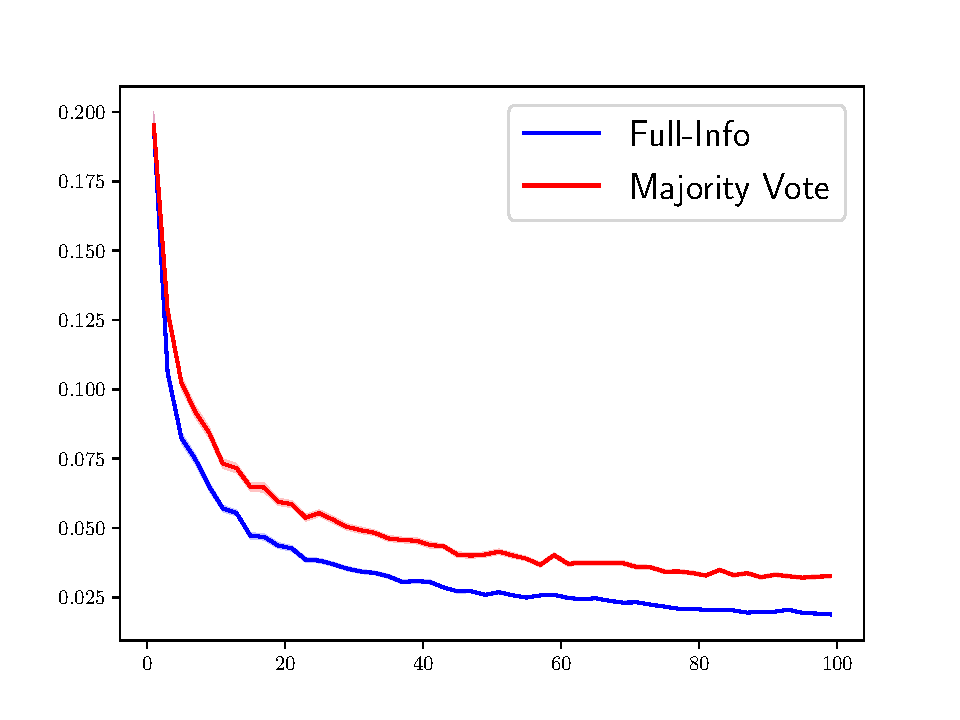
\includegraphics[width=0.3\textwidth]{figure/synthetic-class-05.pdf} &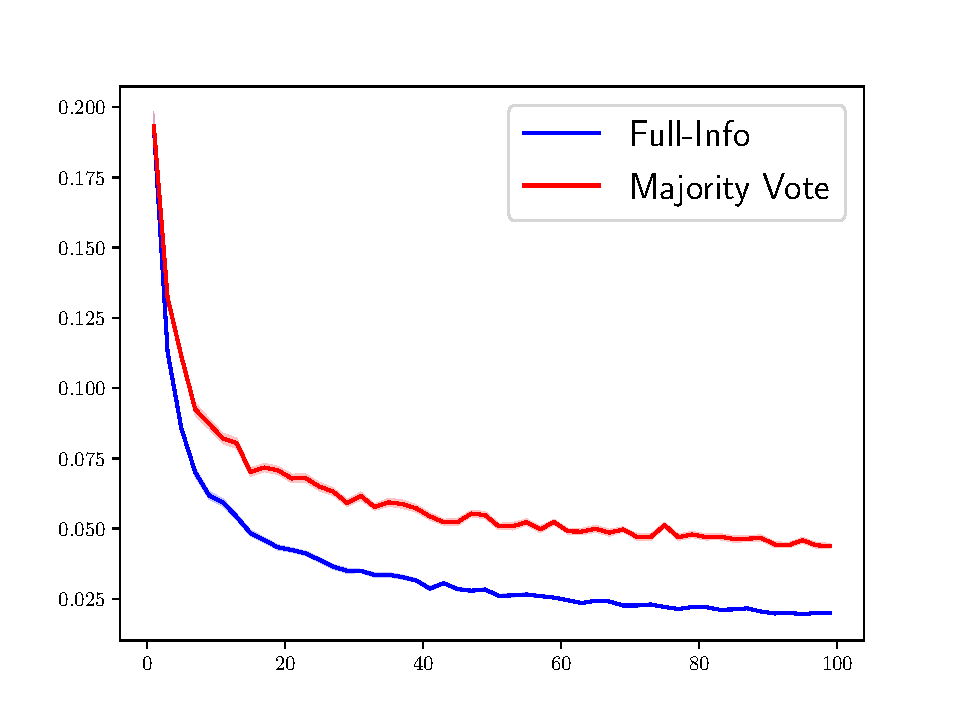
\includegraphics[width=0.3\textwidth]{figure/synthetic-class-10.pdf} &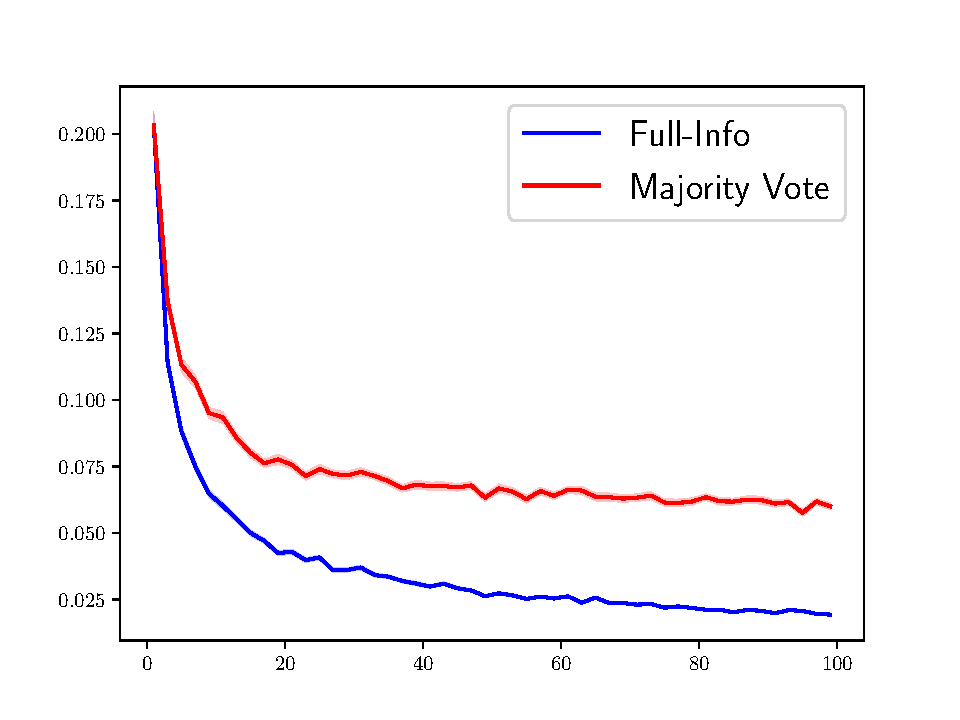
\includegraphics[width=0.3\textwidth]{figure/synthetic-class-15.pdf} \\
%% %		(a) & (b) & (c) \\
%% %		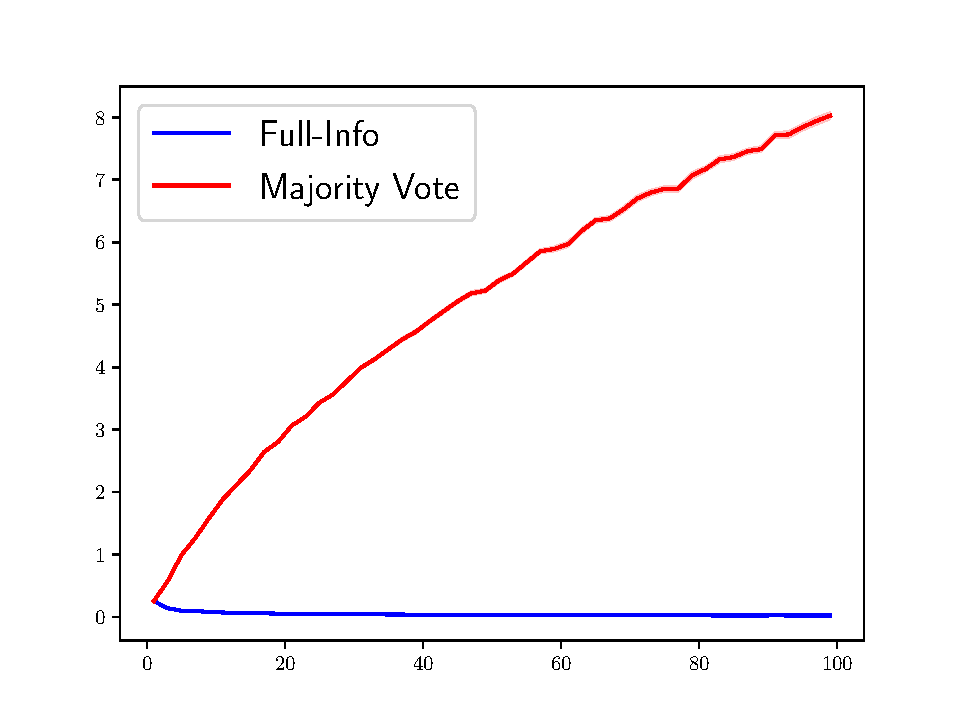
\includegraphics[width=0.3\textwidth]{figure/synthetic-calib-05.pdf} & 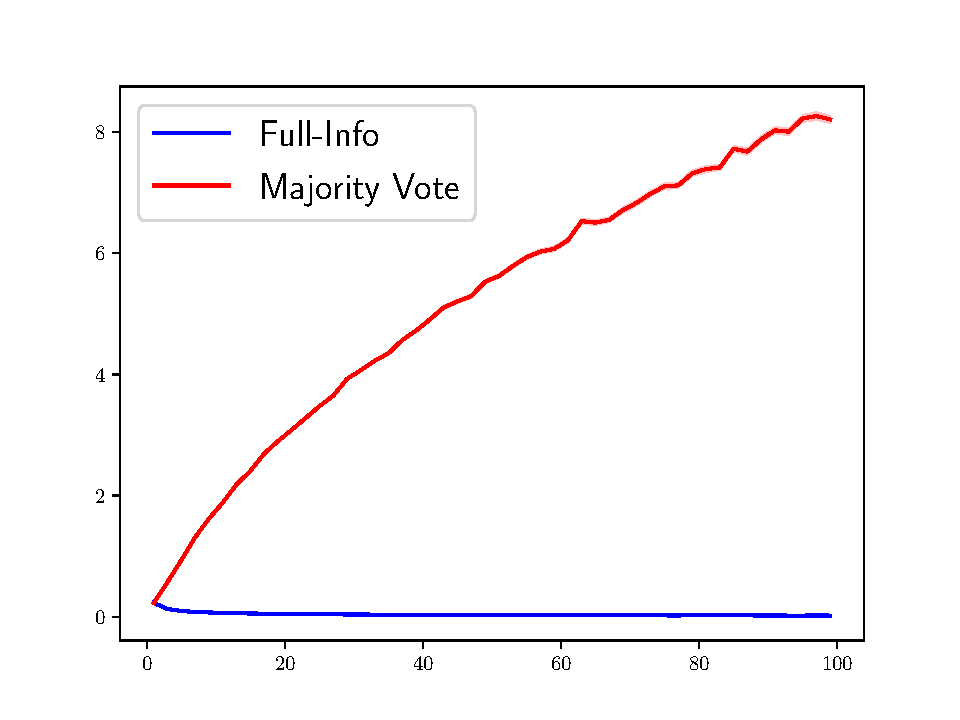
\includegraphics[width=0.3\textwidth]{figure/synthetic-calib-10.pdf} & 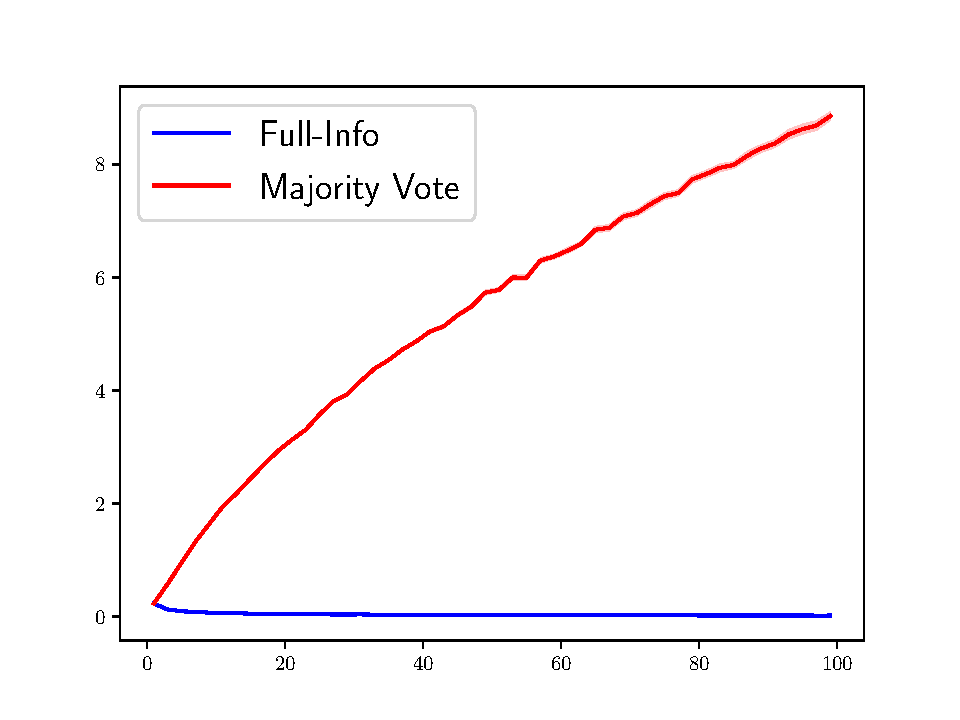
\includegraphics[width=0.3\textwidth]{figure/synthetic-calib-15.pdf}\\
%% %		(a) & (b) &  (c)
%% %	\end{tabular}
%% %	\caption{Classification error and calibration error for synthetic data for $n=1,000$ and $d=10$. For (a) $\beta = 0.5$; For (b) $\beta = 1$; For (c) $\beta = 1.5$. The errors are averaged over 100 trials with 95\% confidence bands.} \label{fig:synthetic}
%% %\end{figure}\ha{can we have only one legend in the plot?}



\subsection{BlueBirds}
\label{sec:BB}

We begin with the
\href{https://github.com/eaplatanios/noisy-labels}{BlueBirds}
dataset~\cite{WelinderBrPeBe10}, a small dataset of 108 images with ResNet features.  The task is to classify each image as one of
\textit{Indigo Bunting} or \textit{Blue Grosbeak} (two similar-looking blue
bird species). For each image, we have $39$ labels, obtained through Amazon
Mechanical Turk workers.  We use an ImageNet pretrained
ResNet50 model to generate image
features, applying PCA to reduce the dimensionality from
$d_{\textup{init}} = 2048$ to $d=25$.

We repeat the following experiment $T = 100$ times.
%
For each number $m = 1, \ldots, 35$ of labelers, we fit
the multi-label logistic model~\eqref{eq:maximum-likelihood}
and the majority vote estimator~\eqref{eq:logistic-majority},
finding calibration and classification errors using 10-fold cross validation.
%
We measure calibration error on an example $x$
by $|\logit(\wt{p}(x)) -
\logit(\what{p}(x))|$, where $\wt{p}(x)$ is the predicted probability,
$\what{p}(x)$ the empirical labeler probability,
and $\logit(p) = \log\frac{p}{1 - p}$; we measure classification
error on example $x$ with
labels $(y_1, \ldots, y_m)$ by $\frac{1}{m} \sum_{j = 1}^m \ind\{y_j \neq
\sgn(\wt{p}(x) - \half)\}$, giving an inherent noise floor because
of labeler uncertainty. We
report the results in Figure~\ref{fig:bluebird}.
These plots corroborate
our theoretical predictions: as the number of labelers $m$ increases, both
the majority vote method and the full label method exhibit improved
classification error, but considering all labels gives a (significant)
improvement in accuracy and in calibration error.

%we train the last layer of a pre-trained model \ha{which dataset for pretraining?} using the two algorithms of interest.
%
%
% \ha{why} and the images are noisy \ha{what does that mean?}.
%For each image
%The dataset was constructed by labels of 39 Amazon MTurk workers, with each of them labeling every image \textit{Indigo Bunting} or \textit{Blue Grosbeak}. For each image $i$, we generate their features $x_i \in \R^d$ by first taking the last layer outputs of a pretrained neural network $\tilde{x}_i \in \R^D$ and using PCA to reduce $\begin{bmatrix} \tilde{x}_1 & \cdots & \tilde{x}_n \end{bmatrix}^\top \in \R^{n \times D}$ to $\begin{bmatrix} x_1 & \cdots & x_n \end{bmatrix}^\top \in \R^{n \times d}$. The plots are shown in Fig.~\ref{fig:bluebird}.



\begin{figure}[ht]
  %% \vspace{-.6cm}
  \begin{center}
    \begin{tabular}{cc}
      \begin{overpic}[width=.48\columnwidth]{%,grid]{%
	  figure/resnet-class-bluebirds.pdf}
	\put(30,-1){{\small Number of labelers $m$}}
	\put(-3,20){
	  \rotatebox{90}{{\small Classification error}}}
      \end{overpic} &
      \hspace{-.3cm}
      \begin{overpic}[width=.48\columnwidth]{%,grid]{%
	  figure/resnet-calib-bluebirds.pdf}
	\put(30,-1){{\small Number of labelers $m$}}
	\put(-3,20){
	  \rotatebox{90}{{\small Calibration error}}}
      \end{overpic} \\
      (a) & (b)
    \end{tabular}
    \caption{\label{fig:bluebird} Experiments on BlueBirds dataset. (a)
      Classification error.  (b) Calibration error $|\logit(\wt{p}) -
      \logit(p)|$ with ResNet features reduced via PCA to dimension
      $d=25$. Error bars show 2 standard error confidence
      bands over $T = 100$ trials.}
  \end{center}
\end{figure}



\subsection{Crowdsourcing methods on semisynthetic CIFAR-10 labels}
\label{sec:semi-synthetic}


\newcommand{\softmax}{\textup{softmax}}

We adapt the original
CIFAR-10 dataset~\cite{KrizhevskyHi09}, which consists of 6000 $32 \times
32$ images from each of $k = 10$ classes (60,000 total images).
%
To mimic collecting messy data, rather than the single-label
in the base CIFAR-10 data, we construct pseudo-labelers
using a pretrained eighteen layer residual network
$f: \mc{X} \to \R^k$ (ResNet18~\cite{HeZhReSu16}) whose accuracy we can
adjust.
%
For $s \in \R^k$, define $\softmax(s) = [e^{s_y} /
  \sum_{l = 1}^k e^{s_l}]_{y = 1}^k$.
%
Then for an input $x \in \mc{X}$, the model outputs a score $f(x)
= {\Theta\opt}^\top \phi(x) \in \R^k$, where
$\Theta\opt = [\theta_1\opt ~ \cdots ~ \theta_k\opt] \in \R^{d \times k}$
is a matrix of per-class weights and
$\phi : \mc{X} \to \R^d$ represents the second-to-last layer
outputs of the neural network.
%
%% \in
%% \R^k$, where $\softmax(f(x))$ indicates the probabilities $\P(Y = y \mid X =
%% x)$.  The model $f$ has the form
%% \begin{equation*}
%%   f(x) = {\Theta\opt}^\top \phi(x), \qquad \text{s.t. }\Theta\opt = [\theta\opt_1 ~ \cdots ~ \theta\opt_k] \in \R^{d \times
%%   	k},
%% \end{equation*}
%% where $\Theta\opt$ is a matrix of per-class weights, and $\phi : \mc{X} \to \R^d$
%% represents the second-to-last layer outputs of the neural network. 
%
As we fit linear models, we take the outputs $\phi(x_i)$ as data, so
$X_i = \phi(x_i)$ are the covariates for the $i$th image $x_i$,
and $\Theta\opt$
is the ground-truth parameter.  We construct labels $Y_{ij}
\in \{1, \ldots, k\}$, $j = 1, \ldots, m$
by choosing the constant $\alpha > 0$
to model labeler expertise, drawing
\begin{equation*}
  \P(Y_{ij} = y \mid X_i = x)
  = \softmax(\alpha f(x))_y
  %% = \softmax(\alpha {\Theta\opt}^\top \phi(x))_y
  = \frac{\exp(\alpha \<\theta\opt_y, \phi(x)\>)}{
    \sum_{l = 1}^k \exp(\alpha \<\theta\opt_l, \phi(x)\>)}.
\end{equation*}
We vary $\alpha$ in experiments to adjust that the median value
of $p_i \defeq \max_{y \in [m]} \softmax(\alpha f(x_i))_y$, where
$p_i \in (1/k, 1)$. In the ``expert labelers'' case, we take
$\alpha \to \infty$ so that $\mbox{median}(\{p_i\}) \to 1$,
while the ``crowd labelers'' case corresponds to
$\alpha \downarrow 0$ and $\mbox{median}(\{p_i\}) \to 1/k$.

We fit $\mve$ and
$\what{\theta}^{\textup{mle}}_{n,m}$ using the multiclass logistic loss.
%
To test our predictions, we also investigate the standard
Dawid-Skene (DS)~\cite{DawidSk79} and GLAD~\cite{WhitehillWuBeMoRu09}
crowdsourcing methods.
%
The DS method models the probability that labeler $j$ assigns label $y'$
given correct label $y$ through a matrix $\alpha_j \in \R^{k \times k}$ with
$p_j(y' \mid y) = \frac{1}{1 + e^{-\alpha_j(y', y)}}$, while GLAD estimates
the probability that labeler $j$ correctly identifies the label of an
example $i$ via $p_{ij} = \frac{1}{1 + e^{-\beta_i \alpha_j}}$, where
$\alpha_j \in [-\infty,\infty]$ indicates labeler $j$'s ability and
$\beta_i \in [0, \infty]$ ambiguity in example $i$.
%
Each method uses EM to approximately maximize the likelihood $\prod_{i =
  1}^n \prod_{j = 1}^m \Prb(Y_{ij} \mid \alpha_j, \beta_i)$ (letting
$\beta_i = 1$ for DS) of the observed labels $Y_{ij}$,
initializing $\alpha$ to maximize the likelihood $\prod_{i = 1}^n \prod_{j
  = 1}^m \Prb(Y_{ij} \mid \majY_i, \alpha_j, \beta_i)$ assuming the majority
votes $\majY_i$ are correct and $\beta_i = 1$.
%
Given estimates $\what{\alpha}$ and $\what{\beta}$, one may impute soft
labels $\what{p}_i \in \R_k^+$ for each example $i$, where $\what{p}_{iy}$
indicates the method's estimated probability that example $i$ is of class
$y$, and hard labels $\what{Y}_i = \argmax_y \what{p}_{iy}$.
%
The labels yield  estimators from, respectively, hard and soft labels via
\begin{equation*}
  \what{\theta}_{\textup{h}}
  = \argmin_{\theta_1, \ldots, \theta_k}
  \sum_{i = 1}^n \log\bigg(\sum_{l = 1}^k
  e^{\<X_i, \theta_l - \theta_{\what{Y}_i}\>}\bigg)
  % \exp(\<X_i, \theta_l - \theta_{\what{Y}_i})\right)
  ~~ \mbox{and} ~~
  \what{\theta}_{\textup{s}}
  = \argmin_{\theta_1, \ldots, \theta_k}
  \sum_{i = 1}^n
  \sum_{y = 1}^k
  \what{p}_{iy} \log\bigg(\sum_{l = 1}^k
  e^{\<X_i, \theta_l - \theta_y\>} \bigg).
  % \exp(\<X_i, \theta_l - \theta_y\>\right),
\end{equation*}
We let $\dse$
and $\glade$ denote the corresponding estimators using hard labels,
and $\dspe$ and $\gladpe$ those trained with the estimated
probabilities $\what{p}_i$.
%
Our experiments use
Crowd-Kit~\citep{UstalovPaTs24}.

\begin{figure}[ht]
  %% \vspace{-.6cm}
  \begin{center}
    \begin{tabular}{cc}
      \hspace{-2cm}
      \begin{overpic}[width=.65\columnwidth]{%,grid]{%
	  figure/hard-test-error.pdf}
      \end{overpic} &
      \hspace{-2.5cm}
      \begin{overpic}[width=.65\columnwidth]{%,grid]{%
	 figure/soft-test-error.pdf}
      \end{overpic} \\
      \hspace{-2cm} (a) &
      \hspace{-2.5cm} (b) \\
      \hspace{-2cm}
      \begin{overpic}[width=.5\columnwidth]{%,grid]{%
	  figure/105.pdf}
      \end{overpic} &
      \hspace{-2.5cm}
      \begin{overpic}[width=.5\columnwidth]{%,grid]{%
	  figure/42.pdf}
      \end{overpic} \\
      \hspace{-2cm} (c) & \hspace{-2.5cm} (d)
    \end{tabular}
    \caption{\label{fig:semisynthetic} Experiments on semisynthetic
      CIFAR-10 dataset. Median labeler accuracy represents the
      median of $p_i = \max_y \softmax(\alpha f(x_i))_y$
      on the training data. Results are
      averaged over $20$ trials, and vertical axes
      give mis-classification rate from (synthetic) ground-truth labels
      on held-out test set. Legend keys correspond to
      maximum likelihood $\what{\theta}^{\textup{mle}}_{n,m}$ (MLE),
      majority vote $\mve$ (MV), hard-labeled Dawid-Skene (DS) and
      GLAD crowdsourced estimators $\dse$ and $\glade$,
      and soft-labaled Dawid-Skene (DS prob) and GLAD (GLAD prob)
      estimators $\dspe$ and $\gladpe$.
      (a) Comparison of methods using hard labels.
      (b) Comparison with crowdsourced estimated soft-labels.
      (c) Number of labelers $m$ versus test error for
      median accuracy $p = .105$ (noisy labelers). (d)
      Number of labelers $m$ versus test error for
      median accuracy $p = .4$. Both (c) and (d) report
      95\% error bars over the trials.}
  \end{center}
\end{figure}

We report the results in Fig.~\ref{fig:semisynthetic}. As we see,
when the model is well-specified,
the MLE $\what{\theta}^{\textup{mle}}_{n,m}$ %%with soft labels 
outperforms aggregation methods and black-box crowdsourcing models that
generate soft labels. Crowdsourced $\dse$ and
$\glade$ yield smaller test error than $\mve$, and using the soft labels,
$\dspe$ and $\gladpe$ further reduces the error, suggesting benefits
to using soft labels from crowdsourcing for training even if the
underlying model is unknown.

\section{Discussion and extensions}

\paragraph{Semi-parametric approaches.}
\label{sec:semi-param}
\label{sec:master-results-sem}

Our analysis separates likelihood-based approaches using all the labels, as
in~\eqref{eq:maximum-likelihood}, and majority vote estimators, which are
robust but have slower convergence, as in
Proposition~\ref{prop:lowd-misspcfd-majority-vote-m}.
%
While we mainly focus on efficiency bounds for 
procedures we view as closer to practice,
%---fitting a model based on available data---
in this section, we
present a few extensions to semiparametric approaches, more
as an amuse-bouche to motivate further efficiency investigations
rather than as a final word.
%% We thus develop a few convergence results into which we can substitute
%% semiparametric estimators.
%
In distinction from standard results in semiparametric theory
(e.g.~\cite[Ch.~25]{VanDerVaart98} or~\cite{BickelKlRiWe98}), the results
require little more than consistent estimation of the links $\sigma_j\opt$
to recover (rate optimal) $1/m$ scaling in the asymptotic covariance.

Let $\vec{\sigma} = (\sigma_1, \ldots, \sigma_m)$
be potentially distinct labeler link functions
(with $\sigma_j\opt$ denoting the true links).
Then for
$(x, y) \in \R^d \times \{\pm 1\}^m$ define the link-based loss
\begin{equation*}
  \loss_{\vec{\sigma}, \theta}(y \mid x)
  \defeq \frac{1}{m} \sum_{j = 1}^m \loss_{\sigma_j,\theta}(y_j \mid x).
\end{equation*}
%
To eliminate ambiguity in $\vec{\sigma}$,
we normalize $\ltwo{\theta\opt} = 1$,
and then define the population loss
\begin{equation*}
	L(\theta, \vec{\sigma})
	\defeq \frac{1}{m} \sum_{j = 1}^m
	\E[\loss_{\sigma_j, \theta}(Y_j \mid X)].
\end{equation*}
For the sequence $\{\vec{\sigma}_n\} \subset \fsymlinksp$
of (estimated) links and data $(X_i,
Y_i)$, $Y_i = (Y_{i1}, \ldots, Y_{im})$, we define the semi-parametric
estimator
\begin{align*}
	\spe \defeq \argmin_{\theta \in \R^d}
	\frac{1}{n} \sum_{i = 1}^n
	\loss_{\vec{\sigma}_n, \theta}(Y_i \mid X_i).
\end{align*}

Both consistency and
asymptotic normality hold under appropriate convergence of
the link functions (see Appendix~\ref{sec:semi-supp} for details).
Define the distance $d_{\flink}$ on $\R^d
\times \flink$ by
\begin{align}
  d_{\flink}\left((\theta_1, \vec{\sigma}_1), (\theta_2, \vec{\sigma}_2)
  \right)
  \defeq
  \ltwo{\theta_1 - \theta_2}
  + \LtwoPbold{\vec{\sigma}_1(-Y\<X, u\opt\>)
    - \vec{\sigma}_2(-Y\<X, u\opt\>)}.
  \label{eqn:link-distance}
\end{align}
%We make the following assumption.
%\begin{assumption}
%	\label{assumption:sp-general}
%	The links $\vec{\sigma}\opt \in \fsymlinksp$ are normalized so
%	that $\P(Y_j = y \mid X = x) = \sigma\opt_j(y \<x, u\opt\>)$, and
%	the sequence $\{\vec{\sigma}_n\} \subset \fsymlinksp$ is consistent:
%	\begin{equation*}
%		\LtwoPbold{\vec{\sigma}_n(-Y\<X, u\opt\>)
%			- \vec{\sigma}\opt(-Y\<X, u\opt\>)}
%		\cp 0.
%	\end{equation*}
%	Additionally, the mapping $(\theta, \vec{\sigma}) \mapsto
%	\nabla_\theta^2 \poploss(\theta,
%	\vec{\sigma})$ is continuous for $d_{\fsymlinksp}$ at $(u\opt,
%	\vec{\sigma}\opt)$.
%\end{assumption}
%The continuity of $\nabla_\theta^2 \poploss(\theta, \vec{\sigma})$ 
%%$\nabla_\theta^2 \poploss(\theta, \vec{\sigma})$ at
%%$(u\opt, \vec{\sigma}\opt)$ 
%allows us to develop local asymptotic normality.
%To see we may expect the assumption to hold, we give reasonably simple
%conditions sufficient for it in Lemma~\ref{lem:d-continuity-guarantees}, Appendix~\ref{sec:semi-supp}.
Then
the next master result for semi-parametric
approaches characterizes the asymptotic behavior of the
semi-parametric estimator $\spe$ using the variance function
\begin{align*}
  C_{m, \vec{\sigma}\opt} := \frac{1}{m} \cdot
  \frac{\frac{1}{m} \sum_{j = 1}^m \E[\sigma_j\opt(Z) (1 - \sigma_j\opt(Z))]}{
    (\frac{1}{m} \sum_{j = 1}^m
    \E[{\sigma_j\opt}'(Z)])^2}.
\end{align*} 
\begin{theorem}
  \label{theorem:semiparametric-master-informal}
  Let Assumption~\ref{assumption:x-decomposition} hold and assume $|Z| > 0$
  has nonzero and continuous density $p(z)$ on $(0, \infty)$.  Suppose the
  sequence $\{\vec{\sigma}_n\}$ is consistent, i.e.,
  \begin{equation*}
    \LtwoPbold{\vec{\sigma}_n(-Y\<X, u\opt\>)
      - \vec{\sigma}\opt(-Y\<X, u\opt\>)}
    \cp 0,
  \end{equation*}
  the mapping $(\theta, \vec{\sigma}) \mapsto
  \nabla_\theta^2 \poploss(\theta,
  \vec{\sigma})$ is continuous for $d_{\flink}$ at $(u\opt,
  \vec{\sigma}\opt)$, and $\Ep [\ltwo{X}^4] < \infty$.  Then $\sqrt{n}(\spe - u\opt)$ is
  asymptotically normal, and the estimator $\what{u}\sem_{n,m} =
  \spe / \ltwos{\spe}$ satisfies
  \begin{equation*}
    \sqrt{n} \prn{\what{u}\sem_{n,m} - u\opt}
    \cd \normal\prn{0, 	C_{m, \vec{\sigma}\opt}
      \prn{\proj_{u\opt}^\perp \Sigma \proj_{u\opt}^\perp}^\dagger}.
  \end{equation*}
\end{theorem}
\noindent
Notably, Theorem~\ref{theorem:semiparametric-master-informal} exhibits optimal
$1/m$ covariance scaling whenever $\E[{\sigma\opt_j}'(Z)] \gtrsim 1$.

We give two example applications of the general
theory in Appendix~\ref{sec:semi-supp}: the first analyzing a full pipeline
for a single index model setting, which robustly estimates direction $u\opt$,
the link $\sigma\opt$, and then re-estimates $\theta\opt$; the second
assuming a stylized black-box crowdsourcing mechanism that provides
estimates of labeler reliability, highlighting how even in some
crowdsourcing scenarios, there could be substantial advantages to using full
label information.

\paragraph{Future work.}

In spite of the technical detail we require to prove our results,
we view this work as almost preliminary and hope that it inspires further
work on the full pipeline of statistical machine learning,
from dataset creation to model release.
%
Many questions remain.

On the theoretical side, we focus on a stylized model of
label aggregation, with majority vote---with the exception of the
crowdsourcing model above--functioning as the
stand-in for more sophisticated aggregation strategies. It seems challenging
to show that \emph{no} aggregation strategy can work as well as multi-label
strategies; it would be interesting to delineate the benefits
and drawbacks of more sophisticated denoising.
% We
% focus throughout on low-dimensional asymptotics, using asymptotic normality
% to compare estimators. 
Additionally, the insights make low-dimensional asymptotic predictions;
investigating high-dimensional scaling might yield new perspectives
as, for, classification datasets often become
separable~\cite{CandesSu19pnas}.
%%, which is consistent with modern
%%applied machine learning~\cite{ZhangBeHaReVi21}.
%but makes the asymptotics we
% derive impossible. One option
% is to investigate the asymptotics of maximum-margin estimators,
% which coincide with the limits of ridge-regularized logistic
% regression~\cite{RossetZhHa04, SoudryHoNaGuSr18}.

On the methodological and applied side, given the extent to which the
test/challenge dataset methodology drives progress in machine
learning~\cite{Donoho17}, it seems that developing newer datasets to
incorporate labeler uncertainty could yield substantial benefits.  A
particular refrain is that modern deep learning methods are overconfident in
their predictions~\cite{GoodfellowShSz15}; perhaps by
calibrating them to \emph{labeler} uncertainty we could
improve their robustness and performance.
%
Large-scale
models now frequently use only distantly supervised
labels~\cite{RadfordKiHaRaGoAgSaAsMiClKrSu21}, making
the study of appropriate data cleaning and collection more timely.
We look forward to deeper
investigations of the foundations of the full
practice of statistical machine learning.


%\subsection*{Support}
%
%This research was partially supported by the Office of Naval Research under
%awards N00014-19-2288 and N00014-22-1-2669, the Stanford DAWN Consortium,
%and the National Science Foundation grants IIS-2006777 and HDR-1934578.

\spacingset{1.87}

\documentclass[12pt]{article}
\usepackage{amsmath}
\usepackage{bibentry}
\usepackage{graphicx}
\usepackage{booktabs}
\usepackage{multirow}
\usepackage{url} % not crucial - just used below for the URL 

%\usepackage[final]{changes}
\usepackage[draft]{changes} 
\newcommand{\stkout}[1]{\ifmmode\text{\sout{\ensuremath{#1}}}\else\sout{#1}\fi} 
\setdeletedmarkup{\stkout{#1}}

%\pdfminorversion=4
% NOTE: To produce blinded version, replace "0" with "1" below.
\newcommand{\blind}{1}

% DON'T change margins - should be 1 inch all around.
\addtolength{\oddsidemargin}{-.5in}%
\addtolength{\evensidemargin}{-1in}%
\addtolength{\textwidth}{1in}%
\addtolength{\textheight}{1.7in}%
\addtolength{\topmargin}{-1in}%

\makeatletter
\def\input@path{}
\makeatother

\usepackage{geometry}
\geometry{verbose,tmargin=1in,bmargin=1in,lmargin=1in,rmargin=1in}

\usepackage{amsmath, amssymb, amsfonts, bm, mathtools}
\usepackage{amsthm}
\usepackage{xcolor}
\definecolor{darkblue}{rgb}{0,0,.5}
\usepackage{graphicx}
\usepackage{subfigure}

\newcommand{\theHalgorithm}{\arabic{algorithm}}

\usepackage[numbers]{natbib}

\usepackage[colorlinks=true,allcolors=darkblue]{hyperref}       % hyperlinks
\usepackage{url}            % simple URL typesetting
\usepackage{booktabs}       % professional-quality tables
\usepackage{amsfonts}       % blackboard math symbols
\usepackage{nicefrac}       % compact symbols for 1/2, etc.
\usepackage{microtype}      % microtypography

\allowdisplaybreaks

\usepackage{float}
\usepackage{multirow}
\usepackage{footnote}
\usepackage{dsfont}
% \usepackage{mathabx}

\usepackage{algorithm}
\usepackage{algorithmic}
\usepackage{nicefrac}


\usepackage{hyperref}
\usepackage[capitalize]{cleveref}
\usepackage{crossreftools}


\usepackage{tikz}
\usepackage{overpic}


\definecolor{cc}{RGB}{125,0,0}
\definecolor{jd}{RGB}{0,125,0}
\definecolor{ha}{RGB}{0,0,200}

\newcommand{\cc}[1]{\textcolor{cc}{[CC: #1]}}
\newcommand{\jd}[1]{\textcolor{jd}{[JD: #1]}}
\newcommand{\ha}[1]{\textcolor{ha}{[HA: #1]}}

 % \usepackage[inline]{showlabels}


% \newcommand{\Pr}{\mathsf{Pr}}

\usepackage{dsfont}


\newcommand{\ind}{\mathds{1}}
\newcommand{\var}{\mathsf{Var}}
\newcommand{\cov}{\mathsf{Cov}}
\newcommand{\Ep}{\mathbb{E}}
\newcommand{\E}{\mathbb{E}}
\newcommand{\Prb}{\mathbb{P}}
\newcommand{\R}{\mathbb{R}} % real numbers
\newcommand{\N}{\mathbb{N}} % natural numbers
\newcommand{\Z}{\mathbb{Z}} % integers
\renewcommand{\P}{\mathbb{P}}
\newcommand{\mc}[1]{\mathcal{#1}}
\newcommand{\brc}[1]{\left\{{#1}\right\}}
\newcommand{\prn}[1]{\left({#1}\right)} % parentheses
\newcommand{\prnbig}[1]{\big({#1}\big)} % parentheses
\newcommand{\prns}[1]{({#1})} % parentheses small
\newcommand{\prnBig}[1]{\Big({#1}\Big)} % parentheses
\newcommand{\prnBigg}[1]{\Bigg({#1}\Bigg)} % parentheses
\newcommand{\brk}[1]{\left[{#1}\right]} % bracket
\newcommand{\brkbig}[1]{\big[{#1}\big]} % parentheses
\newcommand{\brkBig}[1]{\Big[{#1}\Big]} % parentheses
\newcommand{\brkBigg}[1]{\Bigg[{#1}\Bigg]} % parentheses
\newcommand{\norm}[1]{\left\|{#1}\right\|} % norm
\newcommand{\normbig}[1]{\big\|{#1}\big\|} % norm
\newcommand{\abs}[1]{\left|{#1}\right|} % norm
\newcommand{\what}[1]{\widehat{#1}}
\newcommand{\wt}[1]{\widetilde{#1}}
\newcommand{\wb}[1]{\overline{#1}}
\newcommand{\wbmj}[1]{{#1}^+}
\newcommand{\majY}{Y^+}
\newcommand{\majmark}[1]{{#1}^+}
\newcommand{\sgn}{\mathsf{sign}}
\newcommand{\pred}{\mathsf{d}}
\newcommand{\dist}{\mathsf{dist}}
\newcommand{\NN}{\mathsf{NN}}
\newcommand{\normal}{\mathsf{N}}
\newcommand{\bindist}{\mathsf{Binomial}}
\newcommand{\maj}{\mathsf{maj}}
\newcommand{\dstr}{\mathcal{P}}
\newcommand{\lr}{^{\textup{lr}}}
\newcommand{\sem}{^{\textup{sp}}}
\newcommand{\cs}{^{\textup{cs}}}
\newcommand{\mv}{^{\textup{mv}}}
\newcommand{\ds}{^{\textsc{ds}}}
\newcommand{\dsp}{^{\textsc{ds-p}}}
\newcommand{\glad}{^{\textsc{glad}}}
\newcommand{\gladp}{^{\textsc{glad-p}}}
\newcommand{\amv}{^{\textup{amv}}}
\newcommand{\mm}{^{\textup{mm}}}
\newcommand{\proj}{\mathsf{P}}
\newcommand{\proju}{\proj_{u\opt}}
\newcommand{\projperp}{\proj_{u\opt}^\perp}
\newcommand{\Flink}{\mathcal{F}_{\mathsf{link}}}
\newcommand{\lipconst}{\mathsf{L}}
\newcommand{\loss}{\ell}
\newcommand{\poploss}{L}
\newcommand{\popsignloss}{L^{\textup{sgn}}}
\newcommand{\flink}{\mathcal{F}_{\mathsf{link}}}
\newcommand{\fsymlink}{\mathcal{F}_{\mathsf{link}}^0}
\newcommand{\fsymlinkL}{\mathcal{F}_{\mathsf{link}}^{\mathsf{L}}}
\newcommand{\fsymlinksp}{\mathcal{F}_{\mathsf{link}}^{\mathsf{sp}}}
% Norms for convenience, along with sizes
\newcommand{\lone}[1]{\norm{#1}_1} % l1 norm
\newcommand{\ltwo}[1]{\norm{#1}_2} % l2 norm
\newcommand{\linf}[1]{\norm{#1}_\infty} % l-infinity norm
\newcommand{\lzero}[1]{\norm{#1}_0} % l0 norm
\newcommand{\dnorm}[1]{\norm{#1}_*} % Dual norm
\newcommand{\lfro}[1]{\left\|{#1}\right\|_{\rm Fr}} % Frobenius norm
\newcommand{\ltv}[2]{\mathsf{TV}\prn{#1, #2}}
\newcommand{\matrixnorm}[1]{\left|\!\left|\!\left|{#1}
	\right|\!\right|\!\right|} % Matrix norm with three bars
\newcommand{\normbigg}[1]{\bigg\|{#1}\bigg\|} % A norm with 1 argument and bigg
% brackets.
\newcommand{\dnormbigg}[1]{\bigg\|{#1}\bigg\|_*} % A norm with 1 argument and bigg
% brackets.
\newcommand{\lonebigg}[1]{\normbigg{#1}_1} % l1 norm
\newcommand{\ltwobigg}[1]{\normbigg{#1}_2} % l2 norm
\newcommand{\ltwobig}[1]{\normbig{#1}_2} % l2 norm
\newcommand{\ltwoBig}[1]{\normBig{#1}_2} % l2 norm
\newcommand{\linfbigg}[1]{\normbigg{#1}_\infty} % l-infinity norm
\newcommand{\norms}[1]{\|{#1}\|} % A norm with 1 argument and normal (small)
% brackets.
\newcommand{\matrixnorms}[1]{|\!|\!|{#1}|\!|\!|} % Small matrix norm
\newcommand{\matrixnormbigg}[1]{\bigg|\!\bigg|\!\bigg|{#1}\bigg|\!\bigg|\!\bigg|} % Small matrix norm
\newcommand{\lones}[1]{\norms{#1}_1} % l1 norm with small brackets
\newcommand{\ltwos}[1]{\norms{#1}_2} % l2 norm with small brackets
\newcommand{\linfs}[1]{\norms{#1}_\infty} % l-infinity norm with small brackets
\newcommand{\lzeros}[1]{\norms{#1}_0} % l0 norm with small brackets

\newcommand{\opnorm}[1]{\matrixnorm{#1}_{\rm op}} % Operator norm with three bars
\newcommand{\opnormbigg}[1]{\matrixnormbigg{#1}_{\rm op}} % Operator norm with three bars
\newcommand{\opnorms}[1]{\matrixnorms{#1}_{\rm op}} % Small operator norm with three bars
\newcommand{\<}{\langle} % Angle brackets
\renewcommand{\>}{\rangle}

\DeclareMathOperator*{\argmax}{argmax}
\DeclareMathOperator*{\argmin}{argmin}

\newcommand{\sX}{\mathcal{X}} % input space
\newcommand{\sY}{\mathcal{Y}} % output space


\newcommand{\simiid}{\stackrel{\textup{iid}}{\sim}}
\newcommand{\indic}[1]{1\!\left\{{#1}\right\}}

\newcommand{\cd}{\rightsquigarrow}
% \newcommand{\cd}{\stackrel{d}{\rightarrow}}
\newcommand{\cp}{\stackrel{p}{\rightarrow}}
\newcommand{\cas}{\stackrel{a.s.}{\rightarrow}}

\makeatletter
\long\def\@makecaption#1#2{
  \vskip 0.8ex
  \setbox\@tempboxa\hbox{\small {\bf #1:} #2}
  \parindent 1.5em  %% How can we use the global value of this???
  \dimen0=\hsize
  \advance\dimen0 by -3em
  \ifdim \wd\@tempboxa >\dimen0
  \hbox to \hsize{
    \parindent 0em
    \hfil 
    \parbox{\dimen0}{\def\baselinestretch{0.96}\small
      {\bf #1.} #2
      %%\unhbox\@tempboxa
    } 
    \hfil}
  \else \hbox to \hsize{\hfil \box\@tempboxa \hfil}
  \fi
}
\makeatother

\newcommand{\defeq}{\coloneqq}
\newcommand{\Ltwo}[1]{\norm{#1}_{L^2}}
\newcommand{\LtwoP}[1]{\norm{#1}_{L^2(\Prb)}}
\newcommand{\LtwoPbold}[1]{\norm{#1}_{L^2(\Prb)}}
\newcommand{\LtwoPn}[1]{\norm{#1}_{L^2(\Prb_n)}}
\newcommand{\LtwoPns}[1]{\norms{#1}_{L^2(\Prb_n)}}
\newcommand{\LtwoQ}[1]{\norm{#1}_{L^2(Q)}}
\newcommand{\LtwoQn}[1]{\norm{#1}_{L^2(Q_n)}}
\newcommand{\LtwoQns}[1]{\norms{#1}_{L^2(Q_n)}}
\newcommand{\lipnorm}[1]{\norm{#1}_{\textup{Lip}}}

\newcommand{\half}{\frac{1}{2}}
\newcommand{\event}{\mc{E}}

\newcommand{\conv}{\textup{Conv}}
\newcommand{\card}{\textup{card}}
\newcommand{\starhull}{\textup{Star}}
\newcommand{\hinge}[1]{\left({#1}\right)_+}
\newcommand{\hinges}[1]{({#1})_+}

\newcommand{\red}[1]{\textcolor{red}{#1}}
\newcommand{\blue}[1]{\textcolor{blue}{#1}}
\newcommand{\darkblue}[1]{\textcolor{darkblue}{#1}}

\definecolor{innerboxcolor}{rgb}{.9,.95,1}
\definecolor{outerlinecolor}{rgb}{.6,0,.2}

\newcommand{\jcdcomment}[1]{\fcolorbox{outerlinecolor}{innerboxcolor}{
    \begin{minipage}{.9\textwidth}
      \red{\bf JCD Comment:} {#1}
  \end{minipage}} \\
}

\newcommand{\opt}{^\star}
\newcommand{\subopt}{_\star}
\newcommand{\gme}{\what{\theta}_{n,m}} %General multilabel estimator
\newcommand{\tmle}{\what{\theta}\lr_{n,m}} %MLE estimator without aggregation (logistic regression)
\newcommand{\mve}{\what{\theta}\mv_{n,m}} %Majority vote estimator
\newcommand{\spe}{\what{\theta}\sem_{n,m}} %Semiparametric estimator
\newcommand{\csmle}{\what{\theta}\cs_{n,m}} %Crowdsourcing estimator
\newcommand{\dse}{\what{\theta}\ds_{n,m}} %Dawid-Skene estimator
\newcommand{\dspe}{\what{\theta}\dsp_{n,m}} %Dawid-Skene soft estimator
\newcommand{\glade}{\what{\theta}\glad_{n,m}} %GLAD estimator
\newcommand{\gladpe}{\what{\theta}\gladp_{n,m}} %GLAD soft estimator
\newcommand{\G}{\mathbb{G}}


% \usepackage{enumerate}
\usepackage{enumitem}

\newtheorem{claim}{Claim}[section]
\newtheorem{lemma}[claim]{Lemma}
\newtheorem{assumption}{Assumption}
\newtheorem{definition}{Definition}
\newtheorem{theorem}{Theorem}
\newtheorem{example}{Example}
\newtheorem{proposition}{Proposition}
\newtheorem{remark}{Remark}
\newtheorem{corollary}{Corollary}
\renewcommand{\theassumption}{A\arabic{assumption}}
\renewcommand{\bindist}{\mathsf{Bin}}

\usepackage{xr}
\externaldocument{JASA-supp}

\begin{document}

%\bibliographystyle{natbib}

\def\spacingset#1{\renewcommand{\baselinestretch}%
{#1}\small\normalsize} \spacingset{1}

%%%%%%%%%%%%%%%%%%%%%%%%%%%%%%%%%%%%%%%%%%%%%%%%%%%%%%%%%%%%%%%%%%%%%%%%%%%%%%

\if1\blind
{
  \title{\bf How many labelers do you have? \\
  	A closer look at gold-standard labels}
  \author{Chen Cheng\thanks{Department of Statistics, Stanford University; email: \texttt{chencheng@stanford.edu}.} \and
  	Hilal Asi\thanks{Department of Electrical Engineering, Stanford University; email: \texttt{asi@stanford.edu}.}
  	\and
  	John Duchi\thanks{Departments of Statistics and Electrical Engineering, Stanford University; email: \texttt{jduchi@stanford.edu}.}}
  \maketitle
} \fi

\if0\blind
{
  \bigskip
  \bigskip
  \bigskip
  \begin{center}
    {\LARGE\bf How many labelers do you have? \\
    	A closer look at gold-standard labels}
\end{center}
  \medskip
} \fi

\bigskip

% -*- mode: latex -*- %

\begin{abstract}
  The construction of most supervised learning datasets revolves around
  collecting multiple labels for each instance, then aggregating the labels
  to form a type of ``true'' label.
  %
  We question the wisdom of this pipeline by developing a (stylized)
  theoretical model of this process and analyzing its statistical
  consequences, showing how access to non-aggregated label information can
  make training well-calibrated models more feasible than it is with
  cleaned labels.
  %
  The entire story, however, is subtle, and the
  contrasts between aggregated and fuller label information depend on
  the particulars of the problem,
  where estimators that use aggregated information exhibit robust but slower
  rates of convergence, while estimators that can effectively
  leverage all labels converge more quickly \emph{if} they have
  fidelity to (or can learn) the true labeling process.
  The theory
  makes several predictions for real-world datasets, including when
  non-aggregate labels should improve learning performance, which we
  test to corroborate the validity of our predictions.
\end{abstract}


\noindent%
{\it Keywords:} Label aggregation, classification and calibration, crowdsourcing
\vfill

\newpage
\spacingset{1.87} % DON'T change the spacing!

% -*- Mode: latex -*- %

\section{Introduction}

Challenge datasets drive advances in statistical machine
learning~\cite{MarcusSaMa94, LewisYaRoLi04, AsuncionNe07, KrizhevskyHi09,
  DengDoSoLiLiFe09, RussakovskyDeSuKrSaMaHuKaKhBeBeFe15},
making the collection of
labeled data essential~\cite{Donoho17}.
%
While in the past, experts could label reasonably sized datasets, the cost
and size of modern datasets often precludes such annotation, motivating
crowdsourcing and other dataset generation strategies that aggregate
non-expert and expert feedback~\citep{DawidSk79,
  WhitehillWuBeMoRu09, RussakovskyDeSuKrSaMaHuKaKhBeBeFe15,
  CodellaRoTsCeDuGuHeKaLiMa19, GadreEtAl23}.
%% SchuhmannBeVeGoWiChCoKaMuWoScKuCrScKaJi22,
%
Frequently, published data contain aggregated label information; for
example, in the dataset~\cite{CodellaRoTsCeDuGuHeKaLiMa19}
%% RotembergKuBeCaChCoCoDuGuGu21}
of skin lesion images to be classified as
malignant, biopsy and histology confirm positive examples, while physician
consensus determines negative examples, yet the published data includes no
notion of disagreement or uncertainty in these consensuses.
%
Similarly, the benchmark CIFAR~\citep{KrizhevskyHi09} and
ImageNet~\citep{DengDoSoLiLiFe09, RussakovskyDeSuKrSaMaHuKaKhBeBeFe15}
computer vision challenges include only a single label for each example, in
spite of deriving from multiple pieces of feedback per image.
%
Researchers typically perform such aggregation in effort to obtain
``high-quality'' or ``true'' labels~\cite{DengDoSoLiLiFe09,
  RussakovskyDeSuKrSaMaHuKaKhBeBeFe15, DawidSk79,
  WhitehillWuBeMoRu09}.

Yet most statistical machine learning development does not investigate this
full data generating process, assuming only that data comes in the form of
$(X, Y)$ pairs of covariates $X$ and labels $Y$~\cite{Vapnik95,
  BoucheronBoLu05, BartlettJoMc06, HastieTiFr09}.
%
We argue for a more
holistic perspective: that analysis and algorithmic development should focus
on the complete statistical learning pipeline, from dataset construction to
model output.
%
We question the extent to which such label cleaning strategies are
essential, arguing that benchmark datasets ought to include noisy labels as
a rule; one may always clean the data in subsequent stages, but sometimes
the more nauced labeling information may yield more accurate downstream
models.

%\cc{Also the second perspective---the crowdsourcing community aims to obtaining labels as clean as possible but largely ignoring how it would affect downstream tasks, or simply assuming the goal is to clean the labels as much as possible. Our results suggest (i) maybe the correct upstream tasks is not to get gold-standard labels; (ii) provided we can get multilabeled data from upstream tasks, we essentially have a different statistical learning model from the classical ones which makes it possible for us to do more.} 

%% We revisit this data generation process and question its aggregation
%% strategies.  While it is tempting to apply majority-vote aggregation to
%% obtain an expert label, resembling a typical machine learning dataset, this
%% ignores the inherent uncertainty and noise in this pipeline.  There has been
%% numerous amounts of work from the crowd-sourcing
%% community~\cite{WhitehillWuBeMoRu09,WelinderBrPeBe10,TianZh15} (see
%% Section~\ref{sec:related-work} for more details) that \emph{experimentally}
%% study the above process and design better algorithms by taking into
%% consideration the inherent noise in the labels. However, a complete
%% (theoretical) understanding of this process and the effects of uncertainties
%% and other important problem parameters---such as number of labelers and data
%% noise---is still lacking.

We develop a stylized theoretical model to capture uncertainty in the
labeling process, allowing us to understand the limitations of and possible
improvements to using aggregated data in a statistical learning pipeline.
%
We model each example as a pair $(X_i, (Y_{i1},\dots,Y_{im}))$ where $X_i$
is a data point and $Y_{ij}$ are noisy binary labels.
%
The basic
formulation of our results compares two methods: empirical risk
minimization using all labels and empirical risk minimization using
majority vote labels $\majY$.
%
While this oversimplifies label
aggregation strategies~\cite{DawidSk79, RussakovskyDeSuKrSaMaHuKaKhBeBeFe15,
  RatnerBaEhFrWuRe17},
the simplicity (i) allows us to understand
fundamental limitations of algorithms based on majority-vote aggregation,
(ii) facilitates circumventing these limits via non-aggregated
information, and (iii) provides a base for future work: the purposeful
simplicity permits classical tools to apply.
%
In these models, our results show that estimators using non-aggregated labels
outperform those that use aggregated (majority-vote)
labels if the predictive model has fidelity to the data,
majority-vote estimators provide robust (but slower) convergence, and these
tradeoffs are fundamental.
%
We extend the results to include misspecification, semiparametric
scenarios, and simple models of learned annotator reliability.

While our models are stylized, they make testable predictions for real data
beyond simplified scenarios, in particular, that models fit on
non-aggregated data should both make better-calibrated predictions and have
lower classification error than those using cleaned labels.
%
Experiments on two real and one large semisynthetic dataset corroborate the
implications of our theory beyond logistic models: majority-vote-based
algorithms yield uncalibrated predictors, while algorithms using full label
information provide (more) calibrated predictors.
%
The former algorithms exhibit worse classification error in our experiments,
with the error gap depending on parameters---e.g.,
noise---we address in our theoretical models.
 

\subsection{Problem formulation}
\label{sec:formulation}

%% To situate our results, we begin by
%% providing the key ingredients in the paper.

% \paragraph{The label model.}
Consider covariates $X_i \simiid \P_X$, $X_i \in \R^d$, in a
binary classification problem with $m$ labelers,
who annotate points independently through a generalized linear
model (GLM) via link functions %% $ \flink$, where
\begin{align*}
  \sigma_1\opt, \dots,
  \sigma_m\opt \in \flink := \brc{\sigma : \R \to [0, 1]
    \mid \sigma(0) = 1/2, \sgn(\sigma(t) - 1/2) = \sgn(t)}.
\end{align*} 
%% Here $\sgn(t) = -1$ for $t <0$, $\sgn(t) = 1$ for $t > 0$ and $\sgn(0) = 0$. 
For example, in the logistic model where
labelers have identical link, $\sigma_j\opt(t) = 1 / \prn{1 + e^{-t}}$.
%
If $\sigma(t) + \sigma(-t) = 1$ for all $t \in \mathbb{R}$, we say the
link function is symmetric, denoting the class of symmetric
links by $\fsymlink \subset \flink$.
%
Labels then follow the distribution
\begin{align}
  \Prb_{\sigma, \theta}(Y = y \mid X = x) & =
  \sigma ( y \< \theta, x\>) ~~~ \mbox{for~} y \in \left\{\pm 1\right\},
  ~ x,\theta \in \R^d. \label{eq:general-calibration-model}
\end{align}
Key to our model, and what allows our analysis, is that we assume
labelers use the same linear classifier $\theta\opt \in \R^d$, %%---though each
%%labeler $j$ may have a distinct link $\sigma_j\opt$---
so we obtain conditionally independent labels $Y_{ij} \sim \Prb_{\sigma_j\opt,
  \theta\opt}(\cdot \mid X_i)$.
 We
seek to recover $\theta\opt$ or the direction $u\opt := \theta\opt /
\ltwo{\theta\opt}$ from the observations $(X_i, Y_{ij})$.

\paragraph{Error measures.}
We evaluate an estimator $\what{\theta}$ and associated direction $\what{u}
\defeq \what{\theta} / \ltwos{\what{\theta}}$ through
\begin{enumerate}[leftmargin=10em,label=(\textsc{E}.\roman*)]
\item \label{item:class}
  The classification error: $\ltwos{u\opt - \what{u}}
  = \sqrt{2(1 - \<u\opt, \what{u}\>)}$.
  % \tag{\textsc{E.class}
\item \label{item:cal}
  The calibration error:~~ $\ltwos{\theta\opt - \what{\theta}}$.
\end{enumerate}
%% \begin{align*}
%%   \textbf{(i)} & \quad \text{The classification error:} ~~ ~\|u^\star - \what{u}\|_2 = \sqrt{2(1 - \langle u\opt, \what{u} \rangle)}. \\
%%   \textbf{(ii)} & \quad
%%   \text{} ~~~~ ~~ \|\theta^\star - \what{\theta}\|_2.
%% \end{align*}
To motivate these errors, note that for classification, we only need to
control the difference between the directions $\what{u}$ and $u\opt$, while
calibration---that for a data point $X$, the value $\sigma_j\opt( \<
\what{\theta}, X \>)\approx \sigma_j\opt(\< \theta\opt, X \>)$---requires
controlling the error in $\what{\theta}$ as an estimate of $\theta\opt$.
%
If $X$ is rotationally symmetric,
then $\P(\sgn(\<X, u\>) \neq \sgn(\<X, u\opt\>)) = \frac{1}{\pi}
\cos^{-1}\<u, u\opt\>$ for any unit vectors $u, u\opt$; because $\cos^{-1} t
= (1 + o(1)) \sqrt{2(1 - t)}$ as $t \uparrow 1$, the classification
error~\ref{item:class}, $\ltwo{u\opt - u} =
\sqrt{2(1 - \<u, u\opt\>)}$, is asymptotically equivalent to the angle
between $u$ and $u\opt$.

\paragraph{Estimators.}
We consider two types of estimators: one
using processed labels $\majY_i$ for each
example $X_i$, and the other
using each label $Y_{i1}, \ldots, Y_{im}$.
%
To center discussion, we instantiate this temporarily via logistic
regression for the logistic link $\sigma\lr(t) = \frac{1}{1 + e^{-t}}$,
defining
\begin{align*}
  \loss_\theta\lr(y \mid x) = -\log \Prb_{\sigma\lr, \theta}(y \mid x)
  = \log(1 + e^{-y\<x,\theta\>})  .
\end{align*}
In the non-aggregated model, we let let $\Prb_{n,m}$ be the empirical
measure on $\{(X_i, (Y_{i1},\dots,Y_{im}))\}$ and consider the logistic
regression estimator (i.e., the MLE assuming the logistic model)
\begin{align}
  \label{eq:maximum-likelihood}
  \tmle = \argmin_\theta \left\{\Prb_{n,m} \loss_\theta\lr
  = \frac{1}{nm} \sum_{i = 1}^n \sum_{j = 1}^m \loss_\theta\lr(Y_{ij} \mid X_i)
  \right\}.
\end{align}
We focus on the simplest
aggregation strategy, where example $i$ has majority vote label
\begin{align*}
  \majY_i = \maj(Y_{i1}, \ldots, Y_{im})
  \defeq \sgn\left(\sum_{j=1}^m Y_{ij}\right)
  ~~~\mbox{where}~~~
  \sgn(0) \sim \mathsf{Ber}(1/2)
\end{align*}
%% (breaking ties randomly).
Then letting $\majmark{\Prb}_{n,m}$ be the empirical measure on
$\{(X_i, \majY_i)\}$, the majority-vote estimator solves
\begin{align}
  \label{eq:logistic-majority}
  \mve = \argmin_\theta  \brc{\majmark{\Prb}_{n,m}\loss_\theta\lr = \frac 1 n \sum_{i=1}^n  \loss_\theta\lr(\majY_i \mid X_i)}.
\end{align}
Method~\eqref{eq:logistic-majority} acts as our proxy for the ``standard''
data analysis pipeline, with cleaned labels, while
method~\eqref{eq:maximum-likelihood} is our proxy for non-aggregated methods
using all labels.
%
More general formulations than the majority
vote~\eqref{eq:logistic-majority} could allow complex aggregation
strategies, e.g., crowdsourcing, but we simplify to capture what we view as
the essentiae for problems (e.g.\ CIFAR~\cite{KrizhevskyHi09} or
ImageNet~\cite{RussakovskyDeSuKrSaMaHuKaKhBeBeFe15}) where only aggregated
label information is available.

Our main results characterize the
asymptotics of the
estimators $\mve$ and $\tmle$.
%
Under
appropriate assumptions on the data generating
mechanisms~\eqref{eq:general-calibration-model}, which include
misspecification, we (i) provide consistency results that elucidate the
limits for $\mve$, $\tmle$, and a few more general
estimators, and (ii) evaluate their limit distributions via
asymptotic normality. The latter allows comparison
of the estimators through their limiting covariances, which
exhibit (to us) interestingly varying dependence on $m$ and the scaling of
the true parameter $\theta\opt$.

\subsection{Summary of results and implications}

Asymptotic characterization of the
estimators~\eqref{eq:maximum-likelihood}--\eqref{eq:logistic-majority}
provides our main avenue to highlighting the import of multiple labels.
%
Table~\ref{table:comparisons}  summarizes our results, comparing
the performance of the MLE-type~\eqref{eq:maximum-likelihood} and
majority vote~\eqref{eq:logistic-majority} estimators for the
classification~\ref{item:class} and calibration~\ref{item:cal} errors.
%
We highlight estimator performance in two scenarios:
``single link'' corresponds to the case that the loss is
well-specified, while ``mis-specified''
corresponds to the case that $\loss_\theta(y \mid x) \neq -\log
\Prb_{\sigma,\theta}(y \mid x)$, which may occur when labelers have
distinct link functions $\sigma$ or the model is incorrect.
%
In all cases, the
estimate $\what{\theta}$ and
vector $\what{u} = \what{\theta} / \ltwos{\what{\theta}}$
are asymptotically normal around a scalar multiple of $\theta\opt$,
with differeing scaling and asymptotic variance.
%
With $m$ labelers,
each estimator yields a rate $r(m)$ and scale $t(m)$ for which
\begin{align}
  \label{eqn:limit-scaling-for-table}
  \sqrt{n}(\what{u} - u\opt)
  \cd \normal(0, r(m) \Sigma_{\textup{n}})
  ~~~ \mbox{and} ~~~
  \sqrt{n}(\what{\theta} - t(m) \theta\opt)
  \cd \normal(0, \Sigma_{\textup{u}}),
\end{align}
where $\Sigma_{\textup{n}}$ and $\Sigma_{\textup{u}}$ are ``normalized'' and
``unnormalized'' covariances, respectively.
%
The classification error~\ref{item:class} is small whenever $r(m) \ll 1$,
while the calibration error~\ref{item:cal} is small when $t(m) \approx 1$,
and Table~\ref{table:comparisons} shows the
scalings~\eqref{eqn:limit-scaling-for-table} for the different estimators.

\begin{table}
  \centering
  \begin{tabular}{c|c|c}
    \toprule 
    & MLE-type estimator~\eqref{eq:maximum-likelihood}
    & majority-vote estimator~\eqref{eq:logistic-majority} \\
    \hline
    single link
    & \textbf{Classification}:
    $r(m) \asymp \frac{1}{m}$
    & Classification: $r(m) \asymp \frac{1}{\sqrt{m}}$ \\
    (well-specified) & \textbf{Calibration}:
    $t(m) = 1$ &
    Calibration: $t(m) \asymp \sqrt{m}$ \\ 
    \hline
    mis-specified or
    & Calibration: $t(m) \asymp 1$ &  Calibration: $t(m) \asymp \sqrt{m}$  \\ 
    multiple links & Classification: $r(m) \asymp 1$ &
    \textbf{Classification}: $r(m) \asymp 1 / \sqrt{m}$
    \\
    \hline
  \end{tabular}
  \caption{
    Comparison of multi-label and majority-vote estimators
    for $X \sim \normal(0, I_d)$
    according to the scalings in classification error
    $r(m)$ and calibration error $t(m)$ that
    the limits~\eqref{eqn:limit-scaling-for-table} identify.
    %
    If $t(m) \gg 1$, the model is uncalibrated; if the rate $r(m)$ is small,
    the model achieves lower asymptotic variance.
    %
    Boldface indicates the associated estimator
    is (rate) optimal. \label{table:comparisons}}
\end{table}

%% We obtain several results clarifying the distinctions between
%% estimators that use aggregate labels from those that treat them
%% individually.

\paragraph{Improved performance using multiple labels for well-specified models}
%% As in our discussion above,
We begin in Section~\ref{sec:well-sepcified-mod} by specializing our main
results to the logistic model.
%
We show that the MLE~\eqref{eq:maximum-likelihood} is
calibrated and enjoys faster rates of convergence (in $m$) than the
majority-vote estimator~\eqref{eq:logistic-majority}.
%
The improvements depend on the underlying distribution, and
Propositions~\ref{prop:lowd-maximum-likelihood}
and~\ref{prop:lowd-majority-vote-m-noise} connect them to
Mammen-Tsybakov-type noise conditions.
%
In ``standard'' cases, the improvement scales as
$\sqrt{m}$; for problems with little classification noise, the majority vote
estimator becomes brittle (relatively slower), while the convergence rate
gap decreases for noisier problems.


\paragraph{Robustness of majority-vote estimators}
Our results also evidence support for majority vote
estimators~\eqref{eq:logistic-majority}.  Section~\ref{sec:mis-spec}
provides master results holding for well- and mis-specified losses, which
highlight the robustness of the majority vote estimator
(cf.\ Table~\ref{table:comparisons}).
%
The faster rates MLE-type estimators~\eqref{eq:maximum-likelihood} enjoy
when the model is correct break down in ways we make precise for
mis-specified models; in contrast, majority-vote-type
estimators~\eqref{eq:logistic-majority} maintain their (not quite optimal)
improved convergence guarantees, even under mis-specification, suggesting
practical value to cleaning data when correctly modeling uncertainty is
impossible.

\paragraph{Fundamental limits of majority vote}
Via local asymptotic minimax theory, Section~\ref{sec:lower-bound} develops
fundamental limits for estimation given only majority vote labels $(X,
\majY)$, which coincide with our results in
Section~\ref{sec:well-sepcified-mod}.
%
These results highlight how cleaned labels force slower
convergence in the number of labelers $m$ while reinforcing the claims of
robustness.
%
In particular, while a mis-specified link function introduces structural
bias that MLE-type estimators using all labels cannot overcome, majority
vote-based estimators achieve rate-optimal convergence for procedures
receiving cleaned labels $\majY$ (making the rate $r(m)$ in the bottom right
of Table~\ref{table:comparisons} sharp).

%% In particular, in both unspecified and well-specified cases, we cannot
%% achieve calibration---contrasting with non-aggregated data, which allows
%% calibrated estimators.

%with the simple result that any
%estimator based on majority vote aggregation cannot be calibrated:
%there exist distributions with distinct numbers of labelers $m$
%and link functions $\sigma$ that induce identical joint distributions on
%$(X, \majY)$.  This contrasts with non-aggregated data, which allows
%calibrated estimators.

%% (\Cref{sec:mis-spec}) we study the mis-specified model where the estimators
%% use a logistic model for the labelers which follow a different
%% model. Somewhat surprisingly, our results demonstrate that the majority vote
%% estimator is more robust to model mis-specification. In particular, it can
%% provide faster convergence rates than the multi-label estimator by a factor
%% of $\sqrt{m}$.

\paragraph{Experimental evaluation}
Our theoretical results predict two outcomes: (i) \emph{if} the
model has fidelity to the labeling process, then using all noisy labels
should yield better estimates than procedures using cleaned labels, and
(ii), that majority vote estimators should be more robust. In
Section~\ref{sec:experiments}, we thus provide real and semi-synthetic
experiments that corroborate the theoretical predictions; the experiments
also highlight a need, which some researchers are now beginning to
address~\cite{GadreEtAl23}, for more applied dataset development so that we
can evaluate the consequences of filtering and otherwise manipulating the
data we use.

\paragraph{Semi-parametric approaches}
%% The final theoretical component of the paper (Section~\ref{sec:semi-param})
%% provides an exemplar approach that puts the pieces together to achieve
%% efficiency via semi-parametric approaches. 
In our discussion (Section~\ref{sec:semi-param}), we include an exemplar
approach for estimation via semi-parametric approaches, where
one estimates labelers' links and reliability.
%
While not our main focus, the results provide potential insights into
estimation using existing crowdsourcing techniques, where black box
algorithms provide measures of labeler reliability that one may incorporate
to achieve rate-optimal estimation.


\subsection{Related work}
\label{sec:related-work}

%% We briefly overview related work, acknowledging that 
To make our theoretical model tractable, we capture only a few of the complexities inherent in
dataset construction. Label aggregation strategies often attempt to
evaluate labeler uncertainty, dating to~\citet{DawidSk79}, who study
labeler uncertainty estimation to overcome noise in
clinical patient measurements. With the rise of
crowdsourcing, such reliability models have
attracted interest, with approaches for optimal budget
allocation~\cite{KargerOhSh14}, addressing untrustworthy or malicious
labelers~\cite{CharikarStVa17}, and more broadly a line of applied~\cite{DengDoSoLiLiFe09, RussakovskyDeSuKrSaMaHuKaKhBeBeFe15} and theoretical work
studying crowd labeling and aggregation~\cite{WhitehillWuBeMoRu09,
  WelinderBrPeBe10, RatnerBaEhFrWuRe17}.
%%, with substantial
%% applications~\cite{DengDoSoLiLiFe09, RussakovskyDeSuKrSaMaHuKaKhBeBeFe15}.

Many of these focus, however, on obtaining a single
trustworthy label for each example. Our work takes a
different perspective.  First, we target statistical analysis for
the full learning pipeline---understanding the landscape of the
learning problem with multiple labels for each example---as opposed to
obtaining only clean labels. Moreover, we argue for
calibrating the resulting predictive model, which cleaned
labels necessarily impede. We therefore adopt a perspective similar to
the applied works~\citep{PetersonBaGrRu19,PlataniosAlXiMi20},
which highlight how incorporating human
uncertainty into learning pipelines can make classification ``more
robust''~\citep{PetersonBaGrRu19}.  Instead of splitting the learning
procedure into two phases, where the first aggregates labels and the second
trains, we use non-aggregated labels throughout
learning. \citet{PlataniosAlXiMi20} directly
model labeler reliability via a richer model than our stylized
scenarios, but our
approach allows theoretically precise description of the
methods' limiting
behavior.


Our results complement a growing body of work in machine learning.
%
The Neural Information Processing Systems conference
includes a Datasets and Benchmarks track, as they
``are crucial for the development of machine learning
methods''~\cite{BeygelzimerLiVaDa21},
%
%% As a particular examplar, \citet{GadreEtAl23} introduce DataComp,
%% a testbed for experimental work on datasets,
building off the long history
of dataset-driven development in machine learning~\cite{HardtRe22}.
%
We attempt to lay statistical foundations for this line of work.

%We mention in passing that our consistency results rely on
%distributional assumptions on the covariates $X$, for example,
%Gaussianity. That such technical conditions appear may be familiar from work,
%for example, in single-index or nonlinear measurement models~\cite{PlanVe16,
%  PlanVe13}. In such settings, one assumes $\E[Y \mid X] = f(\<\theta\opt,
%X\>)$ for an unknown increasing $f$, and it is essential that $\E[Y X]
%\propto \theta\opt$ to allow estimation of $\theta\opt$; we leverage similar
%techniques.

\paragraph{Notation}
For a matrix $M$, $\norm{M}$ denotes its spectral norm and $M^\dagger$ its
Moore-Penrose pseudo inverse.
%
For a unit vector $u$, $\proj_{u}^\perp \defeq
I - u u^\top$ projects to the space orthogonal to $\mathrm{span}\{u\}$.
%
We use the empirical process notation $\Prb Z = \int z d\Prb(z)$ and $\cd$
denotes convergence in distribution.
%
We write $f(x) \asymp g(x)$ for $x \in \R_+$ if there exist
numerical constants $0 < c_1, c_2 < \infty$ and $x_0 \geq 0$ such that $c_1
|g(x)| \leq |f(x)| \leq c_2|g(x)|$ for $x \geq x_0$,
and
$c = o_m(1)$ means $c \to 0$ as $m \to \infty$.


\section{The well-specified logistic model}\label{sec:well-sepcified-mod}

We begin in a setting that allows the cleanest and most precise comparisons
between a method using aggregated labels~\eqref{eq:logistic-majority} and
one without~\eqref{eq:maximum-likelihood} by considering the logistic link
for~\eqref{eq:general-calibration-model},
\begin{align*}
  \sigma\lr(t) = \frac{1}{1 + e^{-t}} \in \fsymlink.
\end{align*}
%This simplicity allows results that highlight many of the conclusions we
%draw, and so we present initial, relatively clean, results for the
%estimators~\eqref{eq:maximum-likelihood} and~\eqref{eq:logistic-majority}
%here.  
In particular, we assume identical links $\sigma_1\opt = \dots =
\sigma_m\opt = \sigma\lr$ and an i.i.d.\ sample $X_1, \ldots, X_n$, where
for each $i \in [n]$ we draw $(Y_{i1}, \ldots, Y_{im}) \simiid
\Prb_{\sigma\lr,\theta\opt}(\cdot \mid X_i)$ for a true vector $\theta\opt$.


\subsection{The isotropic Gaussian case} \label{sec:gauss}

To deliver the general taste of our results on the performance of the full
information~\eqref{eq:maximum-likelihood} and majority
vote~\eqref{eq:logistic-majority} approaches, we start by studying the
simplest case when $X \sim \normal(0, I_d)$.

\paragraph{Performance with non-aggregated data.}

The
non-aggregated MLE $\tmle$ in Eq.~\eqref{eq:maximum-likelihood}
admits a standard analysis,
which we state as a corollary of
Proposition~\ref{prop:lowd-maximum-likelihood} to come.
%
%Let the population log loss be $L(\theta) = \Prb \loss_\theta(Y \mid X)$. When $m$ is fixed, we can view $(X_i, Y_{i1}, \cdots, Y_{im})$ as independent samples from $\R^d \times \left\{\pm 1\right\}^m$ which allows us to directly employ the standard asymptotic normality for maximum likelihood estimators. Let $\what{u}\lr_{n,m}$ be the normalized version of $\what{\theta}\lr_{n,m}$. The classical theory tells us the following.
\begin{corollary}
  \label{cor:lowd-maximum-likelihood-Gaussian} 
  Let $X \sim \normal(0, I_d)$ and $t\opt = \ltwos{\theta\opt}$. The maximum
  likelihood estimator $\tmle$ is consistent, with $\tmle \cp
  \theta\opt$, and for $\proj_{u\opt}^\perp = I_d - u\opt {u\opt}^\top$,
  \begin{align*}
    \sqrt{n} (\what{u}\lr_{n,m} - u^\star)
    & \cd \normal\left(0,  m^{-1}
    \cdot (t\opt)^{-2} \cdot \E[\sigma\lr(\<\theta\opt, X\>)
      (1 - \sigma\lr(\<\theta\opt, X\>))]^{-1}
    \proj_{u\opt}^\perp \right).
  \end{align*}
\end{corollary}
\noindent
So the non-aggregated MLE is calibrated, recovering 
$\theta\opt$,
and enjoys convergence rates scaling as
$1/\sqrt{nm}$, so that increasing the number of labels $m$ linearly 
improves convergence rate.


\paragraph{Performance with majority-vote aggregation.}

The analysis of the majority vote estimator~\eqref{eq:logistic-majority}
requires more care, though the assumption that $X \sim \normal(0, I_d)$ allows
us to calculate the limits explicitly. In
brief, we show that when $X$ is Gaussian, the estimator is mis-calibrated
and its classification error converges more slowly in $m$
than the
non-aggregated classifier.
The basic idea is that the majority vote classifier
should still point in the direction of $\theta\opt$,
but it should be  ``calibrated'' to the probability of a majority
of $m$ labels being correct.

We follow this idea and sketch the derivation here, as it is central to all
of our theorems, then state a companion corollary.
%% to Corollary~\ref{cor:lowd-maximum-likelihood-Gaussian}.  
Each result depends on the probability
\begin{equation*}
  \Prb(\majY = \sgn(\<x, \theta^\star\>) \mid x)
  = \rho_m(|\<x, \theta^\star\>|)
\end{equation*}
of obtaining a correct label using majority vote,
where $\rho_m$ is the binomial probability
\begin{align}
  \rho_m(t) =
  \P\left(\bindist\Big(m, \frac{1}{1 + e^{-|t|}}\Big)\ge \frac{m}{2}\right)
  = 
  \sum_{i=\lceil m/2 \rceil}^m \binom{m}{i} \left(\frac{1}{1 + e^{-|t|}} \right)^i \left(\frac{e^{-|t|}}{1 + e^{-|t|}} \right)^{m-i}, \label{eq:link-function-m-majority-vote}
\end{align}
when $m$ is odd. (When $m$ is even the sum has the
asymptotically negligible additional additive
term $\frac{1}{2} \binom{m}{m/2} \frac{e^{-m|t|/2}}{(1 + e^{-|t|})^m}$.)
Key to the coming result is a
parameter that approximately equalizes binomial (majority vote) and logistic
(Bernoulli) probabilities, so we define
\begin{align}
  h_m(t) &  = \Ep \brk{|Z|(1-\rho_m(t^\star |Z|))}-\Ep
  \brk{\frac{|Z|}{1 + e^{t|Z|}}}, \quad \text{for }Z \sim \normal(0, 1).
  \label{eqn:h-centering}
\end{align}
We use $h$ to find the minimizer of population loss $\poploss\mv_m(\theta) =
\Ep[ \ell_\theta\lr(\majY \mid X)]$ via the ansatz
$\theta = t u^\star$ for
some $t > 0$.
%
Using the definition~\eqref{eq:link-function-m-majority-vote}
of $\rho_m$, for
$S\subopt = \sgn(\<X, \theta\opt\>)$,
\begin{align*}
  \poploss\mv_m(\theta)  
  & = \Ep\left[\log(1 + e^{-S\subopt \<X, \theta\>})
    \cdot\rho_m(t^\star |\<X, u^\star\>|) \right]
  + \Ep\left[\log(1 + e^{S\subopt\<X, \theta\>})
    \cdot (1-\rho_m(t^\star|\<X, u^\star\>|)) \right],
\end{align*}
where we recall $t\opt = \ltwo{\theta\opt}$, and compute the gradient
for $\theta = t u\opt$ via
\begin{align*}
  \nabla \poploss\mv_m(\theta) & =
  - \Ep \left[\frac{S\subopt \rho_m(t^\star |\<X, u^\star\>|) }{1 + \exp(S\subopt \<X, \theta\>)} X \right]
  + \Ep \left[\frac{S\subopt \exp(S\subopt \<X, \theta\>)
      (1-\rho_m(t^\star|\<X, u^\star\>|))}{1 + \exp(S\subopt \<X, \theta\>)}  X \right].
\end{align*}
Setting $Z = \<X, u^\star\>$ to decompose $X$ into the independent sum $X =
(X - u^\star Z) + u^\star Z$,
\begin{align}
  \nabla \poploss\mv_m(t u^\star) 
  & \stackrel{\mathrm{(i)}}{=} - \Ep \left[\frac{\sgn(Z)}{1 + \exp(t|Z|)} \rho_m(t^\star |Z|) X \right]  + \Ep \left[\frac{\sgn(Z)\exp(t|Z|)}{1 + \exp(t|Z|)} (1-\rho_m(t^\star |Z|)) X \right] \nonumber	\\
  %&= - \Ep \left[\frac{\sgn(Z)Z}{1 + \exp(t|Z|)} \rho_m(t^\star |Z|)\right] u^\star  + \Ep \left[\frac{\sgn(Z)Z\exp(t|Z|)}{1 + \exp(t|Z|)} (1-\rho_m(t^\star |Z|))\right]  u^\star \nonumber \\
  %& = \left(\Ep \left[\frac{|Z|  \exp(t|Z|)}{1 + \exp(t|Z|)}\right] - \Ep \left[|Z| \rho_m(t^\star |Z|) \right]\right) u^\star \nonumber \\
  & = \left(\Ep \brk{|Z|(1-\rho_m(t^\star  |Z|))}-\Ep \brk{\frac{|Z|}{1 + e^{t|Z|}}}\right) u^\star = h_m(t) u^\star  , \label{eq:majority-vote-root}
\end{align} 
where in (i) we substitute $S\subopt = \sgn(Z)$.
%
As we present in Corollary~\ref{cor:lowd-majority-vote-m}, $h_m(t)=0$ has a
unique solution $t_m \asymp \sqrt m$, so $t_m u\opt$ necessarily uniquely
minimizes the population loss $\poploss\mv_m$.

By completing the calculations for the value of $t_m$ above and leveraging
asymptotic normality, we have the following
special case of Proposition~\ref{prop:lowd-majority-vote-m-noise} to come.

\begin{corollary} \label{cor:lowd-majority-vote-m}
  Let $X \sim \normal(0, I_d)$
  and $t\opt = \ltwos{\theta\opt}$.
  There are numerical constants $a, b > 0$ such that for the function $h = h_m$ in~\eqref{eqn:h-centering},
  there is a unique $t_m \geq t_1 = t^\star$ solving $h(t_m) = 0$
  and 
  \begin{equation*}
    \what{\theta}\mv_{n,m} \cp t_m u\opt
    ~~ \mbox{and} ~~
    \lim_{m \to \infty} \frac{t_m}{t\opt \sqrt{m}} = a.
  \end{equation*}
  Moreover,
  there exists
  $C_m(t) = \frac{b}{t \sqrt{m}}(1 + o_m(1))$
  such that
  $\what{u}\mv_{n,m} = \mve/\ltwos{\mve}$ satisfies
  \begin{align*}
    \sqrt{n} \left(\what{u}\mv_{n,m} - u^\star \right) &\cd \normal\left(0, C_m(t\opt) {\proj_{u\opt}^\perp}\right).
  \end{align*}
\end{corollary}

It is instructive to compare the rates of this estimator to the rates
for the non-aggregated MLE
in \Cref{cor:lowd-maximum-likelihood-Gaussian}. First, the non-aggregated
estimator is calibrated in that $\tmle \to \theta\opt$, in contrast to the
majority-vote estimator, which roughly
``calibrates'' to the probability majority vote is correct
(cf.~\eqref{eq:majority-vote-root}) via the convergence
$\mve \to c \sqrt{m} \theta\opt$ as $n
\to \infty$.
%
The scaling of $C_m$ in
\Cref{cor:lowd-majority-vote-m} also shows that the majority-vote
estimator exhibits worse convergence rates by a factor of $\sqrt{m}$ than
the estimator $\what{\theta}\lr_{n,m}$: regardless of the dimension $d$,
for constants $c\lr$ and $c\mv$ 
that depend only on $t\opt = \ltwos{\theta\opt}$,
the asymptotic variances differ by $\sqrt{m}$, as
\begin{equation*}
  \sqrt{n}(\what{u}\lr_{n,m} - u\opt) \cd
  \normal\left(0, m^{-1} c\lr \proj_{u\opt}^\perp  \right)
  ~~ \mbox{while} ~~
  \sqrt{n}(\what{u}\mv_{n,m} - u\opt) \cd
  \normal\left(0, m^{-1/2} c\mv \proj_{u\opt}^\perp \right).
\end{equation*}

To obtain intuition for this result via comparison with
Corollary~\ref{cor:lowd-maximum-likelihood-Gaussian}, consider the Fisher
information $\E[\sigma\lr(\<\theta\opt, X\>) (1 - \sigma\lr(\<\theta\opt,
  X\>)) XX^\top]$ for logistic regression. Letting $Z\opt = \<\theta\opt,
X\>$ be the predicted margin, there is only ``information'' available for an
estimator when $\sigma\lr(Z\opt)$ is near $\half$, as otherwise
$\sigma\lr(Z\opt)(1 - \sigma\lr(Z\opt)) \approx 0$; under majority vote, we
analogously require $\P(\bindist(m, \sigma\lr(Z\opt)) > \frac{m}{2}) \approx
\half$, which in turn means that we need $\sigma\lr(Z\opt) \in \half \pm
O(\frac{1}{\sqrt{m}})$ by standard binomial concentration, or $Z\opt =
\<\theta\opt, X\> \in \pm O(\frac{1}{\sqrt{m}})$.  This occurs on about
$1/\sqrt{m}$ fraction of the sample, so of $n \cdot m$ total observations,
majority vote ``loses'' a factor $\sqrt{m}$.

\newcommand{\mt}{$\textsc{M}_\beta$}

\subsection{Comparisons for more general feature distributions}
\label{sec:non-gauss}

The key to the preceding results
is that $X$ decomposes into components aligned with
$\theta\opt$ and independent noise.
%
By abstracting away the Gaussianity assumptions, we may carefully track
margins and label noise, and their roles in the merits of
maximum-likelihood-type (full label information) estimators relative to
those using majority-vote labels.
%
The results follow from the master theorems in the sequel, which rely on the
following independence
\begin{assumption}
  \label{assumption:x-decomposition}
  The covariates $X$ have non-singular covariance $\Sigma$ and decompose as a
  sum of independent random vectors in the span of $u\opt$ and its
  complement
  \begin{equation*}
    X = W +  Z u^\star  ,
    ~~~\mbox{where}~~~
    W \perp\!\!\!\!\perp Z  , ~~
    \<W,u\opt\> = 0  ,
    ~ \Ep[W] = 0  ,
    ~ \Ep[Z] = 0  .
    %\label{eqn:X-distribution}
  \end{equation*}
\end{assumption}
%Under Assumptions~\ref{assumption:x-decomposition}, we characterize the limiting
%behavior of the majority vote and non-aggregated models,
We adopt \citeauthor{MammenTs99}'s
measurement~\citep{MammenTs99} of classification difficulty through the gap
$\Prb(Y = 1 \mid X = x) - 1/2$:
%
for a \emph{noise exponent} $\beta \in (0, \infty)$, we
consider the condition
\begin{equation}
  \label{eqn:mammen-tsybakov}
  \Prb ( | \Prb(Y = 1 \mid X) - 1/2| \leq \epsilon )
  = O(\epsilon^\beta)  .
  \tag{$\textsc{M}_\beta$}
\end{equation}
As $\beta \uparrow \infty$ examples are less likely to have small margin,
and the limit $\beta=\infty$ gives the hard margin $|\P(Y = 1 \mid X) -
\half| \ge \epsilon$ for  small $\epsilon$.
%
Under the independent decomposition
Assumption~\ref{assumption:x-decomposition}, the noise
condition~\eqref{eqn:mammen-tsybakov} solely depends on the covariate's
projection onto the signal $Z$, motivating the following assumption on $Z$.
\begin{assumption}
  \label{assumption:z-density}
  For a given $\beta > 0$, the signal variable
  $Z$ is \emph{$(\beta, c_Z)$-regular}, meaning
  that the absolute value $|Z|$ has density $p(z)$ on $(0, \infty)$, no
  point mass at $0$, and satisfies
  \begin{align*}
    \sup_{z \in (0, \infty)} z^{1 - \beta} p(z) < \infty,
    \qquad \lim_{z \to 0}z^{1 - \beta} p(z) = c_Z \in (0, \infty).
  \end{align*}
\end{assumption}
\noindent
Concretely, when the features $X$ are isotropic Gaussian, $Z
\sim \normal(0, 1)$ and $\beta=1$.

For a link $\sigma$ differentiable at $0$ with
$\sigma'(0) > 0$, we have $\Prb_\sigma(Y = 1 \mid Z = z) = \sigma(t\opt z) =
\half + \sigma'(0) t\opt z + o(t\opt z)$, so the Mammen-Tsybakov noise
condition~\eqref{eqn:mammen-tsybakov} is equivalent to
\begin{align*}
  \Prb \left( \left|t^\star Z \right| \leq \epsilon \right) = O(\epsilon^\beta).
\end{align*}
Thus,
under Assumption~\ref{assumption:z-density},
condition~\eqref{eqn:mammen-tsybakov} holds, as
by dominated convergence%% we have
\begin{align*}
  \Prb\left(|t\opt Z| \le \epsilon\right)
  = \int_0^{\epsilon/t\opt} p(z) dz
  = \int_0^{\epsilon/t\opt} c_Z(1 + o_\epsilon(1)) z^{\beta - 1} dz
  = \frac{c_Z}{\beta} \epsilon^\beta \cdot (1 + o_\epsilon(1)).
\end{align*}
%%   \Prb \left( \left|t^\star Z \right| \leq \epsilon \right) = \int_0^{\frac{\epsilon}{t^\star}} p(z) dz \leq \sup_{z \in (0, \infty)} z^{1 - \beta} p(z) \cdot \int_0^{\frac{\epsilon}{t^\star}} z^{\beta - 1} dz \leq \frac{\sup_{z \in (0, \infty)} z^{1 - \beta} p(z)}{{t^\star}^\beta \beta} \cdot \epsilon^\beta.
%% \end{align*}
We provide extensions of
Corollaries~\ref{cor:lowd-maximum-likelihood-Gaussian}
and~\ref{cor:lowd-majority-vote-m} in the more general cases the noise
exponent $\beta$ allows.
%
The maximum likelihood estimator retains its convergence guarantees in this
setting, and we can generalize the final claim of
Corollary~\ref{cor:lowd-maximum-likelihood-Gaussian} (see
Appendix~\ref{proof:lowd-maximum-likelihood} for a proof):

%% We investigate the non-aggregated MLE estimator and the majority-vote
%% estimator under general distribution assumptions with noise exponent
%% $\beta$.

\begin{proposition}
  \label{prop:lowd-maximum-likelihood}
  Let Assumptions~\ref{assumption:x-decomposition} and
  \ref{assumption:z-density} hold for some $\beta  > 0$ and
  $t\opt = \ltwos{\theta\opt}$. Let $L\lr(\theta) = \Ep[
    \ell_\theta\lr(Y \mid X)]$ be the population loss.
  %
  Then maximum likelihood estimator~\eqref{eq:maximum-likelihood} satisfies
  \begin{equation*}
    \sqrt{n} \left(\what{\theta}\lr_{n,m} - \theta\opt\right)
    \cd \normal(0, m^{-1}\nabla^2 L\lr(\theta\opt)^{-1})  . %\label{eq:mle-normality-theta}
  \end{equation*}
  Moreover,
  \begin{equation*}
    \sqrt{n}\left(\what{u}\lr_{n,m} - u\opt\right)
    \cd \normal\left(0, m^{-1} \cdot (t\opt)^{-2} \proj_{u\opt}^\perp
    \nabla^2 \poploss\lr(\theta\opt)^{-1} \proj_{u\opt}^\perp\right), %\label{eq:mle-normality-u}
  \end{equation*}
  and there exist $C(t)$ and constant $b > 0$ such that
  $C(t) = \frac{b}{ t^{2 - \beta}}(1 + o_t(1))$ and 
  \begin{equation*}
    \sqrt{n} \left(\what{u}\lr_{n,m} - u\opt\right)
    \cd \normal\left(0, m^{-1} \cdot C(t\opt) \prn{\proj_{u\opt}^\perp \Sigma \proj_{u\opt}^\perp}^\dagger \right).  %\label{eq:mle-normality}
  \end{equation*}
\end{proposition}

For majority-vote aggregation, we can generalize
Corollary~\ref{cor:lowd-majority-vote-m} to have
$t_m \asymp \sqrt{m}$, but now
the noise exponent $\beta$ determines the convergence rate
(see Appendix~\ref{proof:lowd-majority-vote-m-noise} for a proof):

\begin{proposition} \label{prop:lowd-majority-vote-m-noise}
  Let Assumptions~\ref{assumption:x-decomposition} and
  \ref{assumption:z-density} hold for some $\beta \in (0, \infty)$
  and $t\opt =
  \ltwos{\theta\opt}$.
  %
  Let $h = h_m$ be the
  function~\eqref{eqn:h-centering} with signal covariate $Z$ defined in
  Assumption~\ref{assumption:x-decomposition}.
  %
  Then there are constants $a, b > 0$, depending only on $\beta$ and $c_Z$,
  such that the following hold: there is a unique $t_m \geq t_1 = t^\star$
  solving $h(t_m) = 0$ and for this $t_m$ we have both
	\begin{equation*}
		\what{\theta}\mv_{n,m} \cp t_m u\opt
		~~ \mbox{and} ~~
		\lim_{m \to \infty} \frac{t_m}{t\opt \sqrt{m}} = a.
	\end{equation*}
	Moreover,
	there exists a function
	$C_m(t) = \frac{b}{(t \sqrt m)^{2 - \beta}}(1 + o_m(1))$
	as $m \to \infty$ such that
	\begin{align*}
		\sqrt{n} \left(\what{u}\mv_{n,m} - u^\star \right)
		&\cd \normal\left(0, C_m(t\opt) \prn{\proj_{u\opt} \Sigma \proj_{u\opt}}^\dagger\right).
	\end{align*}
\end{proposition}

Paralleling the discussion in Section~\ref{sec:gauss}, we may compare the
performance of the MLE $\what{\theta}\lr_{n,m}$ and
the majority-vote estimator $\what{\theta}\mv_{n,m}$.
%
When the classification problem is hard---meaning that
$\beta$ in Condition~\eqref{eqn:mammen-tsybakov} is near 0%% so that
%%that classifying most examples is nearly random chance
---the aggregation in the majority vote estimator still allows
convergence (nearly) as quickly as the non-aggregated estimator; the
problem is so noisy that data ``cleaning'' by aggregation is helpful.
For easier problems, where $\beta \gg 0$, the gap between them
grows; this is sensible, as aggregation is likely to
force a dataset to be separable, thus making fitting methods
unstable (a minimizer may even fail to exist). 

%% Then we see that $\what{\theta}\mv_{n,m}$ is always not calibrated where
%% $\what{\theta}\mv_{n,m} \to \Theta(\sqrt{m} \theta\opt)$ regardless of the
%% noise exponent, while the MLE estimator is calibrated. In terms of
%% classification, the majority-vote estimator also exhibits worse convergence
%% rates $\frac{O(1)}{\sqrt{n m^{1 - \frac{1}{2} \beta}}}$ in
%% Theorem~\ref{thm:lowd-majority-vote-m-noise} comparing to
%% $\frac{O(1)}{\sqrt{nm}}$ in Theorem~\ref{thm:lowd-maximum-likelihood}. We
%% recover our results in Sec.~\ref{sec:non-agg-gauss} by taking $\beta = 1$,
%% and we also see that for noisier data with smaller $\beta$, the
%% majority-vote estimator is more effective.

%% \cc{Perhaps discussion about $\beta > 2$? If we don't reviewers might ask}



\section{Label aggregation and misspecified model}
\label{sec:mis-spec}

The logistic link provides clean interpretation and results, but we can
move beyond it to more realistic cases where labelers use
distinct links; to allow precise statements, we still assume the
same linear term $x \mapsto \<\theta\opt, x\>$ for each labeler's
generalized linear model. We study generalizations of the maximum
likelihood and majority vote estimators~\eqref{eq:maximum-likelihood}
and~\eqref{eq:logistic-majority}, highlighting dependence on
link fidelity.
In this setting, there are $m$ (unknown and possibly distinct)
link functions $\sigma_i\opt$, $i=1,2, \ldots, m$.
We show that the majority-vote estimator $\mve$ enjoys better robustness to model mis-specification than the non-aggregated estimator $\tmle$,
though both use identical losses.
In particular, our main result in this section implies
%\begin{equation*}
%\sqrt{n}(\what{u}\lr_{n,m} - u\opt) \cd
%\normal\left(0, c\lr \Sigma \cdot (1 + o_m(1))\right)
%~~ \mbox{while} ~~
%\sqrt{n}(\what{u}\mv_{n,m} - u\opt) \cd
%\normal\left(0, m^{-1/2} c\mv \Sigma \cdot (1 + o_m(1))\right),
%\end{equation*}
\begin{equation*}
	\sqrt{n}(\what{u}\lr_{n,m} - u\opt) \cd
	\normal\left(0, c\lr \Sigma \right)
	~~ \mbox{while} ~~
	\sqrt{n}(\what{u}\mv_{n,m} - u\opt) \cd
	\normal\left(0, m^{-1/2} c\mv \Sigma \right),
\end{equation*}
where $c\lr$ and $c\mv$ are problem-dependent constants. %% that depend only on the links $\sigma$,
%% $t\opt = \ltwos{\theta\opt}$, and $\Sigma = I - u\opt {u\opt}^\top$ when $X \sim
%% \normal(0, I_d)$.  
In contrast to the previous section, the majority-vote
estimator enjoys roughly $\sqrt{m}$-faster rates than the non-aggregated
estimator, maintaining its (slow) improvement with $m$, which the
MLE loses to misspecification.

To set the stage for our results, we define the
general link-based loss
\begin{equation*}
  \loss_{\sigma,\theta} (y \mid x) \defeq -\int_0^{y \<\theta, x\>} \sigma(-v) dv.
\end{equation*}
We then consider the general multi-label and majority-vote
estimators using the loss $\loss_{\sigma,\theta}$,
\begin{equation}
  \label{eqn:general-estimators}
  \gme(\sigma) \defeq \argmin_\theta \Prb_{n,m} \loss_{\sigma, \theta},
  \qquad
  \mve(\sigma) \defeq \argmin_\theta \wb{\Prb}_{n,m} \loss_{\sigma, \theta}.
\end{equation}
For the logistic link $\sigma = \sigma\lr$, we recover the
results for the 
logistic loss
$\loss_{\sigma\lr,\theta} (y \mid x) = \loss_\theta\lr(y \mid x)$ in Section~\ref{sec:well-sepcified-mod}.
We suppress the link dependence
to write $\gme, \mve$ when the context is clear.
%\begin{align*}
%	\loss_{\sigma\lr,\theta} (y \mid x)  = -\int_0^{y \<\theta, x\>} \frac{1}{1 +e^{v}} dv = \log(1 + e^{-y\<x, \theta\>}) = \loss_\theta\lr(y \mid x).
%\end{align*}

%When $\sigma = \sigma\lr$, we recover the same estimators as in~\Cref{sec:well-sepcified-mod}, that is, we have $\gme(\sigma) = \tmle$ and $\mve(\sigma\lr) = \mve$. For the majority vote estimator, we will suppress the dependence on the link $\sigma$ in the loss function, and just write $\mve$ when the context is clear. \ha{why just for MV estimator? might confuse readers.} Our goal is to understand the performance of $	\gme(\sigma)$ and $ \mve$.

\subsection{Master results} \label{sec:master-results}

%%To characterize the behavior of multiple label estimators versus majority
%% vote, 
We provide master results as a foundation for our convergence rate analyses,
and by a bit of notational chicanery, we consider the majority vote and
multiple (non-aggregated) simultaneously.
%
When the estimator uses the majority vote
$\majY$, let
\begin{equation*}
  \varphi_m(t) = \rho_m(t) \ind \{t \geq 0\} + (1 - \rho_m(t)) \ind\{t < 0\},
  ~~ \mbox{where} ~~
  \rho_m(t) \defeq
  \P(\majY = \sgn(t) \mid \<X, \theta\opt\> = t),
\end{equation*}
and in the case that the estimator uses each label
from the $m$ labelers, let
\begin{equation*}
	\varphi_m(t) = \frac{1}{m} \sum_{j = 1}^m \sigma_j\opt(t)
	= \frac{1}{m} \sum_{j = 1}^m \P(Y_j = 1 \mid \<X, \theta\opt\> = t).
\end{equation*}
In either case, we then see that the population loss with
the link-based loss $\loss_{\sigma,\theta}$ becomes
\begin{equation}
	\label{eqn:generic-loss}
	L(\theta, \sigma) = \E\left[\loss_{\sigma,\theta}(1 \mid X)
	\varphi_m(\<X, \theta\opt\>)
	+ \loss_{\sigma,\theta}(-1 \mid X)
	(1 - \varphi_m(\<X, \theta\opt\>))\right],
\end{equation}
where we have taken a conditional expectation given $X$. We assume
Assumption~\ref{assumption:x-decomposition} holds, that $X$ decomposes into
the independent sum $X= Zu\opt + W$ with $W \perp u\opt$, and the true link
functions $\sigma_j\opt \in \Flink$.
%
We further impose the following
assumption for the model link, which guarantees a
non-vanishing gap to the margin when $|Z|$ is large.
\begin{assumption}
  \label{assumption:model-link}
  For $s \in \{-1, 1\}$,
  the model link function $\sigma$ satisfies
  $\lim_{t \to \infty} \sigma(s \cdot t) = \half + sc$ for a constant
  $0 < c \le \half$ and is a.e.\ differentiable.
\end{assumption}
\paragraph{Minimizer of the population loss.}
We first characterize the (unique)
minimizers $\theta\opt_L
\defeq \argmin_\theta L(\theta, \sigma)$ of the population
loss~\eqref{eqn:generic-loss}.
%
We use the familiar ansatz that $\theta\opt_L$ aligns with $u\opt =
\theta\opt / \ltwo{\theta\opt}$, so $\theta = t u\opt$.
%
Using the
formulation~\eqref{eqn:generic-loss}, we see that for $t\opt \defeq
\ltwo{\theta\opt}$ and $\theta = t u\opt$,
\begin{align}
	\nabla L(\theta, \sigma) &
	= -\E[\sigma(-\<\theta, X\>) X
	\varphi_m(\<X, \theta\opt\>)]
	+ \E[\sigma(\<\theta, X\>) X (1 - \varphi_m(\<X, \theta\opt\>))]
	\nonumber \\
	& = -\E[\sigma(- t Z) X \varphi_m(t\opt   Z)]
	+  \E[\sigma(tZ) X (1 - \varphi_m(t\opt Z))] \nonumber \\
	& = \left(-\E[\sigma(- tZ) Z \varphi_m(t\opt Z)] 
	+ \E[\sigma(tZ) Z (1 - \varphi_m(t\opt Z))] \right) u\opt
	= h_m(t) u\opt, \label{eqn:generic-gradient}
\end{align}
where the final line uses the decomposition $X = Z u\opt + W$ for the random
vector $W \perp u\opt$ independent of $Z$, and we recall
expression~\eqref{eqn:h-centering} to define the
\emph{calibration function}
\begin{equation}
  \label{eqn:h-m-func}
  h_{t\opt, m}(t) \defeq \E[\sigma(tZ) Z (1 - \varphi_m(t\opt Z))]
  - \E[\sigma(-t Z) Z \varphi_m(t\opt Z)].
\end{equation}
The function $h$ measures the ``calibration'' gap between the
hypothesized link $\sigma$ and the label probabilities
$\varphi_m$. %% , functioning the approximately ``calibrate'' $\sigma$ to the observed probabilities.
If we presume that a solution to $h_{t\opt,m}(t) = 0$ exists, then
%% evidently 
$t u\opt$ minimizes $L(\theta, \sigma)$. In fact,
such a solution exists and is unique
(see Appendix~\ref{sec:proof-generic-solutions} for a proof):

\newcommand{\Hessian}{H_L}  % Hessian matrix (as function of t)
\newcommand{\hessfunc}{\mathsf{he}}  % Hessian function thing
\newcommand{\linkerr}{\mathsf{le}}  % Link error function
\newcommand{\varfunc}{C_m}  % variance function

\begin{lemma}
  \label{lemma:generic-solutions}
  Let Assumption~\ref{assumption:x-decomposition} hold and $h = h_{t\opt,m}$
  be the gap function~\eqref{eqn:h-m-func}. Then there is a unique solution
  $t_m > 0$ to $h(t) = 0$, and
  $\theta\opt_L = t_m u\opt$ uniquely minimizes
  the loss~\eqref{eqn:generic-loss}. Define
  \begin{equation}
    \begin{split}
      \Hessian(t) &
      \defeq \E[(\sigma'(-tZ) \varphi_m(t\opt Z) + \sigma'(tZ)
	(1 - \varphi_m(t\opt Z))) Z^2 ] u\opt {u\opt}^\top \\
      & \qquad
      ~ + \E[\sigma'(-tZ) \varphi_m(t\opt Z)
	+ \sigma'(tZ) (1 - \varphi_m(t\opt Z))]
      \projperp \Sigma \projperp.
    \end{split}
    \label{eqn:parameterized-hessian}
  \end{equation}
  Then the Hessian is $\nabla^2 L(\theta\opt_L, \sigma) = \Hessian(t_m)$.
\end{lemma}

\paragraph{Asymptotic normality of the minimizers.} 
%With the existence of minimizers assured, we turn to their asymptotics.
%For each of these, we require slightly different calculations, as the
%resulting covariances are differ.
To state asymptotic results when we have multiple labels,
we define the average link function $\wb{\sigma}\opt = \frac{1}{m} \sum_{j=1}^m \sigma_j\opt$ and the three functions
\begin{align}
	\linkerr(Z) & \defeq \sigma(t_m Z) (1 - \wb{\sigma}\opt(t\opt Z))
	- \sigma(-t_m Z) \wb{\sigma}\opt(t\opt Z), \nonumber \\
	\hessfunc(Z) & \defeq \sigma'(-t_m Z) \varphi_m(t\opt Z)
	+ \sigma'(t_m Z) (1 - \varphi_m(t\opt Z)),
	\label{eqn:error-functions}
	\\
	v_j(Z) & \defeq
	\sigma_j\opt(t\opt Z)(1 - \sigma_j\opt(t\opt Z))
	(\sigma(t_m Z) + \sigma(-t_m Z))^2.
	\nonumber
\end{align}
The first, the link error $\linkerr$, measures mis-specification of the
link $\sigma$ relative to the average $\wb{\sigma}\opt$. The second,
$\hessfunc$, is a Hessian term, as $\Hessian(t_m) =
\E[\hessfunc(Z) Z^2]u\opt{u\opt}^\top + \E[\hessfunc(Z)] \projperp \Sigma
\projperp$, and the third measures variance for labeler $j$.
We then prove the following theorem
in Appendix~\ref{sec:proof-multilabel-asymptotics}.
\begin{theorem}
  \label{theorem:multilabel-asymptotics}
  Let Assumptions~\ref{assumption:x-decomposition}
  and~\ref{assumption:model-link} hold, and let $\gme$ be the multi-label
  estimator~\eqref{eqn:general-estimators}.
  %
  Define the shorthand $\wb{v} =
  \frac{1}{m} \sum_{j = 1}^m v_j$. Then $\gme \cas \theta_L\opt$,
  and
  \begin{equation*}
    \sqrt{n} (\what{\theta}_n - \theta_L\opt)
    \cd \normal\left(0,
    \frac{\E[\linkerr(Z)^2 Z^2] + m^{-1} \E[\wb{v}(Z) Z^2]}{
      \E[\hessfunc(Z) Z^2]^2} u\opt {u\opt}^\top
    + \frac{\E[\linkerr(Z)^2] + m^{-1}\E[\wb{v}(Z)]}{\E[\hessfunc(Z)]^2}
    \prn{\projperp \Sigma \projperp}^\dagger
    \right).
  \end{equation*}
  Additionally, if $\what{u}_n = \gme / \ltwos{\gme}$
  and $t_m$ is the zero of the gap function $h_{t\opt, m}(t) = 0$, then
  \begin{equation*}
    \sqrt{n}(\what{u}_n - u\opt)
    \cd
    \normal\left(0, \frac{1}{t_m^2}
    \frac{\E[\linkerr(Z)^2] + m^{-1}
      \E[\wb{v}(Z)]}{\E[\hessfunc(Z)]^2}
    \left(\projperp \Sigma \projperp\right)^\dagger\right).
  \end{equation*}
\end{theorem}

Theorem~\ref{theorem:multilabel-asymptotics} exhibits two dependencies: the
first on the link error terms $\E[\linkerr(Z)^2]$---a bias
term---and the second on the rescaled average variance $\frac{1}{m}
\E[\wb{v}(Z)]$. The multi-label estimator recovers
an optimal $O(1/m)$ covariance if the link errors are negligible, but if
not, it necessarily has $O(1)$ asymptotic covariance.
%
%% The next corollary highlights how things simplify.
%
In the well-specified
case that $\sigma$ is symmetric and $\sigma = \wb{\sigma}\opt$, 
the zero of the gap
function~\eqref{eqn:h-m-func} is evidently $t_m = t\opt =
\ltwo{\theta\opt}$, the error term $\linkerr(Z) = 0$,
and $v_j(Z) = \sigma\opt(t\opt Z)(1 - \sigma\opt(t\opt Z))$, and by symmetry,
$\sigma'(t) = \sigma'(-t)$ so that
$\hessfunc(Z) = \sigma'(t\opt Z)$:
\begin{corollary}[The well-specified case] \label{cor:well-specified-normalized-cov}
	Let the conditions above hold. Then
	\begin{equation*}
		\sqrt{n}(\what{u}_n - u\opt)
		\cd \normal\left(0, \frac{1}{m} \cdot
		\frac{1}{\ltwo{\theta\opt}^2}
		\frac{\E[\sigma(t\opt Z) (1 - \sigma(t\opt Z))]}{\E[\sigma'(t\opt Z)]^2}
		\projperp \Sigma \projperp \right).
	\end{equation*}
\end{corollary}

\paragraph{Asymptotic normality with majority vote.}
When we use the majority vote estimators, the asymptotics differ:
no averaging reduces variance as $m$ increases, even in a
``well-specified'' case. The asymptotic variance typically decreases
$m$ grows, but at a slower rate roughly related to
the fraction of data where there is ``signal'', as we discuss
briefly following Corollary~\ref{cor:lowd-majority-vote-m}.
\begin{theorem}
  \label{theorem:majority-vote-asymptotics}
  Let Assumptions~\ref{assumption:x-decomposition}
  and~\ref{assumption:model-link} hold, and let $\what{\theta}_n = \mve$ be
  the general majority vote
  estimator~\eqref{eqn:general-estimators}. Let $t_m$ be
  the zero of the gap function~\eqref{eqn:h-m-func}, solving
  $h_{t\opt,m} (t) = 0$.  Then $\what{\theta}_n \cas
  \theta\opt_L = t_m u\opt$, and $\what{u}_n = \what{\theta}_n /
  \ltwos{\what{\theta}_n}$ satisfies
  \begin{equation*}
    \sqrt{n} \left(\what{u}_n - u\opt\right)
    \cd \normal\left(0, \frac{1}{t_m^2}
    \frac{\E[\sigma(-t_m |Z|)^2 \rho_m(t\opt Z) + \sigma(t_m |Z|)^2
	(1 - \rho_m(t\opt Z))]}{\E[\hessfunc(Z)]^2}
    \prn{\projperp \Sigma \projperp}^\dagger \right).
	\end{equation*}
\end{theorem}
\noindent
We defer the proof to Appendix~\ref{sec:proof-majority-vote-asymptotics}.

In most cases, we take a symmetric link function,
so that $\sigma(t) = 1 - \sigma(-t)$, and thus $\sigma'(t) = \sigma'(-t)$
and $\hessfunc(z) = \sigma'(t_m z) \ge 0$. This simplifies the denominator
in Theorem~\ref{theorem:majority-vote-asymptotics} to
$\E[\sigma'(t_m Z)]^2$.
Written differently, we may define a (scalar) variance-characterizing
function $\varfunc$ implicitly as follows: let $t_m = t_m(t)$ be a
zero of $h_{t,m}(s) =
\E[\sigma(sZ) Z (1 - \varphi_m(t Z))] - \E[\sigma(-s Z) Z \varphi_m(t Z)]$
in $s$, $h_{t,m}(t_m(t)) = 0$ so that $t_m$
is a function of the size $t$ (recall the gap~\eqref{eqn:h-m-func}),
and define
\begin{equation}
  \label{eqn:generic-majority-covariance}
  \varfunc(t) \defeq \frac{1}{t_m^2} \frac{\E[\sigma(-t_m |Z|)^2
      \rho_m(t Z) + \sigma(t_m |Z|)^2 (1 - \rho_m(t Z))]}{
    \E[\sigma'(t_m Z)]^2}
\end{equation}
where $t_m = t_m(t)$ above is implicitly defined.  Then
\begin{equation*}
  \sqrt{n}\left(\what{u}_n - u\opt\right)
  \cd \normal\left(0,
  \varfunc(t\opt) \prn{\projperp \Sigma \projperp}^\dagger
  \right).
\end{equation*}
Each of our main results, including those on well-specified models,
follows by characterizing the behavior of $\varfunc(t)$ in
the asymptotics as $m \to \infty$ and
the solution norm $t_m = \ltwos{\theta_L\opt}$ scales,
which the calibration gap~\eqref{eqn:h-m-func} determines.
The key is that the scaling with $m$ varies with
the fidelity of the model, behavior of the links $\sigma$, and
the noise exponent~\eqref{eqn:mammen-tsybakov}; our coming
consequences of the master Theorems~\ref{theorem:multilabel-asymptotics}
and~\ref{theorem:majority-vote-asymptotics} reify this scaling.

%% \jcdcomment{Highlight more here that we have to find scaling with $m$.}

%This may seem to imply that aggregated data perform better than non-aggregated method, and justify the widely usage of majority vote in practice at first glance. Indeed, our result says the majority-vote estimator $\mve$ is robust when the model is misspecified---however, as we will show in the next section, with a more careful designed approach, we can still have efficiency and perform better than majority vote-estimator as in the well-specified case.
%
%The message is the following: the majority-vote estimator (or other data aggregation method) seems tempting and easy to use, but both in the well-specified and misspecified case, we can do (and should do) better than the simple majority-vote estimator with non-aggregated data, calls for rethinking the general pipeline for dataset construction in modern machine learning.

\subsection{Robustness to model mis-specification}
\label{sec:robustness-model-misspecification}

Having established general convergence results for the multi-label
$\gme(\sigma)$ and majority vote  $\mve(\sigma)$ estimators, we 
explicate their performance when %% we have a mis-specified model---
the link $\sigma$ is incorrect. %% ---by leveraging
%% Theorems~\ref{theorem:multilabel-asymptotics}
%% and~\ref{theorem:majority-vote-asymptotics} to characterize their
%% asymptotics and show the robustness
%% of majority-vote estimators.
%% In particular, we consider our
%% logistic link based estimators of~\Cref{sec:well-sepcified-mod} ($\tmle$ and
%% $\mve$) which choose $\sigma = \sigma\lr$ regardless of the data and analyze
%% their performance. Ideally, we can try to estimate the true link functions
%% from the data---we defer this to~\Cref{sec:semi-param}.
%but we will focus on this simple setup here and discuss more in-depth approaches in the next section.
\paragraph{Multi-label estimator.}
To make interpretable statements about
the multi-label estimator $\gme$ in~\eqref{eqn:general-estimators},
assume identical links $\sigma_j\opt \equiv \sigma\opt \in
\flink$.
A corollary of Theorem~\ref{theorem:multilabel-asymptotics}
then follows:
\begin{corollary}
  \label{corollary:lowd-misspcfd-logistic-regression}
  Let Assumptions~\ref{assumption:x-decomposition} and
  \ref{assumption:z-density} hold for some $\beta \in (0, \infty)$, and
  $t\opt = \ltwos{\theta\opt}$. Then the calibration
  gap function~\eqref{eqn:h-m-func} has unique positive zero
  $t_{\sigma\opt}$ such that
  $h_{t\opt,m}(t_{\sigma\opt}) = 0$, and the multi-label
  estimator~\eqref{eqn:general-estimators} satisfies
  \begin{equation*}
    \gme \cp  t_{\sigma\opt} u\opt.
  \end{equation*}
  For the mean $\wb{v} = \frac{1}{m} \sum_{j = 1}^m v_j$ of the
  variances~\eqref{eqn:error-functions}), the estimate
  $\what{u}_{n,m} = \gme / \ltwos{\gme}$ satisfies
  \begin{equation*}
    \sqrt{n} \left(\what{u}_{n,m} - u\opt\right)
    \cd \normal\left(0,
    \frac{\E[\linkerr(Z)^2]  + m^{-1} \E[\wb{v}(Z)]}{t_{\sigma\opt}^2
      \E[\hessfunc(Z)]^2}  
    % C_{m,\sigma\opt}(t_{\sigma\opt})
    \prn{\proj_{u\opt} \Sigma \proj_{u\opt}}^\dagger\right)  .
  \end{equation*}
  %% satisfies $\lim_{t
  %%   \to \infty} \lim_{m \to \infty} C_{m,\sigma\opt}(t) t^{2-2\beta}
  %% = c_Z \E[|Z|^{\beta - 1} \sigma'(|Z|)]$ and
\end{corollary}

In this simplified case, the asymptotic covariance remains of constant
order in $m$ unless $\E[\linkerr(Z)^2] = 0$.  In contrast,
the majority vote estimator exhibits more robustness; this is perhaps
expected, as Corollary~\ref{cor:lowd-majority-vote-m} shows covariance scaling as $1/\sqrt{m}$ in the
logistic link case, which is \emph{a fortiori} misspecified for majority
vote labels.
%has covariance scaling as $1/\sqrt{m}$, though the
%generality of the behavior and its distinction from
%Corollary~\ref{corollary:lowd-misspcfd-logistic-regression}
%is interesting.

\paragraph{Majority vote estimator.}
For the majority-vote estimator, we relax our assumptions and allow
$\sigma_j\opt$ to differ, showing how the broad conclusions
Corollary~\ref{corollary:lowd-misspcfd-logistic-regression} suggests
hold in some generality: majority vote estimators achieve slower
convergence than well-specified (maximum likelihood) estimators using each
label but exhibit more robustness.
%
To characterize the large $m$
behavior, we require the following regularity conditions on
the average link $\wb{\sigma}_m\opt = \frac{1}{m} \sum_{j=1}^m \sigma_j\opt$.
%
%% which we require has a limiting derivative at $0$.

\begin{assumption} \label{assumption:condition-misspcfd-link-majority-vote}
  For the sequence of link functions $\{\sigma_j \mid j \in \mathbb{N}\}
  \subset \flink$, let $\wb{\sigma}_m\opt = \frac{1}{m} \sum_{j=1}^m
  \sigma_j\opt$. There exists ${\wb{\sigma}\opt}'(0) >0$ such that
  \begin{subequations}
    \begin{align}
      \bm{\mathrm{(i)}} \qquad  & \lim_{m \to \infty} \sqrt{m} \prn{\wb{\sigma}_m\opt\prn{\frac{t}{\sqrt m}} - \frac 1 2} = {\wb{\sigma}\opt}'(0) t   , \quad \textrm{for each } t \in \R  ; \label{ass:misspcfd-link-1} \\
      \bm{\mathrm{(ii)}} \qquad &\liminf_{m \to \infty} \inf_{t \neq 0} \frac{\left|\wb{\sigma}_m\opt(t) - \frac 1 2 \right|}{\min \left\{|t|, 1\right\}} > 0  ; \label{ass:misspcfd-link-2} \\
      \bm{\mathrm{(iii)}} \qquad &\lim_{t \to 0} \sup_{j \in \N}
      \left|\sigma_j\opt(t) - \frac 1 2 \right| = 0  . \label{ass:misspcfd-link-3}
    \end{align}
  \end{subequations}
\end{assumption}
\noindent
These assumptions simplify if the links are identical:
if $\sigma_j\opt \equiv \sigma\opt$,
we only require $\sigma\opt$ is differentiable around
$0$ with ${\sigma\opt}'(0) >0$ and $|\sigma\opt(t) - \half|
\gtrsim \min\{|t|, 1\}$.

%\ha{I think it might be worth it to only consider this simpler setting where all $\sigma_j$ are identical and postpone the general case to appendix. This will remove Assumption A4 and simplify things a bit.}

We can apply Theorem~\ref{theorem:majority-vote-asymptotics} to obtain
asymptotic normality for the
estimator~\eqref{eqn:general-estimators}. Recall
\begin{equation}
  \label{eq:link-function-m-majority-vote-general}
  \rho_m(t) \defeq
  \Prb(\majY = \sgn(\<X, \theta^\star\>) \mid \<X,
  \theta\opt\> = t),
\end{equation}
the probability of a correct majority vote given the margin $\<X,
\theta\opt\> = t$, and the calibration gap function~\eqref{eqn:h-m-func},
which by a calculation resolves to the more convenient form
\begin{align*}
  h(t) & = h_{t\opt, m}(t) = \E[\sigma(t|Z|) |Z| (1 - \rho_m(t\opt Z))]
  - \E[\sigma(-t |Z|) |Z| \rho_m(t\opt Z)].
\end{align*}
The main challenge is to characterize the large $m$ behavior for
the asymptotic covariance function $\varfunc(t)$ the
quantity~\eqref{eqn:generic-majority-covariance} implicitly
defines.
%
We postpone details to Appendix~\ref{proof:lowd-misspcfd-majority-vote-m}
and state the result, which follows from
Theorem~\ref{theorem:majority-vote-asymptotics} and an asymptotic expansion
of $\varfunc(t)$.

\begin{proposition}
  \label{prop:lowd-misspcfd-majority-vote-m}
  Let Assumptions~\ref{assumption:x-decomposition} and
  \ref{assumption:z-density} hold for some $\beta \in (0, \infty)$ with
  $\int_0^\infty z^{\beta - 1} \sigma'(z) dz < \infty$
  and
  $t\opt = \ltwos{\theta\opt}$, and in addition that
  Assumption~\ref{assumption:condition-misspcfd-link-majority-vote} holds
  and $\sigma$ is symmetric.
  Then there are constants $a, b > 0$, depending only on $\beta$, $c_Z$,
  $\sigma$, and ${\wb{\sigma}\opt}'(0)$, such that there is a unique $t_m
  \geq t_1 = t^\star$ solving $h(t_m) = 0$, and for this $t_m$ we have both
  \begin{equation*}
    \what{\theta}\mv_{n,m} \cp t_m u\opt
    ~~ \mbox{and} ~~
    \lim_{m \to \infty} \frac{t_m}{t\opt \sqrt{m}} = a  .
  \end{equation*}
  Moreover, the covariance~\eqref{eqn:generic-majority-covariance} has the
  form $\varfunc(t) = \frac{b}{(t \sqrt m)^{2 - \beta}}(1 + o_m(1))$, and
  \begin{align*}
    \sqrt{n} \left(\what{u}\mv_{n,m} - u^\star \right)
    &\cd \normal\left(0, C_m(t\opt) \prn{\proj_{u\opt} \Sigma \proj_{u\opt}}^\dagger\right).
  \end{align*}
\end{proposition}

Proposition~\ref{prop:lowd-misspcfd-majority-vote-m} highlights the
majority vote estimator's robustness: even when the link $\sigma$ is more
or less arbitrarily incorrect, the asymptotic covariance
scales reasonably. The noise parameter $\beta$ in
Assumption~\ref{assumption:z-density}, analogous
to the noise exponent~\eqref{eqn:mammen-tsybakov}, plays
an important role. In typical cases with $\beta = 1$ (e.g., when
$X \sim \normal(0, I_d)$), we see $\varfunc(t) \asymp \frac{1}{t \sqrt{m}}$.
In noisier cases, corresponding to $\beta \downarrow 0$, majority vote
provides benefits approaching a well-specified model; conversely,
in ``easy'' cases where $\beta > 2$, majority vote estimators become
\emph{more} unstable, as they make the data nearly separable,
making margin-type estimators
volatile~\cite{CandesSu19pnas}.

% -*- mode: latex -*- %

\newcommand{\fisher}{\mathsf{I}}
\newcommand{\fishermv}{\fisher\mv}

\section{Fundamental estimation limits of majority vote labels}
\label{sec:lower-bound}
\label{sec:lam-majority-vote}

We complement our convergence guarantees via lower bounds for labelers with
identical logistic links $\sigma_1\opt = \dots = \sigma_m\opt = \sigma\lr$,
providing precise efficiency limits for estimation
from majority labels $\majY$.
%
%% Somewhat trivially (see Appendix~\ref{sec:imp-mv}), unless we know the
%% number of labels $m$ and link, consistently estimating
%% $\theta\opt$ from aggregated labels is impossible, so we provide more
%% precise efficiency limits for estimation from majority labels $\majY$.
%
These results highlight the robustness of aggregation-based
estimators: the bounds match the rates $r(m) \asymp 1/\sqrt{m}$ in
Table~\ref{table:comparisons} even when the link $\sigma$ is
incorrect.
%
As most of our results repose on classical asymptotics, we use local
minimax theory to provide lower bounds,
recalling a typical result combining~\citep[Lemma
6.6.5]{LeCamYa00} and \citep[Theorem 3.11.5]{VanDerVaartWe96}:

%\section{Inconsistency from aggregate labels}
\label{sec:imp-mv}

%Our theoretical analysis begins with a few simple observations that at least
%suggest the importance of using non-aggregated labels: calibration
%for labeler uncertainty is, in a
%sense, impossible with only aggregated data, which is in strong contrast to
%algorithms that use non-aggregated data.
%
To make clear the impossibility of estimation without some knowledge of the
link and number $m$ of labelers, we show that there exist distributions with
different linear classifiers $\theta\opt$ and $\wb{\theta}$ generating the
same data distribution.  Consider a generalized linear model for binary
classification, with link  $\sigma\opt \in \fsymlink$, $\theta\opt
\in \R^d$, define the model \eqref{eq:general-calibration-model} with
$\Prb_{\sigma\opt, \theta\opt}(Y = y \mid X = x) = \sigma\opt ( y \<
\theta\opt, x\>)$, and let $X_1, X_2, \ldots, X_n \simiid \normal(0, I_d)$,
where labels follow $Y_{ij}\simiid
\Prb_{\sigma\opt,\theta\opt}(\cdot \mid X_i)$, $j = 1, \ldots, m$;
$\majY_i = \maj(Y_{i1}, \ldots, Y_{im})$ denotes the majority-vote.
Then
there always exists a calibration function $\wb{\sigma}$ and label size
$\wb{m}$ such that $\majY_i$ has identical distribution under both the
model~\eqref{eq:general-calibration-model} and with $\wb{\sigma},
\wb{m}$ replacing $\sigma\opt$ and $m$.  Letting
$\P_{(X,\majY)}^{\sigma\opt, \theta\opt, m}$ denote the induced distribution
on $(X_i, \majY_i)$, we have the following formal statement, which we prove
in Appendix~\ref{proof:impossibility}.

\begin{proposition} \label{prop:impossibility}
  Suppose $\sigma\opt \in \fsymlink$ satisfies $\sigma\opt(t) > 0$ for all $ t > 0$. For any $\wb{\theta} \in \R^d$ such that $\wb{\theta}/\ltwo{\wb{\theta}} = \theta\opt/\ltwo{\theta\opt}$ and any positive integer $\wb{m}$, there is another link function $\wb{\sigma}$ such that 
  \begin{align*}
    \P_{(X,\majY)}^{\sigma\opt, \theta\opt, m} \stackrel{\textup{dist}}{=}
    \P_{(X,\majY)}^{\wb{\sigma}, \wb{\theta}, \wb{m}}.
  \end{align*}
\end{proposition}

%\cc{A comment for this section is required. What are we doing here? We basically say if the non-aggregated data is completely not revealed to us, it is impossible to calibrate. This gives rise to the study of learning from non-aggregated data as it should carry more information, and the most important of which---whether it is possible to achieve calibrated estimation.  Although It is possible to achieve partial recovery only knowing the number of labelers $m$ with some additional assumptions, but we will focus on the regime learning from revealed annotations for all labelers. }


%In this section, we present lower bound analysis for labelers with identical logistic links $\sigma_1\opt = \dots = \sigma_m\opt =  \sigma\lr$ with data points $X_i$ drawn from Gaussian distribution $\normal(0, \Sigma)$. 

%\subsection{Fundamental asymptotic limits in the logistic case}
%\label{sec:lam-majority-vote}
\begin{corollary}
  \label{corollary:lam}
  Let $\{\P_\theta\}$ be distributions
  with continuous Fisher Information $\fisher(\theta)$ in a neighborhood
  of $\theta\opt$ and $W \sim \normal(0, \fisher(\theta\opt)^{-1})$.
  Then there exist
  probability densities $\pi_{c,n}$ supported on
  $\{\theta \in \R^d \mid \ltwo{\theta\opt - \theta} \le c/\sqrt{n}\}$
  such that for any quasi-convex, symmetric, and bounded
  loss $\varphi$,
  \begin{equation*}
    \liminf_{c \to \infty}
    \liminf_n \inf_{\what{\theta}_n}
    \int \E_\theta[\varphi(\sqrt{n}(\what{\theta}_n - \theta))]
    \pi_{c,n}(\theta) d\theta
    \ge \E[\varphi(W)].
  \end{equation*}
  If $T : \R^d \to
  \R^k$ is differentiable at $\theta\opt$ with Jacobian $\dot{T}(\theta\opt) \in \R^{k \times d}$, then additionally
  \begin{equation*}
    \liminf_{c \to \infty}
    \liminf_n \inf_{\what{T}_n}
    \int \E_\theta[\varphi(\sqrt{n}(\what{T}_n - T(\theta)))]
    \pi_{c,n}(\theta) d\theta
    \ge \E[\varphi(\dot{T}(\theta\opt) W)].
  \end{equation*}
  The infima range over estimators $\what{\theta}_n$ and
  $\what{T}_n$ based on $n$ i.i.d.\ observations from $\P_\theta$.
\end{corollary}
\noindent
This corollary %% provides one sense in which estimators achieving
%% asymptotic variance the inverse Fisher information are efficient. It 
makes clear that (except at a Lebesgue measure-zero set of
parameters $\theta$) any estimator $\what{\theta}_n$ with asymptotic
variance $\Sigma_\theta$ satisfies
$\Sigma_\theta \succeq \fisher(\theta)^{-1}$.
%
We can therefore complete our theoretical analysis of fundamental limits by
giving the Fisher Information matrix for binary classification models with
majority vote data (see Appendix~\ref{sec:lower-bound-supp} for proofs). 
%We assume the links are identical,
%$\sigma_1\opt = \dots = \sigma_m\opt = \sigma\lr$.  Recall
%(Prop.~\ref{prop:lowd-majority-vote-m-noise}) that when $X$ is
%normal, the majority vote estimator $\what{u}\mv_{n,m}$ has asymptotic
%variance of order $m^{-\half}$. As we will present momentarily in
%Theorem~\ref{thm:lower-bound-fisher-information}, $\what{u}\mv_{n,m}$ is
%indeed rate optimal for classification as $m \to \infty$.

As usual, letting Assumption~\ref{assumption:x-decomposition} hold, we write
$X = Z u\opt + W$ with $ W \perp u\opt$. Let $t\opt = \ltwos{\theta\opt}$.
In this case, we may explicitly decompose the Fisher information
for $\theta \in \R^d$.

\begin{lemma}
  \label{lem:fisher-information-decomposition}
  The Fisher information $\fishermv_m(\theta)$ for the majority vote
  model $\{\P_{(X,\majY)}^{\sigma\lr, \theta, m}\}$ satisfies
  \begin{align*}
    \fishermv_m(\theta\opt) = \E \brk{\frac{\rho_m'(t\opt|Z|)^2
        Z^2}{\rho_m(t\opt|Z|) ( 1 - \rho_m(t\opt|Z|))}} \cdot u\opt
             {u\opt}^\top + \E \brk{\frac{\rho_m'(t\opt|Z|)^2
               }{\rho_m(t\opt|Z|) ( 1 - \rho_m(t\opt|Z|))}} \cdot
             \proj_{u\opt}^\perp \Sigma \proj_{u\opt}^\perp .
  \end{align*}
\end{lemma}
%\begin{proof}
%  For $p_\theta(x, y) = \Prb_\theta(\majY = y \mid X = x) q(x)$, where
%  $q$ is the $d$-dimensional centered density of $X$,
%  the Fisher information matrix at $\theta$ is
%  \begin{align*}
%    \fishermv_m(\theta) = \E \brk{\nabla_\theta \log p_\theta(X, \majY) \cdot \nabla_\theta \log p_\theta(X, \majY)^\top }.
%  \end{align*}
%  Substituting $\rho_m(|\<x, \theta^\star\>|) = \Prb(\majY =
%  \sgn(\<x, \theta^\star\>) \mid X = x)$, we then have
%	\begin{align*}
%		& \E \brk{\nabla_\theta \log p_{\theta\opt}(X, \majY) \cdot  \nabla_\theta \log p_{\theta\opt}(X, \majY)^\top \mid X = x } \\
%		& =  \rho_m(|\<x, \theta^\star\>|) \cdot \frac{\nabla_\theta \rho_m(|\<x, \theta^\star\>|) \cdot \nabla_\theta \rho_m(|\<x, \theta^\star\>|)^\top}{\rho_m(|\<x, \theta^\star\>|)^2} \nonumber \\
%		& \qquad + (1- \rho_m(|\<x, \theta^\star\>|) \cdot \frac{\prn{\nabla_\theta(1 - \rho_m(|\<x, \theta^\star\>|)} \cdot \prn{\nabla_\theta(1 - \rho_m(|\<x, \theta^\star\>|)}^\top}{(1 - \rho_m(|\<x, \theta^\star\>|)^2} \nonumber \\
%%		& =  \frac{\rho_m'(|\<x, \theta^\star\>|)^2}{\rho_m(|\<x, \theta^\star\>|)} xx^\top + \frac{\rho_m'(|\<x, \theta^\star\>|)^2}{1 - \rho_m(|\<x, \theta^\star\>|)} xx^\top \nonumber \\
%		& = \frac{\rho_m'(|\<x, \theta^\star\>|)^2}{\rho_m(|\<x, \theta^\star\>|) ( 1 - \rho_m(|\<x, \theta^\star\>|))} \cdot xx^\top
%	\end{align*}
%        as desired.
%\end{proof}

\noindent
By characterizing the large $m$ behavior of the Fisher information,
we can then apply Corollary~\ref{corollary:lam} to understand
the optimal efficiency of any estimator given majority vote
data. 

\begin{theorem}
  \label{thm:lower-bound-fisher-information}
  Let Assumption~\ref{assumption:x-decomposition} hold,
  Assumption~\ref{assumption:z-density} hold with
  constants $c_Z$ and $\beta$,
  and $t\opt = \ltwos{\theta\opt}$.
  Then there are constants $a = a(c_Z, \beta), b = b(c_Z, \beta) > 0$ and 
%  % \begin{align*}
%  $a = \frac{c_Z}{ \pi} \int_0^\infty \frac{e^{-z^2} z^{\beta+1}}{\Phi(-z) \Phi(z)} dz$ \mbox{and} $b = \frac{c_Z}{4 \pi} \int_0^\infty \frac{e^{-z^2} z^{\beta-1}}{\Phi(-z) \Phi(z)} dz$,
%  % \end{align*}
  functions
  \begin{align*}
    A_m(t) = \frac{a}{t^2} \left(\frac{1}{t\sqrt{m}}\right)^{\beta}( 1 + o_m(1))
    ~~ \mbox{and} ~~
    B_m(t) = \frac{b}{t^2}\left(\frac{1}{t\sqrt{m}}\right)^{\beta-2} (1 + o_m(1))
  \end{align*}
  for which
  \begin{equation*}
    \fishermv_m(\theta\opt) = A_m (t\opt) \cdot u\opt {u\opt}^\top + B_m(t\opt) \cdot \proj_{u\opt}^\perp \Sigma \proj_{u\opt}^\perp.
  \end{equation*}
\end{theorem}
\noindent
%See Appendix~\ref{proof:lower-bound-fisher-information} for the proof.

Combining Theorem~\ref{thm:lower-bound-fisher-information}
with the local asymptotic minimax bounds, we obtain
optimality for estimators of both $\theta\opt$ and the direction
$u\opt$ as $m$ gets large.
The normalized quantity $\phi(\theta) \defeq \theta / \ltwo{\theta}$ satisfies $\dot{\phi}(\theta) = \ltwo{\theta}^{-1}
(I_d - \phi(\theta) \phi(\theta)^\top)$, yielding
efficient limiting covariances
\begin{align*}
  \Sigma_{\theta\opt} & \defeq
  \fishermv_m(\theta\opt)^{-1}  \asymp {t\opt}^{\beta +2} m^{\frac{\beta}{2}} \cdot u\opt {u\opt}^\top +  {t\opt}^{\beta}m^{\frac{\beta-2}{2}}  \cdot \prn{\proj_{u\opt}^\perp \Sigma \proj_{u\opt}^\perp}^\dagger, \\
  \Sigma_{u\opt} & \defeq \dot{\phi}(\theta\opt)
  \fishermv_m(\theta\opt)^{-1} \dot{\phi}(\theta\opt)
  \asymp {t\opt}^{\beta-2 }m^{\frac{\beta-2}{2}}  \cdot \prn{\proj_{u\opt}^\perp \Sigma \proj_{u\opt}^\perp}^\dagger,
\end{align*}
where we recall the shorthand $t\opt = \ltwo{\theta\opt}$.
%
(We use that for symmetric $A, B$ with $AB = BA = 0$,
$(A + B)^{-1} = A^\dagger + B^\dagger$; see Lemma~\ref{lem:Sigma-inverse}
in Appendix~\ref{sec:technical}.)
%
Then combining Theorem~\ref{thm:lower-bound-fisher-information} with
Corollary~\ref{corollary:lam} yields the following efficiency
lower bound.
%% (Lower bounds arising from convolution
%% and other variants of local asymptotic optimality follow similarly.)
\begin{corollary} \label{cor:LAM-lower-bounds}
  Let $\what{\theta}_n$ and $\what{u}_n$
  be arbitrary estimators of $\theta\opt$ and $u\opt = \phi(\theta\opt)$
  using the aggregated data $\{(X_i,
  \majY_i)\}_{i=1}^n$.
  For any bounded and symmetric quasi-convex loss $\varphi : \R^d \to \R$,
  \begin{equation*}
    \lim_{c \to \infty}
    \liminf_n \sup_{\ltwo{\theta - \theta\opt} \le c/\sqrt{n}}
    \E_\theta[\varphi(\sqrt{n}(\what{u}_n - \phi(\theta)))]
    \ge \E[\varphi(W)],
    ~~ \mbox{where} ~~
    W \sim \normal(0, \Sigma_{u\opt}).
  \end{equation*}
  If there exist
  $T_\theta$ or $U_\theta$
  such that $\sqrt{n}(\what{\theta}_n - \theta\opt) \cd T_{\theta\opt}$
  (respectively, $\sqrt{n}(\what{u}_n - u\opt) \cd U_{\theta\opt}$),
  then
  $\cov(T_\theta) \succeq \Sigma_{\theta\opt}$ and $\cov(U_\theta) \succeq
  \Sigma_{u\opt}$ for Lebesgue almost every $\theta\opt \in \R^d$.
\end{corollary}


This result carries several implications. First, the scaling in both $t\opt
= \ltwo{\theta\opt}$ and $m$ for the asymptotic (achieved) covariance in
Proposition~\ref{prop:lowd-majority-vote-m-noise} is optimal: we have
$C_m(t) \asymp t^{\beta - 2} m^{\frac{\beta - 2}{2}}$ for the majority vote
estimator $\mve$.
%
This optimal scaling holds even though the model
may be mis-specified: estimators using the aggregated majority vote labels
$\majY$ are rate-optimal in the scale $\ltwo{\theta\opt}$ and number of
labelers $m$ (and sample size $n$) no matter the margin-based loss.
(Achieving the optimal constant requires a well-specified loss.)
This robustness of estimators using aggregated data may motivate
data-cleaning measures in dataset construction when it is difficult
to model the particulars of the data generation process.

For any noise scale $\beta > 0$ on
the margin variable $Z = \<X, u\opt\>$ in
Assumption~\ref{assumption:z-density}, the inverse information
$\Sigma_{\theta\opt} \to \infty$ as $m \to \infty$, so calibration
becomes fundamentally harder for estimators using only aggregated labels
even with known logistic link $\sigma\lr$.
%
For example, in the Gaussian
case ($\beta = 1$), then $\Sigma_{\theta\opt} = \Omega(m^{\half})$ and
$\Sigma_{u\opt} = O(m^{-\half})$, matching
Corollary~\ref{cor:lowd-majority-vote-m}'s scaling.
%
The same phenomenon holds in
the ``low noise'' regime where $\beta > 2$, so the margin
variable $Z$ is typically far from 0 (recall the
exponent~\eqref{eqn:mammen-tsybakov}).
%
In this case, $\Sigma_{u\opt} \to \infty$ as $m \to \infty$; estimators
necessarily become non-robust when a paucity of data identifies the direction
$u\opt$.

%% -*- mode: latex -*- %

\providecommand{\lipconst}{\mathsf{L}}
\newcommand{\uinit}{u_n^{\textup{init}}}
\newcommand{\uerror}{\epsilon}

\section{Semi-parametric approaches}
\label{sec:semi-param}

The preceding analysis highlights distinctions between a
likelihood-based approach using all the labels, as
in~\eqref{eq:maximum-likelihood}, and the robust but somewhat slower rates
that majority vote estimators enjoy, as in
Proposition~\ref{prop:lowd-misspcfd-majority-vote-m}.  That full-label
estimators' performance so strongly depends on the fidelity of the link
(recall Corollary~\ref{corollary:lowd-misspcfd-logistic-regression})
suggests that we target estimators achieving the best of both worlds: learn
both a link function (or collection thereof) and refit the model using
\emph{all} the labels. While we mainly focus on efficiency bounds for
procedures we view as closer to practice---fitting a model based on
available data---in this section, we provide a few results targeting more
efficient estimation schemes through semiparametric estimation approaches.

As developing full semi-parametric efficiency bounds would
lengthen and dilute the paper, we develop a few relatively general and
simple convergence results into which we can essentially plug in
semiparametric estimators. In distinction from standard results in
semiparametric theory (e.g.~\cite[Ch.~25]{VanDerVaart98}
or~\cite{BickelKlRiWe98}), the results require little more than consistent
estimation of the links $\sigma_j\opt$ to recover $1/m$ (optimal) scaling in
the asymptotic covariance, as the special structure of our classification
problem allows more nuanced calculations; we assume each labeler (link
function) generates labels for each of the $n$ datapoints $X_1, \ldots,
X_n$, but we could relax the assumption at the expense of
cumbersome notation.  We give two example applications of the general
theory: the first (Sec.~\ref{sec:semiparametric}) analyzing a full pipeline
for a single index model setting, which robustly estimates direction $u\opt$,
the link $\sigma\opt$, and then re-estimates $\theta\opt$; the second
assuming a stylized black-box crowdsourcing mechanism that provides
estimates of labeler reliability, highlighting how even in some
crowdsourcing scenarios, there could be substantial advantages to using full
label information.

\subsection{Master results}
\label{sec:master-results-sem}

For our specializations, we first provide master results that
allow semi-parametric estimation of the link functions.  We consider
Lipschitz symmetric link functions. Define for $\lipconst > 0$
\begin{align*}
  \fsymlinkL := \{\sigma \mid \sigma \not \equiv 1/2\text{ is non-decreasing,
    symmetric, and} ~ \lipconst\text{-Lipschitz continuous} \}
  \subset \fsymlink.
\end{align*}
We consider the general case where there are $m$ distinct labeler link
functions $\sigma_1\opt, \ldots, \sigma_m\opt$. To eliminate ambiguity
in the links, we
normalize the model with $\ltwo{\theta\opt} = 1$ so $\theta\opt
= u\opt$. We write $\vec{\sigma} = (\sigma_1, \ldots, \sigma_m)$ to distinguish from the typical case. For
$(x, y) \in \R^d \times \{\pm 1\}^m$ define
\begin{equation*}
  \loss_{\vec{\sigma}, \theta}(y \mid x)
  \defeq \frac{1}{m} \sum_{j = 1}^m \loss_{\sigma_j,\theta}(y_j \mid x),
\end{equation*}
which allows us to consider both the standard margin-based loss and the case
in which we learn per-labeler measures of quality.
We can then define the population
loss
\begin{equation*}
	L(\theta, \vec{\sigma})
	\defeq \frac{1}{m} \sum_{j = 1}^m
	\E[\loss_{\sigma_j, \theta}(Y_j \mid X)].
\end{equation*}
For any sequence $\{\vec{\sigma}_n\} \subset (\fsymlinkL)^m$ of (estimated)
links
and data
$(X_i, Y_i)$ for $Y_i = (Y_{i1}, \ldots, Y_{im})$, we define the semi-parametric
estimator
\begin{align*}
  \spe \defeq \argmin_{\theta \in \R^d}
  \frac{1}{n} \sum_{i = 1}^n
  \loss_{\vec{\sigma}_n, \theta}(Y_i \mid X_i).
\end{align*}

We will demonstrate both consistency and
asymptotic normality under appropriate convergence and regularity
assumptions for the link functions. We assume there is a (semiparametric)
collection $\fsymlinksp \subset (\fsymlinkL)^m$ of link functions of
interest, which may coincide with $(\fsymlinkL)^m$ but may be smaller,
making estimation easier.  Define the distance $d_{\fsymlinksp}$ on $\R^d
\times \fsymlinksp$ by
\begin{align}
  d_{\fsymlinksp}\left((\theta_1, \vec{\sigma}_1), (\theta_2, \vec{\sigma}_2)
  \right)
  \defeq
  \ltwo{\theta_1 - \theta_2}
  + \LtwoPbold{\vec{\sigma}_1(-Y\<X, u\opt\>)
    - \vec{\sigma}_2(-Y\<X, u\opt\>)}.
  \label{eqn:link-distance}
\end{align}
We make the following assumption.
\begin{assumption}
  \label{assumption:sp-general}
  The links $\vec{\sigma}\opt \in \fsymlinksp$ are normalized so
  that $\P(Y_j = y \mid X = x) = \sigma\opt_j(y \<x, u\opt\>)$, and
  the sequence $\{\vec{\sigma}_n\} \subset \fsymlinksp$ is consistent:
  \begin{equation*}
    \LtwoPbold{\vec{\sigma}_n(-Y\<X, u\opt\>)
      - \vec{\sigma}\opt(-Y\<X, u\opt\>)}
    \cp 0.
  \end{equation*}
  Additionally, the mapping $(\theta, \vec{\sigma}) \mapsto
  \nabla_\theta^2 \poploss(\theta,
  \vec{\sigma})$ is continuous for $d_{\fsymlinksp}$ at $(u\opt,
  \vec{\sigma}\opt)$.
\end{assumption}
The continuity of $\nabla_\theta^2 \poploss(\theta, \vec{\sigma})$ at
$(u\opt, \vec{\sigma}\opt)$ allows us to develop local asymptotic normality.
To see that we may expect the assumption to hold, we give reasonably simple
conditions sufficient for it, including that the collection of links
$\fsymlinksp$ is sufficiently smooth or the data distribution is continuous
enough. (See Appendix~\ref{proof:d-continuity-guarantees} for a proof.)

\begin{lemma} \label{lem:d-continuity-guarantees}
  Let $d_{\fsymlinksp}$ be the distance~\eqref{eqn:link-distance}. Let
  Assumption~\ref{assumption:x-decomposition} hold, where $|Z| > 0$ with
  probability one, has nonzero and continuously differentiable density
  $p(z)$ on $(0, \infty)$ satisfying $\lim_{z \to s} z^2 p(z) = 0$ for $s
  \in \{0, \infty\}$. The mapping $(\theta, \vec{\sigma}) \mapsto
  \nabla_\theta^2 \poploss(\theta, \vec{\sigma})$ is continuous for
  $d_{\fsymlinksp}$ at $(u\opt, \vec{\sigma}\opt)$ whenever $\Ep [\ltwo{X}^4] <
  \infty$ and either of the following conditions holds:
  \begin{enumerate}[leftmargin=2em,label=(C.\arabic*)]
  \item For any  $\vec{\sigma} = (\sigma_1, \ldots, \sigma_m) \in \fsymlinksp$, $\sigma_j'$ are Lipschitz continuous.
  \item $X$ has continuous density on $\R^d$.
  \end{enumerate}
\end{lemma}
We can now present the master result for semi-parametric
approaches, which characterizes the asymptotic behavior of the
semi-parametric estimator with the variance function
\begin{align*}
  C_{m, \vec{\sigma}\opt} := \frac{1}{m} \cdot
  \frac{\frac{1}{m} \sum_{j = 1}^m \E[\sigma_j\opt(Z) (1 - \sigma_j\opt(Z))]}{
    (\frac{1}{m} \sum_{j = 1}^m
    \E[{\sigma_j\opt}'(Z)])^2}.
\end{align*} 
\begin{theorem}
  \label{theorem:semiparametric-master}
  Let Assumption~\ref{assumption:x-decomposition} hold and assume $|Z| >
  0$ with probability one and has nonzero and continuous density $p(z)$ on
  $(0, \infty)$.  Let Assumption~\ref{assumption:sp-general} hold and assume
  that $\Ep [\ltwo{X}^4] < \infty$.  Then $\sqrt{n}(\spe - u\opt)$ is
  asymptotically normal, and the normalized estimator $\what{u}\sem_{n,m} =
  \spe / \ltwos{\spe}$ satisfies
	\begin{equation*}
		\sqrt{n} \prn{\what{u}\sem_{n,m} - u\opt}
		\cd \normal\prn{0, 	C_{m, \vec{\sigma}\opt}
			\prn{\proj_{u\opt}^\perp \Sigma \proj_{u\opt}^\perp}^\dagger}.
	\end{equation*}
\end{theorem}
\noindent
See Appendix~\ref{proof:semiparametric-master} for proof.
Notably, Theorem~\ref{theorem:semiparametric-master} exhibits optimal
$1/m$ covariance scaling whenever $\E[{\sigma\opt_j}'(Z)] \gtrsim 1$.


\subsection{A single index model}
\label{sec:semiparametric}

Our first example application of Theorem~\ref{theorem:semiparametric-master}
is to a single index model. We present a multi-phase estimator that first
estimates the direction $u\opt = \theta\opt / \ltwos{\theta\opt}$, then uses
this estimate to find a (consistent) estimate of the link $\sigma\opt$,
which we can then substitute directly into
Theorem~\ref{theorem:semiparametric-master}.
We defer all proofs of this section to Appendix~\ref{sec:proof-nonparametric},
which also includes a few auxiliary results that we use to prove the
results proper.

We present the the abstract convergence result for link functions first,
considering a scenario where we have an initial guess $\uinit$ of the
direction $u\opt$, independent of $(X_i, Y_{ij})_{i \le n,j\le m}$, for
example constructed via a small held-out subset of the data. We set
\begin{equation*}
  \vec{\sigma}_n = \argmin_{\vec{\sigma} \in \fsymlinksp}
  \sum_{i = 1}^n\sum_{j = 1}^m
  \left(\sigma_j(\<\uinit, X_i\>) - Y_{ij}\right)^2,
\end{equation*}
where $\fsymlinksp \subset (\fsymlinkL)^m$ and so it consists of
nondecreasing $\lipconst$-Lipschitz link functions with $\sigma(0) = \half$.
We assume that for all $n$, there exists a (potentially random) $\epsilon_n$
such that
\begin{equation*}
  \ltwos{\uinit - u\opt} \le \uerror_n.
\end{equation*}
\begin{proposition}
  \label{proposition:consistency-of-sigma}
  Let $X_i$ be vectors with $\E[\ltwo{X}^k] < \infty$, where
  $k \ge 2$. Then with probability $1$,
  there is a finite (random)
  $C < \infty$ such that for all large enough $n$,
  \begin{equation*}
    \LtwoPbold{\vec{\sigma}_n(Y\<u\opt, X\>)
      - \vec{\sigma}\opt(Y\<u\opt, X\>)}^2
    % = \LtwoQ{\sigma_n - \sigma\subopt}^2
    \le C \left[
      n^{\frac{2}{3k} - \frac{2}{3}}
      + \uerror_n^2
      + \lipconst n^{-\frac{k}{2(k + 1)}}
      \right].
  \end{equation*}
\end{proposition}
\noindent
The proof is more or less a consequence of standard convergence results
for nonparametric function estimation, though we include
it for completeness in Appendix~\ref{sec:proof-consistency-of-sigma}
as it includes a few additional technicalities because
of the initial estimate of $u\opt$.

Summarizing, we see that a natural procedure is available: if we have models
powerful enough to accurately estimate the conditional label probabilities
$Y \mid X$, then Proposition~\ref{proposition:consistency-of-sigma} coupled
with Theorem~\ref{theorem:semiparametric-master} shows that we can achieve
estimation with near-optimal asymptotic covariance. In particular, if
$\uinit$ is consistent (so $\uerror_n \cp 0$), then $\spe$ induces a
normalized estimator $\what{u}\sem_n = \spe / \ltwos{\spe}$ satisfying
$\sqrt{n}(\what{u}\sem_n - u\opt) \cd \normal(0, C_{m,\vec{\sigma}}
\prns{\proj_{u\opt}^\perp \Sigma \proj_{u\opt}^\perp}^\dagger)$.



\subsection{Crowdsourcing model}
\label{sec:crowdsourcing}

%\ha{the results in this section need more motivation. Currently we only compare to majority-vote estimator however the main point of the works we reference in this section is that using this model we should do better than majority-vote aggregation? Can we provide some comparison in rates to what they do? Or to any aggregation strategy?}.

Crowdsourcing typically targets estimating rater reliability, then using
these reliability estimates to recover ground truth labels as accurately as
possible, with versions of this approach central since at least
\citeauthor{DawidSk79}'s Expectation-Maximization-based
approaches~\cite{DawidSk79, WhitehillWuBeMoRu09, RaykarYuZhVaFlBoMo10}.  We
focus here on a simple model of rater reliability,
highlighting how---at least in our stylized model of classifier
learning---by combining a crowdsourcing reliability model and still using
all labels in estimating a classifier, we can achieve asymptotically
efficient estimates of $\theta\opt$, rather than the robust but slower
estimates $\what{\theta}_{n,m}\mv$ arising from ``cleaned'' labels.

%% To relate our results, we consider the case where the annotators are
%% heterogeneous. We still consider a binary classification model with multiple
%% labelers, that is our data consists of $\left\{(X_i, Y_{i1}), \dots, (X_i,
%% Y_{im})\right\}_{i=1}^n$, and $m$ is the number of annotators. Instead of
%% assuming $Y_{ij} \mid X_i$ are identically distributed for $j=1,\dots, m$,
%% we only assume that they are independent, allowing distinct link functions.

We adopt \citeauthor{WhitehillWuBeMoRu09}'s roughly ``low-rank'' model for
label generation~\citep{WhitehillWuBeMoRu09}: for binary classification with
$m$ labelers and distinct link functions $\sigma_i\opt$, model the
difficulty of $X_i$ by $\beta_i \in (-\infty, \infty)$, where
$\sgn(\beta_i)$ denotes the true class $X_i$ belongs to.  A parameter
$\alpha_j$ models the expertise of annotator $j$, and the probability
labeler $j$ correctly classifies $X_i$ is
\begin{align*}
  \Prb(Y_{ij} = 1) = \frac{1}{1 +\exp(-\alpha_i \beta_j)}.
\end{align*}
(See also \citet{RaykarYuZhVaFlBoMo10}.) 
The focus in these papers was to construct gold-standard labels
and datasets $(X_i, Y_i)$; here, we take the alternative perspective
we have so far advocated to show how using all labels can yield strong
performance.

%\ha{This is only true for majority vote with ERM. It would be interesting
%to show this for any aggregation strategy. Unfortunately this isn't the
%case currently.}

We thus adopt a semiparametric approach: we model the labelers, assuming a
black-box crowdsourcing model that can infer each labeler's ability, then
fit the classifier.  We represent labeler $j$'s expertise by a scalar
$\alpha_j\opt \in (0, \infty)$. Given data $X_i = X$ and the normalized
$\theta\opt = u\opt$, we assume a modified logistic link
\begin{align*}
  \Prb(Y_{ij} = 1 \mid X_i = x) = \frac{1}{1 + \exp (-\alpha\opt_j  \< \theta\opt, x \>)} = \sigma\lr (\alpha_j\opt  \< u \opt, x \>),
\end{align*}
so $\alpha_j\opt = \infty$ represents an omniscient labeler while
$\alpha_j\opt = 0$ means the labeler chooses random labels regardless of the
data. Let $\alpha\opt = (\alpha_1\opt, \ldots, \alpha_m\opt) \in
\R^m_{+}$. Then, in keeping with the plug-in approach of the master
Theorem~\ref{theorem:semiparametric-master}, we assume the blackbox
crowdsourcing model generates an estimate $\alpha_n = (\alpha_{n,1},
\ldots, \alpha_{n,m}) \in \R_+^m$ of $\alpha^\star$ from the data $\{(X_i,
(Y_{i1}, \ldots, Y_{im}))\}_{i=1}^n$.


%In other crowdsourcing literatures, \cc{Ref} developed other types of carefully designed algorithms including blablabla. The main theme that crowdsourcing community focuses on is assigning an as clean label as possible to data $i$ given the whole dataset by inferring the classification ability for each individual labeler.

%The paper however is purely empirical and lacks theoretical guarantees. Besides, another potential drawback for this modeling is that it assumes the annotator would make mistake at a constant probability $1-\alpha_j$ or $1-\beta_j$ even if the task is easy. Nonetheless, this paper shows that it's possible to learn a classifier and thus cover the learning procedure.

% There are more literatures to be discussed. Under this general setup, we discuss what is being calibrated and develop theory for training given a crowdsourcing black box.

%\subsubsection{What is a calibrated estimation?} 
%
%The first question might be a bit philosophical, but what is being calibrated when the annotators would have different predicting probabilities due to their different backgrounds (e.g. knowledge, expertise, or simply being lazy to label)? A short answer is, this still amounts to the same ``calibration error'' that we studied in the i.i.d. setup, that is $\ltwo{\what{\theta} - \theta\opt}$. To be specific, we would expect calibration in the following sense.
%
%\paragraph{Posterior calibration.} Suppose the expertise of each labeler $j$ is summarized in $\alpha_j$. It is reasonable to assume our labelers represent a certain group of people that we're interested in, that is $\alpha_j \simiid \mathbb{P}_\alpha$ we would want our machine learning procedure to produce a consistent estimate of the posterior probability, or the posterior difficulty of the data $X=x$. In this sense, being calibrated means
%\begin{align*}
%	\int \what{\Prb}\prn{Y = 1 \mid X =x, \alpha} d \Prb_\alpha \approx \int \Prb \prn{Y = 1 \mid X =x, \alpha} d \Prb_\alpha.
%\end{align*}
%
%\paragraph{Point-wise calibration.} Suppose for any new annotator with expertise $\alpha = t$, it holds uniformly in $t$ that
%\begin{align*}
%	\what{\Prb}(Y = 1 \mid X = x, \alpha = t) \approx \Prb (Y = 1 \mid X = x, \alpha = t),
%\end{align*}
%we say our learning procedure is point-wise calibrated. This allows generalization not only in the data domain $X \in \sX$ but also in the population domain $\alpha \in \mathcal{A}$. To be specific, imagine we have another model that is trained to infer expertise $\what{\alpha}$ for a new group of people, the plug in estimator $\what{\Prb}(Y = 1 \mid X = x, \what{\alpha})$ can be well-calibrated for this group of population. A more realistic application would be selected censoring for sensitive images that might cause different levels of disturbance for different people groups. 


%\subsubsection{Calibrated estimation using a blackbox crowdsourcing algorithm}
%Suppose $m$ and $d$ are fixed.
% It is clear that being posterior calibrated or point-wise calibrated both amount to $\ltwo{\what{\theta} - \theta\opt} \to 0$.

We consider the algorithm using the blackbox crowdsourcing model and
empirical risk minimization with the margin-based loss
$\loss_{\vec{\sigma}_n, \theta}$ as in Section~\ref{sec:master-results-sem},
with
$\vec{\sigma}_n(t)
\defeq (\sigma\lr(\alpha_{n,1}t),\dots, \sigma\lr(\alpha_{n,m}t))$,
or equivalently using the rescaled logistic loss
\begin{align*}
  \loss_{\vec{\sigma}_n, \theta}(y \mid x)
  = \frac{1}{m} \sum_{j=1}^m \loss\lr_\theta (y_j \mid \alpha_{n,j} x) .
\end{align*}
This allows us to apply our general semiparametric
Theorem~\ref{theorem:semiparametric-master} as long as the crowdsourcing
model produces a consistent estimate $\alpha_n \cp \alpha^\star$ (see
Appendix~\ref{proof:crowd-sourcing-estimator} for a proof):
\begin{proposition}
  \label{prop:crowd-sourcing-estimator}
  Let Assumption~\ref{assumption:x-decomposition} hold, $|Z| > 0$ have
  nonzero and continuous density $p(z)$ on $(0, \infty)$, and $\Ep
  [\ltwo{X}^4] < \infty$. If $\alpha_n \cp \alpha\opt \in \R^m$, then
  $\sqrt{n}(\spe - u\opt)$ is asymptotically normal, and the normalized
  estimator $\what{u}\sem_{n,m} = \spe / \ltwos{\spe}$ satisfies
  \begin{equation*}
    \sqrt{n} \prn{\what{u}\sem_{n,m} - u\opt}
    \cd \normal\prn{0,
      \frac{1}{\sum_{j = 1}^m \E[\sigma\lr(\alpha_j\opt Z)
          (1 - \sigma\lr(\alpha_j\opt Z))]}
      \prn{\proj_{u\opt}^\perp \Sigma \proj_{u\opt}^\perp}^\dagger}.
  \end{equation*}
%	\cc{If $|\alpha_j\opt| \geq \epsilon$ (i.e. are constant away from being just pure noise), then $C_m(t) \asymp 1/m$}
\end{proposition}

By Proposition~\ref{prop:crowd-sourcing-estimator}, the semiparametric
estimator $\what{u}\sem_{n,m}$ is efficient when the rater reliability
estimates $\alpha_n \in \R^m$ are consistent.  It is also immediate that if
$\alpha_j\opt \le \alpha_{\max} < \infty$ are bounded, then the asymptotic
covariance multiplier $C_{m,\alpha\opt} = (\sum_{j = 1}^m
\E[\sigma\lr(\alpha_j\opt Z) (1 - \sigma\lr(\alpha_j\opt Z))])^{-1} =
O(1/m)$, so we recover the $1/m$ scaling of the MLE, as opposed to the
slower rates of the majority vote estimators in
Section~\ref{sec:robustness-model-misspecification}.  At this point, the
refrain is perhaps unsurprising: using all the label information can yield
much stronger convergence guarantees.

% -*- mode: latex -*- %

\newcommand{\logit}{\mathop{\rm logit}}

\section{Experiments}
\label{sec:experiments}

%\ha{discuss general goal of this section and what are our hypothesis based on 
%our theoretical analysis.}

%Hypothesis:
%\begin{itemize}
%	\item Non-aggregated MLE is calibrated
%	\item Majority-vote is not calibrated
%	\item Non-aggregated MLE is better for classification
%	\item When we increase $m$, calibration gets worse to majority vote (factor $\sqrt{m}$?)
%	\item When we increase $m$, classification gets better
%	\item When we decrease $\beta$, classification gap is smaller (synthetic experiment)
%\end{itemize}

We conclude the paper with several experiments to 
test the merit of the (sometimes implicit)
methodological suggestions.
%% Before delving into our experimental results, 
We detail a few expected behaviors our theory suggests; if
we fail to see them, then the model we have proposed is too unrealistic to
inform practice.
%
The results
in~\Cref{sec:well-sepcified-mod} suggest the classification error should be
lower for the non-aggregated algorithm $\tmle$, and the gap between
algorithms~\eqref{eq:maximum-likelihood} and~\eqref{eq:logistic-majority}
should become larger for less noisy problems.
%
We only
expect $\tmle$ to be calibrated, and the
majority-vote~\eqref{eq:logistic-majority}
estimator's calibration should worsen as the number of labels $m$
increases. So long as we model uncertainty with enough fidelity,
Corollary~\ref{corollary:lowd-misspcfd-logistic-regression} suggests
that multi-label estimators should exhibit better performance than
those using majority vote labels $\majY$.

To that end, we provide experiments on two real and one
semi-synthetic dataset: the BlueBirds dataset~\cite{WelinderBrPeBe10}
(Sec.~\ref{sec:BB}), CIFAR-10H~\cite{PetersonBaGrRu19}
(Appendix~\ref{sec:cifar}), and a modified version of the
CIFAR-10 dataset~\cite{KrizhevskyHi09} (Sec.~\ref{sec:semi-synthetic}). We
consider our two main algorithmic models:
\begin{enumerate}[label=(\roman*),leftmargin=*]
  \setlength{\itemsep}{0pt}
\item The maximum likelihood estimator $\tmle$ based on non-aggregated data in
  Eq.~\eqref{eq:maximum-likelihood}.
\item The majority-vote based estimator $\mve$ of
  Eq.~\eqref{eq:logistic-majority}, our proxy for modern data
  pipelines.
\end{enumerate}
%
A paucity of large-scale multi-label datasets that we know of
precludes experiments on fully real datasets; the ImageNet
creators~\cite{DengDoSoLiLiFe09, RussakovskyDeSuKrSaMaHuKaKhBeBeFe15} no
longer have intermediate label information. To
simulate a larger scale data collection process, we create a
semisynthetic dataset (Section~\ref{sec:semi-synthetic}) using the raw
CIFAR-10 data and trained neural networks as labelers, giving us a
semi-synthetic dataset with multiple labels.
%
As the ground truth model is
well-specified and we know the link function, it is also of practical
interest to see how the aggregated labels from other crowdsourcing methods
compare to majority vote and to knowing all individual labels.

%% We will consider estimators from labels aggregated by the
%% Dawid-Skene~\citep{DawidSk79} and GLAD~\citep{WhitehillWuBeMoRu09} methods,
%% with details in Section~\ref{sec:semi-synthetic}.

%In this section we run experiments on both synthetic datasets and real datasets to test the performance difference between $\what{\theta}\lr_{n,m}$ on multiple labels and $\what{\theta}\mv_{n,m}$ with data aggregation by majority vote, minimizing the logistic loss. We run experiments to show that $\what{\theta}\lr_{n,m}$ is calibrated while $\what{\theta}\mv_{n,m}$ is not, and calibration gets worse for aggregated method when $m$ gets larger. We will also see the non-aggregated estimator $\what{\theta}\lr_{n,m}$ is better for classification than $\what{\theta}\mv_{n,m}$. The performance gap is larger for less noisy data (larger $\beta$).

%% \subsection{Synthetic Data}
%% \label{sec:synth}
%% In our first experiment, we consider synthetic datasets as this allows us to 
%% control different problems parameters and understand their effects. We first generate the ground truth vector $u^\star$ uniformly from the unit sphere in $\R^d$ and is taken to be fixed for all experiments. We generate independently $n$ data points $X_1,\dots,X_n$ where $X_i$ follows the distribution
%% $X_i = W_i  + Z_i u^\star$, where $W_i  \sim \normal(0, I -{u^\star}{u^\star}^\top)$. We generate $Z_i = B_i \cdot U_i^{1/\beta}$, where $B_i$ takes value in $\left\{\pm 1\right\}$ with equal probability and $U_i$ is uniformly distributed in $[0,1]$. We generate $W_i, B_i$ and $U_i$ independently, so $Z$ is mean zero and
%% satisfies the Mammen-Tsybakov condition~\eqref{eqn:mammen-tsybakov}:
%% \begin{align*}
%%   \Prb(|Z_i| \leq \epsilon) = \Prb(U_i \leq \epsilon^\beta) = \epsilon^\beta.
%% \end{align*}

%% We provide several experiments in this setting with various values of
%% $\beta$ which controls the noise in the problem. Moreover, we consider
%% various values of labelers $1 \le m \le 45$. For each value of $\beta$ and
%% $m$, we run each of our algorithms to find the classification and
%% calibration error. We repeat this experiment for $T=100$ times and report
%% the median error as a function of the number of labelers $m$ (for both
%% classification and calibration) with 95\% confidence bands
%% in~\Cref{fig:synthetic}.

%% Unsurprisingly---as we control the statistical model---the plots
%% in~\Cref{fig:synthetic} are strongly consistent with our predictions. We see
%% that the non-aggregated estimator has better classification error, is
%% calibrated, in contrast to the majority-vote estimator which is
%% not. Moreover, the gap in classification error between the two algorithms
%% shrinks as the problems becomes less noisy (smaller $\beta$).

%% %
%% %We generate multiple labels according to logistic model. The data points are generated by $X = W + Zu^\star$, where $W \sim \normal(0, I -{u^\star}{u^\star}^\top)$, $Z$ is independent of $W$, mean zero with symmetric density and $\Prb(|Z| \leq \epsilon) = \epsilon^\beta$. The experiments are in Fig.~\ref{fig:synthetic}.


%% \begin{figure}[htbp!]
%% 	\centering
%% 	\begin{tabular}{ccc}
%% 		\begin{overpic}[width=.33\columnwidth]{%,grid]{%
%% 				figure/synthetic-class-05.pdf}
%% 			\put(26,-1){{\small Number of labelers $m$}}
%% 			\put(-3,17){
%% 				\rotatebox{90}{{\small Classification error}}}
%% 		\end{overpic}   &
		
%% 		\begin{overpic}[width=.33\columnwidth]{%,grid]{%
%% 				figure/synthetic-class-10.pdf}
%% 			\put(26,-1){{\small Number of labelers $m$}}
%% 			\put(-3,17){
%% 				\rotatebox{90}{{\small Classification error}}}
%% 		\end{overpic}   &
		
%% 		\begin{overpic}[width=.33\columnwidth]{%,grid]{%
%% 				figure/synthetic-class-15.pdf}
%% 			\put(26,-1){{\small Number of labelers $m$}}
%% 			\put(-3,17){
%% 				\rotatebox{90}{{\small Classification error}}}
%% 		\end{overpic}    \\
%% 		(a) & (b) & (c) \\
		
		
%% 		\begin{overpic}[width=.33\columnwidth]{%,grid]{%
%% 				figure/synthetic-calib-05.pdf}
%% 			\put(26,-1){{\small Number of labelers $m$}}
%% 			\put(-3,17){
%% 				\rotatebox{90}{{\small Calibration error}}}
%% 		\end{overpic}   &
		
%% 		\begin{overpic}[width=.33\columnwidth]{%,grid]{%
%% 				figure/synthetic-calib-10.pdf}
%% 			\put(26,-1){{\small Number of labelers $m$}}
%% 			\put(-3,17){
%% 				\rotatebox{90}{{\small Calibration error}}}
%% 		\end{overpic}   &
		
%% 		\begin{overpic}[width=.33\columnwidth]{%,grid]{%
%% 				figure/synthetic-calib-15.pdf}
%% 			\put(26,-1){{\small Number of labelers $m$}}
%% 			\put(-3,17){
%% 				\rotatebox{90}{{\small Calibration error}}}
%% 		\end{overpic}    \\
%% 		(a) & (b) & (c) \\
%% 	\end{tabular}
%% 	\caption{Classification error $\|\what{\theta} - \theta^\star\|_2$ and calibration error $\|\what{u} - u^\star\|_2$ for synthetic data for $n=1,000$ and $d=10$. For (a) $\beta = 0.5$; For (b) $\beta = 1$; For (c) $\beta = 1.5$. The errors are averaged over 100 trials with 95\% confidence bands.} \label{fig:synthetic}
%% \end{figure}


%% %\begin{figure}[htbp!]
%% %	\centering
%% %	\begin{tabular}{ccc}
%% %		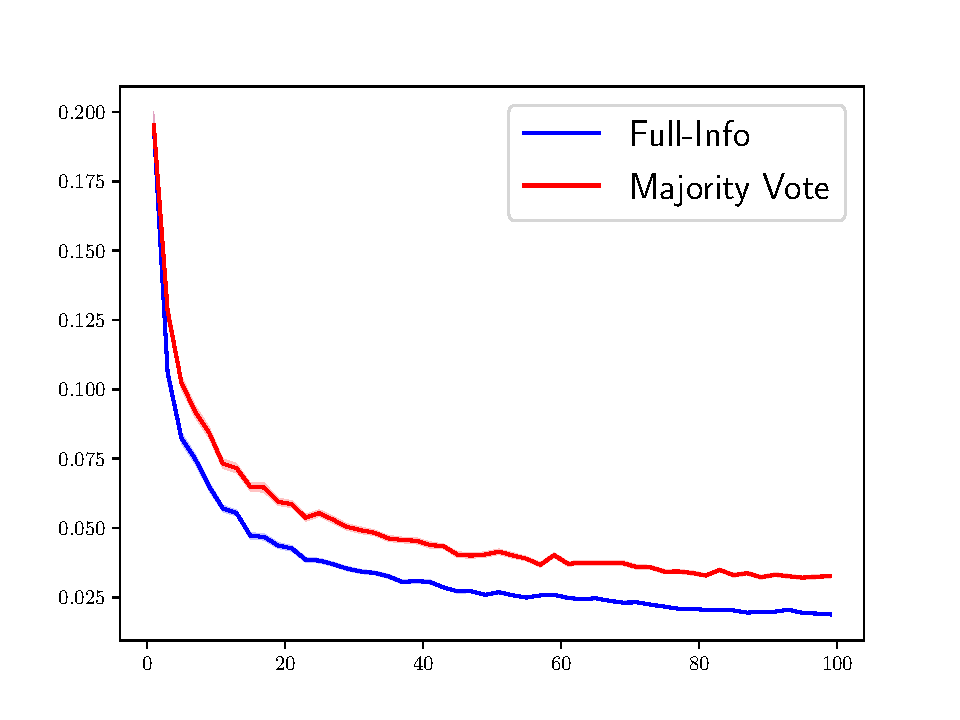
\includegraphics[width=0.3\textwidth]{figure/synthetic-class-05.pdf} &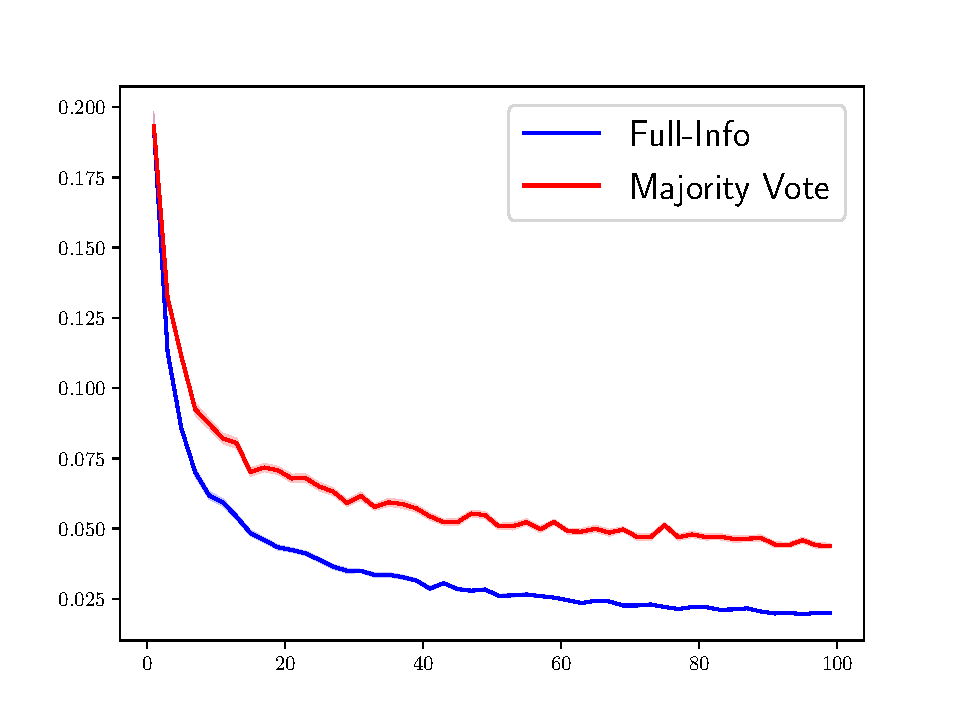
\includegraphics[width=0.3\textwidth]{figure/synthetic-class-10.pdf} &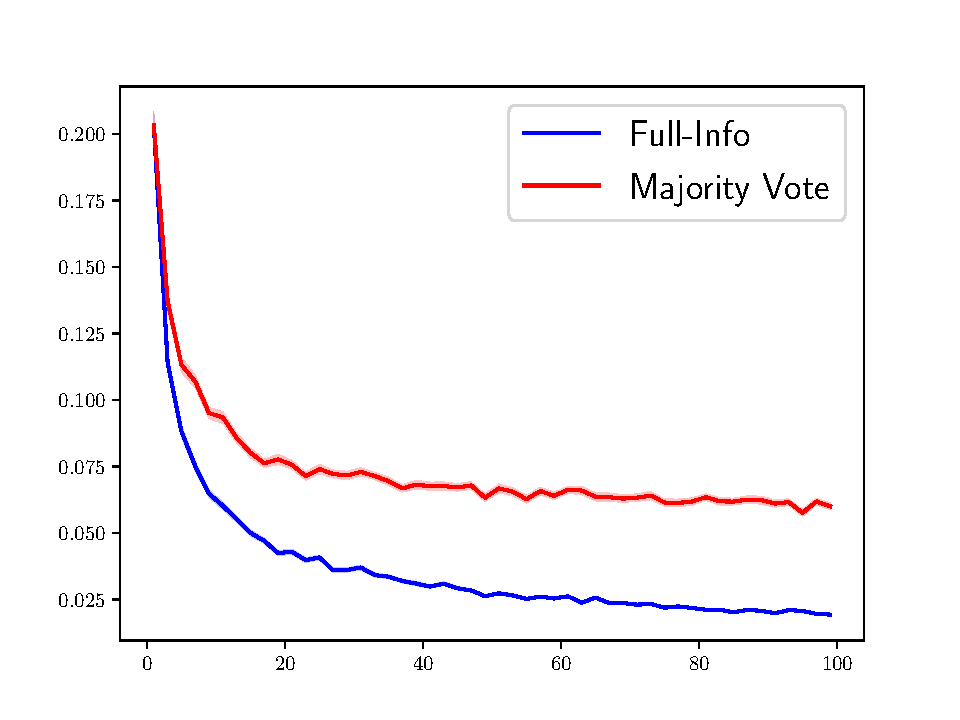
\includegraphics[width=0.3\textwidth]{figure/synthetic-class-15.pdf} \\
%% %		(a) & (b) & (c) \\
%% %		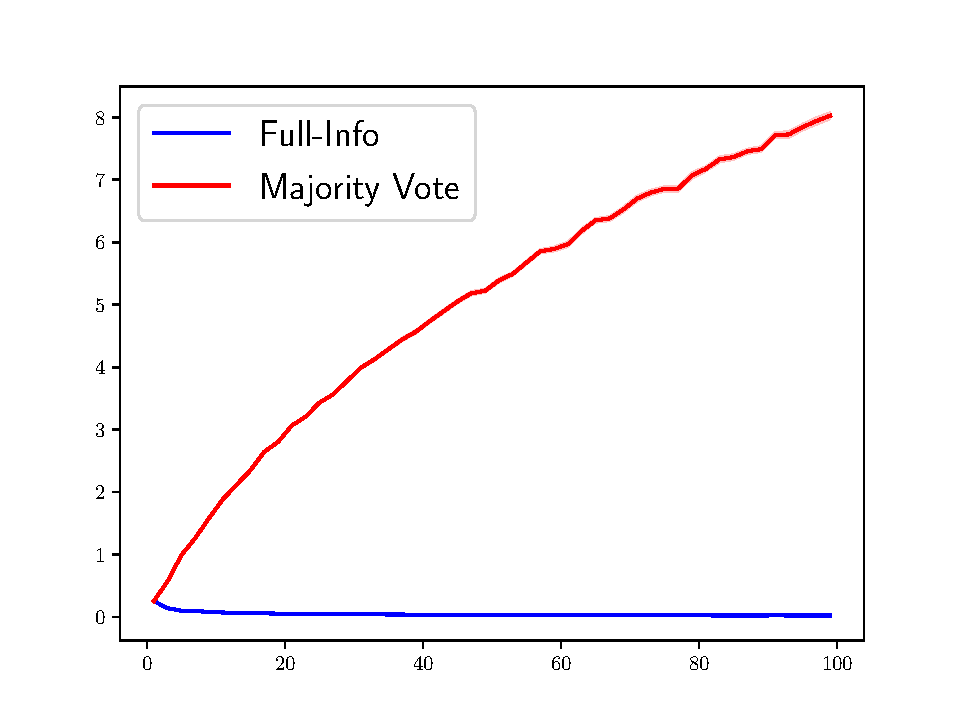
\includegraphics[width=0.3\textwidth]{figure/synthetic-calib-05.pdf} & 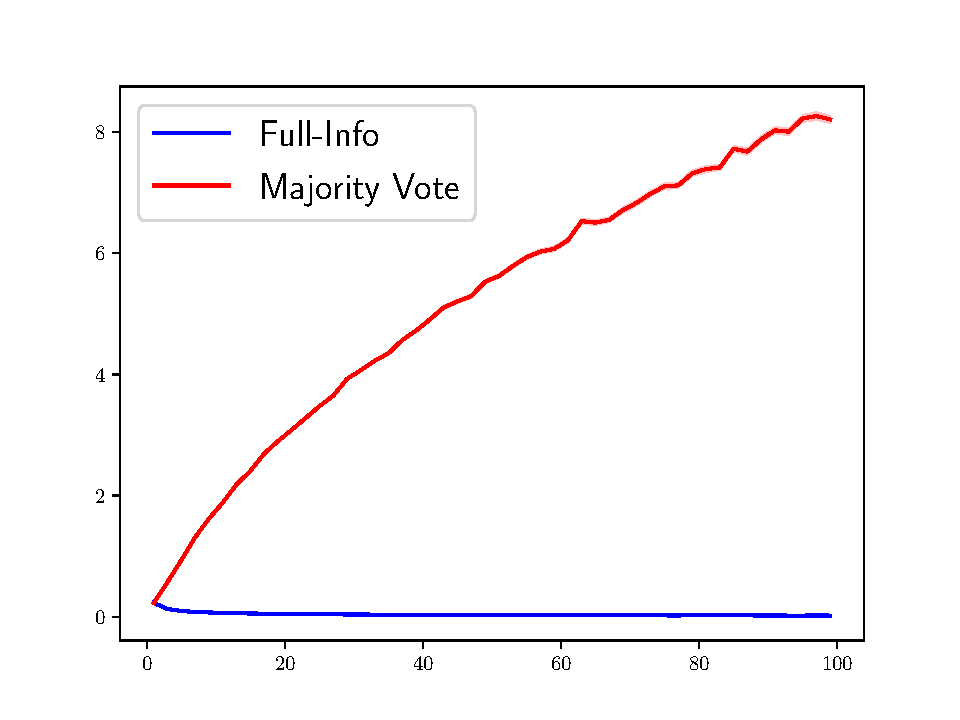
\includegraphics[width=0.3\textwidth]{figure/synthetic-calib-10.pdf} & 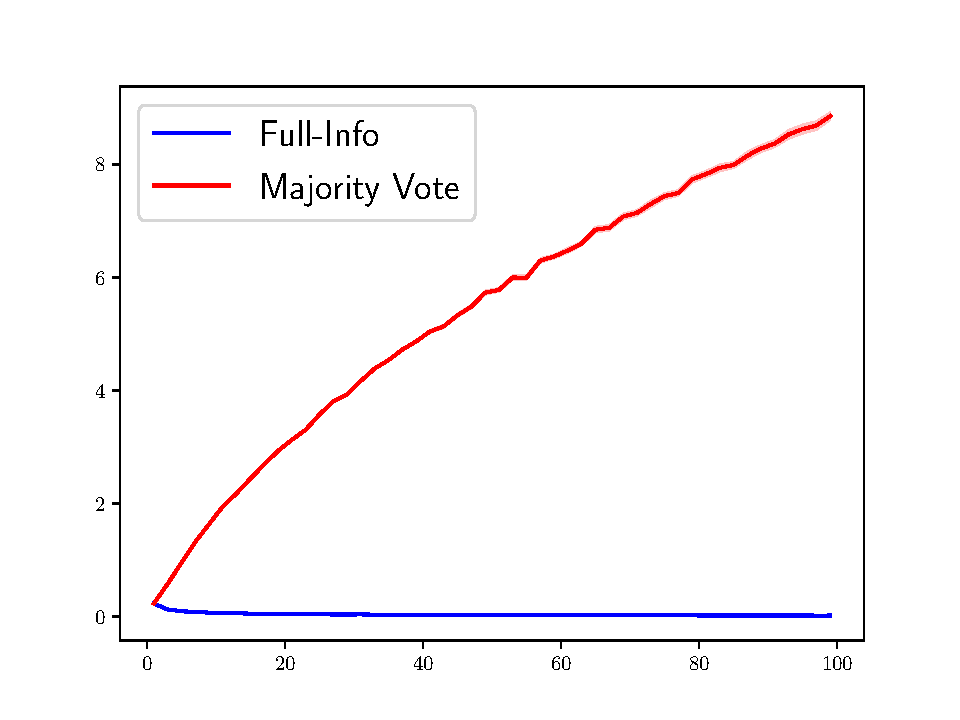
\includegraphics[width=0.3\textwidth]{figure/synthetic-calib-15.pdf}\\
%% %		(a) & (b) &  (c)
%% %	\end{tabular}
%% %	\caption{Classification error and calibration error for synthetic data for $n=1,000$ and $d=10$. For (a) $\beta = 0.5$; For (b) $\beta = 1$; For (c) $\beta = 1.5$. The errors are averaged over 100 trials with 95\% confidence bands.} \label{fig:synthetic}
%% %\end{figure}\ha{can we have only one legend in the plot?}



\subsection{BlueBirds}
\label{sec:BB}

We begin with the
\href{https://github.com/eaplatanios/noisy-labels}{BlueBirds}
dataset~\cite{WelinderBrPeBe10}, a small dataset of 108 images with ResNet features.  The task is to classify each image as one of
\textit{Indigo Bunting} or \textit{Blue Grosbeak} (two similar-looking blue
bird species). For each image, we have $39$ labels, obtained through Amazon
Mechanical Turk workers.  We use an ImageNet pretrained
ResNet50 model to generate image
features, applying PCA to reduce the dimensionality from
$d_{\textup{init}} = 2048$ to $d=25$.

We repeat the following experiment $T = 100$ times.
%
For each number $m = 1, \ldots, 35$ of labelers, we fit
the multi-label logistic model~\eqref{eq:maximum-likelihood}
and the majority vote estimator~\eqref{eq:logistic-majority},
finding calibration and classification errors using 10-fold cross validation.
%
We measure calibration error on an example $x$
by $|\logit(\wt{p}(x)) -
\logit(\what{p}(x))|$, where $\wt{p}(x)$ is the predicted probability,
$\what{p}(x)$ the empirical labeler probability,
and $\logit(p) = \log\frac{p}{1 - p}$; we measure classification
error on example $x$ with
labels $(y_1, \ldots, y_m)$ by $\frac{1}{m} \sum_{j = 1}^m \ind\{y_j \neq
\sgn(\wt{p}(x) - \half)\}$, giving an inherent noise floor because
of labeler uncertainty. We
report the results in Figure~\ref{fig:bluebird}.
These plots corroborate
our theoretical predictions: as the number of labelers $m$ increases, both
the majority vote method and the full label method exhibit improved
classification error, but considering all labels gives a (significant)
improvement in accuracy and in calibration error.

%we train the last layer of a pre-trained model \ha{which dataset for pretraining?} using the two algorithms of interest.
%
%
% \ha{why} and the images are noisy \ha{what does that mean?}.
%For each image
%The dataset was constructed by labels of 39 Amazon MTurk workers, with each of them labeling every image \textit{Indigo Bunting} or \textit{Blue Grosbeak}. For each image $i$, we generate their features $x_i \in \R^d$ by first taking the last layer outputs of a pretrained neural network $\tilde{x}_i \in \R^D$ and using PCA to reduce $\begin{bmatrix} \tilde{x}_1 & \cdots & \tilde{x}_n \end{bmatrix}^\top \in \R^{n \times D}$ to $\begin{bmatrix} x_1 & \cdots & x_n \end{bmatrix}^\top \in \R^{n \times d}$. The plots are shown in Fig.~\ref{fig:bluebird}.



\begin{figure}[ht]
  %% \vspace{-.6cm}
  \begin{center}
    \begin{tabular}{cc}
      \begin{overpic}[width=.48\columnwidth]{%,grid]{%
	  figure/resnet-class-bluebirds.pdf}
	\put(30,-1){{\small Number of labelers $m$}}
	\put(-3,20){
	  \rotatebox{90}{{\small Classification error}}}
      \end{overpic} &
      \hspace{-.3cm}
      \begin{overpic}[width=.48\columnwidth]{%,grid]{%
	  figure/resnet-calib-bluebirds.pdf}
	\put(30,-1){{\small Number of labelers $m$}}
	\put(-3,20){
	  \rotatebox{90}{{\small Calibration error}}}
      \end{overpic} \\
      (a) & (b)
    \end{tabular}
    \caption{\label{fig:bluebird} Experiments on BlueBirds dataset. (a)
      Classification error.  (b) Calibration error $|\logit(\wt{p}) -
      \logit(p)|$ with ResNet features reduced via PCA to dimension
      $d=25$. Error bars show 2 standard error confidence
      bands over $T = 100$ trials.}
  \end{center}
\end{figure}



\subsection{Crowdsourcing methods on semisynthetic CIFAR-10 labels}
\label{sec:semi-synthetic}


\newcommand{\softmax}{\textup{softmax}}

We adapt the original
CIFAR-10 dataset~\cite{KrizhevskyHi09}, which consists of 6000 $32 \times
32$ images from each of $k = 10$ classes (60,000 total images).
%
To mimic collecting messy data, rather than the single-label
in the base CIFAR-10 data, we construct pseudo-labelers
using a pretrained eighteen layer residual network
$f: \mc{X} \to \R^k$ (ResNet18~\cite{HeZhReSu16}) whose accuracy we can
adjust.
%
For $s \in \R^k$, define $\softmax(s) = [e^{s_y} /
  \sum_{l = 1}^k e^{s_l}]_{y = 1}^k$.
%
Then for an input $x \in \mc{X}$, the model outputs a score $f(x)
= {\Theta\opt}^\top \phi(x) \in \R^k$, where
$\Theta\opt = [\theta_1\opt ~ \cdots ~ \theta_k\opt] \in \R^{d \times k}$
is a matrix of per-class weights and
$\phi : \mc{X} \to \R^d$ represents the second-to-last layer
outputs of the neural network.
%
%% \in
%% \R^k$, where $\softmax(f(x))$ indicates the probabilities $\P(Y = y \mid X =
%% x)$.  The model $f$ has the form
%% \begin{equation*}
%%   f(x) = {\Theta\opt}^\top \phi(x), \qquad \text{s.t. }\Theta\opt = [\theta\opt_1 ~ \cdots ~ \theta\opt_k] \in \R^{d \times
%%   	k},
%% \end{equation*}
%% where $\Theta\opt$ is a matrix of per-class weights, and $\phi : \mc{X} \to \R^d$
%% represents the second-to-last layer outputs of the neural network. 
%
As we fit linear models, we take the outputs $\phi(x_i)$ as data, so
$X_i = \phi(x_i)$ are the covariates for the $i$th image $x_i$,
and $\Theta\opt$
is the ground-truth parameter.  We construct labels $Y_{ij}
\in \{1, \ldots, k\}$, $j = 1, \ldots, m$
by choosing the constant $\alpha > 0$
to model labeler expertise, drawing
\begin{equation*}
  \P(Y_{ij} = y \mid X_i = x)
  = \softmax(\alpha f(x))_y
  %% = \softmax(\alpha {\Theta\opt}^\top \phi(x))_y
  = \frac{\exp(\alpha \<\theta\opt_y, \phi(x)\>)}{
    \sum_{l = 1}^k \exp(\alpha \<\theta\opt_l, \phi(x)\>)}.
\end{equation*}
We vary $\alpha$ in experiments to adjust that the median value
of $p_i \defeq \max_{y \in [m]} \softmax(\alpha f(x_i))_y$, where
$p_i \in (1/k, 1)$. In the ``expert labelers'' case, we take
$\alpha \to \infty$ so that $\mbox{median}(\{p_i\}) \to 1$,
while the ``crowd labelers'' case corresponds to
$\alpha \downarrow 0$ and $\mbox{median}(\{p_i\}) \to 1/k$.

We fit $\mve$ and
$\what{\theta}^{\textup{mle}}_{n,m}$ using the multiclass logistic loss.
%
To test our predictions, we also investigate the standard
Dawid-Skene (DS)~\cite{DawidSk79} and GLAD~\cite{WhitehillWuBeMoRu09}
crowdsourcing methods.
%
The DS method models the probability that labeler $j$ assigns label $y'$
given correct label $y$ through a matrix $\alpha_j \in \R^{k \times k}$ with
$p_j(y' \mid y) = \frac{1}{1 + e^{-\alpha_j(y', y)}}$, while GLAD estimates
the probability that labeler $j$ correctly identifies the label of an
example $i$ via $p_{ij} = \frac{1}{1 + e^{-\beta_i \alpha_j}}$, where
$\alpha_j \in [-\infty,\infty]$ indicates labeler $j$'s ability and
$\beta_i \in [0, \infty]$ ambiguity in example $i$.
%
Each method uses EM to approximately maximize the likelihood $\prod_{i =
  1}^n \prod_{j = 1}^m \Prb(Y_{ij} \mid \alpha_j, \beta_i)$ (letting
$\beta_i = 1$ for DS) of the observed labels $Y_{ij}$,
initializing $\alpha$ to maximize the likelihood $\prod_{i = 1}^n \prod_{j
  = 1}^m \Prb(Y_{ij} \mid \majY_i, \alpha_j, \beta_i)$ assuming the majority
votes $\majY_i$ are correct and $\beta_i = 1$.
%
Given estimates $\what{\alpha}$ and $\what{\beta}$, one may impute soft
labels $\what{p}_i \in \R_k^+$ for each example $i$, where $\what{p}_{iy}$
indicates the method's estimated probability that example $i$ is of class
$y$, and hard labels $\what{Y}_i = \argmax_y \what{p}_{iy}$.
%
The labels yield  estimators from, respectively, hard and soft labels via
\begin{equation*}
  \what{\theta}_{\textup{h}}
  = \argmin_{\theta_1, \ldots, \theta_k}
  \sum_{i = 1}^n \log\bigg(\sum_{l = 1}^k
  e^{\<X_i, \theta_l - \theta_{\what{Y}_i}\>}\bigg)
  % \exp(\<X_i, \theta_l - \theta_{\what{Y}_i})\right)
  ~~ \mbox{and} ~~
  \what{\theta}_{\textup{s}}
  = \argmin_{\theta_1, \ldots, \theta_k}
  \sum_{i = 1}^n
  \sum_{y = 1}^k
  \what{p}_{iy} \log\bigg(\sum_{l = 1}^k
  e^{\<X_i, \theta_l - \theta_y\>} \bigg).
  % \exp(\<X_i, \theta_l - \theta_y\>\right),
\end{equation*}
We let $\dse$
and $\glade$ denote the corresponding estimators using hard labels,
and $\dspe$ and $\gladpe$ those trained with the estimated
probabilities $\what{p}_i$.
%
Our experiments use
Crowd-Kit~\citep{UstalovPaTs24}.

\begin{figure}[ht]
  %% \vspace{-.6cm}
  \begin{center}
    \begin{tabular}{cc}
      \hspace{-2cm}
      \begin{overpic}[width=.65\columnwidth]{%,grid]{%
	  figure/hard-test-error.pdf}
      \end{overpic} &
      \hspace{-2.5cm}
      \begin{overpic}[width=.65\columnwidth]{%,grid]{%
	 figure/soft-test-error.pdf}
      \end{overpic} \\
      \hspace{-2cm} (a) &
      \hspace{-2.5cm} (b) \\
      \hspace{-2cm}
      \begin{overpic}[width=.5\columnwidth]{%,grid]{%
	  figure/105.pdf}
      \end{overpic} &
      \hspace{-2.5cm}
      \begin{overpic}[width=.5\columnwidth]{%,grid]{%
	  figure/42.pdf}
      \end{overpic} \\
      \hspace{-2cm} (c) & \hspace{-2.5cm} (d)
    \end{tabular}
    \caption{\label{fig:semisynthetic} Experiments on semisynthetic
      CIFAR-10 dataset. Median labeler accuracy represents the
      median of $p_i = \max_y \softmax(\alpha f(x_i))_y$
      on the training data. Results are
      averaged over $20$ trials, and vertical axes
      give mis-classification rate from (synthetic) ground-truth labels
      on held-out test set. Legend keys correspond to
      maximum likelihood $\what{\theta}^{\textup{mle}}_{n,m}$ (MLE),
      majority vote $\mve$ (MV), hard-labeled Dawid-Skene (DS) and
      GLAD crowdsourced estimators $\dse$ and $\glade$,
      and soft-labaled Dawid-Skene (DS prob) and GLAD (GLAD prob)
      estimators $\dspe$ and $\gladpe$.
      (a) Comparison of methods using hard labels.
      (b) Comparison with crowdsourced estimated soft-labels.
      (c) Number of labelers $m$ versus test error for
      median accuracy $p = .105$ (noisy labelers). (d)
      Number of labelers $m$ versus test error for
      median accuracy $p = .4$. Both (c) and (d) report
      95\% error bars over the trials.}
  \end{center}
\end{figure}

We report the results in Fig.~\ref{fig:semisynthetic}. As we see,
when the model is well-specified,
the MLE $\what{\theta}^{\textup{mle}}_{n,m}$ %%with soft labels 
outperforms aggregation methods and black-box crowdsourcing models that
generate soft labels. Crowdsourced $\dse$ and
$\glade$ yield smaller test error than $\mve$, and using the soft labels,
$\dspe$ and $\gladpe$ further reduces the error, suggesting benefits
to using soft labels from crowdsourcing for training even if the
underlying model is unknown.

\section{Discussion and extensions}

\paragraph{Semi-parametric approaches.}
\label{sec:semi-param}
\label{sec:master-results-sem}

Our analysis separates likelihood-based approaches using all the labels, as
in~\eqref{eq:maximum-likelihood}, and majority vote estimators, which are
robust but have slower convergence, as in
Proposition~\ref{prop:lowd-misspcfd-majority-vote-m}.
%
While we mainly focus on efficiency bounds for 
procedures we view as closer to practice,
%---fitting a model based on available data---
in this section, we
present a few extensions to semiparametric approaches, more
as an amuse-bouche to motivate further efficiency investigations
rather than as a final word.
%% We thus develop a few convergence results into which we can substitute
%% semiparametric estimators.
%
In distinction from standard results in semiparametric theory
(e.g.~\cite[Ch.~25]{VanDerVaart98} or~\cite{BickelKlRiWe98}), the results
require little more than consistent estimation of the links $\sigma_j\opt$
to recover (rate optimal) $1/m$ scaling in the asymptotic covariance.

Let $\vec{\sigma} = (\sigma_1, \ldots, \sigma_m)$
be potentially distinct labeler link functions
(with $\sigma_j\opt$ denoting the true links).
Then for
$(x, y) \in \R^d \times \{\pm 1\}^m$ define the link-based loss
\begin{equation*}
  \loss_{\vec{\sigma}, \theta}(y \mid x)
  \defeq \frac{1}{m} \sum_{j = 1}^m \loss_{\sigma_j,\theta}(y_j \mid x).
\end{equation*}
%
To eliminate ambiguity in $\vec{\sigma}$,
we normalize $\ltwo{\theta\opt} = 1$,
and then define the population loss
\begin{equation*}
	L(\theta, \vec{\sigma})
	\defeq \frac{1}{m} \sum_{j = 1}^m
	\E[\loss_{\sigma_j, \theta}(Y_j \mid X)].
\end{equation*}
For the sequence $\{\vec{\sigma}_n\} \subset \fsymlinksp$
of (estimated) links and data $(X_i,
Y_i)$, $Y_i = (Y_{i1}, \ldots, Y_{im})$, we define the semi-parametric
estimator
\begin{align*}
	\spe \defeq \argmin_{\theta \in \R^d}
	\frac{1}{n} \sum_{i = 1}^n
	\loss_{\vec{\sigma}_n, \theta}(Y_i \mid X_i).
\end{align*}

Both consistency and
asymptotic normality hold under appropriate convergence of
the link functions (see Appendix~\ref{sec:semi-supp} for details).
Define the distance $d_{\flink}$ on $\R^d
\times \flink$ by
\begin{align}
  d_{\flink}\left((\theta_1, \vec{\sigma}_1), (\theta_2, \vec{\sigma}_2)
  \right)
  \defeq
  \ltwo{\theta_1 - \theta_2}
  + \LtwoPbold{\vec{\sigma}_1(-Y\<X, u\opt\>)
    - \vec{\sigma}_2(-Y\<X, u\opt\>)}.
  \label{eqn:link-distance}
\end{align}
%We make the following assumption.
%\begin{assumption}
%	\label{assumption:sp-general}
%	The links $\vec{\sigma}\opt \in \fsymlinksp$ are normalized so
%	that $\P(Y_j = y \mid X = x) = \sigma\opt_j(y \<x, u\opt\>)$, and
%	the sequence $\{\vec{\sigma}_n\} \subset \fsymlinksp$ is consistent:
%	\begin{equation*}
%		\LtwoPbold{\vec{\sigma}_n(-Y\<X, u\opt\>)
%			- \vec{\sigma}\opt(-Y\<X, u\opt\>)}
%		\cp 0.
%	\end{equation*}
%	Additionally, the mapping $(\theta, \vec{\sigma}) \mapsto
%	\nabla_\theta^2 \poploss(\theta,
%	\vec{\sigma})$ is continuous for $d_{\fsymlinksp}$ at $(u\opt,
%	\vec{\sigma}\opt)$.
%\end{assumption}
%The continuity of $\nabla_\theta^2 \poploss(\theta, \vec{\sigma})$ 
%%$\nabla_\theta^2 \poploss(\theta, \vec{\sigma})$ at
%%$(u\opt, \vec{\sigma}\opt)$ 
%allows us to develop local asymptotic normality.
%To see we may expect the assumption to hold, we give reasonably simple
%conditions sufficient for it in Lemma~\ref{lem:d-continuity-guarantees}, Appendix~\ref{sec:semi-supp}.
Then
the next master result for semi-parametric
approaches characterizes the asymptotic behavior of the
semi-parametric estimator $\spe$ using the variance function
\begin{align*}
  C_{m, \vec{\sigma}\opt} := \frac{1}{m} \cdot
  \frac{\frac{1}{m} \sum_{j = 1}^m \E[\sigma_j\opt(Z) (1 - \sigma_j\opt(Z))]}{
    (\frac{1}{m} \sum_{j = 1}^m
    \E[{\sigma_j\opt}'(Z)])^2}.
\end{align*} 
\begin{theorem}
  \label{theorem:semiparametric-master-informal}
  Let Assumption~\ref{assumption:x-decomposition} hold and assume $|Z| > 0$
  has nonzero and continuous density $p(z)$ on $(0, \infty)$.  Suppose the
  sequence $\{\vec{\sigma}_n\}$ is consistent, i.e.,
  \begin{equation*}
    \LtwoPbold{\vec{\sigma}_n(-Y\<X, u\opt\>)
      - \vec{\sigma}\opt(-Y\<X, u\opt\>)}
    \cp 0,
  \end{equation*}
  the mapping $(\theta, \vec{\sigma}) \mapsto
  \nabla_\theta^2 \poploss(\theta,
  \vec{\sigma})$ is continuous for $d_{\flink}$ at $(u\opt,
  \vec{\sigma}\opt)$, and $\Ep [\ltwo{X}^4] < \infty$.  Then $\sqrt{n}(\spe - u\opt)$ is
  asymptotically normal, and the estimator $\what{u}\sem_{n,m} =
  \spe / \ltwos{\spe}$ satisfies
  \begin{equation*}
    \sqrt{n} \prn{\what{u}\sem_{n,m} - u\opt}
    \cd \normal\prn{0, 	C_{m, \vec{\sigma}\opt}
      \prn{\proj_{u\opt}^\perp \Sigma \proj_{u\opt}^\perp}^\dagger}.
  \end{equation*}
\end{theorem}
\noindent
Notably, Theorem~\ref{theorem:semiparametric-master-informal} exhibits optimal
$1/m$ covariance scaling whenever $\E[{\sigma\opt_j}'(Z)] \gtrsim 1$.

We give two example applications of the general
theory in Appendix~\ref{sec:semi-supp}: the first analyzing a full pipeline
for a single index model setting, which robustly estimates direction $u\opt$,
the link $\sigma\opt$, and then re-estimates $\theta\opt$; the second
assuming a stylized black-box crowdsourcing mechanism that provides
estimates of labeler reliability, highlighting how even in some
crowdsourcing scenarios, there could be substantial advantages to using full
label information.

\paragraph{Future work.}

In spite of the technical detail we require to prove our results,
we view this work as almost preliminary and hope that it inspires further
work on the full pipeline of statistical machine learning,
from dataset creation to model release.
%
Many questions remain.

On the theoretical side, we focus on a stylized model of
label aggregation, with majority vote---with the exception of the
crowdsourcing model above--functioning as the
stand-in for more sophisticated aggregation strategies. It seems challenging
to show that \emph{no} aggregation strategy can work as well as multi-label
strategies; it would be interesting to delineate the benefits
and drawbacks of more sophisticated denoising.
% We
% focus throughout on low-dimensional asymptotics, using asymptotic normality
% to compare estimators. 
Additionally, the insights make low-dimensional asymptotic predictions;
investigating high-dimensional scaling might yield new perspectives
as, for, classification datasets often become
separable~\cite{CandesSu19pnas}.
%%, which is consistent with modern
%%applied machine learning~\cite{ZhangBeHaReVi21}.
%but makes the asymptotics we
% derive impossible. One option
% is to investigate the asymptotics of maximum-margin estimators,
% which coincide with the limits of ridge-regularized logistic
% regression~\cite{RossetZhHa04, SoudryHoNaGuSr18}.

On the methodological and applied side, given the extent to which the
test/challenge dataset methodology drives progress in machine
learning~\cite{Donoho17}, it seems that developing newer datasets to
incorporate labeler uncertainty could yield substantial benefits.  A
particular refrain is that modern deep learning methods are overconfident in
their predictions~\cite{GoodfellowShSz15}; perhaps by
calibrating them to \emph{labeler} uncertainty we could
improve their robustness and performance.
%
Large-scale
models now frequently use only distantly supervised
labels~\cite{RadfordKiHaRaGoAgSaAsMiClKrSu21}, making
the study of appropriate data cleaning and collection more timely.
We look forward to deeper
investigations of the foundations of the full
practice of statistical machine learning.


%\subsection*{Support}
%
%This research was partially supported by the Office of Naval Research under
%awards N00014-19-2288 and N00014-22-1-2669, the Stanford DAWN Consortium,
%and the National Science Foundation grants IIS-2006777 and HDR-1934578.

\spacingset{1.87}

\documentclass[12pt]{article}
\usepackage{amsmath}
\usepackage{bibentry}
\usepackage{graphicx}
\usepackage{booktabs}
\usepackage{multirow}
\usepackage{url} % not crucial - just used below for the URL 

%\usepackage[final]{changes}
\usepackage[draft]{changes} 
\newcommand{\stkout}[1]{\ifmmode\text{\sout{\ensuremath{#1}}}\else\sout{#1}\fi} 
\setdeletedmarkup{\stkout{#1}}

%\pdfminorversion=4
% NOTE: To produce blinded version, replace "0" with "1" below.
\newcommand{\blind}{1}

% DON'T change margins - should be 1 inch all around.
\addtolength{\oddsidemargin}{-.5in}%
\addtolength{\evensidemargin}{-1in}%
\addtolength{\textwidth}{1in}%
\addtolength{\textheight}{1.7in}%
\addtolength{\topmargin}{-1in}%

\makeatletter
\def\input@path{}
\makeatother

\usepackage{geometry}
\geometry{verbose,tmargin=1in,bmargin=1in,lmargin=1in,rmargin=1in}

\usepackage{amsmath, amssymb, amsfonts, bm, mathtools}
\usepackage{amsthm}
\usepackage{xcolor}
\definecolor{darkblue}{rgb}{0,0,.5}
\usepackage{graphicx}
\usepackage{subfigure}

\newcommand{\theHalgorithm}{\arabic{algorithm}}

\usepackage[numbers]{natbib}

\usepackage[colorlinks=true,allcolors=darkblue]{hyperref}       % hyperlinks
\usepackage{url}            % simple URL typesetting
\usepackage{booktabs}       % professional-quality tables
\usepackage{amsfonts}       % blackboard math symbols
\usepackage{nicefrac}       % compact symbols for 1/2, etc.
\usepackage{microtype}      % microtypography

\allowdisplaybreaks

\usepackage{float}
\usepackage{multirow}
\usepackage{footnote}
\usepackage{dsfont}
% \usepackage{mathabx}

\usepackage{algorithm}
\usepackage{algorithmic}
\usepackage{nicefrac}


\usepackage{hyperref}
\usepackage[capitalize]{cleveref}
\usepackage{crossreftools}


\usepackage{tikz}
\usepackage{overpic}


\definecolor{cc}{RGB}{125,0,0}
\definecolor{jd}{RGB}{0,125,0}
\definecolor{ha}{RGB}{0,0,200}

\newcommand{\cc}[1]{\textcolor{cc}{[CC: #1]}}
\newcommand{\jd}[1]{\textcolor{jd}{[JD: #1]}}
\newcommand{\ha}[1]{\textcolor{ha}{[HA: #1]}}

 % \usepackage[inline]{showlabels}


% \newcommand{\Pr}{\mathsf{Pr}}

\usepackage{dsfont}


\newcommand{\ind}{\mathds{1}}
\newcommand{\var}{\mathsf{Var}}
\newcommand{\cov}{\mathsf{Cov}}
\newcommand{\Ep}{\mathbb{E}}
\newcommand{\E}{\mathbb{E}}
\newcommand{\Prb}{\mathbb{P}}
\newcommand{\R}{\mathbb{R}} % real numbers
\newcommand{\N}{\mathbb{N}} % natural numbers
\newcommand{\Z}{\mathbb{Z}} % integers
\renewcommand{\P}{\mathbb{P}}
\newcommand{\mc}[1]{\mathcal{#1}}
\newcommand{\brc}[1]{\left\{{#1}\right\}}
\newcommand{\prn}[1]{\left({#1}\right)} % parentheses
\newcommand{\prnbig}[1]{\big({#1}\big)} % parentheses
\newcommand{\prns}[1]{({#1})} % parentheses small
\newcommand{\prnBig}[1]{\Big({#1}\Big)} % parentheses
\newcommand{\prnBigg}[1]{\Bigg({#1}\Bigg)} % parentheses
\newcommand{\brk}[1]{\left[{#1}\right]} % bracket
\newcommand{\brkbig}[1]{\big[{#1}\big]} % parentheses
\newcommand{\brkBig}[1]{\Big[{#1}\Big]} % parentheses
\newcommand{\brkBigg}[1]{\Bigg[{#1}\Bigg]} % parentheses
\newcommand{\norm}[1]{\left\|{#1}\right\|} % norm
\newcommand{\normbig}[1]{\big\|{#1}\big\|} % norm
\newcommand{\abs}[1]{\left|{#1}\right|} % norm
\newcommand{\what}[1]{\widehat{#1}}
\newcommand{\wt}[1]{\widetilde{#1}}
\newcommand{\wb}[1]{\overline{#1}}
\newcommand{\wbmj}[1]{{#1}^+}
\newcommand{\majY}{Y^+}
\newcommand{\majmark}[1]{{#1}^+}
\newcommand{\sgn}{\mathsf{sign}}
\newcommand{\pred}{\mathsf{d}}
\newcommand{\dist}{\mathsf{dist}}
\newcommand{\NN}{\mathsf{NN}}
\newcommand{\normal}{\mathsf{N}}
\newcommand{\bindist}{\mathsf{Binomial}}
\newcommand{\maj}{\mathsf{maj}}
\newcommand{\dstr}{\mathcal{P}}
\newcommand{\lr}{^{\textup{lr}}}
\newcommand{\sem}{^{\textup{sp}}}
\newcommand{\cs}{^{\textup{cs}}}
\newcommand{\mv}{^{\textup{mv}}}
\newcommand{\ds}{^{\textsc{ds}}}
\newcommand{\dsp}{^{\textsc{ds-p}}}
\newcommand{\glad}{^{\textsc{glad}}}
\newcommand{\gladp}{^{\textsc{glad-p}}}
\newcommand{\amv}{^{\textup{amv}}}
\newcommand{\mm}{^{\textup{mm}}}
\newcommand{\proj}{\mathsf{P}}
\newcommand{\proju}{\proj_{u\opt}}
\newcommand{\projperp}{\proj_{u\opt}^\perp}
\newcommand{\Flink}{\mathcal{F}_{\mathsf{link}}}
\newcommand{\lipconst}{\mathsf{L}}
\newcommand{\loss}{\ell}
\newcommand{\poploss}{L}
\newcommand{\popsignloss}{L^{\textup{sgn}}}
\newcommand{\flink}{\mathcal{F}_{\mathsf{link}}}
\newcommand{\fsymlink}{\mathcal{F}_{\mathsf{link}}^0}
\newcommand{\fsymlinkL}{\mathcal{F}_{\mathsf{link}}^{\mathsf{L}}}
\newcommand{\fsymlinksp}{\mathcal{F}_{\mathsf{link}}^{\mathsf{sp}}}
% Norms for convenience, along with sizes
\newcommand{\lone}[1]{\norm{#1}_1} % l1 norm
\newcommand{\ltwo}[1]{\norm{#1}_2} % l2 norm
\newcommand{\linf}[1]{\norm{#1}_\infty} % l-infinity norm
\newcommand{\lzero}[1]{\norm{#1}_0} % l0 norm
\newcommand{\dnorm}[1]{\norm{#1}_*} % Dual norm
\newcommand{\lfro}[1]{\left\|{#1}\right\|_{\rm Fr}} % Frobenius norm
\newcommand{\ltv}[2]{\mathsf{TV}\prn{#1, #2}}
\newcommand{\matrixnorm}[1]{\left|\!\left|\!\left|{#1}
	\right|\!\right|\!\right|} % Matrix norm with three bars
\newcommand{\normbigg}[1]{\bigg\|{#1}\bigg\|} % A norm with 1 argument and bigg
% brackets.
\newcommand{\dnormbigg}[1]{\bigg\|{#1}\bigg\|_*} % A norm with 1 argument and bigg
% brackets.
\newcommand{\lonebigg}[1]{\normbigg{#1}_1} % l1 norm
\newcommand{\ltwobigg}[1]{\normbigg{#1}_2} % l2 norm
\newcommand{\ltwobig}[1]{\normbig{#1}_2} % l2 norm
\newcommand{\ltwoBig}[1]{\normBig{#1}_2} % l2 norm
\newcommand{\linfbigg}[1]{\normbigg{#1}_\infty} % l-infinity norm
\newcommand{\norms}[1]{\|{#1}\|} % A norm with 1 argument and normal (small)
% brackets.
\newcommand{\matrixnorms}[1]{|\!|\!|{#1}|\!|\!|} % Small matrix norm
\newcommand{\matrixnormbigg}[1]{\bigg|\!\bigg|\!\bigg|{#1}\bigg|\!\bigg|\!\bigg|} % Small matrix norm
\newcommand{\lones}[1]{\norms{#1}_1} % l1 norm with small brackets
\newcommand{\ltwos}[1]{\norms{#1}_2} % l2 norm with small brackets
\newcommand{\linfs}[1]{\norms{#1}_\infty} % l-infinity norm with small brackets
\newcommand{\lzeros}[1]{\norms{#1}_0} % l0 norm with small brackets

\newcommand{\opnorm}[1]{\matrixnorm{#1}_{\rm op}} % Operator norm with three bars
\newcommand{\opnormbigg}[1]{\matrixnormbigg{#1}_{\rm op}} % Operator norm with three bars
\newcommand{\opnorms}[1]{\matrixnorms{#1}_{\rm op}} % Small operator norm with three bars
\newcommand{\<}{\langle} % Angle brackets
\renewcommand{\>}{\rangle}

\DeclareMathOperator*{\argmax}{argmax}
\DeclareMathOperator*{\argmin}{argmin}

\newcommand{\sX}{\mathcal{X}} % input space
\newcommand{\sY}{\mathcal{Y}} % output space


\newcommand{\simiid}{\stackrel{\textup{iid}}{\sim}}
\newcommand{\indic}[1]{1\!\left\{{#1}\right\}}

\newcommand{\cd}{\rightsquigarrow}
% \newcommand{\cd}{\stackrel{d}{\rightarrow}}
\newcommand{\cp}{\stackrel{p}{\rightarrow}}
\newcommand{\cas}{\stackrel{a.s.}{\rightarrow}}

\makeatletter
\long\def\@makecaption#1#2{
  \vskip 0.8ex
  \setbox\@tempboxa\hbox{\small {\bf #1:} #2}
  \parindent 1.5em  %% How can we use the global value of this???
  \dimen0=\hsize
  \advance\dimen0 by -3em
  \ifdim \wd\@tempboxa >\dimen0
  \hbox to \hsize{
    \parindent 0em
    \hfil 
    \parbox{\dimen0}{\def\baselinestretch{0.96}\small
      {\bf #1.} #2
      %%\unhbox\@tempboxa
    } 
    \hfil}
  \else \hbox to \hsize{\hfil \box\@tempboxa \hfil}
  \fi
}
\makeatother

\newcommand{\defeq}{\coloneqq}
\newcommand{\Ltwo}[1]{\norm{#1}_{L^2}}
\newcommand{\LtwoP}[1]{\norm{#1}_{L^2(\Prb)}}
\newcommand{\LtwoPbold}[1]{\norm{#1}_{L^2(\Prb)}}
\newcommand{\LtwoPn}[1]{\norm{#1}_{L^2(\Prb_n)}}
\newcommand{\LtwoPns}[1]{\norms{#1}_{L^2(\Prb_n)}}
\newcommand{\LtwoQ}[1]{\norm{#1}_{L^2(Q)}}
\newcommand{\LtwoQn}[1]{\norm{#1}_{L^2(Q_n)}}
\newcommand{\LtwoQns}[1]{\norms{#1}_{L^2(Q_n)}}
\newcommand{\lipnorm}[1]{\norm{#1}_{\textup{Lip}}}

\newcommand{\half}{\frac{1}{2}}
\newcommand{\event}{\mc{E}}

\newcommand{\conv}{\textup{Conv}}
\newcommand{\card}{\textup{card}}
\newcommand{\starhull}{\textup{Star}}
\newcommand{\hinge}[1]{\left({#1}\right)_+}
\newcommand{\hinges}[1]{({#1})_+}

\newcommand{\red}[1]{\textcolor{red}{#1}}
\newcommand{\blue}[1]{\textcolor{blue}{#1}}
\newcommand{\darkblue}[1]{\textcolor{darkblue}{#1}}

\definecolor{innerboxcolor}{rgb}{.9,.95,1}
\definecolor{outerlinecolor}{rgb}{.6,0,.2}

\newcommand{\jcdcomment}[1]{\fcolorbox{outerlinecolor}{innerboxcolor}{
    \begin{minipage}{.9\textwidth}
      \red{\bf JCD Comment:} {#1}
  \end{minipage}} \\
}

\newcommand{\opt}{^\star}
\newcommand{\subopt}{_\star}
\newcommand{\gme}{\what{\theta}_{n,m}} %General multilabel estimator
\newcommand{\tmle}{\what{\theta}\lr_{n,m}} %MLE estimator without aggregation (logistic regression)
\newcommand{\mve}{\what{\theta}\mv_{n,m}} %Majority vote estimator
\newcommand{\spe}{\what{\theta}\sem_{n,m}} %Semiparametric estimator
\newcommand{\csmle}{\what{\theta}\cs_{n,m}} %Crowdsourcing estimator
\newcommand{\dse}{\what{\theta}\ds_{n,m}} %Dawid-Skene estimator
\newcommand{\dspe}{\what{\theta}\dsp_{n,m}} %Dawid-Skene soft estimator
\newcommand{\glade}{\what{\theta}\glad_{n,m}} %GLAD estimator
\newcommand{\gladpe}{\what{\theta}\gladp_{n,m}} %GLAD soft estimator
\newcommand{\G}{\mathbb{G}}


% \usepackage{enumerate}
\usepackage{enumitem}

\newtheorem{claim}{Claim}[section]
\newtheorem{lemma}[claim]{Lemma}
\newtheorem{assumption}{Assumption}
\newtheorem{definition}{Definition}
\newtheorem{theorem}{Theorem}
\newtheorem{example}{Example}
\newtheorem{proposition}{Proposition}
\newtheorem{remark}{Remark}
\newtheorem{corollary}{Corollary}
\renewcommand{\theassumption}{A\arabic{assumption}}
\renewcommand{\bindist}{\mathsf{Bin}}

\usepackage{xr}
\externaldocument{JASA-supp}

\begin{document}

%\bibliographystyle{natbib}

\def\spacingset#1{\renewcommand{\baselinestretch}%
{#1}\small\normalsize} \spacingset{1}

%%%%%%%%%%%%%%%%%%%%%%%%%%%%%%%%%%%%%%%%%%%%%%%%%%%%%%%%%%%%%%%%%%%%%%%%%%%%%%

\if1\blind
{
  \title{\bf How many labelers do you have? \\
  	A closer look at gold-standard labels}
  \author{Chen Cheng\thanks{Department of Statistics, Stanford University; email: \texttt{chencheng@stanford.edu}.} \and
  	Hilal Asi\thanks{Department of Electrical Engineering, Stanford University; email: \texttt{asi@stanford.edu}.}
  	\and
  	John Duchi\thanks{Departments of Statistics and Electrical Engineering, Stanford University; email: \texttt{jduchi@stanford.edu}.}}
  \maketitle
} \fi

\if0\blind
{
  \bigskip
  \bigskip
  \bigskip
  \begin{center}
    {\LARGE\bf How many labelers do you have? \\
    	A closer look at gold-standard labels}
\end{center}
  \medskip
} \fi

\bigskip

% -*- mode: latex -*- %

\begin{abstract}
  The construction of most supervised learning datasets revolves around
  collecting multiple labels for each instance, then aggregating the labels
  to form a type of ``true'' label.
  %
  We question the wisdom of this pipeline by developing a (stylized)
  theoretical model of this process and analyzing its statistical
  consequences, showing how access to non-aggregated label information can
  make training well-calibrated models more feasible than it is with
  cleaned labels.
  %
  The entire story, however, is subtle, and the
  contrasts between aggregated and fuller label information depend on
  the particulars of the problem,
  where estimators that use aggregated information exhibit robust but slower
  rates of convergence, while estimators that can effectively
  leverage all labels converge more quickly \emph{if} they have
  fidelity to (or can learn) the true labeling process.
  The theory
  makes several predictions for real-world datasets, including when
  non-aggregate labels should improve learning performance, which we
  test to corroborate the validity of our predictions.
\end{abstract}


\noindent%
{\it Keywords:} Label aggregation, classification and calibration, crowdsourcing
\vfill

\newpage
\spacingset{1.87} % DON'T change the spacing!

% -*- Mode: latex -*- %

\section{Introduction}

Challenge datasets drive advances in statistical machine
learning~\cite{MarcusSaMa94, LewisYaRoLi04, AsuncionNe07, KrizhevskyHi09,
  DengDoSoLiLiFe09, RussakovskyDeSuKrSaMaHuKaKhBeBeFe15},
making the collection of
labeled data essential~\cite{Donoho17}.
%
While in the past, experts could label reasonably sized datasets, the cost
and size of modern datasets often precludes such annotation, motivating
crowdsourcing and other dataset generation strategies that aggregate
non-expert and expert feedback~\citep{DawidSk79,
  WhitehillWuBeMoRu09, RussakovskyDeSuKrSaMaHuKaKhBeBeFe15,
  CodellaRoTsCeDuGuHeKaLiMa19, GadreEtAl23}.
%% SchuhmannBeVeGoWiChCoKaMuWoScKuCrScKaJi22,
%
Frequently, published data contain aggregated label information; for
example, in the dataset~\cite{CodellaRoTsCeDuGuHeKaLiMa19}
%% RotembergKuBeCaChCoCoDuGuGu21}
of skin lesion images to be classified as
malignant, biopsy and histology confirm positive examples, while physician
consensus determines negative examples, yet the published data includes no
notion of disagreement or uncertainty in these consensuses.
%
Similarly, the benchmark CIFAR~\citep{KrizhevskyHi09} and
ImageNet~\citep{DengDoSoLiLiFe09, RussakovskyDeSuKrSaMaHuKaKhBeBeFe15}
computer vision challenges include only a single label for each example, in
spite of deriving from multiple pieces of feedback per image.
%
Researchers typically perform such aggregation in effort to obtain
``high-quality'' or ``true'' labels~\cite{DengDoSoLiLiFe09,
  RussakovskyDeSuKrSaMaHuKaKhBeBeFe15, DawidSk79,
  WhitehillWuBeMoRu09}.

Yet most statistical machine learning development does not investigate this
full data generating process, assuming only that data comes in the form of
$(X, Y)$ pairs of covariates $X$ and labels $Y$~\cite{Vapnik95,
  BoucheronBoLu05, BartlettJoMc06, HastieTiFr09}.
%
We argue for a more
holistic perspective: that analysis and algorithmic development should focus
on the complete statistical learning pipeline, from dataset construction to
model output.
%
We question the extent to which such label cleaning strategies are
essential, arguing that benchmark datasets ought to include noisy labels as
a rule; one may always clean the data in subsequent stages, but sometimes
the more nauced labeling information may yield more accurate downstream
models.

%\cc{Also the second perspective---the crowdsourcing community aims to obtaining labels as clean as possible but largely ignoring how it would affect downstream tasks, or simply assuming the goal is to clean the labels as much as possible. Our results suggest (i) maybe the correct upstream tasks is not to get gold-standard labels; (ii) provided we can get multilabeled data from upstream tasks, we essentially have a different statistical learning model from the classical ones which makes it possible for us to do more.} 

%% We revisit this data generation process and question its aggregation
%% strategies.  While it is tempting to apply majority-vote aggregation to
%% obtain an expert label, resembling a typical machine learning dataset, this
%% ignores the inherent uncertainty and noise in this pipeline.  There has been
%% numerous amounts of work from the crowd-sourcing
%% community~\cite{WhitehillWuBeMoRu09,WelinderBrPeBe10,TianZh15} (see
%% Section~\ref{sec:related-work} for more details) that \emph{experimentally}
%% study the above process and design better algorithms by taking into
%% consideration the inherent noise in the labels. However, a complete
%% (theoretical) understanding of this process and the effects of uncertainties
%% and other important problem parameters---such as number of labelers and data
%% noise---is still lacking.

We develop a stylized theoretical model to capture uncertainty in the
labeling process, allowing us to understand the limitations of and possible
improvements to using aggregated data in a statistical learning pipeline.
%
We model each example as a pair $(X_i, (Y_{i1},\dots,Y_{im}))$ where $X_i$
is a data point and $Y_{ij}$ are noisy binary labels.
%
The basic
formulation of our results compares two methods: empirical risk
minimization using all labels and empirical risk minimization using
majority vote labels $\majY$.
%
While this oversimplifies label
aggregation strategies~\cite{DawidSk79, RussakovskyDeSuKrSaMaHuKaKhBeBeFe15,
  RatnerBaEhFrWuRe17},
the simplicity (i) allows us to understand
fundamental limitations of algorithms based on majority-vote aggregation,
(ii) facilitates circumventing these limits via non-aggregated
information, and (iii) provides a base for future work: the purposeful
simplicity permits classical tools to apply.
%
In these models, our results show that estimators using non-aggregated labels
outperform those that use aggregated (majority-vote)
labels if the predictive model has fidelity to the data,
majority-vote estimators provide robust (but slower) convergence, and these
tradeoffs are fundamental.
%
We extend the results to include misspecification, semiparametric
scenarios, and simple models of learned annotator reliability.

While our models are stylized, they make testable predictions for real data
beyond simplified scenarios, in particular, that models fit on
non-aggregated data should both make better-calibrated predictions and have
lower classification error than those using cleaned labels.
%
Experiments on two real and one large semisynthetic dataset corroborate the
implications of our theory beyond logistic models: majority-vote-based
algorithms yield uncalibrated predictors, while algorithms using full label
information provide (more) calibrated predictors.
%
The former algorithms exhibit worse classification error in our experiments,
with the error gap depending on parameters---e.g.,
noise---we address in our theoretical models.
 

\subsection{Problem formulation}
\label{sec:formulation}

%% To situate our results, we begin by
%% providing the key ingredients in the paper.

% \paragraph{The label model.}
Consider covariates $X_i \simiid \P_X$, $X_i \in \R^d$, in a
binary classification problem with $m$ labelers,
who annotate points independently through a generalized linear
model (GLM) via link functions %% $ \flink$, where
\begin{align*}
  \sigma_1\opt, \dots,
  \sigma_m\opt \in \flink := \brc{\sigma : \R \to [0, 1]
    \mid \sigma(0) = 1/2, \sgn(\sigma(t) - 1/2) = \sgn(t)}.
\end{align*} 
%% Here $\sgn(t) = -1$ for $t <0$, $\sgn(t) = 1$ for $t > 0$ and $\sgn(0) = 0$. 
For example, in the logistic model where
labelers have identical link, $\sigma_j\opt(t) = 1 / \prn{1 + e^{-t}}$.
%
If $\sigma(t) + \sigma(-t) = 1$ for all $t \in \mathbb{R}$, we say the
link function is symmetric, denoting the class of symmetric
links by $\fsymlink \subset \flink$.
%
Labels then follow the distribution
\begin{align}
  \Prb_{\sigma, \theta}(Y = y \mid X = x) & =
  \sigma ( y \< \theta, x\>) ~~~ \mbox{for~} y \in \left\{\pm 1\right\},
  ~ x,\theta \in \R^d. \label{eq:general-calibration-model}
\end{align}
Key to our model, and what allows our analysis, is that we assume
labelers use the same linear classifier $\theta\opt \in \R^d$, %%---though each
%%labeler $j$ may have a distinct link $\sigma_j\opt$---
so we obtain conditionally independent labels $Y_{ij} \sim \Prb_{\sigma_j\opt,
  \theta\opt}(\cdot \mid X_i)$.
 We
seek to recover $\theta\opt$ or the direction $u\opt := \theta\opt /
\ltwo{\theta\opt}$ from the observations $(X_i, Y_{ij})$.

\paragraph{Error measures.}
We evaluate an estimator $\what{\theta}$ and associated direction $\what{u}
\defeq \what{\theta} / \ltwos{\what{\theta}}$ through
\begin{enumerate}[leftmargin=10em,label=(\textsc{E}.\roman*)]
\item \label{item:class}
  The classification error: $\ltwos{u\opt - \what{u}}
  = \sqrt{2(1 - \<u\opt, \what{u}\>)}$.
  % \tag{\textsc{E.class}
\item \label{item:cal}
  The calibration error:~~ $\ltwos{\theta\opt - \what{\theta}}$.
\end{enumerate}
%% \begin{align*}
%%   \textbf{(i)} & \quad \text{The classification error:} ~~ ~\|u^\star - \what{u}\|_2 = \sqrt{2(1 - \langle u\opt, \what{u} \rangle)}. \\
%%   \textbf{(ii)} & \quad
%%   \text{} ~~~~ ~~ \|\theta^\star - \what{\theta}\|_2.
%% \end{align*}
To motivate these errors, note that for classification, we only need to
control the difference between the directions $\what{u}$ and $u\opt$, while
calibration---that for a data point $X$, the value $\sigma_j\opt( \<
\what{\theta}, X \>)\approx \sigma_j\opt(\< \theta\opt, X \>)$---requires
controlling the error in $\what{\theta}$ as an estimate of $\theta\opt$.
%
If $X$ is rotationally symmetric,
then $\P(\sgn(\<X, u\>) \neq \sgn(\<X, u\opt\>)) = \frac{1}{\pi}
\cos^{-1}\<u, u\opt\>$ for any unit vectors $u, u\opt$; because $\cos^{-1} t
= (1 + o(1)) \sqrt{2(1 - t)}$ as $t \uparrow 1$, the classification
error~\ref{item:class}, $\ltwo{u\opt - u} =
\sqrt{2(1 - \<u, u\opt\>)}$, is asymptotically equivalent to the angle
between $u$ and $u\opt$.

\paragraph{Estimators.}
We consider two types of estimators: one
using processed labels $\majY_i$ for each
example $X_i$, and the other
using each label $Y_{i1}, \ldots, Y_{im}$.
%
To center discussion, we instantiate this temporarily via logistic
regression for the logistic link $\sigma\lr(t) = \frac{1}{1 + e^{-t}}$,
defining
\begin{align*}
  \loss_\theta\lr(y \mid x) = -\log \Prb_{\sigma\lr, \theta}(y \mid x)
  = \log(1 + e^{-y\<x,\theta\>})  .
\end{align*}
In the non-aggregated model, we let let $\Prb_{n,m}$ be the empirical
measure on $\{(X_i, (Y_{i1},\dots,Y_{im}))\}$ and consider the logistic
regression estimator (i.e., the MLE assuming the logistic model)
\begin{align}
  \label{eq:maximum-likelihood}
  \tmle = \argmin_\theta \left\{\Prb_{n,m} \loss_\theta\lr
  = \frac{1}{nm} \sum_{i = 1}^n \sum_{j = 1}^m \loss_\theta\lr(Y_{ij} \mid X_i)
  \right\}.
\end{align}
We focus on the simplest
aggregation strategy, where example $i$ has majority vote label
\begin{align*}
  \majY_i = \maj(Y_{i1}, \ldots, Y_{im})
  \defeq \sgn\left(\sum_{j=1}^m Y_{ij}\right)
  ~~~\mbox{where}~~~
  \sgn(0) \sim \mathsf{Ber}(1/2)
\end{align*}
%% (breaking ties randomly).
Then letting $\majmark{\Prb}_{n,m}$ be the empirical measure on
$\{(X_i, \majY_i)\}$, the majority-vote estimator solves
\begin{align}
  \label{eq:logistic-majority}
  \mve = \argmin_\theta  \brc{\majmark{\Prb}_{n,m}\loss_\theta\lr = \frac 1 n \sum_{i=1}^n  \loss_\theta\lr(\majY_i \mid X_i)}.
\end{align}
Method~\eqref{eq:logistic-majority} acts as our proxy for the ``standard''
data analysis pipeline, with cleaned labels, while
method~\eqref{eq:maximum-likelihood} is our proxy for non-aggregated methods
using all labels.
%
More general formulations than the majority
vote~\eqref{eq:logistic-majority} could allow complex aggregation
strategies, e.g., crowdsourcing, but we simplify to capture what we view as
the essentiae for problems (e.g.\ CIFAR~\cite{KrizhevskyHi09} or
ImageNet~\cite{RussakovskyDeSuKrSaMaHuKaKhBeBeFe15}) where only aggregated
label information is available.

Our main results characterize the
asymptotics of the
estimators $\mve$ and $\tmle$.
%
Under
appropriate assumptions on the data generating
mechanisms~\eqref{eq:general-calibration-model}, which include
misspecification, we (i) provide consistency results that elucidate the
limits for $\mve$, $\tmle$, and a few more general
estimators, and (ii) evaluate their limit distributions via
asymptotic normality. The latter allows comparison
of the estimators through their limiting covariances, which
exhibit (to us) interestingly varying dependence on $m$ and the scaling of
the true parameter $\theta\opt$.

\subsection{Summary of results and implications}

Asymptotic characterization of the
estimators~\eqref{eq:maximum-likelihood}--\eqref{eq:logistic-majority}
provides our main avenue to highlighting the import of multiple labels.
%
Table~\ref{table:comparisons}  summarizes our results, comparing
the performance of the MLE-type~\eqref{eq:maximum-likelihood} and
majority vote~\eqref{eq:logistic-majority} estimators for the
classification~\ref{item:class} and calibration~\ref{item:cal} errors.
%
We highlight estimator performance in two scenarios:
``single link'' corresponds to the case that the loss is
well-specified, while ``mis-specified''
corresponds to the case that $\loss_\theta(y \mid x) \neq -\log
\Prb_{\sigma,\theta}(y \mid x)$, which may occur when labelers have
distinct link functions $\sigma$ or the model is incorrect.
%
In all cases, the
estimate $\what{\theta}$ and
vector $\what{u} = \what{\theta} / \ltwos{\what{\theta}}$
are asymptotically normal around a scalar multiple of $\theta\opt$,
with differeing scaling and asymptotic variance.
%
With $m$ labelers,
each estimator yields a rate $r(m)$ and scale $t(m)$ for which
\begin{align}
  \label{eqn:limit-scaling-for-table}
  \sqrt{n}(\what{u} - u\opt)
  \cd \normal(0, r(m) \Sigma_{\textup{n}})
  ~~~ \mbox{and} ~~~
  \sqrt{n}(\what{\theta} - t(m) \theta\opt)
  \cd \normal(0, \Sigma_{\textup{u}}),
\end{align}
where $\Sigma_{\textup{n}}$ and $\Sigma_{\textup{u}}$ are ``normalized'' and
``unnormalized'' covariances, respectively.
%
The classification error~\ref{item:class} is small whenever $r(m) \ll 1$,
while the calibration error~\ref{item:cal} is small when $t(m) \approx 1$,
and Table~\ref{table:comparisons} shows the
scalings~\eqref{eqn:limit-scaling-for-table} for the different estimators.

\begin{table}
  \centering
  \begin{tabular}{c|c|c}
    \toprule 
    & MLE-type estimator~\eqref{eq:maximum-likelihood}
    & majority-vote estimator~\eqref{eq:logistic-majority} \\
    \hline
    single link
    & \textbf{Classification}:
    $r(m) \asymp \frac{1}{m}$
    & Classification: $r(m) \asymp \frac{1}{\sqrt{m}}$ \\
    (well-specified) & \textbf{Calibration}:
    $t(m) = 1$ &
    Calibration: $t(m) \asymp \sqrt{m}$ \\ 
    \hline
    mis-specified or
    & Calibration: $t(m) \asymp 1$ &  Calibration: $t(m) \asymp \sqrt{m}$  \\ 
    multiple links & Classification: $r(m) \asymp 1$ &
    \textbf{Classification}: $r(m) \asymp 1 / \sqrt{m}$
    \\
    \hline
  \end{tabular}
  \caption{
    Comparison of multi-label and majority-vote estimators
    for $X \sim \normal(0, I_d)$
    according to the scalings in classification error
    $r(m)$ and calibration error $t(m)$ that
    the limits~\eqref{eqn:limit-scaling-for-table} identify.
    %
    If $t(m) \gg 1$, the model is uncalibrated; if the rate $r(m)$ is small,
    the model achieves lower asymptotic variance.
    %
    Boldface indicates the associated estimator
    is (rate) optimal. \label{table:comparisons}}
\end{table}

%% We obtain several results clarifying the distinctions between
%% estimators that use aggregate labels from those that treat them
%% individually.

\paragraph{Improved performance using multiple labels for well-specified models}
%% As in our discussion above,
We begin in Section~\ref{sec:well-sepcified-mod} by specializing our main
results to the logistic model.
%
We show that the MLE~\eqref{eq:maximum-likelihood} is
calibrated and enjoys faster rates of convergence (in $m$) than the
majority-vote estimator~\eqref{eq:logistic-majority}.
%
The improvements depend on the underlying distribution, and
Propositions~\ref{prop:lowd-maximum-likelihood}
and~\ref{prop:lowd-majority-vote-m-noise} connect them to
Mammen-Tsybakov-type noise conditions.
%
In ``standard'' cases, the improvement scales as
$\sqrt{m}$; for problems with little classification noise, the majority vote
estimator becomes brittle (relatively slower), while the convergence rate
gap decreases for noisier problems.


\paragraph{Robustness of majority-vote estimators}
Our results also evidence support for majority vote
estimators~\eqref{eq:logistic-majority}.  Section~\ref{sec:mis-spec}
provides master results holding for well- and mis-specified losses, which
highlight the robustness of the majority vote estimator
(cf.\ Table~\ref{table:comparisons}).
%
The faster rates MLE-type estimators~\eqref{eq:maximum-likelihood} enjoy
when the model is correct break down in ways we make precise for
mis-specified models; in contrast, majority-vote-type
estimators~\eqref{eq:logistic-majority} maintain their (not quite optimal)
improved convergence guarantees, even under mis-specification, suggesting
practical value to cleaning data when correctly modeling uncertainty is
impossible.

\paragraph{Fundamental limits of majority vote}
Via local asymptotic minimax theory, Section~\ref{sec:lower-bound} develops
fundamental limits for estimation given only majority vote labels $(X,
\majY)$, which coincide with our results in
Section~\ref{sec:well-sepcified-mod}.
%
These results highlight how cleaned labels force slower
convergence in the number of labelers $m$ while reinforcing the claims of
robustness.
%
In particular, while a mis-specified link function introduces structural
bias that MLE-type estimators using all labels cannot overcome, majority
vote-based estimators achieve rate-optimal convergence for procedures
receiving cleaned labels $\majY$ (making the rate $r(m)$ in the bottom right
of Table~\ref{table:comparisons} sharp).

%% In particular, in both unspecified and well-specified cases, we cannot
%% achieve calibration---contrasting with non-aggregated data, which allows
%% calibrated estimators.

%with the simple result that any
%estimator based on majority vote aggregation cannot be calibrated:
%there exist distributions with distinct numbers of labelers $m$
%and link functions $\sigma$ that induce identical joint distributions on
%$(X, \majY)$.  This contrasts with non-aggregated data, which allows
%calibrated estimators.

%% (\Cref{sec:mis-spec}) we study the mis-specified model where the estimators
%% use a logistic model for the labelers which follow a different
%% model. Somewhat surprisingly, our results demonstrate that the majority vote
%% estimator is more robust to model mis-specification. In particular, it can
%% provide faster convergence rates than the multi-label estimator by a factor
%% of $\sqrt{m}$.

\paragraph{Experimental evaluation}
Our theoretical results predict two outcomes: (i) \emph{if} the
model has fidelity to the labeling process, then using all noisy labels
should yield better estimates than procedures using cleaned labels, and
(ii), that majority vote estimators should be more robust. In
Section~\ref{sec:experiments}, we thus provide real and semi-synthetic
experiments that corroborate the theoretical predictions; the experiments
also highlight a need, which some researchers are now beginning to
address~\cite{GadreEtAl23}, for more applied dataset development so that we
can evaluate the consequences of filtering and otherwise manipulating the
data we use.

\paragraph{Semi-parametric approaches}
%% The final theoretical component of the paper (Section~\ref{sec:semi-param})
%% provides an exemplar approach that puts the pieces together to achieve
%% efficiency via semi-parametric approaches. 
In our discussion (Section~\ref{sec:semi-param}), we include an exemplar
approach for estimation via semi-parametric approaches, where
one estimates labelers' links and reliability.
%
While not our main focus, the results provide potential insights into
estimation using existing crowdsourcing techniques, where black box
algorithms provide measures of labeler reliability that one may incorporate
to achieve rate-optimal estimation.


\subsection{Related work}
\label{sec:related-work}

%% We briefly overview related work, acknowledging that 
To make our theoretical model tractable, we capture only a few of the complexities inherent in
dataset construction. Label aggregation strategies often attempt to
evaluate labeler uncertainty, dating to~\citet{DawidSk79}, who study
labeler uncertainty estimation to overcome noise in
clinical patient measurements. With the rise of
crowdsourcing, such reliability models have
attracted interest, with approaches for optimal budget
allocation~\cite{KargerOhSh14}, addressing untrustworthy or malicious
labelers~\cite{CharikarStVa17}, and more broadly a line of applied~\cite{DengDoSoLiLiFe09, RussakovskyDeSuKrSaMaHuKaKhBeBeFe15} and theoretical work
studying crowd labeling and aggregation~\cite{WhitehillWuBeMoRu09,
  WelinderBrPeBe10, RatnerBaEhFrWuRe17}.
%%, with substantial
%% applications~\cite{DengDoSoLiLiFe09, RussakovskyDeSuKrSaMaHuKaKhBeBeFe15}.

Many of these focus, however, on obtaining a single
trustworthy label for each example. Our work takes a
different perspective.  First, we target statistical analysis for
the full learning pipeline---understanding the landscape of the
learning problem with multiple labels for each example---as opposed to
obtaining only clean labels. Moreover, we argue for
calibrating the resulting predictive model, which cleaned
labels necessarily impede. We therefore adopt a perspective similar to
the applied works~\citep{PetersonBaGrRu19,PlataniosAlXiMi20},
which highlight how incorporating human
uncertainty into learning pipelines can make classification ``more
robust''~\citep{PetersonBaGrRu19}.  Instead of splitting the learning
procedure into two phases, where the first aggregates labels and the second
trains, we use non-aggregated labels throughout
learning. \citet{PlataniosAlXiMi20} directly
model labeler reliability via a richer model than our stylized
scenarios, but our
approach allows theoretically precise description of the
methods' limiting
behavior.


Our results complement a growing body of work in machine learning.
%
The Neural Information Processing Systems conference
includes a Datasets and Benchmarks track, as they
``are crucial for the development of machine learning
methods''~\cite{BeygelzimerLiVaDa21},
%
%% As a particular examplar, \citet{GadreEtAl23} introduce DataComp,
%% a testbed for experimental work on datasets,
building off the long history
of dataset-driven development in machine learning~\cite{HardtRe22}.
%
We attempt to lay statistical foundations for this line of work.

%We mention in passing that our consistency results rely on
%distributional assumptions on the covariates $X$, for example,
%Gaussianity. That such technical conditions appear may be familiar from work,
%for example, in single-index or nonlinear measurement models~\cite{PlanVe16,
%  PlanVe13}. In such settings, one assumes $\E[Y \mid X] = f(\<\theta\opt,
%X\>)$ for an unknown increasing $f$, and it is essential that $\E[Y X]
%\propto \theta\opt$ to allow estimation of $\theta\opt$; we leverage similar
%techniques.

\paragraph{Notation}
For a matrix $M$, $\norm{M}$ denotes its spectral norm and $M^\dagger$ its
Moore-Penrose pseudo inverse.
%
For a unit vector $u$, $\proj_{u}^\perp \defeq
I - u u^\top$ projects to the space orthogonal to $\mathrm{span}\{u\}$.
%
We use the empirical process notation $\Prb Z = \int z d\Prb(z)$ and $\cd$
denotes convergence in distribution.
%
We write $f(x) \asymp g(x)$ for $x \in \R_+$ if there exist
numerical constants $0 < c_1, c_2 < \infty$ and $x_0 \geq 0$ such that $c_1
|g(x)| \leq |f(x)| \leq c_2|g(x)|$ for $x \geq x_0$,
and
$c = o_m(1)$ means $c \to 0$ as $m \to \infty$.


\section{The well-specified logistic model}\label{sec:well-sepcified-mod}

We begin in a setting that allows the cleanest and most precise comparisons
between a method using aggregated labels~\eqref{eq:logistic-majority} and
one without~\eqref{eq:maximum-likelihood} by considering the logistic link
for~\eqref{eq:general-calibration-model},
\begin{align*}
  \sigma\lr(t) = \frac{1}{1 + e^{-t}} \in \fsymlink.
\end{align*}
%This simplicity allows results that highlight many of the conclusions we
%draw, and so we present initial, relatively clean, results for the
%estimators~\eqref{eq:maximum-likelihood} and~\eqref{eq:logistic-majority}
%here.  
In particular, we assume identical links $\sigma_1\opt = \dots =
\sigma_m\opt = \sigma\lr$ and an i.i.d.\ sample $X_1, \ldots, X_n$, where
for each $i \in [n]$ we draw $(Y_{i1}, \ldots, Y_{im}) \simiid
\Prb_{\sigma\lr,\theta\opt}(\cdot \mid X_i)$ for a true vector $\theta\opt$.


\subsection{The isotropic Gaussian case} \label{sec:gauss}

To deliver the general taste of our results on the performance of the full
information~\eqref{eq:maximum-likelihood} and majority
vote~\eqref{eq:logistic-majority} approaches, we start by studying the
simplest case when $X \sim \normal(0, I_d)$.

\paragraph{Performance with non-aggregated data.}

The
non-aggregated MLE $\tmle$ in Eq.~\eqref{eq:maximum-likelihood}
admits a standard analysis,
which we state as a corollary of
Proposition~\ref{prop:lowd-maximum-likelihood} to come.
%
%Let the population log loss be $L(\theta) = \Prb \loss_\theta(Y \mid X)$. When $m$ is fixed, we can view $(X_i, Y_{i1}, \cdots, Y_{im})$ as independent samples from $\R^d \times \left\{\pm 1\right\}^m$ which allows us to directly employ the standard asymptotic normality for maximum likelihood estimators. Let $\what{u}\lr_{n,m}$ be the normalized version of $\what{\theta}\lr_{n,m}$. The classical theory tells us the following.
\begin{corollary}
  \label{cor:lowd-maximum-likelihood-Gaussian} 
  Let $X \sim \normal(0, I_d)$ and $t\opt = \ltwos{\theta\opt}$. The maximum
  likelihood estimator $\tmle$ is consistent, with $\tmle \cp
  \theta\opt$, and for $\proj_{u\opt}^\perp = I_d - u\opt {u\opt}^\top$,
  \begin{align*}
    \sqrt{n} (\what{u}\lr_{n,m} - u^\star)
    & \cd \normal\left(0,  m^{-1}
    \cdot (t\opt)^{-2} \cdot \E[\sigma\lr(\<\theta\opt, X\>)
      (1 - \sigma\lr(\<\theta\opt, X\>))]^{-1}
    \proj_{u\opt}^\perp \right).
  \end{align*}
\end{corollary}
\noindent
So the non-aggregated MLE is calibrated, recovering 
$\theta\opt$,
and enjoys convergence rates scaling as
$1/\sqrt{nm}$, so that increasing the number of labels $m$ linearly 
improves convergence rate.


\paragraph{Performance with majority-vote aggregation.}

The analysis of the majority vote estimator~\eqref{eq:logistic-majority}
requires more care, though the assumption that $X \sim \normal(0, I_d)$ allows
us to calculate the limits explicitly. In
brief, we show that when $X$ is Gaussian, the estimator is mis-calibrated
and its classification error converges more slowly in $m$
than the
non-aggregated classifier.
The basic idea is that the majority vote classifier
should still point in the direction of $\theta\opt$,
but it should be  ``calibrated'' to the probability of a majority
of $m$ labels being correct.

We follow this idea and sketch the derivation here, as it is central to all
of our theorems, then state a companion corollary.
%% to Corollary~\ref{cor:lowd-maximum-likelihood-Gaussian}.  
Each result depends on the probability
\begin{equation*}
  \Prb(\majY = \sgn(\<x, \theta^\star\>) \mid x)
  = \rho_m(|\<x, \theta^\star\>|)
\end{equation*}
of obtaining a correct label using majority vote,
where $\rho_m$ is the binomial probability
\begin{align}
  \rho_m(t) =
  \P\left(\bindist\Big(m, \frac{1}{1 + e^{-|t|}}\Big)\ge \frac{m}{2}\right)
  = 
  \sum_{i=\lceil m/2 \rceil}^m \binom{m}{i} \left(\frac{1}{1 + e^{-|t|}} \right)^i \left(\frac{e^{-|t|}}{1 + e^{-|t|}} \right)^{m-i}, \label{eq:link-function-m-majority-vote}
\end{align}
when $m$ is odd. (When $m$ is even the sum has the
asymptotically negligible additional additive
term $\frac{1}{2} \binom{m}{m/2} \frac{e^{-m|t|/2}}{(1 + e^{-|t|})^m}$.)
Key to the coming result is a
parameter that approximately equalizes binomial (majority vote) and logistic
(Bernoulli) probabilities, so we define
\begin{align}
  h_m(t) &  = \Ep \brk{|Z|(1-\rho_m(t^\star |Z|))}-\Ep
  \brk{\frac{|Z|}{1 + e^{t|Z|}}}, \quad \text{for }Z \sim \normal(0, 1).
  \label{eqn:h-centering}
\end{align}
We use $h$ to find the minimizer of population loss $\poploss\mv_m(\theta) =
\Ep[ \ell_\theta\lr(\majY \mid X)]$ via the ansatz
$\theta = t u^\star$ for
some $t > 0$.
%
Using the definition~\eqref{eq:link-function-m-majority-vote}
of $\rho_m$, for
$S\subopt = \sgn(\<X, \theta\opt\>)$,
\begin{align*}
  \poploss\mv_m(\theta)  
  & = \Ep\left[\log(1 + e^{-S\subopt \<X, \theta\>})
    \cdot\rho_m(t^\star |\<X, u^\star\>|) \right]
  + \Ep\left[\log(1 + e^{S\subopt\<X, \theta\>})
    \cdot (1-\rho_m(t^\star|\<X, u^\star\>|)) \right],
\end{align*}
where we recall $t\opt = \ltwo{\theta\opt}$, and compute the gradient
for $\theta = t u\opt$ via
\begin{align*}
  \nabla \poploss\mv_m(\theta) & =
  - \Ep \left[\frac{S\subopt \rho_m(t^\star |\<X, u^\star\>|) }{1 + \exp(S\subopt \<X, \theta\>)} X \right]
  + \Ep \left[\frac{S\subopt \exp(S\subopt \<X, \theta\>)
      (1-\rho_m(t^\star|\<X, u^\star\>|))}{1 + \exp(S\subopt \<X, \theta\>)}  X \right].
\end{align*}
Setting $Z = \<X, u^\star\>$ to decompose $X$ into the independent sum $X =
(X - u^\star Z) + u^\star Z$,
\begin{align}
  \nabla \poploss\mv_m(t u^\star) 
  & \stackrel{\mathrm{(i)}}{=} - \Ep \left[\frac{\sgn(Z)}{1 + \exp(t|Z|)} \rho_m(t^\star |Z|) X \right]  + \Ep \left[\frac{\sgn(Z)\exp(t|Z|)}{1 + \exp(t|Z|)} (1-\rho_m(t^\star |Z|)) X \right] \nonumber	\\
  %&= - \Ep \left[\frac{\sgn(Z)Z}{1 + \exp(t|Z|)} \rho_m(t^\star |Z|)\right] u^\star  + \Ep \left[\frac{\sgn(Z)Z\exp(t|Z|)}{1 + \exp(t|Z|)} (1-\rho_m(t^\star |Z|))\right]  u^\star \nonumber \\
  %& = \left(\Ep \left[\frac{|Z|  \exp(t|Z|)}{1 + \exp(t|Z|)}\right] - \Ep \left[|Z| \rho_m(t^\star |Z|) \right]\right) u^\star \nonumber \\
  & = \left(\Ep \brk{|Z|(1-\rho_m(t^\star  |Z|))}-\Ep \brk{\frac{|Z|}{1 + e^{t|Z|}}}\right) u^\star = h_m(t) u^\star  , \label{eq:majority-vote-root}
\end{align} 
where in (i) we substitute $S\subopt = \sgn(Z)$.
%
As we present in Corollary~\ref{cor:lowd-majority-vote-m}, $h_m(t)=0$ has a
unique solution $t_m \asymp \sqrt m$, so $t_m u\opt$ necessarily uniquely
minimizes the population loss $\poploss\mv_m$.

By completing the calculations for the value of $t_m$ above and leveraging
asymptotic normality, we have the following
special case of Proposition~\ref{prop:lowd-majority-vote-m-noise} to come.

\begin{corollary} \label{cor:lowd-majority-vote-m}
  Let $X \sim \normal(0, I_d)$
  and $t\opt = \ltwos{\theta\opt}$.
  There are numerical constants $a, b > 0$ such that for the function $h = h_m$ in~\eqref{eqn:h-centering},
  there is a unique $t_m \geq t_1 = t^\star$ solving $h(t_m) = 0$
  and 
  \begin{equation*}
    \what{\theta}\mv_{n,m} \cp t_m u\opt
    ~~ \mbox{and} ~~
    \lim_{m \to \infty} \frac{t_m}{t\opt \sqrt{m}} = a.
  \end{equation*}
  Moreover,
  there exists
  $C_m(t) = \frac{b}{t \sqrt{m}}(1 + o_m(1))$
  such that
  $\what{u}\mv_{n,m} = \mve/\ltwos{\mve}$ satisfies
  \begin{align*}
    \sqrt{n} \left(\what{u}\mv_{n,m} - u^\star \right) &\cd \normal\left(0, C_m(t\opt) {\proj_{u\opt}^\perp}\right).
  \end{align*}
\end{corollary}

It is instructive to compare the rates of this estimator to the rates
for the non-aggregated MLE
in \Cref{cor:lowd-maximum-likelihood-Gaussian}. First, the non-aggregated
estimator is calibrated in that $\tmle \to \theta\opt$, in contrast to the
majority-vote estimator, which roughly
``calibrates'' to the probability majority vote is correct
(cf.~\eqref{eq:majority-vote-root}) via the convergence
$\mve \to c \sqrt{m} \theta\opt$ as $n
\to \infty$.
%
The scaling of $C_m$ in
\Cref{cor:lowd-majority-vote-m} also shows that the majority-vote
estimator exhibits worse convergence rates by a factor of $\sqrt{m}$ than
the estimator $\what{\theta}\lr_{n,m}$: regardless of the dimension $d$,
for constants $c\lr$ and $c\mv$ 
that depend only on $t\opt = \ltwos{\theta\opt}$,
the asymptotic variances differ by $\sqrt{m}$, as
\begin{equation*}
  \sqrt{n}(\what{u}\lr_{n,m} - u\opt) \cd
  \normal\left(0, m^{-1} c\lr \proj_{u\opt}^\perp  \right)
  ~~ \mbox{while} ~~
  \sqrt{n}(\what{u}\mv_{n,m} - u\opt) \cd
  \normal\left(0, m^{-1/2} c\mv \proj_{u\opt}^\perp \right).
\end{equation*}

To obtain intuition for this result via comparison with
Corollary~\ref{cor:lowd-maximum-likelihood-Gaussian}, consider the Fisher
information $\E[\sigma\lr(\<\theta\opt, X\>) (1 - \sigma\lr(\<\theta\opt,
  X\>)) XX^\top]$ for logistic regression. Letting $Z\opt = \<\theta\opt,
X\>$ be the predicted margin, there is only ``information'' available for an
estimator when $\sigma\lr(Z\opt)$ is near $\half$, as otherwise
$\sigma\lr(Z\opt)(1 - \sigma\lr(Z\opt)) \approx 0$; under majority vote, we
analogously require $\P(\bindist(m, \sigma\lr(Z\opt)) > \frac{m}{2}) \approx
\half$, which in turn means that we need $\sigma\lr(Z\opt) \in \half \pm
O(\frac{1}{\sqrt{m}})$ by standard binomial concentration, or $Z\opt =
\<\theta\opt, X\> \in \pm O(\frac{1}{\sqrt{m}})$.  This occurs on about
$1/\sqrt{m}$ fraction of the sample, so of $n \cdot m$ total observations,
majority vote ``loses'' a factor $\sqrt{m}$.

\newcommand{\mt}{$\textsc{M}_\beta$}

\subsection{Comparisons for more general feature distributions}
\label{sec:non-gauss}

The key to the preceding results
is that $X$ decomposes into components aligned with
$\theta\opt$ and independent noise.
%
By abstracting away the Gaussianity assumptions, we may carefully track
margins and label noise, and their roles in the merits of
maximum-likelihood-type (full label information) estimators relative to
those using majority-vote labels.
%
The results follow from the master theorems in the sequel, which rely on the
following independence
\begin{assumption}
  \label{assumption:x-decomposition}
  The covariates $X$ have non-singular covariance $\Sigma$ and decompose as a
  sum of independent random vectors in the span of $u\opt$ and its
  complement
  \begin{equation*}
    X = W +  Z u^\star  ,
    ~~~\mbox{where}~~~
    W \perp\!\!\!\!\perp Z  , ~~
    \<W,u\opt\> = 0  ,
    ~ \Ep[W] = 0  ,
    ~ \Ep[Z] = 0  .
    %\label{eqn:X-distribution}
  \end{equation*}
\end{assumption}
%Under Assumptions~\ref{assumption:x-decomposition}, we characterize the limiting
%behavior of the majority vote and non-aggregated models,
We adopt \citeauthor{MammenTs99}'s
measurement~\citep{MammenTs99} of classification difficulty through the gap
$\Prb(Y = 1 \mid X = x) - 1/2$:
%
for a \emph{noise exponent} $\beta \in (0, \infty)$, we
consider the condition
\begin{equation}
  \label{eqn:mammen-tsybakov}
  \Prb ( | \Prb(Y = 1 \mid X) - 1/2| \leq \epsilon )
  = O(\epsilon^\beta)  .
  \tag{$\textsc{M}_\beta$}
\end{equation}
As $\beta \uparrow \infty$ examples are less likely to have small margin,
and the limit $\beta=\infty$ gives the hard margin $|\P(Y = 1 \mid X) -
\half| \ge \epsilon$ for  small $\epsilon$.
%
Under the independent decomposition
Assumption~\ref{assumption:x-decomposition}, the noise
condition~\eqref{eqn:mammen-tsybakov} solely depends on the covariate's
projection onto the signal $Z$, motivating the following assumption on $Z$.
\begin{assumption}
  \label{assumption:z-density}
  For a given $\beta > 0$, the signal variable
  $Z$ is \emph{$(\beta, c_Z)$-regular}, meaning
  that the absolute value $|Z|$ has density $p(z)$ on $(0, \infty)$, no
  point mass at $0$, and satisfies
  \begin{align*}
    \sup_{z \in (0, \infty)} z^{1 - \beta} p(z) < \infty,
    \qquad \lim_{z \to 0}z^{1 - \beta} p(z) = c_Z \in (0, \infty).
  \end{align*}
\end{assumption}
\noindent
Concretely, when the features $X$ are isotropic Gaussian, $Z
\sim \normal(0, 1)$ and $\beta=1$.

For a link $\sigma$ differentiable at $0$ with
$\sigma'(0) > 0$, we have $\Prb_\sigma(Y = 1 \mid Z = z) = \sigma(t\opt z) =
\half + \sigma'(0) t\opt z + o(t\opt z)$, so the Mammen-Tsybakov noise
condition~\eqref{eqn:mammen-tsybakov} is equivalent to
\begin{align*}
  \Prb \left( \left|t^\star Z \right| \leq \epsilon \right) = O(\epsilon^\beta).
\end{align*}
Thus,
under Assumption~\ref{assumption:z-density},
condition~\eqref{eqn:mammen-tsybakov} holds, as
by dominated convergence%% we have
\begin{align*}
  \Prb\left(|t\opt Z| \le \epsilon\right)
  = \int_0^{\epsilon/t\opt} p(z) dz
  = \int_0^{\epsilon/t\opt} c_Z(1 + o_\epsilon(1)) z^{\beta - 1} dz
  = \frac{c_Z}{\beta} \epsilon^\beta \cdot (1 + o_\epsilon(1)).
\end{align*}
%%   \Prb \left( \left|t^\star Z \right| \leq \epsilon \right) = \int_0^{\frac{\epsilon}{t^\star}} p(z) dz \leq \sup_{z \in (0, \infty)} z^{1 - \beta} p(z) \cdot \int_0^{\frac{\epsilon}{t^\star}} z^{\beta - 1} dz \leq \frac{\sup_{z \in (0, \infty)} z^{1 - \beta} p(z)}{{t^\star}^\beta \beta} \cdot \epsilon^\beta.
%% \end{align*}
We provide extensions of
Corollaries~\ref{cor:lowd-maximum-likelihood-Gaussian}
and~\ref{cor:lowd-majority-vote-m} in the more general cases the noise
exponent $\beta$ allows.
%
The maximum likelihood estimator retains its convergence guarantees in this
setting, and we can generalize the final claim of
Corollary~\ref{cor:lowd-maximum-likelihood-Gaussian} (see
Appendix~\ref{proof:lowd-maximum-likelihood} for a proof):

%% We investigate the non-aggregated MLE estimator and the majority-vote
%% estimator under general distribution assumptions with noise exponent
%% $\beta$.

\begin{proposition}
  \label{prop:lowd-maximum-likelihood}
  Let Assumptions~\ref{assumption:x-decomposition} and
  \ref{assumption:z-density} hold for some $\beta  > 0$ and
  $t\opt = \ltwos{\theta\opt}$. Let $L\lr(\theta) = \Ep[
    \ell_\theta\lr(Y \mid X)]$ be the population loss.
  %
  Then maximum likelihood estimator~\eqref{eq:maximum-likelihood} satisfies
  \begin{equation*}
    \sqrt{n} \left(\what{\theta}\lr_{n,m} - \theta\opt\right)
    \cd \normal(0, m^{-1}\nabla^2 L\lr(\theta\opt)^{-1})  . %\label{eq:mle-normality-theta}
  \end{equation*}
  Moreover,
  \begin{equation*}
    \sqrt{n}\left(\what{u}\lr_{n,m} - u\opt\right)
    \cd \normal\left(0, m^{-1} \cdot (t\opt)^{-2} \proj_{u\opt}^\perp
    \nabla^2 \poploss\lr(\theta\opt)^{-1} \proj_{u\opt}^\perp\right), %\label{eq:mle-normality-u}
  \end{equation*}
  and there exist $C(t)$ and constant $b > 0$ such that
  $C(t) = \frac{b}{ t^{2 - \beta}}(1 + o_t(1))$ and 
  \begin{equation*}
    \sqrt{n} \left(\what{u}\lr_{n,m} - u\opt\right)
    \cd \normal\left(0, m^{-1} \cdot C(t\opt) \prn{\proj_{u\opt}^\perp \Sigma \proj_{u\opt}^\perp}^\dagger \right).  %\label{eq:mle-normality}
  \end{equation*}
\end{proposition}

For majority-vote aggregation, we can generalize
Corollary~\ref{cor:lowd-majority-vote-m} to have
$t_m \asymp \sqrt{m}$, but now
the noise exponent $\beta$ determines the convergence rate
(see Appendix~\ref{proof:lowd-majority-vote-m-noise} for a proof):

\begin{proposition} \label{prop:lowd-majority-vote-m-noise}
  Let Assumptions~\ref{assumption:x-decomposition} and
  \ref{assumption:z-density} hold for some $\beta \in (0, \infty)$
  and $t\opt =
  \ltwos{\theta\opt}$.
  %
  Let $h = h_m$ be the
  function~\eqref{eqn:h-centering} with signal covariate $Z$ defined in
  Assumption~\ref{assumption:x-decomposition}.
  %
  Then there are constants $a, b > 0$, depending only on $\beta$ and $c_Z$,
  such that the following hold: there is a unique $t_m \geq t_1 = t^\star$
  solving $h(t_m) = 0$ and for this $t_m$ we have both
	\begin{equation*}
		\what{\theta}\mv_{n,m} \cp t_m u\opt
		~~ \mbox{and} ~~
		\lim_{m \to \infty} \frac{t_m}{t\opt \sqrt{m}} = a.
	\end{equation*}
	Moreover,
	there exists a function
	$C_m(t) = \frac{b}{(t \sqrt m)^{2 - \beta}}(1 + o_m(1))$
	as $m \to \infty$ such that
	\begin{align*}
		\sqrt{n} \left(\what{u}\mv_{n,m} - u^\star \right)
		&\cd \normal\left(0, C_m(t\opt) \prn{\proj_{u\opt} \Sigma \proj_{u\opt}}^\dagger\right).
	\end{align*}
\end{proposition}

Paralleling the discussion in Section~\ref{sec:gauss}, we may compare the
performance of the MLE $\what{\theta}\lr_{n,m}$ and
the majority-vote estimator $\what{\theta}\mv_{n,m}$.
%
When the classification problem is hard---meaning that
$\beta$ in Condition~\eqref{eqn:mammen-tsybakov} is near 0%% so that
%%that classifying most examples is nearly random chance
---the aggregation in the majority vote estimator still allows
convergence (nearly) as quickly as the non-aggregated estimator; the
problem is so noisy that data ``cleaning'' by aggregation is helpful.
For easier problems, where $\beta \gg 0$, the gap between them
grows; this is sensible, as aggregation is likely to
force a dataset to be separable, thus making fitting methods
unstable (a minimizer may even fail to exist). 

%% Then we see that $\what{\theta}\mv_{n,m}$ is always not calibrated where
%% $\what{\theta}\mv_{n,m} \to \Theta(\sqrt{m} \theta\opt)$ regardless of the
%% noise exponent, while the MLE estimator is calibrated. In terms of
%% classification, the majority-vote estimator also exhibits worse convergence
%% rates $\frac{O(1)}{\sqrt{n m^{1 - \frac{1}{2} \beta}}}$ in
%% Theorem~\ref{thm:lowd-majority-vote-m-noise} comparing to
%% $\frac{O(1)}{\sqrt{nm}}$ in Theorem~\ref{thm:lowd-maximum-likelihood}. We
%% recover our results in Sec.~\ref{sec:non-agg-gauss} by taking $\beta = 1$,
%% and we also see that for noisier data with smaller $\beta$, the
%% majority-vote estimator is more effective.

%% \cc{Perhaps discussion about $\beta > 2$? If we don't reviewers might ask}



\section{Label aggregation and misspecified model}
\label{sec:mis-spec}

The logistic link provides clean interpretation and results, but we can
move beyond it to more realistic cases where labelers use
distinct links; to allow precise statements, we still assume the
same linear term $x \mapsto \<\theta\opt, x\>$ for each labeler's
generalized linear model. We study generalizations of the maximum
likelihood and majority vote estimators~\eqref{eq:maximum-likelihood}
and~\eqref{eq:logistic-majority}, highlighting dependence on
link fidelity.
In this setting, there are $m$ (unknown and possibly distinct)
link functions $\sigma_i\opt$, $i=1,2, \ldots, m$.
We show that the majority-vote estimator $\mve$ enjoys better robustness to model mis-specification than the non-aggregated estimator $\tmle$,
though both use identical losses.
In particular, our main result in this section implies
%\begin{equation*}
%\sqrt{n}(\what{u}\lr_{n,m} - u\opt) \cd
%\normal\left(0, c\lr \Sigma \cdot (1 + o_m(1))\right)
%~~ \mbox{while} ~~
%\sqrt{n}(\what{u}\mv_{n,m} - u\opt) \cd
%\normal\left(0, m^{-1/2} c\mv \Sigma \cdot (1 + o_m(1))\right),
%\end{equation*}
\begin{equation*}
	\sqrt{n}(\what{u}\lr_{n,m} - u\opt) \cd
	\normal\left(0, c\lr \Sigma \right)
	~~ \mbox{while} ~~
	\sqrt{n}(\what{u}\mv_{n,m} - u\opt) \cd
	\normal\left(0, m^{-1/2} c\mv \Sigma \right),
\end{equation*}
where $c\lr$ and $c\mv$ are problem-dependent constants. %% that depend only on the links $\sigma$,
%% $t\opt = \ltwos{\theta\opt}$, and $\Sigma = I - u\opt {u\opt}^\top$ when $X \sim
%% \normal(0, I_d)$.  
In contrast to the previous section, the majority-vote
estimator enjoys roughly $\sqrt{m}$-faster rates than the non-aggregated
estimator, maintaining its (slow) improvement with $m$, which the
MLE loses to misspecification.

To set the stage for our results, we define the
general link-based loss
\begin{equation*}
  \loss_{\sigma,\theta} (y \mid x) \defeq -\int_0^{y \<\theta, x\>} \sigma(-v) dv.
\end{equation*}
We then consider the general multi-label and majority-vote
estimators using the loss $\loss_{\sigma,\theta}$,
\begin{equation}
  \label{eqn:general-estimators}
  \gme(\sigma) \defeq \argmin_\theta \Prb_{n,m} \loss_{\sigma, \theta},
  \qquad
  \mve(\sigma) \defeq \argmin_\theta \wb{\Prb}_{n,m} \loss_{\sigma, \theta}.
\end{equation}
For the logistic link $\sigma = \sigma\lr$, we recover the
results for the 
logistic loss
$\loss_{\sigma\lr,\theta} (y \mid x) = \loss_\theta\lr(y \mid x)$ in Section~\ref{sec:well-sepcified-mod}.
We suppress the link dependence
to write $\gme, \mve$ when the context is clear.
%\begin{align*}
%	\loss_{\sigma\lr,\theta} (y \mid x)  = -\int_0^{y \<\theta, x\>} \frac{1}{1 +e^{v}} dv = \log(1 + e^{-y\<x, \theta\>}) = \loss_\theta\lr(y \mid x).
%\end{align*}

%When $\sigma = \sigma\lr$, we recover the same estimators as in~\Cref{sec:well-sepcified-mod}, that is, we have $\gme(\sigma) = \tmle$ and $\mve(\sigma\lr) = \mve$. For the majority vote estimator, we will suppress the dependence on the link $\sigma$ in the loss function, and just write $\mve$ when the context is clear. \ha{why just for MV estimator? might confuse readers.} Our goal is to understand the performance of $	\gme(\sigma)$ and $ \mve$.

\subsection{Master results} \label{sec:master-results}

%%To characterize the behavior of multiple label estimators versus majority
%% vote, 
We provide master results as a foundation for our convergence rate analyses,
and by a bit of notational chicanery, we consider the majority vote and
multiple (non-aggregated) simultaneously.
%
When the estimator uses the majority vote
$\majY$, let
\begin{equation*}
  \varphi_m(t) = \rho_m(t) \ind \{t \geq 0\} + (1 - \rho_m(t)) \ind\{t < 0\},
  ~~ \mbox{where} ~~
  \rho_m(t) \defeq
  \P(\majY = \sgn(t) \mid \<X, \theta\opt\> = t),
\end{equation*}
and in the case that the estimator uses each label
from the $m$ labelers, let
\begin{equation*}
	\varphi_m(t) = \frac{1}{m} \sum_{j = 1}^m \sigma_j\opt(t)
	= \frac{1}{m} \sum_{j = 1}^m \P(Y_j = 1 \mid \<X, \theta\opt\> = t).
\end{equation*}
In either case, we then see that the population loss with
the link-based loss $\loss_{\sigma,\theta}$ becomes
\begin{equation}
	\label{eqn:generic-loss}
	L(\theta, \sigma) = \E\left[\loss_{\sigma,\theta}(1 \mid X)
	\varphi_m(\<X, \theta\opt\>)
	+ \loss_{\sigma,\theta}(-1 \mid X)
	(1 - \varphi_m(\<X, \theta\opt\>))\right],
\end{equation}
where we have taken a conditional expectation given $X$. We assume
Assumption~\ref{assumption:x-decomposition} holds, that $X$ decomposes into
the independent sum $X= Zu\opt + W$ with $W \perp u\opt$, and the true link
functions $\sigma_j\opt \in \Flink$.
%
We further impose the following
assumption for the model link, which guarantees a
non-vanishing gap to the margin when $|Z|$ is large.
\begin{assumption}
  \label{assumption:model-link}
  For $s \in \{-1, 1\}$,
  the model link function $\sigma$ satisfies
  $\lim_{t \to \infty} \sigma(s \cdot t) = \half + sc$ for a constant
  $0 < c \le \half$ and is a.e.\ differentiable.
\end{assumption}
\paragraph{Minimizer of the population loss.}
We first characterize the (unique)
minimizers $\theta\opt_L
\defeq \argmin_\theta L(\theta, \sigma)$ of the population
loss~\eqref{eqn:generic-loss}.
%
We use the familiar ansatz that $\theta\opt_L$ aligns with $u\opt =
\theta\opt / \ltwo{\theta\opt}$, so $\theta = t u\opt$.
%
Using the
formulation~\eqref{eqn:generic-loss}, we see that for $t\opt \defeq
\ltwo{\theta\opt}$ and $\theta = t u\opt$,
\begin{align}
	\nabla L(\theta, \sigma) &
	= -\E[\sigma(-\<\theta, X\>) X
	\varphi_m(\<X, \theta\opt\>)]
	+ \E[\sigma(\<\theta, X\>) X (1 - \varphi_m(\<X, \theta\opt\>))]
	\nonumber \\
	& = -\E[\sigma(- t Z) X \varphi_m(t\opt   Z)]
	+  \E[\sigma(tZ) X (1 - \varphi_m(t\opt Z))] \nonumber \\
	& = \left(-\E[\sigma(- tZ) Z \varphi_m(t\opt Z)] 
	+ \E[\sigma(tZ) Z (1 - \varphi_m(t\opt Z))] \right) u\opt
	= h_m(t) u\opt, \label{eqn:generic-gradient}
\end{align}
where the final line uses the decomposition $X = Z u\opt + W$ for the random
vector $W \perp u\opt$ independent of $Z$, and we recall
expression~\eqref{eqn:h-centering} to define the
\emph{calibration function}
\begin{equation}
  \label{eqn:h-m-func}
  h_{t\opt, m}(t) \defeq \E[\sigma(tZ) Z (1 - \varphi_m(t\opt Z))]
  - \E[\sigma(-t Z) Z \varphi_m(t\opt Z)].
\end{equation}
The function $h$ measures the ``calibration'' gap between the
hypothesized link $\sigma$ and the label probabilities
$\varphi_m$. %% , functioning the approximately ``calibrate'' $\sigma$ to the observed probabilities.
If we presume that a solution to $h_{t\opt,m}(t) = 0$ exists, then
%% evidently 
$t u\opt$ minimizes $L(\theta, \sigma)$. In fact,
such a solution exists and is unique
(see Appendix~\ref{sec:proof-generic-solutions} for a proof):

\newcommand{\Hessian}{H_L}  % Hessian matrix (as function of t)
\newcommand{\hessfunc}{\mathsf{he}}  % Hessian function thing
\newcommand{\linkerr}{\mathsf{le}}  % Link error function
\newcommand{\varfunc}{C_m}  % variance function

\begin{lemma}
  \label{lemma:generic-solutions}
  Let Assumption~\ref{assumption:x-decomposition} hold and $h = h_{t\opt,m}$
  be the gap function~\eqref{eqn:h-m-func}. Then there is a unique solution
  $t_m > 0$ to $h(t) = 0$, and
  $\theta\opt_L = t_m u\opt$ uniquely minimizes
  the loss~\eqref{eqn:generic-loss}. Define
  \begin{equation}
    \begin{split}
      \Hessian(t) &
      \defeq \E[(\sigma'(-tZ) \varphi_m(t\opt Z) + \sigma'(tZ)
	(1 - \varphi_m(t\opt Z))) Z^2 ] u\opt {u\opt}^\top \\
      & \qquad
      ~ + \E[\sigma'(-tZ) \varphi_m(t\opt Z)
	+ \sigma'(tZ) (1 - \varphi_m(t\opt Z))]
      \projperp \Sigma \projperp.
    \end{split}
    \label{eqn:parameterized-hessian}
  \end{equation}
  Then the Hessian is $\nabla^2 L(\theta\opt_L, \sigma) = \Hessian(t_m)$.
\end{lemma}

\paragraph{Asymptotic normality of the minimizers.} 
%With the existence of minimizers assured, we turn to their asymptotics.
%For each of these, we require slightly different calculations, as the
%resulting covariances are differ.
To state asymptotic results when we have multiple labels,
we define the average link function $\wb{\sigma}\opt = \frac{1}{m} \sum_{j=1}^m \sigma_j\opt$ and the three functions
\begin{align}
	\linkerr(Z) & \defeq \sigma(t_m Z) (1 - \wb{\sigma}\opt(t\opt Z))
	- \sigma(-t_m Z) \wb{\sigma}\opt(t\opt Z), \nonumber \\
	\hessfunc(Z) & \defeq \sigma'(-t_m Z) \varphi_m(t\opt Z)
	+ \sigma'(t_m Z) (1 - \varphi_m(t\opt Z)),
	\label{eqn:error-functions}
	\\
	v_j(Z) & \defeq
	\sigma_j\opt(t\opt Z)(1 - \sigma_j\opt(t\opt Z))
	(\sigma(t_m Z) + \sigma(-t_m Z))^2.
	\nonumber
\end{align}
The first, the link error $\linkerr$, measures mis-specification of the
link $\sigma$ relative to the average $\wb{\sigma}\opt$. The second,
$\hessfunc$, is a Hessian term, as $\Hessian(t_m) =
\E[\hessfunc(Z) Z^2]u\opt{u\opt}^\top + \E[\hessfunc(Z)] \projperp \Sigma
\projperp$, and the third measures variance for labeler $j$.
We then prove the following theorem
in Appendix~\ref{sec:proof-multilabel-asymptotics}.
\begin{theorem}
  \label{theorem:multilabel-asymptotics}
  Let Assumptions~\ref{assumption:x-decomposition}
  and~\ref{assumption:model-link} hold, and let $\gme$ be the multi-label
  estimator~\eqref{eqn:general-estimators}.
  %
  Define the shorthand $\wb{v} =
  \frac{1}{m} \sum_{j = 1}^m v_j$. Then $\gme \cas \theta_L\opt$,
  and
  \begin{equation*}
    \sqrt{n} (\what{\theta}_n - \theta_L\opt)
    \cd \normal\left(0,
    \frac{\E[\linkerr(Z)^2 Z^2] + m^{-1} \E[\wb{v}(Z) Z^2]}{
      \E[\hessfunc(Z) Z^2]^2} u\opt {u\opt}^\top
    + \frac{\E[\linkerr(Z)^2] + m^{-1}\E[\wb{v}(Z)]}{\E[\hessfunc(Z)]^2}
    \prn{\projperp \Sigma \projperp}^\dagger
    \right).
  \end{equation*}
  Additionally, if $\what{u}_n = \gme / \ltwos{\gme}$
  and $t_m$ is the zero of the gap function $h_{t\opt, m}(t) = 0$, then
  \begin{equation*}
    \sqrt{n}(\what{u}_n - u\opt)
    \cd
    \normal\left(0, \frac{1}{t_m^2}
    \frac{\E[\linkerr(Z)^2] + m^{-1}
      \E[\wb{v}(Z)]}{\E[\hessfunc(Z)]^2}
    \left(\projperp \Sigma \projperp\right)^\dagger\right).
  \end{equation*}
\end{theorem}

Theorem~\ref{theorem:multilabel-asymptotics} exhibits two dependencies: the
first on the link error terms $\E[\linkerr(Z)^2]$---a bias
term---and the second on the rescaled average variance $\frac{1}{m}
\E[\wb{v}(Z)]$. The multi-label estimator recovers
an optimal $O(1/m)$ covariance if the link errors are negligible, but if
not, it necessarily has $O(1)$ asymptotic covariance.
%
%% The next corollary highlights how things simplify.
%
In the well-specified
case that $\sigma$ is symmetric and $\sigma = \wb{\sigma}\opt$, 
the zero of the gap
function~\eqref{eqn:h-m-func} is evidently $t_m = t\opt =
\ltwo{\theta\opt}$, the error term $\linkerr(Z) = 0$,
and $v_j(Z) = \sigma\opt(t\opt Z)(1 - \sigma\opt(t\opt Z))$, and by symmetry,
$\sigma'(t) = \sigma'(-t)$ so that
$\hessfunc(Z) = \sigma'(t\opt Z)$:
\begin{corollary}[The well-specified case] \label{cor:well-specified-normalized-cov}
	Let the conditions above hold. Then
	\begin{equation*}
		\sqrt{n}(\what{u}_n - u\opt)
		\cd \normal\left(0, \frac{1}{m} \cdot
		\frac{1}{\ltwo{\theta\opt}^2}
		\frac{\E[\sigma(t\opt Z) (1 - \sigma(t\opt Z))]}{\E[\sigma'(t\opt Z)]^2}
		\projperp \Sigma \projperp \right).
	\end{equation*}
\end{corollary}

\paragraph{Asymptotic normality with majority vote.}
When we use the majority vote estimators, the asymptotics differ:
no averaging reduces variance as $m$ increases, even in a
``well-specified'' case. The asymptotic variance typically decreases
$m$ grows, but at a slower rate roughly related to
the fraction of data where there is ``signal'', as we discuss
briefly following Corollary~\ref{cor:lowd-majority-vote-m}.
\begin{theorem}
  \label{theorem:majority-vote-asymptotics}
  Let Assumptions~\ref{assumption:x-decomposition}
  and~\ref{assumption:model-link} hold, and let $\what{\theta}_n = \mve$ be
  the general majority vote
  estimator~\eqref{eqn:general-estimators}. Let $t_m$ be
  the zero of the gap function~\eqref{eqn:h-m-func}, solving
  $h_{t\opt,m} (t) = 0$.  Then $\what{\theta}_n \cas
  \theta\opt_L = t_m u\opt$, and $\what{u}_n = \what{\theta}_n /
  \ltwos{\what{\theta}_n}$ satisfies
  \begin{equation*}
    \sqrt{n} \left(\what{u}_n - u\opt\right)
    \cd \normal\left(0, \frac{1}{t_m^2}
    \frac{\E[\sigma(-t_m |Z|)^2 \rho_m(t\opt Z) + \sigma(t_m |Z|)^2
	(1 - \rho_m(t\opt Z))]}{\E[\hessfunc(Z)]^2}
    \prn{\projperp \Sigma \projperp}^\dagger \right).
	\end{equation*}
\end{theorem}
\noindent
We defer the proof to Appendix~\ref{sec:proof-majority-vote-asymptotics}.

In most cases, we take a symmetric link function,
so that $\sigma(t) = 1 - \sigma(-t)$, and thus $\sigma'(t) = \sigma'(-t)$
and $\hessfunc(z) = \sigma'(t_m z) \ge 0$. This simplifies the denominator
in Theorem~\ref{theorem:majority-vote-asymptotics} to
$\E[\sigma'(t_m Z)]^2$.
Written differently, we may define a (scalar) variance-characterizing
function $\varfunc$ implicitly as follows: let $t_m = t_m(t)$ be a
zero of $h_{t,m}(s) =
\E[\sigma(sZ) Z (1 - \varphi_m(t Z))] - \E[\sigma(-s Z) Z \varphi_m(t Z)]$
in $s$, $h_{t,m}(t_m(t)) = 0$ so that $t_m$
is a function of the size $t$ (recall the gap~\eqref{eqn:h-m-func}),
and define
\begin{equation}
  \label{eqn:generic-majority-covariance}
  \varfunc(t) \defeq \frac{1}{t_m^2} \frac{\E[\sigma(-t_m |Z|)^2
      \rho_m(t Z) + \sigma(t_m |Z|)^2 (1 - \rho_m(t Z))]}{
    \E[\sigma'(t_m Z)]^2}
\end{equation}
where $t_m = t_m(t)$ above is implicitly defined.  Then
\begin{equation*}
  \sqrt{n}\left(\what{u}_n - u\opt\right)
  \cd \normal\left(0,
  \varfunc(t\opt) \prn{\projperp \Sigma \projperp}^\dagger
  \right).
\end{equation*}
Each of our main results, including those on well-specified models,
follows by characterizing the behavior of $\varfunc(t)$ in
the asymptotics as $m \to \infty$ and
the solution norm $t_m = \ltwos{\theta_L\opt}$ scales,
which the calibration gap~\eqref{eqn:h-m-func} determines.
The key is that the scaling with $m$ varies with
the fidelity of the model, behavior of the links $\sigma$, and
the noise exponent~\eqref{eqn:mammen-tsybakov}; our coming
consequences of the master Theorems~\ref{theorem:multilabel-asymptotics}
and~\ref{theorem:majority-vote-asymptotics} reify this scaling.

%% \jcdcomment{Highlight more here that we have to find scaling with $m$.}

%This may seem to imply that aggregated data perform better than non-aggregated method, and justify the widely usage of majority vote in practice at first glance. Indeed, our result says the majority-vote estimator $\mve$ is robust when the model is misspecified---however, as we will show in the next section, with a more careful designed approach, we can still have efficiency and perform better than majority vote-estimator as in the well-specified case.
%
%The message is the following: the majority-vote estimator (or other data aggregation method) seems tempting and easy to use, but both in the well-specified and misspecified case, we can do (and should do) better than the simple majority-vote estimator with non-aggregated data, calls for rethinking the general pipeline for dataset construction in modern machine learning.

\subsection{Robustness to model mis-specification}
\label{sec:robustness-model-misspecification}

Having established general convergence results for the multi-label
$\gme(\sigma)$ and majority vote  $\mve(\sigma)$ estimators, we 
explicate their performance when %% we have a mis-specified model---
the link $\sigma$ is incorrect. %% ---by leveraging
%% Theorems~\ref{theorem:multilabel-asymptotics}
%% and~\ref{theorem:majority-vote-asymptotics} to characterize their
%% asymptotics and show the robustness
%% of majority-vote estimators.
%% In particular, we consider our
%% logistic link based estimators of~\Cref{sec:well-sepcified-mod} ($\tmle$ and
%% $\mve$) which choose $\sigma = \sigma\lr$ regardless of the data and analyze
%% their performance. Ideally, we can try to estimate the true link functions
%% from the data---we defer this to~\Cref{sec:semi-param}.
%but we will focus on this simple setup here and discuss more in-depth approaches in the next section.
\paragraph{Multi-label estimator.}
To make interpretable statements about
the multi-label estimator $\gme$ in~\eqref{eqn:general-estimators},
assume identical links $\sigma_j\opt \equiv \sigma\opt \in
\flink$.
A corollary of Theorem~\ref{theorem:multilabel-asymptotics}
then follows:
\begin{corollary}
  \label{corollary:lowd-misspcfd-logistic-regression}
  Let Assumptions~\ref{assumption:x-decomposition} and
  \ref{assumption:z-density} hold for some $\beta \in (0, \infty)$, and
  $t\opt = \ltwos{\theta\opt}$. Then the calibration
  gap function~\eqref{eqn:h-m-func} has unique positive zero
  $t_{\sigma\opt}$ such that
  $h_{t\opt,m}(t_{\sigma\opt}) = 0$, and the multi-label
  estimator~\eqref{eqn:general-estimators} satisfies
  \begin{equation*}
    \gme \cp  t_{\sigma\opt} u\opt.
  \end{equation*}
  For the mean $\wb{v} = \frac{1}{m} \sum_{j = 1}^m v_j$ of the
  variances~\eqref{eqn:error-functions}), the estimate
  $\what{u}_{n,m} = \gme / \ltwos{\gme}$ satisfies
  \begin{equation*}
    \sqrt{n} \left(\what{u}_{n,m} - u\opt\right)
    \cd \normal\left(0,
    \frac{\E[\linkerr(Z)^2]  + m^{-1} \E[\wb{v}(Z)]}{t_{\sigma\opt}^2
      \E[\hessfunc(Z)]^2}  
    % C_{m,\sigma\opt}(t_{\sigma\opt})
    \prn{\proj_{u\opt} \Sigma \proj_{u\opt}}^\dagger\right)  .
  \end{equation*}
  %% satisfies $\lim_{t
  %%   \to \infty} \lim_{m \to \infty} C_{m,\sigma\opt}(t) t^{2-2\beta}
  %% = c_Z \E[|Z|^{\beta - 1} \sigma'(|Z|)]$ and
\end{corollary}

In this simplified case, the asymptotic covariance remains of constant
order in $m$ unless $\E[\linkerr(Z)^2] = 0$.  In contrast,
the majority vote estimator exhibits more robustness; this is perhaps
expected, as Corollary~\ref{cor:lowd-majority-vote-m} shows covariance scaling as $1/\sqrt{m}$ in the
logistic link case, which is \emph{a fortiori} misspecified for majority
vote labels.
%has covariance scaling as $1/\sqrt{m}$, though the
%generality of the behavior and its distinction from
%Corollary~\ref{corollary:lowd-misspcfd-logistic-regression}
%is interesting.

\paragraph{Majority vote estimator.}
For the majority-vote estimator, we relax our assumptions and allow
$\sigma_j\opt$ to differ, showing how the broad conclusions
Corollary~\ref{corollary:lowd-misspcfd-logistic-regression} suggests
hold in some generality: majority vote estimators achieve slower
convergence than well-specified (maximum likelihood) estimators using each
label but exhibit more robustness.
%
To characterize the large $m$
behavior, we require the following regularity conditions on
the average link $\wb{\sigma}_m\opt = \frac{1}{m} \sum_{j=1}^m \sigma_j\opt$.
%
%% which we require has a limiting derivative at $0$.

\begin{assumption} \label{assumption:condition-misspcfd-link-majority-vote}
  For the sequence of link functions $\{\sigma_j \mid j \in \mathbb{N}\}
  \subset \flink$, let $\wb{\sigma}_m\opt = \frac{1}{m} \sum_{j=1}^m
  \sigma_j\opt$. There exists ${\wb{\sigma}\opt}'(0) >0$ such that
  \begin{subequations}
    \begin{align}
      \bm{\mathrm{(i)}} \qquad  & \lim_{m \to \infty} \sqrt{m} \prn{\wb{\sigma}_m\opt\prn{\frac{t}{\sqrt m}} - \frac 1 2} = {\wb{\sigma}\opt}'(0) t   , \quad \textrm{for each } t \in \R  ; \label{ass:misspcfd-link-1} \\
      \bm{\mathrm{(ii)}} \qquad &\liminf_{m \to \infty} \inf_{t \neq 0} \frac{\left|\wb{\sigma}_m\opt(t) - \frac 1 2 \right|}{\min \left\{|t|, 1\right\}} > 0  ; \label{ass:misspcfd-link-2} \\
      \bm{\mathrm{(iii)}} \qquad &\lim_{t \to 0} \sup_{j \in \N}
      \left|\sigma_j\opt(t) - \frac 1 2 \right| = 0  . \label{ass:misspcfd-link-3}
    \end{align}
  \end{subequations}
\end{assumption}
\noindent
These assumptions simplify if the links are identical:
if $\sigma_j\opt \equiv \sigma\opt$,
we only require $\sigma\opt$ is differentiable around
$0$ with ${\sigma\opt}'(0) >0$ and $|\sigma\opt(t) - \half|
\gtrsim \min\{|t|, 1\}$.

%\ha{I think it might be worth it to only consider this simpler setting where all $\sigma_j$ are identical and postpone the general case to appendix. This will remove Assumption A4 and simplify things a bit.}

We can apply Theorem~\ref{theorem:majority-vote-asymptotics} to obtain
asymptotic normality for the
estimator~\eqref{eqn:general-estimators}. Recall
\begin{equation}
  \label{eq:link-function-m-majority-vote-general}
  \rho_m(t) \defeq
  \Prb(\majY = \sgn(\<X, \theta^\star\>) \mid \<X,
  \theta\opt\> = t),
\end{equation}
the probability of a correct majority vote given the margin $\<X,
\theta\opt\> = t$, and the calibration gap function~\eqref{eqn:h-m-func},
which by a calculation resolves to the more convenient form
\begin{align*}
  h(t) & = h_{t\opt, m}(t) = \E[\sigma(t|Z|) |Z| (1 - \rho_m(t\opt Z))]
  - \E[\sigma(-t |Z|) |Z| \rho_m(t\opt Z)].
\end{align*}
The main challenge is to characterize the large $m$ behavior for
the asymptotic covariance function $\varfunc(t)$ the
quantity~\eqref{eqn:generic-majority-covariance} implicitly
defines.
%
We postpone details to Appendix~\ref{proof:lowd-misspcfd-majority-vote-m}
and state the result, which follows from
Theorem~\ref{theorem:majority-vote-asymptotics} and an asymptotic expansion
of $\varfunc(t)$.

\begin{proposition}
  \label{prop:lowd-misspcfd-majority-vote-m}
  Let Assumptions~\ref{assumption:x-decomposition} and
  \ref{assumption:z-density} hold for some $\beta \in (0, \infty)$ with
  $\int_0^\infty z^{\beta - 1} \sigma'(z) dz < \infty$
  and
  $t\opt = \ltwos{\theta\opt}$, and in addition that
  Assumption~\ref{assumption:condition-misspcfd-link-majority-vote} holds
  and $\sigma$ is symmetric.
  Then there are constants $a, b > 0$, depending only on $\beta$, $c_Z$,
  $\sigma$, and ${\wb{\sigma}\opt}'(0)$, such that there is a unique $t_m
  \geq t_1 = t^\star$ solving $h(t_m) = 0$, and for this $t_m$ we have both
  \begin{equation*}
    \what{\theta}\mv_{n,m} \cp t_m u\opt
    ~~ \mbox{and} ~~
    \lim_{m \to \infty} \frac{t_m}{t\opt \sqrt{m}} = a  .
  \end{equation*}
  Moreover, the covariance~\eqref{eqn:generic-majority-covariance} has the
  form $\varfunc(t) = \frac{b}{(t \sqrt m)^{2 - \beta}}(1 + o_m(1))$, and
  \begin{align*}
    \sqrt{n} \left(\what{u}\mv_{n,m} - u^\star \right)
    &\cd \normal\left(0, C_m(t\opt) \prn{\proj_{u\opt} \Sigma \proj_{u\opt}}^\dagger\right).
  \end{align*}
\end{proposition}

Proposition~\ref{prop:lowd-misspcfd-majority-vote-m} highlights the
majority vote estimator's robustness: even when the link $\sigma$ is more
or less arbitrarily incorrect, the asymptotic covariance
scales reasonably. The noise parameter $\beta$ in
Assumption~\ref{assumption:z-density}, analogous
to the noise exponent~\eqref{eqn:mammen-tsybakov}, plays
an important role. In typical cases with $\beta = 1$ (e.g., when
$X \sim \normal(0, I_d)$), we see $\varfunc(t) \asymp \frac{1}{t \sqrt{m}}$.
In noisier cases, corresponding to $\beta \downarrow 0$, majority vote
provides benefits approaching a well-specified model; conversely,
in ``easy'' cases where $\beta > 2$, majority vote estimators become
\emph{more} unstable, as they make the data nearly separable,
making margin-type estimators
volatile~\cite{CandesSu19pnas}.

% -*- mode: latex -*- %

\newcommand{\fisher}{\mathsf{I}}
\newcommand{\fishermv}{\fisher\mv}

\section{Fundamental estimation limits of majority vote labels}
\label{sec:lower-bound}
\label{sec:lam-majority-vote}

We complement our convergence guarantees via lower bounds for labelers with
identical logistic links $\sigma_1\opt = \dots = \sigma_m\opt = \sigma\lr$,
providing precise efficiency limits for estimation
from majority labels $\majY$.
%
%% Somewhat trivially (see Appendix~\ref{sec:imp-mv}), unless we know the
%% number of labels $m$ and link, consistently estimating
%% $\theta\opt$ from aggregated labels is impossible, so we provide more
%% precise efficiency limits for estimation from majority labels $\majY$.
%
These results highlight the robustness of aggregation-based
estimators: the bounds match the rates $r(m) \asymp 1/\sqrt{m}$ in
Table~\ref{table:comparisons} even when the link $\sigma$ is
incorrect.
%
As most of our results repose on classical asymptotics, we use local
minimax theory to provide lower bounds,
recalling a typical result combining~\citep[Lemma
6.6.5]{LeCamYa00} and \citep[Theorem 3.11.5]{VanDerVaartWe96}:

%\input{warm-up.tex}

%In this section, we present lower bound analysis for labelers with identical logistic links $\sigma_1\opt = \dots = \sigma_m\opt =  \sigma\lr$ with data points $X_i$ drawn from Gaussian distribution $\normal(0, \Sigma)$. 

%\subsection{Fundamental asymptotic limits in the logistic case}
%\label{sec:lam-majority-vote}
\begin{corollary}
  \label{corollary:lam}
  Let $\{\P_\theta\}$ be distributions
  with continuous Fisher Information $\fisher(\theta)$ in a neighborhood
  of $\theta\opt$ and $W \sim \normal(0, \fisher(\theta\opt)^{-1})$.
  Then there exist
  probability densities $\pi_{c,n}$ supported on
  $\{\theta \in \R^d \mid \ltwo{\theta\opt - \theta} \le c/\sqrt{n}\}$
  such that for any quasi-convex, symmetric, and bounded
  loss $\varphi$,
  \begin{equation*}
    \liminf_{c \to \infty}
    \liminf_n \inf_{\what{\theta}_n}
    \int \E_\theta[\varphi(\sqrt{n}(\what{\theta}_n - \theta))]
    \pi_{c,n}(\theta) d\theta
    \ge \E[\varphi(W)].
  \end{equation*}
  If $T : \R^d \to
  \R^k$ is differentiable at $\theta\opt$ with Jacobian $\dot{T}(\theta\opt) \in \R^{k \times d}$, then additionally
  \begin{equation*}
    \liminf_{c \to \infty}
    \liminf_n \inf_{\what{T}_n}
    \int \E_\theta[\varphi(\sqrt{n}(\what{T}_n - T(\theta)))]
    \pi_{c,n}(\theta) d\theta
    \ge \E[\varphi(\dot{T}(\theta\opt) W)].
  \end{equation*}
  The infima range over estimators $\what{\theta}_n$ and
  $\what{T}_n$ based on $n$ i.i.d.\ observations from $\P_\theta$.
\end{corollary}
\noindent
This corollary %% provides one sense in which estimators achieving
%% asymptotic variance the inverse Fisher information are efficient. It 
makes clear that (except at a Lebesgue measure-zero set of
parameters $\theta$) any estimator $\what{\theta}_n$ with asymptotic
variance $\Sigma_\theta$ satisfies
$\Sigma_\theta \succeq \fisher(\theta)^{-1}$.
%
We can therefore complete our theoretical analysis of fundamental limits by
giving the Fisher Information matrix for binary classification models with
majority vote data (see Appendix~\ref{sec:lower-bound-supp} for proofs). 
%We assume the links are identical,
%$\sigma_1\opt = \dots = \sigma_m\opt = \sigma\lr$.  Recall
%(Prop.~\ref{prop:lowd-majority-vote-m-noise}) that when $X$ is
%normal, the majority vote estimator $\what{u}\mv_{n,m}$ has asymptotic
%variance of order $m^{-\half}$. As we will present momentarily in
%Theorem~\ref{thm:lower-bound-fisher-information}, $\what{u}\mv_{n,m}$ is
%indeed rate optimal for classification as $m \to \infty$.

As usual, letting Assumption~\ref{assumption:x-decomposition} hold, we write
$X = Z u\opt + W$ with $ W \perp u\opt$. Let $t\opt = \ltwos{\theta\opt}$.
In this case, we may explicitly decompose the Fisher information
for $\theta \in \R^d$.

\begin{lemma}
  \label{lem:fisher-information-decomposition}
  The Fisher information $\fishermv_m(\theta)$ for the majority vote
  model $\{\P_{(X,\majY)}^{\sigma\lr, \theta, m}\}$ satisfies
  \begin{align*}
    \fishermv_m(\theta\opt) = \E \brk{\frac{\rho_m'(t\opt|Z|)^2
        Z^2}{\rho_m(t\opt|Z|) ( 1 - \rho_m(t\opt|Z|))}} \cdot u\opt
             {u\opt}^\top + \E \brk{\frac{\rho_m'(t\opt|Z|)^2
               }{\rho_m(t\opt|Z|) ( 1 - \rho_m(t\opt|Z|))}} \cdot
             \proj_{u\opt}^\perp \Sigma \proj_{u\opt}^\perp .
  \end{align*}
\end{lemma}
%\begin{proof}
%  For $p_\theta(x, y) = \Prb_\theta(\majY = y \mid X = x) q(x)$, where
%  $q$ is the $d$-dimensional centered density of $X$,
%  the Fisher information matrix at $\theta$ is
%  \begin{align*}
%    \fishermv_m(\theta) = \E \brk{\nabla_\theta \log p_\theta(X, \majY) \cdot \nabla_\theta \log p_\theta(X, \majY)^\top }.
%  \end{align*}
%  Substituting $\rho_m(|\<x, \theta^\star\>|) = \Prb(\majY =
%  \sgn(\<x, \theta^\star\>) \mid X = x)$, we then have
%	\begin{align*}
%		& \E \brk{\nabla_\theta \log p_{\theta\opt}(X, \majY) \cdot  \nabla_\theta \log p_{\theta\opt}(X, \majY)^\top \mid X = x } \\
%		& =  \rho_m(|\<x, \theta^\star\>|) \cdot \frac{\nabla_\theta \rho_m(|\<x, \theta^\star\>|) \cdot \nabla_\theta \rho_m(|\<x, \theta^\star\>|)^\top}{\rho_m(|\<x, \theta^\star\>|)^2} \nonumber \\
%		& \qquad + (1- \rho_m(|\<x, \theta^\star\>|) \cdot \frac{\prn{\nabla_\theta(1 - \rho_m(|\<x, \theta^\star\>|)} \cdot \prn{\nabla_\theta(1 - \rho_m(|\<x, \theta^\star\>|)}^\top}{(1 - \rho_m(|\<x, \theta^\star\>|)^2} \nonumber \\
%%		& =  \frac{\rho_m'(|\<x, \theta^\star\>|)^2}{\rho_m(|\<x, \theta^\star\>|)} xx^\top + \frac{\rho_m'(|\<x, \theta^\star\>|)^2}{1 - \rho_m(|\<x, \theta^\star\>|)} xx^\top \nonumber \\
%		& = \frac{\rho_m'(|\<x, \theta^\star\>|)^2}{\rho_m(|\<x, \theta^\star\>|) ( 1 - \rho_m(|\<x, \theta^\star\>|))} \cdot xx^\top
%	\end{align*}
%        as desired.
%\end{proof}

\noindent
By characterizing the large $m$ behavior of the Fisher information,
we can then apply Corollary~\ref{corollary:lam} to understand
the optimal efficiency of any estimator given majority vote
data. 

\begin{theorem}
  \label{thm:lower-bound-fisher-information}
  Let Assumption~\ref{assumption:x-decomposition} hold,
  Assumption~\ref{assumption:z-density} hold with
  constants $c_Z$ and $\beta$,
  and $t\opt = \ltwos{\theta\opt}$.
  Then there are constants $a = a(c_Z, \beta), b = b(c_Z, \beta) > 0$ and 
%  % \begin{align*}
%  $a = \frac{c_Z}{ \pi} \int_0^\infty \frac{e^{-z^2} z^{\beta+1}}{\Phi(-z) \Phi(z)} dz$ \mbox{and} $b = \frac{c_Z}{4 \pi} \int_0^\infty \frac{e^{-z^2} z^{\beta-1}}{\Phi(-z) \Phi(z)} dz$,
%  % \end{align*}
  functions
  \begin{align*}
    A_m(t) = \frac{a}{t^2} \left(\frac{1}{t\sqrt{m}}\right)^{\beta}( 1 + o_m(1))
    ~~ \mbox{and} ~~
    B_m(t) = \frac{b}{t^2}\left(\frac{1}{t\sqrt{m}}\right)^{\beta-2} (1 + o_m(1))
  \end{align*}
  for which
  \begin{equation*}
    \fishermv_m(\theta\opt) = A_m (t\opt) \cdot u\opt {u\opt}^\top + B_m(t\opt) \cdot \proj_{u\opt}^\perp \Sigma \proj_{u\opt}^\perp.
  \end{equation*}
\end{theorem}
\noindent
%See Appendix~\ref{proof:lower-bound-fisher-information} for the proof.

Combining Theorem~\ref{thm:lower-bound-fisher-information}
with the local asymptotic minimax bounds, we obtain
optimality for estimators of both $\theta\opt$ and the direction
$u\opt$ as $m$ gets large.
The normalized quantity $\phi(\theta) \defeq \theta / \ltwo{\theta}$ satisfies $\dot{\phi}(\theta) = \ltwo{\theta}^{-1}
(I_d - \phi(\theta) \phi(\theta)^\top)$, yielding
efficient limiting covariances
\begin{align*}
  \Sigma_{\theta\opt} & \defeq
  \fishermv_m(\theta\opt)^{-1}  \asymp {t\opt}^{\beta +2} m^{\frac{\beta}{2}} \cdot u\opt {u\opt}^\top +  {t\opt}^{\beta}m^{\frac{\beta-2}{2}}  \cdot \prn{\proj_{u\opt}^\perp \Sigma \proj_{u\opt}^\perp}^\dagger, \\
  \Sigma_{u\opt} & \defeq \dot{\phi}(\theta\opt)
  \fishermv_m(\theta\opt)^{-1} \dot{\phi}(\theta\opt)
  \asymp {t\opt}^{\beta-2 }m^{\frac{\beta-2}{2}}  \cdot \prn{\proj_{u\opt}^\perp \Sigma \proj_{u\opt}^\perp}^\dagger,
\end{align*}
where we recall the shorthand $t\opt = \ltwo{\theta\opt}$.
%
(We use that for symmetric $A, B$ with $AB = BA = 0$,
$(A + B)^{-1} = A^\dagger + B^\dagger$; see Lemma~\ref{lem:Sigma-inverse}
in Appendix~\ref{sec:technical}.)
%
Then combining Theorem~\ref{thm:lower-bound-fisher-information} with
Corollary~\ref{corollary:lam} yields the following efficiency
lower bound.
%% (Lower bounds arising from convolution
%% and other variants of local asymptotic optimality follow similarly.)
\begin{corollary} \label{cor:LAM-lower-bounds}
  Let $\what{\theta}_n$ and $\what{u}_n$
  be arbitrary estimators of $\theta\opt$ and $u\opt = \phi(\theta\opt)$
  using the aggregated data $\{(X_i,
  \majY_i)\}_{i=1}^n$.
  For any bounded and symmetric quasi-convex loss $\varphi : \R^d \to \R$,
  \begin{equation*}
    \lim_{c \to \infty}
    \liminf_n \sup_{\ltwo{\theta - \theta\opt} \le c/\sqrt{n}}
    \E_\theta[\varphi(\sqrt{n}(\what{u}_n - \phi(\theta)))]
    \ge \E[\varphi(W)],
    ~~ \mbox{where} ~~
    W \sim \normal(0, \Sigma_{u\opt}).
  \end{equation*}
  If there exist
  $T_\theta$ or $U_\theta$
  such that $\sqrt{n}(\what{\theta}_n - \theta\opt) \cd T_{\theta\opt}$
  (respectively, $\sqrt{n}(\what{u}_n - u\opt) \cd U_{\theta\opt}$),
  then
  $\cov(T_\theta) \succeq \Sigma_{\theta\opt}$ and $\cov(U_\theta) \succeq
  \Sigma_{u\opt}$ for Lebesgue almost every $\theta\opt \in \R^d$.
\end{corollary}


This result carries several implications. First, the scaling in both $t\opt
= \ltwo{\theta\opt}$ and $m$ for the asymptotic (achieved) covariance in
Proposition~\ref{prop:lowd-majority-vote-m-noise} is optimal: we have
$C_m(t) \asymp t^{\beta - 2} m^{\frac{\beta - 2}{2}}$ for the majority vote
estimator $\mve$.
%
This optimal scaling holds even though the model
may be mis-specified: estimators using the aggregated majority vote labels
$\majY$ are rate-optimal in the scale $\ltwo{\theta\opt}$ and number of
labelers $m$ (and sample size $n$) no matter the margin-based loss.
(Achieving the optimal constant requires a well-specified loss.)
This robustness of estimators using aggregated data may motivate
data-cleaning measures in dataset construction when it is difficult
to model the particulars of the data generation process.

For any noise scale $\beta > 0$ on
the margin variable $Z = \<X, u\opt\>$ in
Assumption~\ref{assumption:z-density}, the inverse information
$\Sigma_{\theta\opt} \to \infty$ as $m \to \infty$, so calibration
becomes fundamentally harder for estimators using only aggregated labels
even with known logistic link $\sigma\lr$.
%
For example, in the Gaussian
case ($\beta = 1$), then $\Sigma_{\theta\opt} = \Omega(m^{\half})$ and
$\Sigma_{u\opt} = O(m^{-\half})$, matching
Corollary~\ref{cor:lowd-majority-vote-m}'s scaling.
%
The same phenomenon holds in
the ``low noise'' regime where $\beta > 2$, so the margin
variable $Z$ is typically far from 0 (recall the
exponent~\eqref{eqn:mammen-tsybakov}).
%
In this case, $\Sigma_{u\opt} \to \infty$ as $m \to \infty$; estimators
necessarily become non-robust when a paucity of data identifies the direction
$u\opt$.

%% -*- mode: latex -*- %

\providecommand{\lipconst}{\mathsf{L}}
\newcommand{\uinit}{u_n^{\textup{init}}}
\newcommand{\uerror}{\epsilon}

\section{Semi-parametric approaches}
\label{sec:semi-param}

The preceding analysis highlights distinctions between a
likelihood-based approach using all the labels, as
in~\eqref{eq:maximum-likelihood}, and the robust but somewhat slower rates
that majority vote estimators enjoy, as in
Proposition~\ref{prop:lowd-misspcfd-majority-vote-m}.  That full-label
estimators' performance so strongly depends on the fidelity of the link
(recall Corollary~\ref{corollary:lowd-misspcfd-logistic-regression})
suggests that we target estimators achieving the best of both worlds: learn
both a link function (or collection thereof) and refit the model using
\emph{all} the labels. While we mainly focus on efficiency bounds for
procedures we view as closer to practice---fitting a model based on
available data---in this section, we provide a few results targeting more
efficient estimation schemes through semiparametric estimation approaches.

As developing full semi-parametric efficiency bounds would
lengthen and dilute the paper, we develop a few relatively general and
simple convergence results into which we can essentially plug in
semiparametric estimators. In distinction from standard results in
semiparametric theory (e.g.~\cite[Ch.~25]{VanDerVaart98}
or~\cite{BickelKlRiWe98}), the results require little more than consistent
estimation of the links $\sigma_j\opt$ to recover $1/m$ (optimal) scaling in
the asymptotic covariance, as the special structure of our classification
problem allows more nuanced calculations; we assume each labeler (link
function) generates labels for each of the $n$ datapoints $X_1, \ldots,
X_n$, but we could relax the assumption at the expense of
cumbersome notation.  We give two example applications of the general
theory: the first (Sec.~\ref{sec:semiparametric}) analyzing a full pipeline
for a single index model setting, which robustly estimates direction $u\opt$,
the link $\sigma\opt$, and then re-estimates $\theta\opt$; the second
assuming a stylized black-box crowdsourcing mechanism that provides
estimates of labeler reliability, highlighting how even in some
crowdsourcing scenarios, there could be substantial advantages to using full
label information.

\subsection{Master results}
\label{sec:master-results-sem}

For our specializations, we first provide master results that
allow semi-parametric estimation of the link functions.  We consider
Lipschitz symmetric link functions. Define for $\lipconst > 0$
\begin{align*}
  \fsymlinkL := \{\sigma \mid \sigma \not \equiv 1/2\text{ is non-decreasing,
    symmetric, and} ~ \lipconst\text{-Lipschitz continuous} \}
  \subset \fsymlink.
\end{align*}
We consider the general case where there are $m$ distinct labeler link
functions $\sigma_1\opt, \ldots, \sigma_m\opt$. To eliminate ambiguity
in the links, we
normalize the model with $\ltwo{\theta\opt} = 1$ so $\theta\opt
= u\opt$. We write $\vec{\sigma} = (\sigma_1, \ldots, \sigma_m)$ to distinguish from the typical case. For
$(x, y) \in \R^d \times \{\pm 1\}^m$ define
\begin{equation*}
  \loss_{\vec{\sigma}, \theta}(y \mid x)
  \defeq \frac{1}{m} \sum_{j = 1}^m \loss_{\sigma_j,\theta}(y_j \mid x),
\end{equation*}
which allows us to consider both the standard margin-based loss and the case
in which we learn per-labeler measures of quality.
We can then define the population
loss
\begin{equation*}
	L(\theta, \vec{\sigma})
	\defeq \frac{1}{m} \sum_{j = 1}^m
	\E[\loss_{\sigma_j, \theta}(Y_j \mid X)].
\end{equation*}
For any sequence $\{\vec{\sigma}_n\} \subset (\fsymlinkL)^m$ of (estimated)
links
and data
$(X_i, Y_i)$ for $Y_i = (Y_{i1}, \ldots, Y_{im})$, we define the semi-parametric
estimator
\begin{align*}
  \spe \defeq \argmin_{\theta \in \R^d}
  \frac{1}{n} \sum_{i = 1}^n
  \loss_{\vec{\sigma}_n, \theta}(Y_i \mid X_i).
\end{align*}

We will demonstrate both consistency and
asymptotic normality under appropriate convergence and regularity
assumptions for the link functions. We assume there is a (semiparametric)
collection $\fsymlinksp \subset (\fsymlinkL)^m$ of link functions of
interest, which may coincide with $(\fsymlinkL)^m$ but may be smaller,
making estimation easier.  Define the distance $d_{\fsymlinksp}$ on $\R^d
\times \fsymlinksp$ by
\begin{align}
  d_{\fsymlinksp}\left((\theta_1, \vec{\sigma}_1), (\theta_2, \vec{\sigma}_2)
  \right)
  \defeq
  \ltwo{\theta_1 - \theta_2}
  + \LtwoPbold{\vec{\sigma}_1(-Y\<X, u\opt\>)
    - \vec{\sigma}_2(-Y\<X, u\opt\>)}.
  \label{eqn:link-distance}
\end{align}
We make the following assumption.
\begin{assumption}
  \label{assumption:sp-general}
  The links $\vec{\sigma}\opt \in \fsymlinksp$ are normalized so
  that $\P(Y_j = y \mid X = x) = \sigma\opt_j(y \<x, u\opt\>)$, and
  the sequence $\{\vec{\sigma}_n\} \subset \fsymlinksp$ is consistent:
  \begin{equation*}
    \LtwoPbold{\vec{\sigma}_n(-Y\<X, u\opt\>)
      - \vec{\sigma}\opt(-Y\<X, u\opt\>)}
    \cp 0.
  \end{equation*}
  Additionally, the mapping $(\theta, \vec{\sigma}) \mapsto
  \nabla_\theta^2 \poploss(\theta,
  \vec{\sigma})$ is continuous for $d_{\fsymlinksp}$ at $(u\opt,
  \vec{\sigma}\opt)$.
\end{assumption}
The continuity of $\nabla_\theta^2 \poploss(\theta, \vec{\sigma})$ at
$(u\opt, \vec{\sigma}\opt)$ allows us to develop local asymptotic normality.
To see that we may expect the assumption to hold, we give reasonably simple
conditions sufficient for it, including that the collection of links
$\fsymlinksp$ is sufficiently smooth or the data distribution is continuous
enough. (See Appendix~\ref{proof:d-continuity-guarantees} for a proof.)

\begin{lemma} \label{lem:d-continuity-guarantees}
  Let $d_{\fsymlinksp}$ be the distance~\eqref{eqn:link-distance}. Let
  Assumption~\ref{assumption:x-decomposition} hold, where $|Z| > 0$ with
  probability one, has nonzero and continuously differentiable density
  $p(z)$ on $(0, \infty)$ satisfying $\lim_{z \to s} z^2 p(z) = 0$ for $s
  \in \{0, \infty\}$. The mapping $(\theta, \vec{\sigma}) \mapsto
  \nabla_\theta^2 \poploss(\theta, \vec{\sigma})$ is continuous for
  $d_{\fsymlinksp}$ at $(u\opt, \vec{\sigma}\opt)$ whenever $\Ep [\ltwo{X}^4] <
  \infty$ and either of the following conditions holds:
  \begin{enumerate}[leftmargin=2em,label=(C.\arabic*)]
  \item For any  $\vec{\sigma} = (\sigma_1, \ldots, \sigma_m) \in \fsymlinksp$, $\sigma_j'$ are Lipschitz continuous.
  \item $X$ has continuous density on $\R^d$.
  \end{enumerate}
\end{lemma}
We can now present the master result for semi-parametric
approaches, which characterizes the asymptotic behavior of the
semi-parametric estimator with the variance function
\begin{align*}
  C_{m, \vec{\sigma}\opt} := \frac{1}{m} \cdot
  \frac{\frac{1}{m} \sum_{j = 1}^m \E[\sigma_j\opt(Z) (1 - \sigma_j\opt(Z))]}{
    (\frac{1}{m} \sum_{j = 1}^m
    \E[{\sigma_j\opt}'(Z)])^2}.
\end{align*} 
\begin{theorem}
  \label{theorem:semiparametric-master}
  Let Assumption~\ref{assumption:x-decomposition} hold and assume $|Z| >
  0$ with probability one and has nonzero and continuous density $p(z)$ on
  $(0, \infty)$.  Let Assumption~\ref{assumption:sp-general} hold and assume
  that $\Ep [\ltwo{X}^4] < \infty$.  Then $\sqrt{n}(\spe - u\opt)$ is
  asymptotically normal, and the normalized estimator $\what{u}\sem_{n,m} =
  \spe / \ltwos{\spe}$ satisfies
	\begin{equation*}
		\sqrt{n} \prn{\what{u}\sem_{n,m} - u\opt}
		\cd \normal\prn{0, 	C_{m, \vec{\sigma}\opt}
			\prn{\proj_{u\opt}^\perp \Sigma \proj_{u\opt}^\perp}^\dagger}.
	\end{equation*}
\end{theorem}
\noindent
See Appendix~\ref{proof:semiparametric-master} for proof.
Notably, Theorem~\ref{theorem:semiparametric-master} exhibits optimal
$1/m$ covariance scaling whenever $\E[{\sigma\opt_j}'(Z)] \gtrsim 1$.


\subsection{A single index model}
\label{sec:semiparametric}

Our first example application of Theorem~\ref{theorem:semiparametric-master}
is to a single index model. We present a multi-phase estimator that first
estimates the direction $u\opt = \theta\opt / \ltwos{\theta\opt}$, then uses
this estimate to find a (consistent) estimate of the link $\sigma\opt$,
which we can then substitute directly into
Theorem~\ref{theorem:semiparametric-master}.
We defer all proofs of this section to Appendix~\ref{sec:proof-nonparametric},
which also includes a few auxiliary results that we use to prove the
results proper.

We present the the abstract convergence result for link functions first,
considering a scenario where we have an initial guess $\uinit$ of the
direction $u\opt$, independent of $(X_i, Y_{ij})_{i \le n,j\le m}$, for
example constructed via a small held-out subset of the data. We set
\begin{equation*}
  \vec{\sigma}_n = \argmin_{\vec{\sigma} \in \fsymlinksp}
  \sum_{i = 1}^n\sum_{j = 1}^m
  \left(\sigma_j(\<\uinit, X_i\>) - Y_{ij}\right)^2,
\end{equation*}
where $\fsymlinksp \subset (\fsymlinkL)^m$ and so it consists of
nondecreasing $\lipconst$-Lipschitz link functions with $\sigma(0) = \half$.
We assume that for all $n$, there exists a (potentially random) $\epsilon_n$
such that
\begin{equation*}
  \ltwos{\uinit - u\opt} \le \uerror_n.
\end{equation*}
\begin{proposition}
  \label{proposition:consistency-of-sigma}
  Let $X_i$ be vectors with $\E[\ltwo{X}^k] < \infty$, where
  $k \ge 2$. Then with probability $1$,
  there is a finite (random)
  $C < \infty$ such that for all large enough $n$,
  \begin{equation*}
    \LtwoPbold{\vec{\sigma}_n(Y\<u\opt, X\>)
      - \vec{\sigma}\opt(Y\<u\opt, X\>)}^2
    % = \LtwoQ{\sigma_n - \sigma\subopt}^2
    \le C \left[
      n^{\frac{2}{3k} - \frac{2}{3}}
      + \uerror_n^2
      + \lipconst n^{-\frac{k}{2(k + 1)}}
      \right].
  \end{equation*}
\end{proposition}
\noindent
The proof is more or less a consequence of standard convergence results
for nonparametric function estimation, though we include
it for completeness in Appendix~\ref{sec:proof-consistency-of-sigma}
as it includes a few additional technicalities because
of the initial estimate of $u\opt$.

Summarizing, we see that a natural procedure is available: if we have models
powerful enough to accurately estimate the conditional label probabilities
$Y \mid X$, then Proposition~\ref{proposition:consistency-of-sigma} coupled
with Theorem~\ref{theorem:semiparametric-master} shows that we can achieve
estimation with near-optimal asymptotic covariance. In particular, if
$\uinit$ is consistent (so $\uerror_n \cp 0$), then $\spe$ induces a
normalized estimator $\what{u}\sem_n = \spe / \ltwos{\spe}$ satisfying
$\sqrt{n}(\what{u}\sem_n - u\opt) \cd \normal(0, C_{m,\vec{\sigma}}
\prns{\proj_{u\opt}^\perp \Sigma \proj_{u\opt}^\perp}^\dagger)$.



\subsection{Crowdsourcing model}
\label{sec:crowdsourcing}

%\ha{the results in this section need more motivation. Currently we only compare to majority-vote estimator however the main point of the works we reference in this section is that using this model we should do better than majority-vote aggregation? Can we provide some comparison in rates to what they do? Or to any aggregation strategy?}.

Crowdsourcing typically targets estimating rater reliability, then using
these reliability estimates to recover ground truth labels as accurately as
possible, with versions of this approach central since at least
\citeauthor{DawidSk79}'s Expectation-Maximization-based
approaches~\cite{DawidSk79, WhitehillWuBeMoRu09, RaykarYuZhVaFlBoMo10}.  We
focus here on a simple model of rater reliability,
highlighting how---at least in our stylized model of classifier
learning---by combining a crowdsourcing reliability model and still using
all labels in estimating a classifier, we can achieve asymptotically
efficient estimates of $\theta\opt$, rather than the robust but slower
estimates $\what{\theta}_{n,m}\mv$ arising from ``cleaned'' labels.

%% To relate our results, we consider the case where the annotators are
%% heterogeneous. We still consider a binary classification model with multiple
%% labelers, that is our data consists of $\left\{(X_i, Y_{i1}), \dots, (X_i,
%% Y_{im})\right\}_{i=1}^n$, and $m$ is the number of annotators. Instead of
%% assuming $Y_{ij} \mid X_i$ are identically distributed for $j=1,\dots, m$,
%% we only assume that they are independent, allowing distinct link functions.

We adopt \citeauthor{WhitehillWuBeMoRu09}'s roughly ``low-rank'' model for
label generation~\citep{WhitehillWuBeMoRu09}: for binary classification with
$m$ labelers and distinct link functions $\sigma_i\opt$, model the
difficulty of $X_i$ by $\beta_i \in (-\infty, \infty)$, where
$\sgn(\beta_i)$ denotes the true class $X_i$ belongs to.  A parameter
$\alpha_j$ models the expertise of annotator $j$, and the probability
labeler $j$ correctly classifies $X_i$ is
\begin{align*}
  \Prb(Y_{ij} = 1) = \frac{1}{1 +\exp(-\alpha_i \beta_j)}.
\end{align*}
(See also \citet{RaykarYuZhVaFlBoMo10}.) 
The focus in these papers was to construct gold-standard labels
and datasets $(X_i, Y_i)$; here, we take the alternative perspective
we have so far advocated to show how using all labels can yield strong
performance.

%\ha{This is only true for majority vote with ERM. It would be interesting
%to show this for any aggregation strategy. Unfortunately this isn't the
%case currently.}

We thus adopt a semiparametric approach: we model the labelers, assuming a
black-box crowdsourcing model that can infer each labeler's ability, then
fit the classifier.  We represent labeler $j$'s expertise by a scalar
$\alpha_j\opt \in (0, \infty)$. Given data $X_i = X$ and the normalized
$\theta\opt = u\opt$, we assume a modified logistic link
\begin{align*}
  \Prb(Y_{ij} = 1 \mid X_i = x) = \frac{1}{1 + \exp (-\alpha\opt_j  \< \theta\opt, x \>)} = \sigma\lr (\alpha_j\opt  \< u \opt, x \>),
\end{align*}
so $\alpha_j\opt = \infty$ represents an omniscient labeler while
$\alpha_j\opt = 0$ means the labeler chooses random labels regardless of the
data. Let $\alpha\opt = (\alpha_1\opt, \ldots, \alpha_m\opt) \in
\R^m_{+}$. Then, in keeping with the plug-in approach of the master
Theorem~\ref{theorem:semiparametric-master}, we assume the blackbox
crowdsourcing model generates an estimate $\alpha_n = (\alpha_{n,1},
\ldots, \alpha_{n,m}) \in \R_+^m$ of $\alpha^\star$ from the data $\{(X_i,
(Y_{i1}, \ldots, Y_{im}))\}_{i=1}^n$.


%In other crowdsourcing literatures, \cc{Ref} developed other types of carefully designed algorithms including blablabla. The main theme that crowdsourcing community focuses on is assigning an as clean label as possible to data $i$ given the whole dataset by inferring the classification ability for each individual labeler.

%The paper however is purely empirical and lacks theoretical guarantees. Besides, another potential drawback for this modeling is that it assumes the annotator would make mistake at a constant probability $1-\alpha_j$ or $1-\beta_j$ even if the task is easy. Nonetheless, this paper shows that it's possible to learn a classifier and thus cover the learning procedure.

% There are more literatures to be discussed. Under this general setup, we discuss what is being calibrated and develop theory for training given a crowdsourcing black box.

%\subsubsection{What is a calibrated estimation?} 
%
%The first question might be a bit philosophical, but what is being calibrated when the annotators would have different predicting probabilities due to their different backgrounds (e.g. knowledge, expertise, or simply being lazy to label)? A short answer is, this still amounts to the same ``calibration error'' that we studied in the i.i.d. setup, that is $\ltwo{\what{\theta} - \theta\opt}$. To be specific, we would expect calibration in the following sense.
%
%\paragraph{Posterior calibration.} Suppose the expertise of each labeler $j$ is summarized in $\alpha_j$. It is reasonable to assume our labelers represent a certain group of people that we're interested in, that is $\alpha_j \simiid \mathbb{P}_\alpha$ we would want our machine learning procedure to produce a consistent estimate of the posterior probability, or the posterior difficulty of the data $X=x$. In this sense, being calibrated means
%\begin{align*}
%	\int \what{\Prb}\prn{Y = 1 \mid X =x, \alpha} d \Prb_\alpha \approx \int \Prb \prn{Y = 1 \mid X =x, \alpha} d \Prb_\alpha.
%\end{align*}
%
%\paragraph{Point-wise calibration.} Suppose for any new annotator with expertise $\alpha = t$, it holds uniformly in $t$ that
%\begin{align*}
%	\what{\Prb}(Y = 1 \mid X = x, \alpha = t) \approx \Prb (Y = 1 \mid X = x, \alpha = t),
%\end{align*}
%we say our learning procedure is point-wise calibrated. This allows generalization not only in the data domain $X \in \sX$ but also in the population domain $\alpha \in \mathcal{A}$. To be specific, imagine we have another model that is trained to infer expertise $\what{\alpha}$ for a new group of people, the plug in estimator $\what{\Prb}(Y = 1 \mid X = x, \what{\alpha})$ can be well-calibrated for this group of population. A more realistic application would be selected censoring for sensitive images that might cause different levels of disturbance for different people groups. 


%\subsubsection{Calibrated estimation using a blackbox crowdsourcing algorithm}
%Suppose $m$ and $d$ are fixed.
% It is clear that being posterior calibrated or point-wise calibrated both amount to $\ltwo{\what{\theta} - \theta\opt} \to 0$.

We consider the algorithm using the blackbox crowdsourcing model and
empirical risk minimization with the margin-based loss
$\loss_{\vec{\sigma}_n, \theta}$ as in Section~\ref{sec:master-results-sem},
with
$\vec{\sigma}_n(t)
\defeq (\sigma\lr(\alpha_{n,1}t),\dots, \sigma\lr(\alpha_{n,m}t))$,
or equivalently using the rescaled logistic loss
\begin{align*}
  \loss_{\vec{\sigma}_n, \theta}(y \mid x)
  = \frac{1}{m} \sum_{j=1}^m \loss\lr_\theta (y_j \mid \alpha_{n,j} x) .
\end{align*}
This allows us to apply our general semiparametric
Theorem~\ref{theorem:semiparametric-master} as long as the crowdsourcing
model produces a consistent estimate $\alpha_n \cp \alpha^\star$ (see
Appendix~\ref{proof:crowd-sourcing-estimator} for a proof):
\begin{proposition}
  \label{prop:crowd-sourcing-estimator}
  Let Assumption~\ref{assumption:x-decomposition} hold, $|Z| > 0$ have
  nonzero and continuous density $p(z)$ on $(0, \infty)$, and $\Ep
  [\ltwo{X}^4] < \infty$. If $\alpha_n \cp \alpha\opt \in \R^m$, then
  $\sqrt{n}(\spe - u\opt)$ is asymptotically normal, and the normalized
  estimator $\what{u}\sem_{n,m} = \spe / \ltwos{\spe}$ satisfies
  \begin{equation*}
    \sqrt{n} \prn{\what{u}\sem_{n,m} - u\opt}
    \cd \normal\prn{0,
      \frac{1}{\sum_{j = 1}^m \E[\sigma\lr(\alpha_j\opt Z)
          (1 - \sigma\lr(\alpha_j\opt Z))]}
      \prn{\proj_{u\opt}^\perp \Sigma \proj_{u\opt}^\perp}^\dagger}.
  \end{equation*}
%	\cc{If $|\alpha_j\opt| \geq \epsilon$ (i.e. are constant away from being just pure noise), then $C_m(t) \asymp 1/m$}
\end{proposition}

By Proposition~\ref{prop:crowd-sourcing-estimator}, the semiparametric
estimator $\what{u}\sem_{n,m}$ is efficient when the rater reliability
estimates $\alpha_n \in \R^m$ are consistent.  It is also immediate that if
$\alpha_j\opt \le \alpha_{\max} < \infty$ are bounded, then the asymptotic
covariance multiplier $C_{m,\alpha\opt} = (\sum_{j = 1}^m
\E[\sigma\lr(\alpha_j\opt Z) (1 - \sigma\lr(\alpha_j\opt Z))])^{-1} =
O(1/m)$, so we recover the $1/m$ scaling of the MLE, as opposed to the
slower rates of the majority vote estimators in
Section~\ref{sec:robustness-model-misspecification}.  At this point, the
refrain is perhaps unsurprising: using all the label information can yield
much stronger convergence guarantees.

% -*- mode: latex -*- %

\newcommand{\logit}{\mathop{\rm logit}}

\section{Experiments}
\label{sec:experiments}

%\ha{discuss general goal of this section and what are our hypothesis based on 
%our theoretical analysis.}

%Hypothesis:
%\begin{itemize}
%	\item Non-aggregated MLE is calibrated
%	\item Majority-vote is not calibrated
%	\item Non-aggregated MLE is better for classification
%	\item When we increase $m$, calibration gets worse to majority vote (factor $\sqrt{m}$?)
%	\item When we increase $m$, classification gets better
%	\item When we decrease $\beta$, classification gap is smaller (synthetic experiment)
%\end{itemize}

We conclude the paper with several experiments to 
test the merit of the (sometimes implicit)
methodological suggestions.
%% Before delving into our experimental results, 
We detail a few expected behaviors our theory suggests; if
we fail to see them, then the model we have proposed is too unrealistic to
inform practice.
%
The results
in~\Cref{sec:well-sepcified-mod} suggest the classification error should be
lower for the non-aggregated algorithm $\tmle$, and the gap between
algorithms~\eqref{eq:maximum-likelihood} and~\eqref{eq:logistic-majority}
should become larger for less noisy problems.
%
We only
expect $\tmle$ to be calibrated, and the
majority-vote~\eqref{eq:logistic-majority}
estimator's calibration should worsen as the number of labels $m$
increases. So long as we model uncertainty with enough fidelity,
Corollary~\ref{corollary:lowd-misspcfd-logistic-regression} suggests
that multi-label estimators should exhibit better performance than
those using majority vote labels $\majY$.

To that end, we provide experiments on two real and one
semi-synthetic dataset: the BlueBirds dataset~\cite{WelinderBrPeBe10}
(Sec.~\ref{sec:BB}), CIFAR-10H~\cite{PetersonBaGrRu19}
(Appendix~\ref{sec:cifar}), and a modified version of the
CIFAR-10 dataset~\cite{KrizhevskyHi09} (Sec.~\ref{sec:semi-synthetic}). We
consider our two main algorithmic models:
\begin{enumerate}[label=(\roman*),leftmargin=*]
  \setlength{\itemsep}{0pt}
\item The maximum likelihood estimator $\tmle$ based on non-aggregated data in
  Eq.~\eqref{eq:maximum-likelihood}.
\item The majority-vote based estimator $\mve$ of
  Eq.~\eqref{eq:logistic-majority}, our proxy for modern data
  pipelines.
\end{enumerate}
%
A paucity of large-scale multi-label datasets that we know of
precludes experiments on fully real datasets; the ImageNet
creators~\cite{DengDoSoLiLiFe09, RussakovskyDeSuKrSaMaHuKaKhBeBeFe15} no
longer have intermediate label information. To
simulate a larger scale data collection process, we create a
semisynthetic dataset (Section~\ref{sec:semi-synthetic}) using the raw
CIFAR-10 data and trained neural networks as labelers, giving us a
semi-synthetic dataset with multiple labels.
%
As the ground truth model is
well-specified and we know the link function, it is also of practical
interest to see how the aggregated labels from other crowdsourcing methods
compare to majority vote and to knowing all individual labels.

%% We will consider estimators from labels aggregated by the
%% Dawid-Skene~\citep{DawidSk79} and GLAD~\citep{WhitehillWuBeMoRu09} methods,
%% with details in Section~\ref{sec:semi-synthetic}.

%In this section we run experiments on both synthetic datasets and real datasets to test the performance difference between $\what{\theta}\lr_{n,m}$ on multiple labels and $\what{\theta}\mv_{n,m}$ with data aggregation by majority vote, minimizing the logistic loss. We run experiments to show that $\what{\theta}\lr_{n,m}$ is calibrated while $\what{\theta}\mv_{n,m}$ is not, and calibration gets worse for aggregated method when $m$ gets larger. We will also see the non-aggregated estimator $\what{\theta}\lr_{n,m}$ is better for classification than $\what{\theta}\mv_{n,m}$. The performance gap is larger for less noisy data (larger $\beta$).

%% \subsection{Synthetic Data}
%% \label{sec:synth}
%% In our first experiment, we consider synthetic datasets as this allows us to 
%% control different problems parameters and understand their effects. We first generate the ground truth vector $u^\star$ uniformly from the unit sphere in $\R^d$ and is taken to be fixed for all experiments. We generate independently $n$ data points $X_1,\dots,X_n$ where $X_i$ follows the distribution
%% $X_i = W_i  + Z_i u^\star$, where $W_i  \sim \normal(0, I -{u^\star}{u^\star}^\top)$. We generate $Z_i = B_i \cdot U_i^{1/\beta}$, where $B_i$ takes value in $\left\{\pm 1\right\}$ with equal probability and $U_i$ is uniformly distributed in $[0,1]$. We generate $W_i, B_i$ and $U_i$ independently, so $Z$ is mean zero and
%% satisfies the Mammen-Tsybakov condition~\eqref{eqn:mammen-tsybakov}:
%% \begin{align*}
%%   \Prb(|Z_i| \leq \epsilon) = \Prb(U_i \leq \epsilon^\beta) = \epsilon^\beta.
%% \end{align*}

%% We provide several experiments in this setting with various values of
%% $\beta$ which controls the noise in the problem. Moreover, we consider
%% various values of labelers $1 \le m \le 45$. For each value of $\beta$ and
%% $m$, we run each of our algorithms to find the classification and
%% calibration error. We repeat this experiment for $T=100$ times and report
%% the median error as a function of the number of labelers $m$ (for both
%% classification and calibration) with 95\% confidence bands
%% in~\Cref{fig:synthetic}.

%% Unsurprisingly---as we control the statistical model---the plots
%% in~\Cref{fig:synthetic} are strongly consistent with our predictions. We see
%% that the non-aggregated estimator has better classification error, is
%% calibrated, in contrast to the majority-vote estimator which is
%% not. Moreover, the gap in classification error between the two algorithms
%% shrinks as the problems becomes less noisy (smaller $\beta$).

%% %
%% %We generate multiple labels according to logistic model. The data points are generated by $X = W + Zu^\star$, where $W \sim \normal(0, I -{u^\star}{u^\star}^\top)$, $Z$ is independent of $W$, mean zero with symmetric density and $\Prb(|Z| \leq \epsilon) = \epsilon^\beta$. The experiments are in Fig.~\ref{fig:synthetic}.


%% \begin{figure}[htbp!]
%% 	\centering
%% 	\begin{tabular}{ccc}
%% 		\begin{overpic}[width=.33\columnwidth]{%,grid]{%
%% 				figure/synthetic-class-05.pdf}
%% 			\put(26,-1){{\small Number of labelers $m$}}
%% 			\put(-3,17){
%% 				\rotatebox{90}{{\small Classification error}}}
%% 		\end{overpic}   &
		
%% 		\begin{overpic}[width=.33\columnwidth]{%,grid]{%
%% 				figure/synthetic-class-10.pdf}
%% 			\put(26,-1){{\small Number of labelers $m$}}
%% 			\put(-3,17){
%% 				\rotatebox{90}{{\small Classification error}}}
%% 		\end{overpic}   &
		
%% 		\begin{overpic}[width=.33\columnwidth]{%,grid]{%
%% 				figure/synthetic-class-15.pdf}
%% 			\put(26,-1){{\small Number of labelers $m$}}
%% 			\put(-3,17){
%% 				\rotatebox{90}{{\small Classification error}}}
%% 		\end{overpic}    \\
%% 		(a) & (b) & (c) \\
		
		
%% 		\begin{overpic}[width=.33\columnwidth]{%,grid]{%
%% 				figure/synthetic-calib-05.pdf}
%% 			\put(26,-1){{\small Number of labelers $m$}}
%% 			\put(-3,17){
%% 				\rotatebox{90}{{\small Calibration error}}}
%% 		\end{overpic}   &
		
%% 		\begin{overpic}[width=.33\columnwidth]{%,grid]{%
%% 				figure/synthetic-calib-10.pdf}
%% 			\put(26,-1){{\small Number of labelers $m$}}
%% 			\put(-3,17){
%% 				\rotatebox{90}{{\small Calibration error}}}
%% 		\end{overpic}   &
		
%% 		\begin{overpic}[width=.33\columnwidth]{%,grid]{%
%% 				figure/synthetic-calib-15.pdf}
%% 			\put(26,-1){{\small Number of labelers $m$}}
%% 			\put(-3,17){
%% 				\rotatebox{90}{{\small Calibration error}}}
%% 		\end{overpic}    \\
%% 		(a) & (b) & (c) \\
%% 	\end{tabular}
%% 	\caption{Classification error $\|\what{\theta} - \theta^\star\|_2$ and calibration error $\|\what{u} - u^\star\|_2$ for synthetic data for $n=1,000$ and $d=10$. For (a) $\beta = 0.5$; For (b) $\beta = 1$; For (c) $\beta = 1.5$. The errors are averaged over 100 trials with 95\% confidence bands.} \label{fig:synthetic}
%% \end{figure}


%% %\begin{figure}[htbp!]
%% %	\centering
%% %	\begin{tabular}{ccc}
%% %		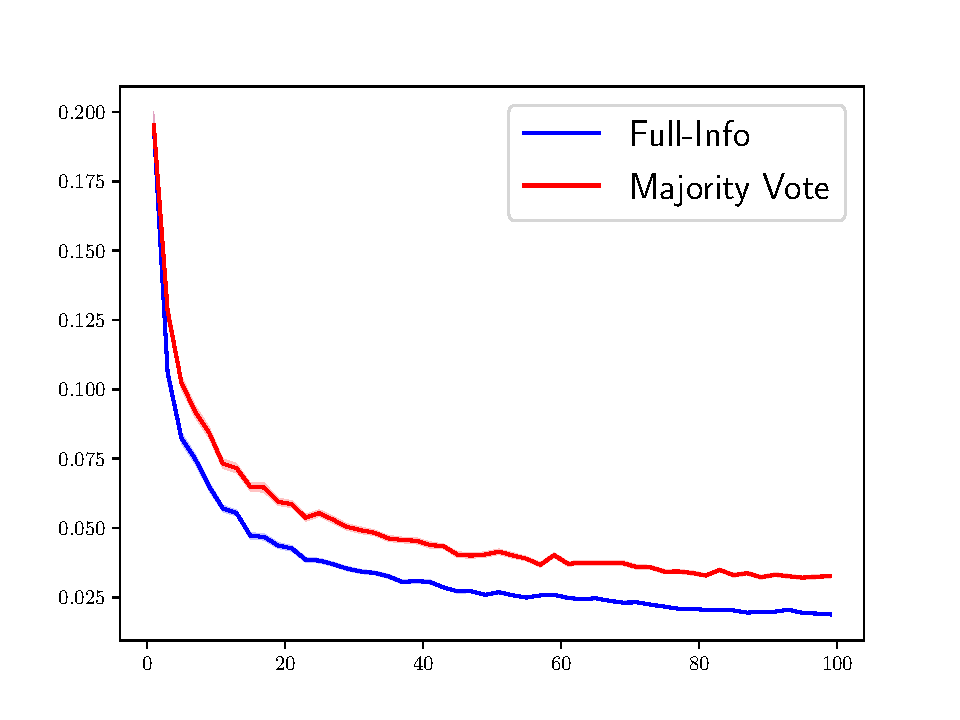
\includegraphics[width=0.3\textwidth]{figure/synthetic-class-05.pdf} &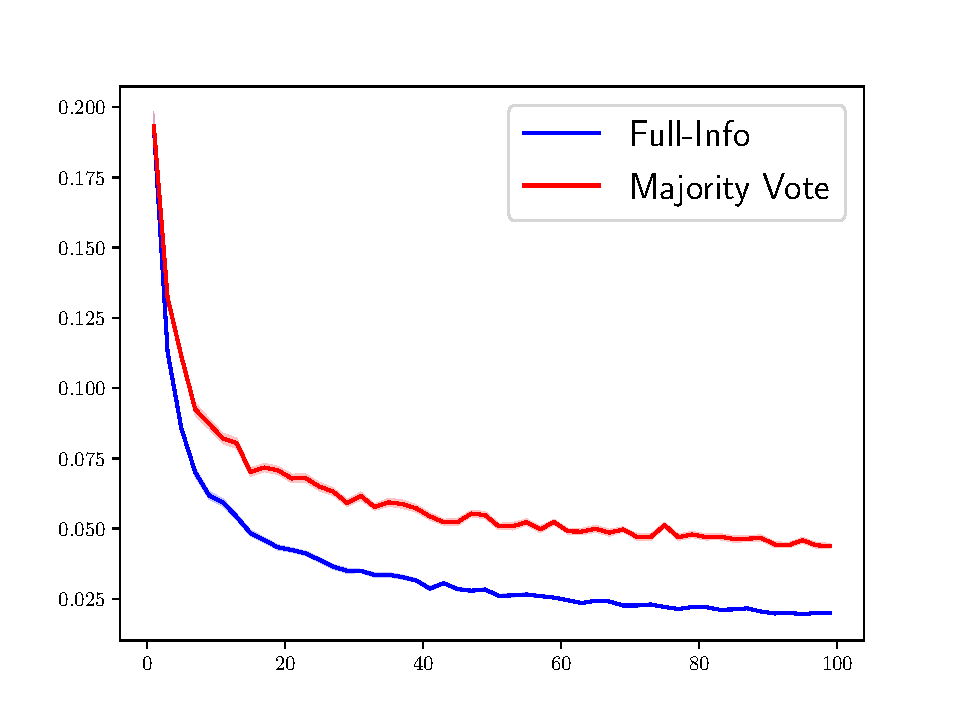
\includegraphics[width=0.3\textwidth]{figure/synthetic-class-10.pdf} &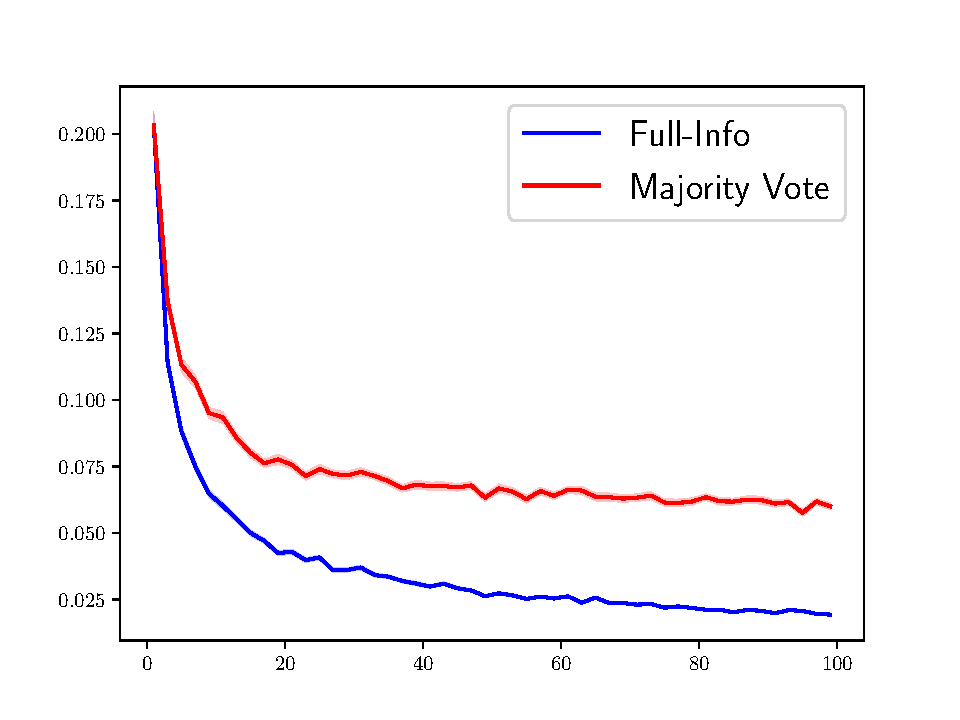
\includegraphics[width=0.3\textwidth]{figure/synthetic-class-15.pdf} \\
%% %		(a) & (b) & (c) \\
%% %		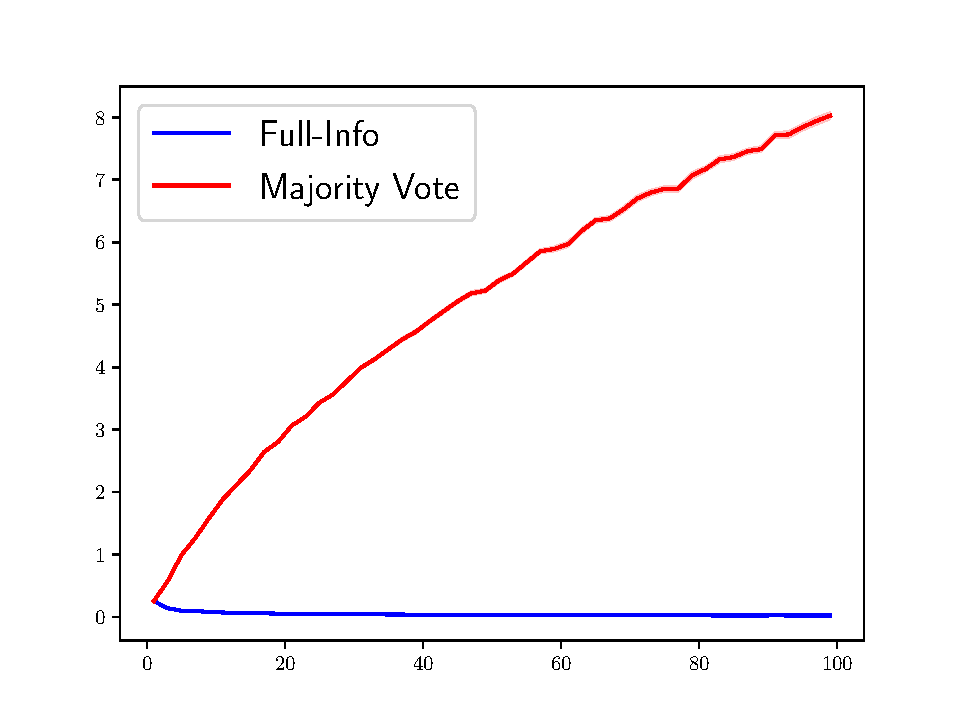
\includegraphics[width=0.3\textwidth]{figure/synthetic-calib-05.pdf} & 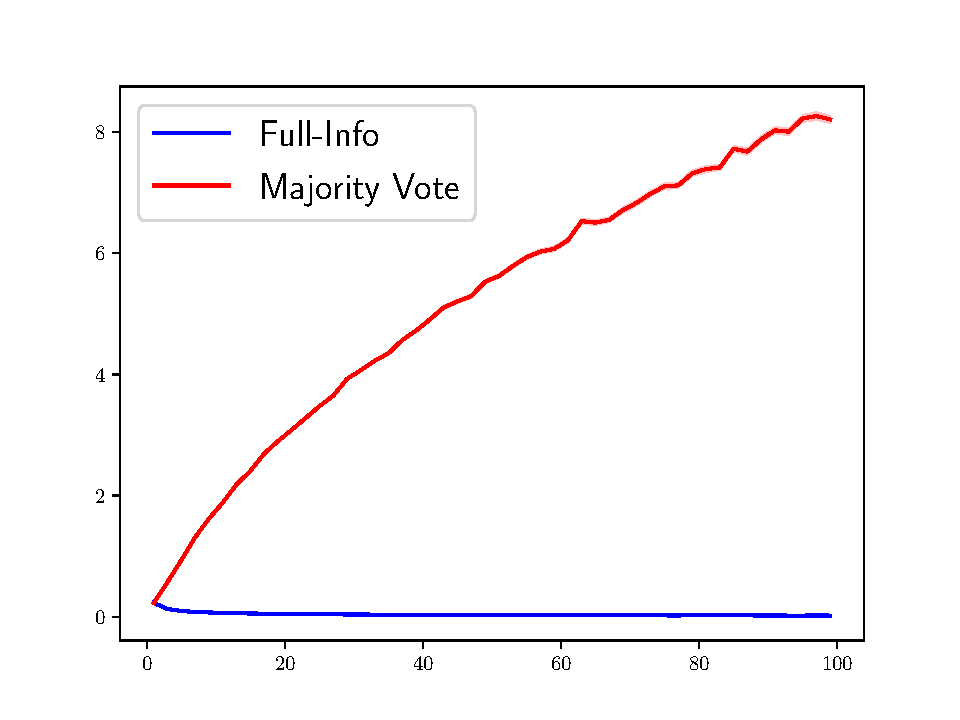
\includegraphics[width=0.3\textwidth]{figure/synthetic-calib-10.pdf} & 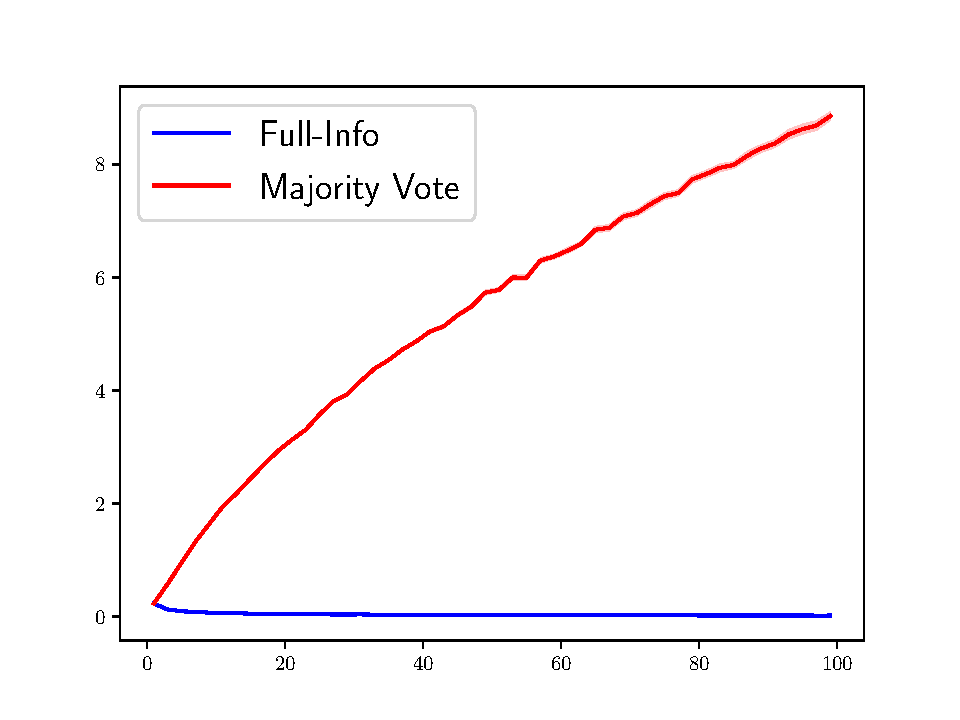
\includegraphics[width=0.3\textwidth]{figure/synthetic-calib-15.pdf}\\
%% %		(a) & (b) &  (c)
%% %	\end{tabular}
%% %	\caption{Classification error and calibration error for synthetic data for $n=1,000$ and $d=10$. For (a) $\beta = 0.5$; For (b) $\beta = 1$; For (c) $\beta = 1.5$. The errors are averaged over 100 trials with 95\% confidence bands.} \label{fig:synthetic}
%% %\end{figure}\ha{can we have only one legend in the plot?}



\subsection{BlueBirds}
\label{sec:BB}

We begin with the
\href{https://github.com/eaplatanios/noisy-labels}{BlueBirds}
dataset~\cite{WelinderBrPeBe10}, a small dataset of 108 images with ResNet features.  The task is to classify each image as one of
\textit{Indigo Bunting} or \textit{Blue Grosbeak} (two similar-looking blue
bird species). For each image, we have $39$ labels, obtained through Amazon
Mechanical Turk workers.  We use an ImageNet pretrained
ResNet50 model to generate image
features, applying PCA to reduce the dimensionality from
$d_{\textup{init}} = 2048$ to $d=25$.

We repeat the following experiment $T = 100$ times.
%
For each number $m = 1, \ldots, 35$ of labelers, we fit
the multi-label logistic model~\eqref{eq:maximum-likelihood}
and the majority vote estimator~\eqref{eq:logistic-majority},
finding calibration and classification errors using 10-fold cross validation.
%
We measure calibration error on an example $x$
by $|\logit(\wt{p}(x)) -
\logit(\what{p}(x))|$, where $\wt{p}(x)$ is the predicted probability,
$\what{p}(x)$ the empirical labeler probability,
and $\logit(p) = \log\frac{p}{1 - p}$; we measure classification
error on example $x$ with
labels $(y_1, \ldots, y_m)$ by $\frac{1}{m} \sum_{j = 1}^m \ind\{y_j \neq
\sgn(\wt{p}(x) - \half)\}$, giving an inherent noise floor because
of labeler uncertainty. We
report the results in Figure~\ref{fig:bluebird}.
These plots corroborate
our theoretical predictions: as the number of labelers $m$ increases, both
the majority vote method and the full label method exhibit improved
classification error, but considering all labels gives a (significant)
improvement in accuracy and in calibration error.

%we train the last layer of a pre-trained model \ha{which dataset for pretraining?} using the two algorithms of interest.
%
%
% \ha{why} and the images are noisy \ha{what does that mean?}.
%For each image
%The dataset was constructed by labels of 39 Amazon MTurk workers, with each of them labeling every image \textit{Indigo Bunting} or \textit{Blue Grosbeak}. For each image $i$, we generate their features $x_i \in \R^d$ by first taking the last layer outputs of a pretrained neural network $\tilde{x}_i \in \R^D$ and using PCA to reduce $\begin{bmatrix} \tilde{x}_1 & \cdots & \tilde{x}_n \end{bmatrix}^\top \in \R^{n \times D}$ to $\begin{bmatrix} x_1 & \cdots & x_n \end{bmatrix}^\top \in \R^{n \times d}$. The plots are shown in Fig.~\ref{fig:bluebird}.



\begin{figure}[ht]
  %% \vspace{-.6cm}
  \begin{center}
    \begin{tabular}{cc}
      \begin{overpic}[width=.48\columnwidth]{%,grid]{%
	  figure/resnet-class-bluebirds.pdf}
	\put(30,-1){{\small Number of labelers $m$}}
	\put(-3,20){
	  \rotatebox{90}{{\small Classification error}}}
      \end{overpic} &
      \hspace{-.3cm}
      \begin{overpic}[width=.48\columnwidth]{%,grid]{%
	  figure/resnet-calib-bluebirds.pdf}
	\put(30,-1){{\small Number of labelers $m$}}
	\put(-3,20){
	  \rotatebox{90}{{\small Calibration error}}}
      \end{overpic} \\
      (a) & (b)
    \end{tabular}
    \caption{\label{fig:bluebird} Experiments on BlueBirds dataset. (a)
      Classification error.  (b) Calibration error $|\logit(\wt{p}) -
      \logit(p)|$ with ResNet features reduced via PCA to dimension
      $d=25$. Error bars show 2 standard error confidence
      bands over $T = 100$ trials.}
  \end{center}
\end{figure}



\subsection{Crowdsourcing methods on semisynthetic CIFAR-10 labels}
\label{sec:semi-synthetic}


\newcommand{\softmax}{\textup{softmax}}

We adapt the original
CIFAR-10 dataset~\cite{KrizhevskyHi09}, which consists of 6000 $32 \times
32$ images from each of $k = 10$ classes (60,000 total images).
%
To mimic collecting messy data, rather than the single-label
in the base CIFAR-10 data, we construct pseudo-labelers
using a pretrained eighteen layer residual network
$f: \mc{X} \to \R^k$ (ResNet18~\cite{HeZhReSu16}) whose accuracy we can
adjust.
%
For $s \in \R^k$, define $\softmax(s) = [e^{s_y} /
  \sum_{l = 1}^k e^{s_l}]_{y = 1}^k$.
%
Then for an input $x \in \mc{X}$, the model outputs a score $f(x)
= {\Theta\opt}^\top \phi(x) \in \R^k$, where
$\Theta\opt = [\theta_1\opt ~ \cdots ~ \theta_k\opt] \in \R^{d \times k}$
is a matrix of per-class weights and
$\phi : \mc{X} \to \R^d$ represents the second-to-last layer
outputs of the neural network.
%
%% \in
%% \R^k$, where $\softmax(f(x))$ indicates the probabilities $\P(Y = y \mid X =
%% x)$.  The model $f$ has the form
%% \begin{equation*}
%%   f(x) = {\Theta\opt}^\top \phi(x), \qquad \text{s.t. }\Theta\opt = [\theta\opt_1 ~ \cdots ~ \theta\opt_k] \in \R^{d \times
%%   	k},
%% \end{equation*}
%% where $\Theta\opt$ is a matrix of per-class weights, and $\phi : \mc{X} \to \R^d$
%% represents the second-to-last layer outputs of the neural network. 
%
As we fit linear models, we take the outputs $\phi(x_i)$ as data, so
$X_i = \phi(x_i)$ are the covariates for the $i$th image $x_i$,
and $\Theta\opt$
is the ground-truth parameter.  We construct labels $Y_{ij}
\in \{1, \ldots, k\}$, $j = 1, \ldots, m$
by choosing the constant $\alpha > 0$
to model labeler expertise, drawing
\begin{equation*}
  \P(Y_{ij} = y \mid X_i = x)
  = \softmax(\alpha f(x))_y
  %% = \softmax(\alpha {\Theta\opt}^\top \phi(x))_y
  = \frac{\exp(\alpha \<\theta\opt_y, \phi(x)\>)}{
    \sum_{l = 1}^k \exp(\alpha \<\theta\opt_l, \phi(x)\>)}.
\end{equation*}
We vary $\alpha$ in experiments to adjust that the median value
of $p_i \defeq \max_{y \in [m]} \softmax(\alpha f(x_i))_y$, where
$p_i \in (1/k, 1)$. In the ``expert labelers'' case, we take
$\alpha \to \infty$ so that $\mbox{median}(\{p_i\}) \to 1$,
while the ``crowd labelers'' case corresponds to
$\alpha \downarrow 0$ and $\mbox{median}(\{p_i\}) \to 1/k$.

We fit $\mve$ and
$\what{\theta}^{\textup{mle}}_{n,m}$ using the multiclass logistic loss.
%
To test our predictions, we also investigate the standard
Dawid-Skene (DS)~\cite{DawidSk79} and GLAD~\cite{WhitehillWuBeMoRu09}
crowdsourcing methods.
%
The DS method models the probability that labeler $j$ assigns label $y'$
given correct label $y$ through a matrix $\alpha_j \in \R^{k \times k}$ with
$p_j(y' \mid y) = \frac{1}{1 + e^{-\alpha_j(y', y)}}$, while GLAD estimates
the probability that labeler $j$ correctly identifies the label of an
example $i$ via $p_{ij} = \frac{1}{1 + e^{-\beta_i \alpha_j}}$, where
$\alpha_j \in [-\infty,\infty]$ indicates labeler $j$'s ability and
$\beta_i \in [0, \infty]$ ambiguity in example $i$.
%
Each method uses EM to approximately maximize the likelihood $\prod_{i =
  1}^n \prod_{j = 1}^m \Prb(Y_{ij} \mid \alpha_j, \beta_i)$ (letting
$\beta_i = 1$ for DS) of the observed labels $Y_{ij}$,
initializing $\alpha$ to maximize the likelihood $\prod_{i = 1}^n \prod_{j
  = 1}^m \Prb(Y_{ij} \mid \majY_i, \alpha_j, \beta_i)$ assuming the majority
votes $\majY_i$ are correct and $\beta_i = 1$.
%
Given estimates $\what{\alpha}$ and $\what{\beta}$, one may impute soft
labels $\what{p}_i \in \R_k^+$ for each example $i$, where $\what{p}_{iy}$
indicates the method's estimated probability that example $i$ is of class
$y$, and hard labels $\what{Y}_i = \argmax_y \what{p}_{iy}$.
%
The labels yield  estimators from, respectively, hard and soft labels via
\begin{equation*}
  \what{\theta}_{\textup{h}}
  = \argmin_{\theta_1, \ldots, \theta_k}
  \sum_{i = 1}^n \log\bigg(\sum_{l = 1}^k
  e^{\<X_i, \theta_l - \theta_{\what{Y}_i}\>}\bigg)
  % \exp(\<X_i, \theta_l - \theta_{\what{Y}_i})\right)
  ~~ \mbox{and} ~~
  \what{\theta}_{\textup{s}}
  = \argmin_{\theta_1, \ldots, \theta_k}
  \sum_{i = 1}^n
  \sum_{y = 1}^k
  \what{p}_{iy} \log\bigg(\sum_{l = 1}^k
  e^{\<X_i, \theta_l - \theta_y\>} \bigg).
  % \exp(\<X_i, \theta_l - \theta_y\>\right),
\end{equation*}
We let $\dse$
and $\glade$ denote the corresponding estimators using hard labels,
and $\dspe$ and $\gladpe$ those trained with the estimated
probabilities $\what{p}_i$.
%
Our experiments use
Crowd-Kit~\citep{UstalovPaTs24}.

\begin{figure}[ht]
  %% \vspace{-.6cm}
  \begin{center}
    \begin{tabular}{cc}
      \hspace{-2cm}
      \begin{overpic}[width=.65\columnwidth]{%,grid]{%
	  figure/hard-test-error.pdf}
      \end{overpic} &
      \hspace{-2.5cm}
      \begin{overpic}[width=.65\columnwidth]{%,grid]{%
	 figure/soft-test-error.pdf}
      \end{overpic} \\
      \hspace{-2cm} (a) &
      \hspace{-2.5cm} (b) \\
      \hspace{-2cm}
      \begin{overpic}[width=.5\columnwidth]{%,grid]{%
	  figure/105.pdf}
      \end{overpic} &
      \hspace{-2.5cm}
      \begin{overpic}[width=.5\columnwidth]{%,grid]{%
	  figure/42.pdf}
      \end{overpic} \\
      \hspace{-2cm} (c) & \hspace{-2.5cm} (d)
    \end{tabular}
    \caption{\label{fig:semisynthetic} Experiments on semisynthetic
      CIFAR-10 dataset. Median labeler accuracy represents the
      median of $p_i = \max_y \softmax(\alpha f(x_i))_y$
      on the training data. Results are
      averaged over $20$ trials, and vertical axes
      give mis-classification rate from (synthetic) ground-truth labels
      on held-out test set. Legend keys correspond to
      maximum likelihood $\what{\theta}^{\textup{mle}}_{n,m}$ (MLE),
      majority vote $\mve$ (MV), hard-labeled Dawid-Skene (DS) and
      GLAD crowdsourced estimators $\dse$ and $\glade$,
      and soft-labaled Dawid-Skene (DS prob) and GLAD (GLAD prob)
      estimators $\dspe$ and $\gladpe$.
      (a) Comparison of methods using hard labels.
      (b) Comparison with crowdsourced estimated soft-labels.
      (c) Number of labelers $m$ versus test error for
      median accuracy $p = .105$ (noisy labelers). (d)
      Number of labelers $m$ versus test error for
      median accuracy $p = .4$. Both (c) and (d) report
      95\% error bars over the trials.}
  \end{center}
\end{figure}

We report the results in Fig.~\ref{fig:semisynthetic}. As we see,
when the model is well-specified,
the MLE $\what{\theta}^{\textup{mle}}_{n,m}$ %%with soft labels 
outperforms aggregation methods and black-box crowdsourcing models that
generate soft labels. Crowdsourced $\dse$ and
$\glade$ yield smaller test error than $\mve$, and using the soft labels,
$\dspe$ and $\gladpe$ further reduces the error, suggesting benefits
to using soft labels from crowdsourcing for training even if the
underlying model is unknown.

\section{Discussion and extensions}

\paragraph{Semi-parametric approaches.}
\label{sec:semi-param}
\label{sec:master-results-sem}

Our analysis separates likelihood-based approaches using all the labels, as
in~\eqref{eq:maximum-likelihood}, and majority vote estimators, which are
robust but have slower convergence, as in
Proposition~\ref{prop:lowd-misspcfd-majority-vote-m}.
%
While we mainly focus on efficiency bounds for 
procedures we view as closer to practice,
%---fitting a model based on available data---
in this section, we
present a few extensions to semiparametric approaches, more
as an amuse-bouche to motivate further efficiency investigations
rather than as a final word.
%% We thus develop a few convergence results into which we can substitute
%% semiparametric estimators.
%
In distinction from standard results in semiparametric theory
(e.g.~\cite[Ch.~25]{VanDerVaart98} or~\cite{BickelKlRiWe98}), the results
require little more than consistent estimation of the links $\sigma_j\opt$
to recover (rate optimal) $1/m$ scaling in the asymptotic covariance.

Let $\vec{\sigma} = (\sigma_1, \ldots, \sigma_m)$
be potentially distinct labeler link functions
(with $\sigma_j\opt$ denoting the true links).
Then for
$(x, y) \in \R^d \times \{\pm 1\}^m$ define the link-based loss
\begin{equation*}
  \loss_{\vec{\sigma}, \theta}(y \mid x)
  \defeq \frac{1}{m} \sum_{j = 1}^m \loss_{\sigma_j,\theta}(y_j \mid x).
\end{equation*}
%
To eliminate ambiguity in $\vec{\sigma}$,
we normalize $\ltwo{\theta\opt} = 1$,
and then define the population loss
\begin{equation*}
	L(\theta, \vec{\sigma})
	\defeq \frac{1}{m} \sum_{j = 1}^m
	\E[\loss_{\sigma_j, \theta}(Y_j \mid X)].
\end{equation*}
For the sequence $\{\vec{\sigma}_n\} \subset \fsymlinksp$
of (estimated) links and data $(X_i,
Y_i)$, $Y_i = (Y_{i1}, \ldots, Y_{im})$, we define the semi-parametric
estimator
\begin{align*}
	\spe \defeq \argmin_{\theta \in \R^d}
	\frac{1}{n} \sum_{i = 1}^n
	\loss_{\vec{\sigma}_n, \theta}(Y_i \mid X_i).
\end{align*}

Both consistency and
asymptotic normality hold under appropriate convergence of
the link functions (see Appendix~\ref{sec:semi-supp} for details).
Define the distance $d_{\flink}$ on $\R^d
\times \flink$ by
\begin{align}
  d_{\flink}\left((\theta_1, \vec{\sigma}_1), (\theta_2, \vec{\sigma}_2)
  \right)
  \defeq
  \ltwo{\theta_1 - \theta_2}
  + \LtwoPbold{\vec{\sigma}_1(-Y\<X, u\opt\>)
    - \vec{\sigma}_2(-Y\<X, u\opt\>)}.
  \label{eqn:link-distance}
\end{align}
%We make the following assumption.
%\begin{assumption}
%	\label{assumption:sp-general}
%	The links $\vec{\sigma}\opt \in \fsymlinksp$ are normalized so
%	that $\P(Y_j = y \mid X = x) = \sigma\opt_j(y \<x, u\opt\>)$, and
%	the sequence $\{\vec{\sigma}_n\} \subset \fsymlinksp$ is consistent:
%	\begin{equation*}
%		\LtwoPbold{\vec{\sigma}_n(-Y\<X, u\opt\>)
%			- \vec{\sigma}\opt(-Y\<X, u\opt\>)}
%		\cp 0.
%	\end{equation*}
%	Additionally, the mapping $(\theta, \vec{\sigma}) \mapsto
%	\nabla_\theta^2 \poploss(\theta,
%	\vec{\sigma})$ is continuous for $d_{\fsymlinksp}$ at $(u\opt,
%	\vec{\sigma}\opt)$.
%\end{assumption}
%The continuity of $\nabla_\theta^2 \poploss(\theta, \vec{\sigma})$ 
%%$\nabla_\theta^2 \poploss(\theta, \vec{\sigma})$ at
%%$(u\opt, \vec{\sigma}\opt)$ 
%allows us to develop local asymptotic normality.
%To see we may expect the assumption to hold, we give reasonably simple
%conditions sufficient for it in Lemma~\ref{lem:d-continuity-guarantees}, Appendix~\ref{sec:semi-supp}.
Then
the next master result for semi-parametric
approaches characterizes the asymptotic behavior of the
semi-parametric estimator $\spe$ using the variance function
\begin{align*}
  C_{m, \vec{\sigma}\opt} := \frac{1}{m} \cdot
  \frac{\frac{1}{m} \sum_{j = 1}^m \E[\sigma_j\opt(Z) (1 - \sigma_j\opt(Z))]}{
    (\frac{1}{m} \sum_{j = 1}^m
    \E[{\sigma_j\opt}'(Z)])^2}.
\end{align*} 
\begin{theorem}
  \label{theorem:semiparametric-master-informal}
  Let Assumption~\ref{assumption:x-decomposition} hold and assume $|Z| > 0$
  has nonzero and continuous density $p(z)$ on $(0, \infty)$.  Suppose the
  sequence $\{\vec{\sigma}_n\}$ is consistent, i.e.,
  \begin{equation*}
    \LtwoPbold{\vec{\sigma}_n(-Y\<X, u\opt\>)
      - \vec{\sigma}\opt(-Y\<X, u\opt\>)}
    \cp 0,
  \end{equation*}
  the mapping $(\theta, \vec{\sigma}) \mapsto
  \nabla_\theta^2 \poploss(\theta,
  \vec{\sigma})$ is continuous for $d_{\flink}$ at $(u\opt,
  \vec{\sigma}\opt)$, and $\Ep [\ltwo{X}^4] < \infty$.  Then $\sqrt{n}(\spe - u\opt)$ is
  asymptotically normal, and the estimator $\what{u}\sem_{n,m} =
  \spe / \ltwos{\spe}$ satisfies
  \begin{equation*}
    \sqrt{n} \prn{\what{u}\sem_{n,m} - u\opt}
    \cd \normal\prn{0, 	C_{m, \vec{\sigma}\opt}
      \prn{\proj_{u\opt}^\perp \Sigma \proj_{u\opt}^\perp}^\dagger}.
  \end{equation*}
\end{theorem}
\noindent
Notably, Theorem~\ref{theorem:semiparametric-master-informal} exhibits optimal
$1/m$ covariance scaling whenever $\E[{\sigma\opt_j}'(Z)] \gtrsim 1$.

We give two example applications of the general
theory in Appendix~\ref{sec:semi-supp}: the first analyzing a full pipeline
for a single index model setting, which robustly estimates direction $u\opt$,
the link $\sigma\opt$, and then re-estimates $\theta\opt$; the second
assuming a stylized black-box crowdsourcing mechanism that provides
estimates of labeler reliability, highlighting how even in some
crowdsourcing scenarios, there could be substantial advantages to using full
label information.

\paragraph{Future work.}

In spite of the technical detail we require to prove our results,
we view this work as almost preliminary and hope that it inspires further
work on the full pipeline of statistical machine learning,
from dataset creation to model release.
%
Many questions remain.

On the theoretical side, we focus on a stylized model of
label aggregation, with majority vote---with the exception of the
crowdsourcing model above--functioning as the
stand-in for more sophisticated aggregation strategies. It seems challenging
to show that \emph{no} aggregation strategy can work as well as multi-label
strategies; it would be interesting to delineate the benefits
and drawbacks of more sophisticated denoising.
% We
% focus throughout on low-dimensional asymptotics, using asymptotic normality
% to compare estimators. 
Additionally, the insights make low-dimensional asymptotic predictions;
investigating high-dimensional scaling might yield new perspectives
as, for, classification datasets often become
separable~\cite{CandesSu19pnas}.
%%, which is consistent with modern
%%applied machine learning~\cite{ZhangBeHaReVi21}.
%but makes the asymptotics we
% derive impossible. One option
% is to investigate the asymptotics of maximum-margin estimators,
% which coincide with the limits of ridge-regularized logistic
% regression~\cite{RossetZhHa04, SoudryHoNaGuSr18}.

On the methodological and applied side, given the extent to which the
test/challenge dataset methodology drives progress in machine
learning~\cite{Donoho17}, it seems that developing newer datasets to
incorporate labeler uncertainty could yield substantial benefits.  A
particular refrain is that modern deep learning methods are overconfident in
their predictions~\cite{GoodfellowShSz15}; perhaps by
calibrating them to \emph{labeler} uncertainty we could
improve their robustness and performance.
%
Large-scale
models now frequently use only distantly supervised
labels~\cite{RadfordKiHaRaGoAgSaAsMiClKrSu21}, making
the study of appropriate data cleaning and collection more timely.
We look forward to deeper
investigations of the foundations of the full
practice of statistical machine learning.


%\subsection*{Support}
%
%This research was partially supported by the Office of Naval Research under
%awards N00014-19-2288 and N00014-22-1-2669, the Stanford DAWN Consortium,
%and the National Science Foundation grants IIS-2006777 and HDR-1934578.

\spacingset{1.87}

\documentclass[12pt]{article}
\usepackage{amsmath}
\usepackage{bibentry}
\usepackage{graphicx}
\usepackage{booktabs}
\usepackage{multirow}
\usepackage{url} % not crucial - just used below for the URL 

%\usepackage[final]{changes}
\usepackage[draft]{changes} 
\newcommand{\stkout}[1]{\ifmmode\text{\sout{\ensuremath{#1}}}\else\sout{#1}\fi} 
\setdeletedmarkup{\stkout{#1}}

%\pdfminorversion=4
% NOTE: To produce blinded version, replace "0" with "1" below.
\newcommand{\blind}{1}

% DON'T change margins - should be 1 inch all around.
\addtolength{\oddsidemargin}{-.5in}%
\addtolength{\evensidemargin}{-1in}%
\addtolength{\textwidth}{1in}%
\addtolength{\textheight}{1.7in}%
\addtolength{\topmargin}{-1in}%

\makeatletter
\def\input@path{}
\makeatother

\input{command.tex}

% \usepackage{enumerate}
\usepackage{enumitem}

\newtheorem{claim}{Claim}[section]
\newtheorem{lemma}[claim]{Lemma}
\newtheorem{assumption}{Assumption}
\newtheorem{definition}{Definition}
\newtheorem{theorem}{Theorem}
\newtheorem{example}{Example}
\newtheorem{proposition}{Proposition}
\newtheorem{remark}{Remark}
\newtheorem{corollary}{Corollary}
\renewcommand{\theassumption}{A\arabic{assumption}}
\renewcommand{\bindist}{\mathsf{Bin}}

\usepackage{xr}
\externaldocument{JASA-supp}

\begin{document}

%\bibliographystyle{natbib}

\def\spacingset#1{\renewcommand{\baselinestretch}%
{#1}\small\normalsize} \spacingset{1}

%%%%%%%%%%%%%%%%%%%%%%%%%%%%%%%%%%%%%%%%%%%%%%%%%%%%%%%%%%%%%%%%%%%%%%%%%%%%%%

\if1\blind
{
  \title{\bf How many labelers do you have? \\
  	A closer look at gold-standard labels}
  \author{Chen Cheng\thanks{Department of Statistics, Stanford University; email: \texttt{chencheng@stanford.edu}.} \and
  	Hilal Asi\thanks{Department of Electrical Engineering, Stanford University; email: \texttt{asi@stanford.edu}.}
  	\and
  	John Duchi\thanks{Departments of Statistics and Electrical Engineering, Stanford University; email: \texttt{jduchi@stanford.edu}.}}
  \maketitle
} \fi

\if0\blind
{
  \bigskip
  \bigskip
  \bigskip
  \begin{center}
    {\LARGE\bf How many labelers do you have? \\
    	A closer look at gold-standard labels}
\end{center}
  \medskip
} \fi

\bigskip

\input{abstract.tex}

\noindent%
{\it Keywords:} Label aggregation, classification and calibration, crowdsourcing
\vfill

\newpage
\spacingset{1.87} % DON'T change the spacing!

\input{intro.tex}
\input{related.tex}
\input{well-specified-theory.tex}
\input{mis-specified-theory.tex}
\input{lower-bound.tex}
%\input{semiparametric-theory.tex}
\input{experiment.tex}
\input{discussion.tex}

%\subsection*{Support}
%
%This research was partially supported by the Office of Naval Research under
%awards N00014-19-2288 and N00014-22-1-2669, the Stanford DAWN Consortium,
%and the National Science Foundation grants IIS-2006777 and HDR-1934578.

\spacingset{1.87}

\input{JASA-main.bbl}

\end{document}


\end{document}


\end{document}


\end{document}
